\documentclass[twoside]{article}


%----------------------------------------------------------------------------------------
%	REQUIRED PACKAGES and commands
%----------------------------------------------------------------------------------------
\usepackage{amsmath,amsfonts,amssymb,amsthm} % For math equations, theorems, symbols, etc
\usepackage{titlesec} % Allows customization of titles
\usepackage{graphicx}        % Required for including pictures
\usepackage{tikz} % Required for drawing custom shapes
\usepackage{enumitem} % Customize lists
\setlist{nolistsep} % Reduce spacing between bullet points and numbered lists
\usepackage[hidelinks]{hyperref} % make a link between the titles in the table of content and the page of it
\usepackage[a4paper, margin=1.2in]{geometry}
\usepackage{blindtext}
\usepackage[skip=9pt plus1pt, indent=0pt]{parskip}
\usepackage{wrapfig}
\usepackage{caption2}
\usepackage{flexisym}
\usepackage{comment}
\usepackage[export]{adjustbox}
\usepackage{tcolorbox} % make the enrichment box 
\usepackage{mathrsfs}
\usepackage{siunitx}	% allow to write the units in math mode
\usepackage{eso-pic} % Required for specifying an image background in the title page
\usepackage{mwe}
\usepackage{booktabs} % Required for nicer horizontal rules in tables
\usepackage{lmodern}
\usepackage[T1]{fontenc}
\usepackage{xcolor}
\hyphenpenalty=10000
\definecolor{Solution}{RGB}{0, 135, 189} 
\allowdisplaybreaks
\usetikzlibrary{positioning,calc}
\usetikzlibrary{patterns}
\newcommand*\circled[1]{\tikz[baseline=(char.base)]{
            \node[shape=circle,draw,inner sep=2pt] (char) {#1};}}
\newcommand{\dquad}{\quad\quad}
\newcommand{\tquad}{\quad\quad\quad}
\newcommand{\fquad}{\quad\quad\quad\quad}



%----------------------------------------------------------------------------------------
%	PDF theme color
%----------------------------------------------------------------------------------------

% \definecolor{theme}{RGB}{13, 71, 161} % Define the color used for highlighting throughout the pdf
% \definecolor{theme}{RGB}{101, 41, 198}
% \definecolor{theme}{RGB}{45, 57, 89}
% \definecolor{theme}{RGB}{0, 0, 150}
\definecolor{theme}{RGB}{51,155,0}


% \definecolor{theme}{RGB}{52, 151, 166}
% \definecolor{theme}{RGB}{243, 102, 25}

%\definecolor{theme}{RGB}{45, 57, 89}
%\definecolor{theme}{RGB}{45, 57, 89}

%----------------------------------------------------------------------------------------
%	MAIN TABLE OF CONTENTS
%----------------------------------------------------------------------------------------

\usepackage{titletoc} % Required for manipulating the table of contents

\contentsmargin{0cm} % Removes the default margin

% section text styling
\titlecontents{section}[1.25cm] % Indentation
{\addvspace{5pt}\large\bfseries} % Spacing and font options for sections
{\color{theme!70}\contentslabel[\Large\thecontentslabel]{1.25cm}\color{theme}} % section number
{}  
{\color{theme!70}\normalsize\bfseries\;\titlerule*[.5pc]{.}\;\thecontentspage} % Page number

% Subsection text styling
\titlecontents{subsection}[1.75cm] % Indentation
{\addvspace{1pt}\small} % Spacing and font options for subsections
{\contentslabel[\thecontentslabel]{1.25cm}} % Subsection number
{}
{\;\titlerule*[.5pc]{.}\;\thecontentspage} % Page number
[] 

% Exclude subsubsection from table of contents
\titlecontents{subsubsection}[2cm] % Indentation
{\addvspace{1pt}\small} % Spacing and font options for subsections
{\contentslabel[\thecontentslabel]{1.25cm}} % Subsection number
{}
{\;\titlerule*[.5pc]{.}\;\thecontentspage} % Page number
[]  




\newtheorem{notation}{Notation}[section]

%%%%%%%%%%%%%%%%%%%%%%%%%%%%%%%%%%%%%%%%%%%%%%%%%%%%%%%%%%%%%%%%%%%%%%%%%%%
%%%%%%%%%%%%%%%%%%%% dedicated to boxed/framed environements %%%%%%%%%%%%%%
%%%%%%%%%%%%%%%%%%%%%%%%%%%%%%%%%%%%%%%%%%%%%%%%%%%%%%%%%%%%%%%%%%%%%%%%%%%
\newtheoremstyle{themenumbox}% % Theorem style name
{0pt}% Space above
{0pt}% Space below
{\normalfont}% % Body font
{}% Indent amount
{\small\bf\color{theme}}% % Theorem head font
{\;}% Punctuation after theorem head
{0.25em}% Space after theorem head
{\small\color{theme}\thmname{#1}\nobreakspace\thmnumber{#2}% Theorem text (e.g. Theorem 2.1)
\thmnote{\nobreakspace\textit\bfseries\color{black}---\nobreakspace#3.}} % Optional theorem note
\renewcommand{\qedsymbol}{$\blacksquare$}% Optional qed square

\newtheoremstyle{blacknumex}% Theorem style name
{5pt}% Space above
{5pt}% Space below
{\normalfont}% Body font
{} % Indent amount
{\small\bf}% Theorem head font
{\;}% Punctuation after theorem head
{0.25em}% Space after theorem head
{\small{\tiny\ensuremath{\blacksquare}}\nobreakspace\thmname{#1}\nobreakspace\thmnumber{#2}% Theorem text (e.g. Theorem 2.1)
\thmnote{\nobreakspace\textit\bfseries---\nobreakspace#3.}}% Optional theorem note

\newtheoremstyle{blacknumbox} % Theorem style name
{0pt}% Space above
{0pt}% Space below
{\normalfont}% Body font
{}% Indent amount
{\small\bf}% Theorem head font
{\;}% Punctuation after theorem head
{0.25em}% Space after theorem head
{\small\thmname{#1}\nobreakspace\thmnumber{#2}% Theorem text (e.g. Theorem 2.1)
\thmnote{\nobreakspace\textit\bfseries---\nobreakspace#3.}}% Optional theorem note

%%%%%%%%%%%%%%%%%%%%%%%%%%%%%%%%%%%%%%%%%%%%%%%%%%%%%%%%%%%%%%%%%%%%%%%%%%%
%%%%%%%%%%%%% dedicated to non-boxed/non-framed environements %%%%%%%%%%%%%
%%%%%%%%%%%%%%%%%%%%%%%%%%%%%%%%%%%%%%%%%%%%%%%%%%%%%%%%%%%%%%%%%%%%%%%%%%%
\newtheoremstyle{themenum}% % Theorem style name
{5pt}% Space above
{5pt}% Space below
{\normalfont}% % Body font
{}% Indent amount
{\small\bf\color{theme}}% % Theorem head font
{\;}% Punctuation after theorem head
{0.25em}% Space after theorem head
{\small\color{theme}\thmname{#1}\nobreakspace\thmnumber{#2}% Theorem text (e.g. Theorem 2.1)
\thmnote{\nobreakspace\textit\bfseries\color{black}---\nobreakspace#3.}} % Optional theorem note
\renewcommand{\qedsymbol}{$\blacksquare$}% Optional qed square

\newtheoremstyle{enbox}% % Theorem style name
{0pt}% Space above
{0pt}% Space below
{}
{}
{}
{}
{0.25em}
{\small
\thmnote{\nobreakspace\textit\bfseries\color{black}---\nobreakspace#3.}} % Optional theorem note
\renewcommand{\qedsymbol}{$\blacksquare$}% Optional qed square


\makeatother

\newcounter{dummy}
\numberwithin{dummy}{section}
\theoremstyle{themenumbox}

\newtheorem{theoremeT}[dummy]{Theorem}

\newtheorem{lemma}[dummy]{Lemma}
\newtheorem{observation}[dummy]{Observation}
\newtheorem{result}[]{Result}
\newtheorem{property}[]{Property}
\newtheorem{proposition}[dummy]{Proposition}
% \newtheorem{definition}[dummy]{Definition}
\newtheorem{claim}[dummy]{Claim}
\newtheorem{fact}[dummy]{Fact}
\newtheorem{assumption}[dummy]{Assumption}

\newtheorem{problem}{Problem}[section]
% \newtheorem{exercise}{Exercise}[section]
\theoremstyle{blacknumex}
\newtheorem{exampleT}{Example}[subsection]
\theoremstyle{blacknumbox}
\newtheorem{vocabulary}{Vocabulary}[section]
\newtheorem{definitionT}{Definition}[section]
\newtheorem{corollaryT}[dummy]{Corollary}




%----------------------------------------------------------------------------------------
%	DEFINITION OF COLORED BOXES
%----------------------------------------------------------------------------------------

\RequirePackage[framemethod=default]{mdframed} % Required for creating the theorem, definition, exercise and corollary boxes

% Theorem box
\newmdenv[
    skipabove=7pt,
    skipbelow=7pt,
    backgroundcolor=black!5,
    linecolor=theme,
    innerleftmargin=5pt,
    innerrightmargin=5pt,
    innertopmargin=5pt,
    leftmargin=0cm,
    rightmargin=0cm,
    innerbottommargin=5pt]{tBox}

% Exercise box	  
\newmdenv[skipabove=7pt,
skipbelow=7pt,
rightline=false,
leftline=true,
topline=false,
bottomline=false,
backgroundcolor=theme!10,
linecolor=theme,
innerleftmargin=5pt,
innerrightmargin=5pt,
innertopmargin=5pt,
innerbottommargin=5pt,
leftmargin=0cm,
rightmargin=0cm,
linewidth=4pt]{eBox}	

% Definition box
\newmdenv[
skipabove=3pt,
skipbelow=3pt,
rightline=false,
leftline=true,
topline=false,
bottomline=false,
linecolor=theme,
innerleftmargin=5pt,
innerrightmargin=5pt,
innertopmargin=0pt,
leftmargin=0cm,
rightmargin=0cm,
linewidth=4pt,
innerbottommargin=0pt]{dBox}	

% Corollary box
\newmdenv[skipabove=7pt,
skipbelow=7pt,
rightline=false,
leftline=true,
topline=false,
bottomline=false,
linecolor=gray,
backgroundcolor=black!5,
innerleftmargin=5pt,
innerrightmargin=5pt,
innertopmargin=5pt,
leftmargin=0cm,
rightmargin=0cm,
linewidth=4pt,
innerbottommargin=5pt]{cBox}

% Creates an environment for each type of theorem and assigns it a theorem text style from the "Theorem Styles" section above and a colored box from above
\newenvironment{theorem}{\begin{tBox}\begin{theoremeT}}{\end{theoremeT}\end{tBox}}
\newenvironment{exercise}{\begin{eBox}\begin{exerciseT}}{\hfill{\color{theme}\tiny\ensuremath{\blacksquare}}\end{exerciseT}\end{eBox}}				  
\newenvironment{definition}{\begin{dBox}\begin{definitionT}}{\end{definitionT}\end{dBox}}	
\newenvironment{example}{\begin{exampleT}}{\hfill{\tiny\ensuremath{\blacksquare}}\end{exampleT}}		
\newenvironment{corollary}{\begin{cBox}\begin{corollaryT}}{\end{corollaryT}\end{cBox}}	
\newenvironment{enrichment*}[1]{\begin{tcolorbox}[colback=theme!5!white,colframe=theme!50!black,title=#1]}{\end{tcolorbox}}



\newenvironment{enrichment}[5]{
    \def\Title{#1}    
    \def\imagepath{#2}
    \def\imagewidth{#3}
    \def\textspace{#4}
    \def\imagespace{#5}
    \begin{tcolorbox}[colback=theme!5!white,colframe=theme!50!black,title=\Title]
        \begin{minipage}[t]{\textspace\textwidth}
        }{
        \end{minipage}
        \hfill
        \begin{minipage}[t]{\imagespace\textwidth}
            \includegraphics[width=\imagewidth cm,valign=t]{\imagepath}
        \end{minipage}
    \end{tcolorbox}
}


%----------------------------------------------------------------------------------------
%	SECTION NUMBERING IN THE MARGIN
%----------------------------------------------------------------------------------------

\makeatletter
\renewcommand{\@seccntformat}[1]{\llap{\textcolor{theme}{\csname the#1\endcsname}\hspace{1em}}}                    
\renewcommand{\section}{\@startsection{section}{1}{\z@}
{-4ex \@plus -1ex \@minus -.4ex}
{1ex \@plus.2ex }
{\normalfont\large\bfseries}}
\renewcommand{\subsection}{\@startsection {subsection}{2}{\z@}
{-3ex \@plus -0.1ex \@minus -.4ex}
{0.5ex \@plus.2ex }
{\normalfont\bfseries}}
\renewcommand{\subsubsection}{\@startsection {subsubsection}{3}{\z@}
{-2ex \@plus -0.1ex \@minus -.2ex}
{.2ex \@plus.2ex }
{\normalfont\small\bfseries}}                        
\renewcommand\paragraph{\@startsection{paragraph}{4}{\z@}
{-2ex \@plus-.2ex \@minus .2ex}
{.1ex}
{\normalfont\small\bfseries}}





\usepackage{fancyhdr}
\usepackage{fontspec}
\usepackage{physics}
\newcommand{\hquad}{\,\,}
\newcommand{\Blankpage}{\newpage \ \newpage}
\newcommand{\hmasafa}{\hspace*{.25cm}}
\newcommand{\vmasafa}{\vspace*{.25cm}}
\tikzset{
  oblique lines/.style={
    pattern = north east lines,
    pattern color = red,
  }
}
\usepackage{multicol}
% \newcommand{\DRL}[4][RL][0][t][\alpha]{\prescript{#1}{#2}{D_{#3}^{#4}}}
\usepackage{ragged2e}
\usepackage{mathtools,leftindex,tensor,mhchem}

%\definecolor{cover}{RGB}{230, 194, 24}

%blue
%\definecolor{cover}{RGB}{51,215,213}

%green
%\definecolor{cover}{RGB}{51,215,153}

%dark green
%\definecolor{cover}{RGB}{51,215,103}

\definecolor{cover}{RGB}{51,215,0}

\definecolor{Golden}{RGB}{202, 184, 41}
\definecolor{DarkGreen}{RGB}{125, 169, 98}
\definecolor{orangered}{RGB}{233, 118, 86}
\definecolor{skyblue}{RGB}{113, 188, 220}
\newfontfamily\Acmefont{Acme-Regular}[
        Path = fonts/Acme/,
        Extension =.ttf
]
\newfontfamily\fancyfont{GreatVibes-Regular}[
        Path = fonts/Great_Vibes/,
        Extension =.ttf
]
\newfontfamily\handfont{PlaypenSans-ExtraBold}[
        Path = fonts/Playpen_Sans/,
        Extension =.ttf
]
\newfontfamily\Garamondfont{EBGaramond-Medium}[
        Path = fonts/Garamond/,
        Extension =.ttf
] 
\newfontfamily\HPfont{HP}[
        Path = fonts/harryp/,
        Extension =.ttf
] 
\numberwithin{equation}{section}

% \pagestyle{fancy}
% \fancyhf{}
% \fancyhead[LO,RE]{\thepage}
% \fancyhead[RO]{\leftmark}
% \fancyhead[LE]{\rightmark}
% \fancyfoot{\hrule}
% \renewcommand{\sectionmark}[1]{\markboth{#1}{}}
% \renewcommand{\subsectionmark}[1]{\markright{#1}}
\usepackage{changepage}

\begin{document}



% %----------------------------------------------------------------------------------------
%	TITLE PAGE
%----------------------------------------------------------------------------------------
\begingroup
\AddToShipoutPicture*{\put(0,0){
\includegraphics[width=\paperwidth,height=\paperheight]{back.jpg}}}
\thispagestyle{empty}
\color{Golden}
\vspace*{15cm}\scalebox{90}{
    \hspace*{-.23cm}
\begin{tikzpicture}[overlay,every node/.style={rotate=6}]
    \draw (0,0) node{$\int$};
\end{tikzpicture}
}
\endgroup

\begingroup
\color{white}

% \begin{tikzpicture}[overlay,every node/.style={scale=.5}]
%     \node at (1,1) {
\includegraphics[scale=.1]{univ.png}};
%     \draw (0,0) node{Alexandria University};
%     \draw (0,0) node{Faculty of Sciences};
%     \draw (0,0) node{Department of Mathematics};
%     \draw (0,0) node{And computer Sciences};
% \end{tikzpicture}

\vspace*{-8cm}
\hspace*{2.5cm}

\begin{tikzpicture}
    \draw (0,.5) node{
        {\fontsize{35pt}{40pt}\selectfont    
    \textbf{Theory \& Applications}
        }
    };
    \draw (0,-1) node{
        {\fontsize{35pt}{40pt}\selectfont    
    \textbf{Of}
        }
    };
    \color{Golden}
    \draw (0,-2.5) node{
        {\fontsize{40pt}{40pt}\selectfont    
    \textbf{Fractional Calculus}
        }
    };
\end{tikzpicture}


\vspace*{8.3cm}
\hspace*{2cm}
\begin{tikzpicture}
    \color{Golden}
    \draw (0,0) node{
        {\fontsize{15pt}{24pt}\selectfont    
    \textbf{By}
        }
    };
    \color{white}
    \draw (0,-1) node{
        {\fontsize{15pt}{0pt}\selectfont    
    \textbf{Ahmed.M. Habib}
        }
    };    
\end{tikzpicture}
% \vspace*{5cm}
\hspace*{2cm}

\begin{tikzpicture}
    \color{Golden}
    \draw (0,0) node{
        {\fontsize{15pt}{0pt}\selectfont    
    \textbf{Supervised By}
        }
    };
    \color{white}
    \draw (0,-1) node{
        {\fontsize{15pt}{24pt}\selectfont    
    \textbf{Dr. Amira Mostafa Abdallah}
        }
    };
\end{tikzpicture}
\endgroup

\newpage
\thispagestyle{empty}

\begingroup
\newgeometry{left=.8in, right=1in, top=.8in}
\begin{center}
    
\includegraphics[scale=.5]{collage logo.png}
    \vspace*{1cm}
    \par
    {\fontsize{20pt}{30pt}\selectfont
        {\fontsize{30pt}{40pt}\selectfont
        \textbf{Theory \& Applications \\ of \\ Fractional Calculus}
        }
        \\
        \vspace*{.75cm}
        By
        \vspace*{.75cm}

        Ahmed Mohamed Abd-Elsalam Habib

        ID : 20211499907

        Department of Mathematics and computer Sciences

        Faculty of Sciences

        Alexandria University

        \vspace*{\fill}
        Under The Supervision Of
        
        Dr. Amira Mostafa Abdallah
    }
\end{center}
\restoregeometry
\endgroup
\newpage
\tableofcontents
\thispagestyle{empty}
\newpage
\setcounter{page}{1}      %The pages it the start

%%%%%%%%%%%%%%%%%%%%%%%%%%%%%%%%%%%%%%%%%%%%%%%%%%%%%%%%%%%%
%%%%%%%%%%%%%%%%%%%%%%%%%%%%%%%%%%%%%%%%%%%%%%%%%%%%%%%%%%%%
%%%%%%%%%%%%%%%%%%%%%%%%%%%%%%%%%%%%%%%%%%%%%%%%%%%%%%%%%%%%
%%%%%%%%%%%%%%%%%%%%%%%%%%%%%%%%%%%%%%%%%%%%%%%%%%%%%%%%%%%%
%%%%%%%%%%%%%%%%%%%%%%%%%%%%%%%%%%%%%%%%%%%%%%%%%%%%%%%%%%%%
%%%%%%%%%%%%%%%%%%%%%%%%%%%%%%%%%%%%%%%%%%%%%%%%%%%%%%%%%%%%
%%%%%%%%%%%%%%%%%%%%%%%%%%%%%%%%%%%%%%%%%%%%%%%%%%%%%%%%%%%%
%----------------------------------------------------------------------------------------
%	TITLE PAGE
%----------------------------------------------------------------------------------------
\begingroup
\AddToShipoutPicture*{\put(0,0){
\includegraphics[width=\paperwidth,height=\paperheight]{front.png}}}
\pagenumbering{roman}
\thispagestyle{empty}
\color{white}

\begin{tikzpicture}[overlay,every node/.style={scale=1}]
    \node at (-1,1) {
\includegraphics[scale=.02]{univ inv.png}};

    \draw (2.2,1.4) node{
        \begin{tabular}{ l }
            Alexandria University
            \\
            Faculty of Sciences
            \\
            Department of Mathematics
            \\
            And Computer Science
           \end{tabular}
           };
        \end{tikzpicture}
\begin{tikzpicture}[overlay,every node/.style={scale=.7}]
        \draw (10,-9) node{
            \begin{tabular}{ c }
                {\fontsize{50pt}{40pt}\selectfont    
                    \textbf{Theory \& Applications}
                }
                \\\\
                {\fontsize{50pt}{40pt}\selectfont    
                    \textbf{Of}
                }
                \\\\
                \color{Golden}
                {\fontsize{55pt}{40pt}\selectfont    
                    \textbf{Fractional Calculus}
                }
            \end{tabular}
            };
        % \draw (10,-9) node{
        % \begin{tabular}{ c }
        %     {\fontsize{80pt}{40pt}\HPfont\selectfont    
        %         \textbf{Theory And Applications}
        %     }
        %     \\\\
        %     {\fontsize{80pt}{40pt}\HPfont\selectfont    
        %         \textbf{Of}
        %     }
        %     \\\\
        %     \color{Golden}
        %     {\fontsize{85pt}{40pt}\HPfont\selectfont    
        %         \textbf{Fractional Calculus}
        %     }
        %     \end{tabular}
        %     };

                   
    \draw (9.5,-24) node{
        \color{red}
        \begin{tabular}{ c c }
            {\fontsize{15pt}{24pt}\selectfont    
                \textbf{By}
            }
            & \hspace*{5cm}
            {\fontsize{15pt}{0pt}\selectfont    
                \textbf{Supervised By}
            }
            \\\\
            \color{white}
            {\fontsize{20pt}{0pt}\selectfont    
                \textbf{Ahmed.M. Habib}
            }
            & \hspace*{5cm}
            \color{white}
            {\fontsize{20pt}{24pt}\selectfont    
                \textbf{Dr. Amira Mostafa Abdallah}
            }
        \end{tabular}
    };

\end{tikzpicture}
\endgroup


\newpage
\thispagestyle{empty}

\begingroup
\newgeometry{left=.8in, right=1in, top=.8in}
\begin{center}
    
\includegraphics[scale=.5]{collage logo.png}
    \vspace*{1cm}
    \par
    {\fontsize{20pt}{30pt}\selectfont
        {\fontsize{30pt}{40pt}\selectfont
        \textbf{Theory \& Applications \\ of \\ Fractional Calculus}
        }
        \\
        \vspace*{.75cm}
        By
        \vspace*{.75cm}

        Ahmed Mohamed Abd-Elsalam Habib

        ID : 20211499907

        Department of Mathematics and computer Sciences

        Faculty of Sciences

        Alexandria University

        \vspace*{\fill}
        Under The Supervision Of
        
        Dr. Amira Mostafa Abdallah
    }
\end{center}
\restoregeometry
\endgroup
\newpage
\thispagestyle{empty}
\vspace*{-2cm}
\tableofcontents
\thispagestyle{empty}
\newpage
\pagenumbering{arabic}
\setcounter{page}{1}        % The pages it the start
% \thispagestyle{empty}
% \section*{\LARGE Acknowledgement}
% \vspace*{1cm}
% I would like to express my sincere gratitude to all those who have contributed to the completion of this project. 

% First and foremost, I extend my heartfelt thanks to my supervisor Dr.Amira Mostafa for their invaluable guidance, support, 
% and encouragement throughout this endeavor. Their expertise and insights have been instrumental in shaping the direction and quality of this work.

% I am grateful to my colleagues and peers for their camaraderie, discussions, and assistance whenever needed. 
% Their diverse perspectives have broadened my understanding and inspired new ideas.

% Last but not least, I extend my appreciation to my family and friends for their unwavering support, 
% patience, and belief in me, which have been the cornerstone of my perseverance.

% This project would not have been possible without the collective effort and support of all those mentioned above. 
% Thank you for being part of this journey and for your invaluable contributions.

% Sincerely,\\
% Ahmed Mohamed Abd-Elsalam Habib

% \newpage 
% \setcounter{page}{1}

\section{Introduction}

\begin{minipage}[t][.18\textheight]{\textwidth}
\begin{wrapfigure}{r}{0.2\textwidth}
    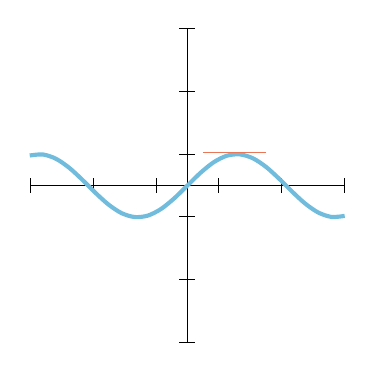
\begin{tikzpicture}[scale=.4]
        % Axes
        \draw[|-|] (-5,0) -- (5,0);
        \draw[|-|] (0,-5) -- (0,5);
        
        \draw[|-|] (-3,0) -- (3,0);
        \draw[|-|] (0,-3) -- (0,3);
    
        \draw[|-|] (-1,0) -- (1,0);
        \draw[|-|] (0,-1) -- (0,1);
        
        % Plot
        \draw[domain=-5:5,line width=1.5pt,smooth,variable=\x,skyblue] plot ({\x},{sin(\x r)});
        \draw[domain=.5:2.5,smooth,variable=\x,orangered] plot ({\x},{1.05});
    \end{tikzpicture}
\end{wrapfigure}
When learning calculus, you are probably accustomed to the idea of higher order derivatives 

\vspace*{1.5cm}
The first derivative $\displaystyle \dv{y}{x}$ indicates the slope of a graph.
\end{minipage}
\par
\begin{minipage}[t][.21\textheight]{\textwidth}
\begin{wrapfigure}{r}{0.2\textwidth}
    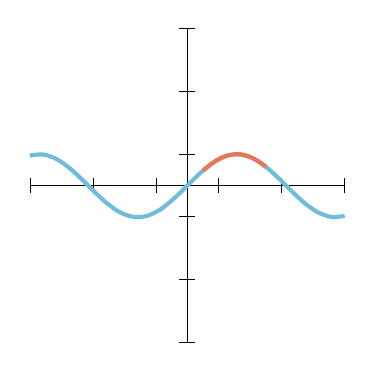
\begin{tikzpicture}[scale=.4]
        % Axes
        \draw[|-|] (-5,0) -- (5,0);
        \draw[|-|] (0,-5) -- (0,5);
        
        \draw[|-|] (-3,0) -- (3,0);
        \draw[|-|] (0,-3) -- (0,3);
    
        \draw[|-|] (-1,0) -- (1,0);
        \draw[|-|] (0,-1) -- (0,1);
        
        % Plot
        \draw[domain=-5:5,line width=1.5pt,smooth,variable=\x,skyblue] plot ({\x},{sin(\x r)});
        \draw[domain=.5:2.5,line width=1.5pt,smooth,variable=\x,orangered] plot ({\x},{sin(\x r)});
    \end{tikzpicture}
\end{wrapfigure}
.

\vspace*{1.8cm}
And the second derivative $\displaystyle \dv[2]{y}{x}$ indicates concavity
\end{minipage}



And so on calculating the $ n^{\text{th}} $ derivative of a function $\displaystyle \dv[n]{f(x)}{x}$ is taking the derivative of it $n$ times 
\[
    \underbrace{\left(\dv{}{x} \dots \dv{}{x}\right)}_{\text{n times}} f(x)
\]
And this made sense but what does it mean to take a fractional derivative
\[
    \dv[\frac{1}{2}]{f(x)}{x} = ???
\]
We're going to be exploring another branch of calculus \textbf{FRACTIONAL CALCULUS}.

The expression $\displaystyle \dv[n]{f(x)}{x}$ can have multiple 
meanings first it can be thought of as a repeated differentiation 
so if we take the $ n^{\text{th}} $ derivative of a function it means taking 
the derivative $n$ times however this only makes sense for 
positive integers if we are to extend this to other numbers 
we must think of this expression as a transformation 
something that takes in a function as an input and gives a 
function as an output 

\begin{center}
    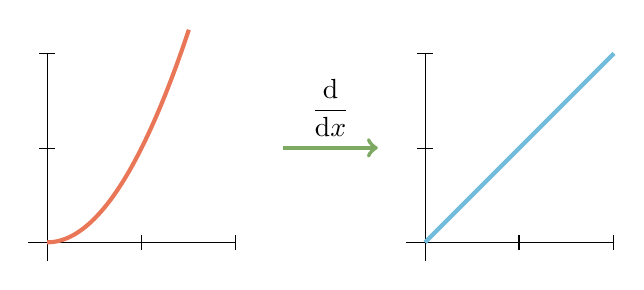
\begin{tikzpicture}[scale=1.2]
        % Axes
        \draw[-|] (-.2,0) -- (2,0);
        \draw[-|] (0,-.2) -- (0,2);
        
        \draw[-|] (0,0) -- (1,0);
        \draw[-|] (0,0) -- (0,1);
        
        % Plot
        \draw[domain=0:1.5,line width=1.5pt,smooth,variable=\x,orangered] plot ({\x},\x*\x);
        
    
        \draw[->, line width=1.5pt,DarkGreen] (2.5,1) -- (3.5,1) node[midway,above,black] {$\displaystyle \dv{}{x}$};
    
        % Axes
        \draw[-|] (3.8,0) -- (6,0);
        \draw[-|] (4,-.2) -- (4,2);
        
        \draw[-|] (4,0) -- (5,0);
        \draw[-|] (4,0) -- (4,1);
        
        % Plot
        \draw[domain=0:2,line width=1.5pt,smooth,variable=\x,skyblue] plot ({\x+4},\x);
    
    \end{tikzpicture}
\end{center}

And not as repeated differentiation 
\\
We will look at $\displaystyle \dv[n]{f(x)}{x}$ as an operator that transforms $f$ into it's $ n^{\text{th}} $ derivative


\section{Fractional Integral}
We will start with the Fractional Integral although integrals are often harder to compute, 
but they often relate more nicely to each other and are less picky about what 
functions you throw into them. 
For example any continuous function can be integrated but NOT every continuous function can 
be differentiated. 
Like the Weierstrass function which is a continuous function that has no derivative anywhere along it due to its fractal jaggedness.
\\
Let's establish a bit of notation $If(x)$ mean the indefinite integral of the function from 0 to $x$
\[
If(x) = \int_{0}^{x} f(t) \hquad dt
\]
As we talked about earlier we can think of this as a transformation something that takes in a function and outputs a function
\begin{center}
    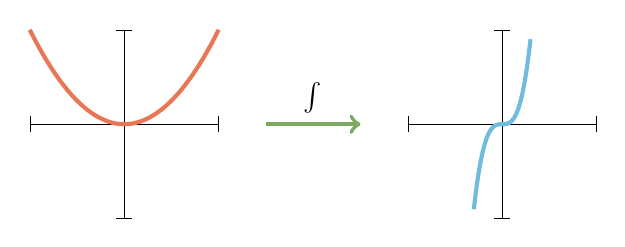
\begin{tikzpicture}[scale=1.2]
        % Axes
        \draw[|-|] (-1,0) -- (1,0);
        \draw[|-|] (0,-1) -- (0,1);
        
        % Plot
        \draw[domain=-1:1,line width=1.5pt,smooth,variable=\x,orangered] plot ({\x},\x*\x);
        
    
        \draw[->, line width=1.5pt,DarkGreen] (1.5,0) -- (2.5,0) node[midway,above,black] {$\int$};
    
        % Axes
        \draw[|-|] (3,0) -- (5,0);
        \draw[|-|] (4,-1) -- (4,1);
        
        \begin{scope}[scale=0.1]
        % Plot
        \draw[domain=-3:3,line width=1.5pt,smooth,variable=\x,skyblue] plot ({\x+40},\x*\x*\x/3);
        \end{scope}

    \end{tikzpicture}
\end{center}
Similar to differentiation we put an exponent like thing to denote the $ n^{\text{th}} $ integral of $f(x)$ 
\\
So for example the third integral would look something like this
\[
I^3 f(x) = \int_{0}^{x}\left[ \int_{0}^{t}\left[ \int_{0}^{s} f(u) \hquad du \right]ds \right]dt
\]
\begin{center}
    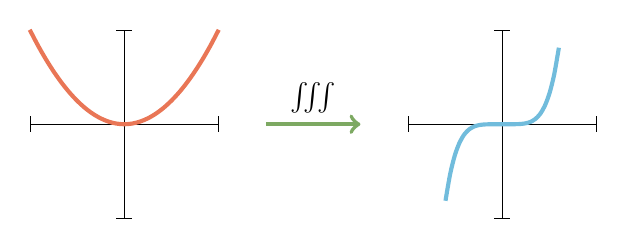
\begin{tikzpicture}[scale=1.2]
        % Axes
        \draw[|-|] (-1,0) -- (1,0);
        \draw[|-|] (0,-1) -- (0,1);
        
        % Plot
        \draw[domain=-1:1,line width=1.5pt,smooth,variable=\x,orangered] plot ({\x},\x*\x);
        
    
        \draw[->, line width=1.5pt,DarkGreen] (1.5,0) -- (2.5,0) node[midway,above,black] {$\iiint$};
    
        % Axes
        \draw[|-|] (3,0) -- (5,0);
        \draw[|-|] (4,-1) -- (4,1);
        
        
        % Plot
        % \draw[domain=-1:1,smooth,variable=\x,blue] plot ({\x+4},\x*\x*\x/3);

        \begin{scope}[scale=0.2]
            % Plot
            \draw[domain=-3:3,line width=1.5pt,smooth,variable=\x,skyblue] plot ({\x+20},\x*\x*\x*\x*\x/60);
        \end{scope}
    
    \end{tikzpicture}
\end{center}
\subsection{Cauchy's Repeated Integration Formula}
As we increase the number the expression gets more and more complicated 
But Cauchy found a way to look at 
repeated integrals like this and put it in the form of a single integral of convolution type
which is Cauchy's Formula for Repeated Integration.

First we take the integral of a function $f(t)$
\begin{figure*}[b]
    \begin{minipage}[h]{\textwidth}
        \begin{enrichment}{Augustin Louis Cauchy}{Chars/Cauchy.jpg}{2.4}{.8}{.17}
            Baron Augustin-Louis Cauchy (1789-1857) was a French mathematician and physicist 
            he's well known the most for his significant contributions in analysis, calculus, and number theory 
            although he didn't make direct contributions to fractional calculus in the way we understand 
            it today, his integral formula provided a crucial tool for mathematicians who later 
            explored this area. 
            Essentially, Cauchy's formula helped establish the foundation for defining fractional 
            differentiation and integration.
        \end{enrichment} 
    \end{minipage}
\end{figure*}
\[
    If(t) = \int_{0}^{t} f(s) \hquad ds
\]
Repeating this process gives 
\[
    I^2 f(t) = \int_{0}^{t} If(s) \hquad ds  = \int_{0}^{t}\int_{0}^{s} f(\theta) \hquad d\theta \hquad ds 
\]
\begin{minipage}[t][.18\textheight]{\textwidth}
    \begin{wrapfigure}{r}{0.2\textwidth}
        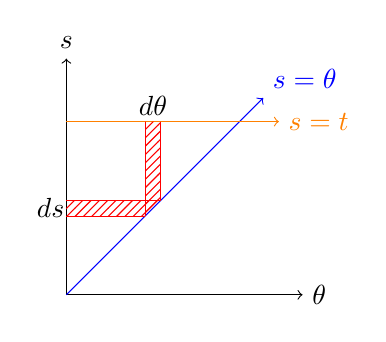
\begin{tikzpicture}
            \draw[->] (0,0,0) -- (3,0,0) node[right]{$\theta$};
            \draw[->] (0,0,0) -- (0,3,0) node[above]{$s$};
            \draw[->, blue] (0,0,0) -- (2.5,2.5,0) node[above right]{$s = \theta$};
            \draw[->, orange] (0,2.2,0) -- (2.7,2.2,0) node[right]{$s = t$};
        
            \draw[-,red] (0,1,0)--(1,1,0);
            \draw[-,red] (0,1.2,0)--(1.2,1.2,0);
        
            \fill [oblique lines] (0,1,0) -- (1,1,0) -- (1.2,1.2,0) -- (0,1.2,0);
            \fill [oblique lines] (1,1,0) -- (1,2.2,0) -- (1.2,2.2,0) -- (1.2,1.2,0);
        
            \draw[-,red] (1,1,0)--(1,2.2,0);
            \draw[-,red] (1.2,1.2,0)--(1.2,2.2,0);
        
            \draw (-.2,1.1,0) node{$ds$};
            \draw (1.1,2.4,0) node{$d\theta$};
        \end{tikzpicture}
    \end{wrapfigure}
We can interchanging the order of integration using Fubini's theorem
\[
    I^2 f(t) = \int_{0}^{t}\int_{\theta}^{t} ds \hquad f(\theta) \hquad d\theta = \int_{0}^{t}(t-\theta)f(\theta) \hquad d\theta
\]
Similarly we can get $I^3f(t)$
\begin{align*}
    I^3 f(t) &= \int_{0}^{t} \int_{0}^{s} (s-\theta)f(\theta) \hquad d\theta \hquad ds
             \\
             &= \int_{0}^{t} \frac{(t-\theta)^2}{2}f(\theta) \hquad d\theta = \int_{0}^{t} \frac{(t-\theta)^2}{2!}f(\theta) \hquad d\theta
\end{align*}
\end{minipage}

\vspace*{.3cm}
And so on we can get 
\begin{equation}
    I^n f(t) = \int_{0}^{t} \frac{(t-\theta)^{n-1}}{(n-1)!}f(\theta) \hquad d\theta \quad , \quad n=1,2,3,\dots
\end{equation}
\subsection{Riemann-Liouville Integral}
Now the real question is how do we define this formula for any positive number ?
\\
The answer lies within the gamma function $\Gamma(n)$.
\begin{figure*}[b]
    \begin{minipage}[h]{\textwidth}
        \begin{enrichment}{Bernhard Riemann}{Chars/Riemann.jpg}{2.4}{.8}{.17}
            Though he is best known for his contributions to geometry and analysis, 
            he also made huge steps in the development of fractional calculus. 
            While not published until after his death, Riemann's work explored a definition for 
            fractional integration laid the groundwork for what is now known as the Riemann-Liouville 
            fractional integral, a cornerstone of the field.
        \end{enrichment} 
    \end{minipage}
\end{figure*}
\begin{figure*}[b]
    \begin{minipage}[h]{\textwidth}
        \begin{enrichment}{Joseph Liouville}{Chars/Joseph Liouville.jpg}{2.4}{.8}{.17}
            Joseph Liouville deserves credit for sparking the entire field of fractional calculus. 
            Even earlier than Riemann, Liouville, in 1832, first proposed the idea of generalizing 
            derivatives and integrals to non-integer orders. 
            While he didn't establish a complete framework, Liouville's pioneering thought and experiment 
            opened the door for mathematicians like Riemann to develop the specific definitions and tools used in fractional calculus today.
        \end{enrichment} 
    \end{minipage}
\end{figure*}


\begin{enrichment*}{Gamma Function}
    The Gamma Function is defined as follows
    \[
    \Gamma(n) = \int_{0}^{\infty} e^{-t} t^{n-1} \hquad dt \quad , \quad \forall n>0
    \]  
    And has the following properties
    \begin{itemize}
        \item $\Gamma(n+1) = n \Gamma(n)$
        \item $\Gamma(n+1) = n!$
        \item $\Gamma(1) = 1 \quad;\quad \Gamma(\frac{1}{2}) = \sqrt{\pi} $
    \end{itemize}
    The goal of the gamma function was to define a smooth 
    curve that would go through factorial points 

    It gives us a way to extend the domain of factorials 
    from positive integers to the positive real numbers 
    and even the complex numbers for $Re(n) \notin \mathbb{Z}^- \cup \{0\} $ 
\end{enrichment*}
Since the main thing restricting the domain of a formula 
for repeated integration (2.1) is the factorial we can replace 
this with the gamma function now we can plug in any positive number 
for $n$ and get a value for this integral
\begin{equation}
    I^n f(t) = \frac{1}{\Gamma(n)}\int_{0}^{t} (t-s)^{n-1}f(s) \hquad ds \quad , \quad \forall n \in \mathbb{C} , Re(n)>0
\end{equation}
This is a valid operator this particular operator is called 
the Riemann Liouville integral or RL integral for short although 
there are many other ways of going about fractional integration 
the RL integral is probably the easiest to understand 



\begin{definition}[Riemann-Liouville Fractional Integral]
    The fractional integral of the function $f \in L_1[0, b]$ is the integral of (arbitrary) order
    $\alpha > 0$  is defined by
    \begin{equation}
        I^\alpha f(t) = \frac{1}{\Gamma(\alpha)}\int_{0}^{t} (t-s)^{\alpha-1}f(s) \hquad ds
    \end{equation}
    And we define $ I^0 f(t) = f(t)$
\end{definition}
\begin{lemma}
    The definition (2.3) of fractional integral operator is satisfied in any
    point for the continuous functions and in almost every point for the absolutely
    integrable functions. 
    i.e
    \\
    \hspace*{.3cm} 1. If $f(t)$ continuous $\Longrightarrow I^\alpha f(t)$ exist $\forall t \in [0, b]$
    \\
    \hspace*{.3cm} 2. If $f(t)$ absolutely integrable ($\in L_1[0, b]$) $\Longrightarrow I^\alpha f(t)$ exist a.e (almost everywhere)
\end{lemma}

In case $\alpha > 1$ the integral $I^\alpha f(t)$ exist $\forall t \in [0, b]$ since the integrand is a product 
of an integrable function $f(t)$ and continuous function $(t-s)^{\alpha-1}$

In case $ 0 < \alpha < 1$ we can rewrite $I^\alpha f(t)$ as following
\[
    I^\alpha f(t) = \frac{1}{\Gamma(\alpha)}\int_{-\infty}^{\infty} \psi(t-s)f(s) \hquad ds  = \frac{1}{\Gamma(\alpha)} \psi(t) * f(t)
\]
Where 
    \(
    \psi(u) = 
    \begin{cases}
        \displaystyle u^{\alpha-1}  &u \in [0,b]
        \\
        \displaystyle 0  &\text{ else } 
    \end{cases}
    \)
    \\\\
Now from lemma 2.1 and Young's convolution inequality we get the following results
\vspace*{-.2cm}
\begin{result}
    If $f,\psi \in L_1 \Longrightarrow \psi * f \in L_1$ exist a.e
\end{result}
\vspace*{-.2cm}
\begin{result}
    If $f \in C \quad,\quad \psi \in L_1 \Longrightarrow \psi * f \in L_\infty$ exist $\forall$points
\end{result}

\begin{enrichment*}{Young's Convolution Inequality}
    Suppose that $f,g$ are two functions such that $f \in L_p[\mathbb{R}^d]$ and 
    $g \in L_q[\mathbb{R}^d]$ Then 
    \[
    ||f*g||_{r} \leq ||f||_{p} \hquad ||g||_{q}
    \]
    i.e $f*g \in L_r[\mathbb{R}^d]$
    where
    \begin{equation}
        \frac{1}{p} + \frac{1}{q} = \frac{1}{r} + 1 \quad ; \quad p,q,r \in [1,\infty]
    \end{equation}
\end{enrichment*}
In particular 
\\
1. If $p \hquad,\hquad q = 1$ we get that $r=1$ (Result 1)
\\
2. If $p = \infty \hquad,\hquad q = 1$ we get that $r=\infty$ (Result 2)

Now in case $ 0 < \alpha < 1$ we get that $\displaystyle \int_{0}^{b} |\psi(s)| \hquad ds < \infty \Longrightarrow \psi \in L_1[0, b]$
\begin{example}
    Evaluate $I^{\alpha}(f(t))$ where $f(t) = c$ ((Constant function))
    
    \textit{ \textbf{Sol.} }
    \begin{align*}
        I^{\alpha} (c) &= \frac{1}{\Gamma(\alpha)}\int_{0}^{t} (t-s)^{\alpha-1} \hquad c \hquad ds     
         \\
         &= \frac{c}{\Gamma(\alpha)} \left[ \frac{(t-s)^{\alpha}}{\alpha}\right]_{0}^{t}
         \\
         &= \frac{c \hquad t^\alpha }{\Gamma(\alpha+1)}
    \end{align*}
\end{example}
\begin{example}
    Evaluate $I^{\alpha}(f(t))$ where $f(t) = t^{n} \quad,\quad n>-1$ (to make sure $\Gamma$ is defined)
    
    \textit{ \textbf{Sol.} }
    \begin{align*}
        I^{\alpha}(t^{n}) &= \frac{1}{\Gamma{(\alpha)}} \int_0^t (t-s)^{\alpha-1} \hquad s^n \hquad ds
        \\
    \intertext{
            Substitute
    \(
    \begin{cases}
        \displaystyle s = t\theta
        \\
        \displaystyle ds = t \hquad d\theta
        \\
        \displaystyle 0 \to 1
    \end{cases}
    \)
        }
                          & = \frac{1}{\Gamma{(\alpha)}} \int_0^1 (t-t\theta)^{\alpha-1} (t\theta)^n \hquad t \hquad d\theta 
                          \\
                          & = \frac{1}{\Gamma{(\alpha)}} t^{n+\alpha} \int_0^1 (1-\theta)^{\alpha-1} (\theta)^n \hquad d\theta             
                          \\
                          & = \frac{1}{\Gamma{(\alpha)}} t^{n+\alpha} \beta{(\alpha,n+1)}
                          \\
                          & = \frac{1}{\Gamma{(\alpha)}} t^{n+\alpha}\frac{\Gamma{(\alpha)}\Gamma{(n+1)} }{\Gamma{(n+\alpha+1)} } 
                          \\
                          & =  t^{n+\alpha}\frac{\Gamma{(n+1)} } {\Gamma{(n+\alpha+1)} }
    \end{align*}
\end{example}
\begin{enrichment*}{Beta Function}
    The Beta Function is defined as follows
    \[
    \beta(\alpha,\gamma) = \int_{0}^{1} (1-t)^{\gamma-1}t^{\alpha-1} \hquad dt
    \]  
    And has the following property
    \begin{itemize}
        \item $\displaystyle \beta(\alpha,\gamma) = \frac{\Gamma{(\gamma)}\Gamma{(\alpha)} }{\Gamma{(\gamma + \alpha)} } $
    \end{itemize}
\end{enrichment*}

\newpage
We can do a test to show that this formula is sensible applying a 
half-integral twice should have the same effect as a regular single integral.
\begin{example}
    Evaluate $I^{\frac{1}{2}}I^{\frac{1}{2}}(f(t))$ where $f(t) = t^{n} \quad,\quad n>-1 $ 
    
    \textit{ \textbf{Sol.} }
    \begin{align*}
        \because I^{\alpha}(t^{n}) &=  t^{n+\alpha}\frac{\Gamma{(n+1)} } {\Gamma{(n+\alpha+1)} }
        \\
        I^{\frac{1}{2}}I^{\frac{1}{2}}(t^{n}) &=  I^{\frac{1}{2}}\left[ t^{n+\frac{1}{2}}\frac{\Gamma{(n+1)} } {\Gamma{(n+\frac{3}{2})} }\right]
        \\
        &=  \frac{\Gamma{(n+1)} } {\Gamma{(n+\frac{3}{2})} } I^{\frac{1}{2}}\left[ t^{n+\frac{1}{2}}\right]
        \\
        &= \frac{\Gamma{(n+1)} } {\Gamma{(n+\frac{3}{2})} } t^{n+\frac{1}{2}+\frac{1}{2}}\frac{\Gamma{(n+\frac{1}{2}+1)} } {\Gamma{(n+\frac{1}{2}+\frac{1}{2}+1)} } 
        \\
        &= \frac{\Gamma{(n+1)} }{\Gamma{(n+2)}} t^{n+1} = \frac{t^{n+1}}{n+1} 
    \end{align*}
\end{example}
We're not limited to just half-integrals, of course.  
Using the same trick, you can similarly derive a formula for a one-third integral  
and show that applying it 3 successive times results in a single integral.
\[
    I^{\frac{1}{3}}I^{\frac{1}{3}}I^{\frac{1}{3}}f(t) = If(t)
\]
\begin{example}
    Evaluate $I_a^{\alpha}(f(t))$ where $f(t) = (t-a)^{n}$

    \textit{ \textbf{Sol.} }
    \begin{align*}
        I_a^{\alpha}(t-a)^{n} &= \frac{1}{\Gamma{(\alpha)}} \int_a^t (t-s)^{\alpha-1} (s-a)^n \hquad ds
        \\
        \intertext{
            Substitute
    \(
    \begin{cases}
        \displaystyle \frac{s-a}{t-a} = \theta
        \\\\
        \displaystyle ds=(t-a) \hquad d\theta
        \\\\
        \displaystyle 0 \to 1
    \end{cases}
    \)
        }
        &=  \frac{1}{\Gamma{(\alpha)}} \int_0^1 (t-a-(t-a)\theta)^{\alpha-1} (t-a)^n \theta^n  \hquad (t-a) \hquad d\theta    
        \\
        &=  \frac{1}{\Gamma{(\alpha)}} (t-a)^{\alpha-1+n+1}\int_0^1 (1-\theta)^{\alpha-1} \theta^n  \hquad d\theta    
        \\
        &=  \frac{1}{\Gamma{(\alpha)}} (t-a)^{\alpha+n}\beta{(\alpha,n+1)}
        \\
        &= \frac{\Gamma{(n+1)} }{\Gamma{(n+\alpha+1)}} (t-a)^{\alpha+n}
    \end{align*}
\end{example}
\begin{enrichment*}{}
    The notation $I_a^{\alpha}$ is specifying the lower terminal of the integral and we also can write 
    $\leftindex[I]_a {I_t^{\alpha}}$ to specify the lower terminal and the upper terminal 
    \[
        \leftindex[I]_0 {I_t^{\alpha}} = I^{\alpha}
    \]
\end{enrichment*}
\newpage
\subsection{Properties Of RL Integral}
Let $\alpha , \beta >0 $ for $f,g \in L_1$ the following properties of the operator $I^\alpha$ holds
\begin{property}
    \textbf{Semi-Group Property}
\end{property}
We can generalize the idea of example (2.2.3) by the following property
\[
    I^{\alpha} I^{\beta} f(t) = I^{\beta} I^{\alpha} f(t) = I^{\alpha+\beta} f(t)
\]
\begin{proof}[Proof]
\begin{align*}
    I^{\alpha} I^{\beta} f(t) & = I^{\alpha}\left[ \frac{1}{\Gamma(\beta)}\int_{0}^{t} (t-s)^{\beta-1}f(s) \hquad ds  \right]
    \\
    & = \frac{1}{\Gamma(\alpha)\Gamma(\beta)} \int_{0}^{t}(t-s)^{\alpha-1} \int_{0}^{s}(s-\theta)^{\beta-1} f(\theta) \hquad d\theta \hquad ds
    \\
    & = \frac{1}{\Gamma(\alpha)\Gamma(\beta)} \int_{0}^{t}\underbrace{\int_{\theta}^{t}(t-s)^{\alpha-1}(s-\theta)^{\beta-1} \hquad ds}_J \hquad f(\theta) \hquad d\theta \tag{2.5}
    \setcounter{equation}{5}
\end{align*}
Let's handle the inner integral first
\begin{align*}
    J & = \int_{\theta}^{t}(t-s)^{\alpha-1}(s-\theta)^{\beta-1} \hquad ds
    \intertext{
        Substitute
    \(
    \begin{cases}
        \displaystyle s-\theta = \eta
        \\\\
        \displaystyle ds = d\eta
        \\\\
        \displaystyle 0 \to t-\theta
    \end{cases}
    \)
    }
      & = \int_{0}^{t-\theta}(t-\theta-\eta)^{\alpha-1}(\eta)^{\beta-1} \hquad d\eta
    \\
      & = (t-\theta)^{\alpha-1} \int_{0}^{t-\theta}(1-\frac{\eta}{t-\theta})^{\alpha-1}(\eta)^{\beta-1} \hquad d\eta
    \intertext{
        Substitute
    \(
    \begin{cases}
        \displaystyle \eta = (t-\theta)\xi
        \\\\
        \displaystyle d\eta = (t-\theta) \hquad d\xi
        \\\\
        \displaystyle 0 \to 1
    \end{cases}
    \)
    }
      & = (t-\theta)^{\alpha-1} \int_{0}^{1}(1-\xi)^{\alpha-1} (t-\theta)^{\beta-1} \hquad \xi^{\beta-1} \hquad (t-\theta)  \hquad  d\xi
    \\
      & = (t-\theta)^{\alpha+\beta-1} \int_{0}^{1}(1-\xi)^{\alpha-1} \hquad \xi^{\beta-1} \hquad d\xi 
    \\
      & = (t-\theta)^{\alpha+\beta-1} \beta(\alpha,\beta) = (t-\theta)^{\alpha+\beta-1} \frac{\Gamma(\alpha)\Gamma(\beta)}{\Gamma(\alpha+\beta)}
\end{align*}
Substitute in (2.5) we get that
\begin{align*}
    I^{\alpha} I^{\beta} f(t) & = \frac{\Gamma(\alpha)\Gamma(\beta)}{\Gamma(\alpha)\Gamma(\beta)\Gamma(\alpha+\beta)} \int_{0}^{t}  (t-\theta)^{\alpha+\beta-1} \hquad f(\theta) \hquad d\theta
    \\
    & = \frac{1}{\Gamma(\alpha+\beta)} \int_{0}^{t}  (t-\theta)^{\alpha+\beta-1} \hquad f(\theta) \hquad d\theta = I^{\alpha+\beta} f(t) 
\end{align*}
\end{proof}
% \begin{property}
%     \textbf{The First Fundamental Theorem Of Calculus}
% \end{property}
% \vspace*{-.5cm}
% \[
%     \dv{}{t} I^{\alpha+1} f(t) = I^{\alpha} f(t)    
% \]
% \begin{proof}[Proof]
%     \[
%         \dv{}{t} I^{\alpha+1} f(t) = \frac{1}{\Gamma(\alpha+1)}\dv{}{t}\int_{0}^{t} (t-s)^{\alpha} \hquad f(s) \hquad ds     
%     \]
%     Using Leibniz rule
%     \begin{align*}
%         \dv{}{t} I^{\alpha+1} f(t) &= \frac{1}{\Gamma(\alpha+1)} \left[  \int_{0}^{t} \dv{}{t}\left( (t-s)^{\alpha} \right) \hquad f(s) \hquad ds + (t-t)^{\alpha}f(t)\times 1 - (t-0)^{\alpha-1}f(0) \times 0 \right]
%         \\
%         &= \frac{1}{\Gamma(\alpha+1)} \left[  \int_{0}^{t} \dv{}{t}\left( (t-s)^{\alpha} \right) \hquad f(s) \hquad ds \right]
%         \\
%         &= \frac{\alpha}{\Gamma(\alpha+1)} \int_{0}^{t} (t-s)^{\alpha-1} \hquad f(s) \hquad ds 
%         \\
%         &= \frac{1}{\Gamma(\alpha)} \int_{0}^{t} (t-s)^{\alpha-1} \hquad f(s) \hquad ds 
%         \\
%         &= I^{\alpha} f(t) 
%     \end{align*}
%     \begin{enrichment*}{Leibniz Rule}
%         Let $f(t,s) , \alpha(t) , \beta(t)$ be continuously differentiable real functions on some region $\mathbb{R}$ of the $(x,t)$ plane.
%         Then for all $(x,t) \in \mathbb{R}$ :
%         \[
%             \frac{d}{dt}\int_{\alpha(t)}^{\beta(t)} f(t,\theta) \hquad d\theta = \frac{d\beta(t)}{dt}f(t,\beta(t))-\frac{d\alpha(t)}{dt}f(t,\alpha(t)) + \int_{\alpha(t)}^{\beta(t)} \frac{\partial f(t,\theta)}{\partial t} \hquad d\theta
%         \]
%     \end{enrichment*}
% \end{proof}
\begin{theorem}[Fundamental Theorem of Calculus for Lebesgue Integrable functions]
    \,\\
    $I^1$ (ordinary integral) maps $L_1[a,b]$ to $AC[a,b]$. Moreover, for each $f(t) \in L_1[a,b]$
    \[
        \dv{}{t}I^1 f(t) = f(t) \quad \text{ for a.e $t \in [a,b]$}
    \]
    And for $f(t) \in C[a,b]$
    \[
        \dv{}{t}I^1 f(t) = f(t) \quad \text{ for all $t \in [a,b]$}
    \]
\end{theorem}
\begin{property}
    \textbf{Fractional Version Of The Fundamental Theorem}
\end{property}
Now to Proof that 
\[
    \dv{}{t} I^{\alpha+1} f(t) = I^{\alpha} f(t)    
\]
We can use the semi group property to get 
\begin{align*}
    \dv{}{t} I^{\alpha+1} f(t) &= \dv{}{t} I^1 I^{\alpha} f(t)
    \intertext{Now if $I^{\alpha} f(t) \in L_1[a,b]$ (i.e $f(t) \in L_1[a,b]$ and $t^{\alpha-1} \in L_1[a,b]$) we get}
    &= I^{\alpha} f(t) \quad \text{ for a.e $t \in [a,b]$}
    \intertext{And if $I^{\alpha} f(t) \in C[a,b]$ (i.e $f(t) \in C[a,b]$) we get}
    &= I^{\alpha} f(t) \quad \text{ for each $t \in [a,b]$}
\end{align*}
\begin{property}
    \textbf{Continuity With Respect To The Order}
\end{property}
Let $f(t) \in L_1[a,b]$
\[
\lim_{\alpha \to n}    I^{\alpha} f(t) = I^{n} f(t) \quad,\quad n \in \mathbb{N}^+ 
\]
\begin{proof}[Proof]
    \begin{align*}
        \lim_{\alpha \to n} I^{\alpha} f(t) &= \lim_{\alpha \to n} \frac{1}{\Gamma(\alpha)}\int_{0}^{t} (t-s)^{\alpha-1} \hquad f(s) \hquad ds 
        \intertext{Using Lebesgue's Dominated Convergence Theorem the limit can surpass the integral}
        &= \frac{1}{\Gamma(n)}\int_{0}^{t} \lim_{\alpha \to n} (t-s)^{\alpha-1} \hquad f(s) \hquad ds 
        \\
        &= \frac{1}{\Gamma(n)}\int_{0}^{t} (t-s)^{n-1} \hquad f(s) \hquad ds 
        \\
        &= I^{n} f(t)
    \end{align*}
\end{proof}
\begin{enrichment*}{Lebesgue's Dominated Convergence Theorem}
    Let $\{f_n(t)\}$ be a sequence of functions converges Pointwise  to $f(t)$ on $A$, and suppose that
    \[
    |f_n(t)| < \phi(t) \quad,\quad n=0,1,2,\dots
    \]
    Where $\phi$ is an integrable function on $A$. Then $f(t)$ is integrable on $A$ and
    \[
        \lim_{n \to \infty} \int_{A} f_n(t) dt = \int_{A} \lim_{n \to \infty} f_n(t) dt = \int_{A} f(t) dt
    \]
\end{enrichment*}
\newpage
\begin{property}
    \textbf{Linearity}
\end{property}
Let $a,b$ be constants
\[
    I^{\alpha} [a \hquad f(t) + b \hquad g(t)] =  a \hquad I^{\alpha}f(t) + b \hquad I^{\alpha}g(t)
\]
\begin{property}
    \textbf{Effect On Zero Functions}
\end{property}
\vspace*{-.5cm}
\[
    I^{\alpha} f(t) = 0  \Longleftrightarrow f(t) = 0\quad a.e
\]
\begin{proof}[Proof]
    It's clear if $ f(t) = 0 $

    Now let $I^{\alpha} f(t) = 0$

    In case of $ \alpha > 1 $ using the (Semi-group) property it can be treated as $I^\alpha = I^n I^\beta$ where $n$ is the integer part of $\alpha$
    \[
        I^n I^\beta f(t) = 0    
    \]
    And because $I^n$ is the normal integral thus
    \[
        I^\beta f(t) = 0    \quad,\quad  0 < \beta < 1 
    \]
    Now we can treat it as the next case 

    In case of $ 0 < \alpha < 1 $
    \begin{align*}
        I^{\alpha} f(t) &= 0
        \\
        \frac{1}{\Gamma(\alpha)}\int_{0}^{t} (t-s)^{\alpha-1} \hquad f(s) \hquad ds &= 0
        \\
        \int_{0}^{t} (t-s)^{\alpha-1} \hquad f(s) \hquad ds &= 0
        \\
        (t-s)^{\alpha-1}f(s) &= 0
    \end{align*}    
    Because $ 0 < \alpha < 1 $ the power of $(t-s)$ is negative 
    therefore $(t-s)^{\alpha-1}=0$ only if $(t-s) = \pm \infty $ and that leave us to 
    the other case that is 
    \[
        f(s) = 0
    \]
\end{proof}
\begin{property}
    \textbf{One-To-One}
\end{property}
\[
    I^{\alpha} f(t) = I^{\alpha} g(t)  \Longleftrightarrow f(t) = g(t) \qquad a.e
\]

\begin{proof}[Proof]
    It's clear if $ f(t) = g(t) $

    Now let $I^{\alpha} f(t) = I^{\alpha} g(t)$
    \begin{align*}
        I^{\alpha} f(t) &= I^{\alpha} g(t)
        \\
        I^{\alpha} f(t) - I^{\alpha} g(t) &= 0    
        \intertext{
            From (Linearity) property
        }
        I^{\alpha} (f(t)-g(t)) &= 0
        \intertext{
            And from (Effect on zero functions) property we get that 
        }
        f(t)-g(t) &= 0
        \intertext{Thus}
        f(t)=g(t)
    \end{align*}
\end{proof}

\newpage
\begin{property}
    \textbf{Limit At Zero}
\end{property}
If $f$ is bounded measurable function such that 
$\displaystyle \lim_{t \to 0} f(t)$ exists then
\[
    \lim_{t \to 0} t^{-\alpha} I^{\alpha} f(t) = \frac{1}{\Gamma(1+\alpha)} \lim_{t \to 0} f(t)
\]
\begin{proof}[Proof]
    \begin{align*}
        t^{-\alpha} I^\alpha f(t) &= \frac{1}{\Gamma(\alpha)} t^{-\alpha} \int_{0}^{t}(t-s)^{\alpha-1} f(s) ds
        \\
        &= \frac{1}{\Gamma(\alpha)}  \int_{0}^{t} \frac{(t-s)^{\alpha-1}}{t^\alpha} f(s) ds
        \\
        &= \frac{1}{\Gamma(\alpha)}  \int_{0}^{t} \left( \frac{t-s}{t} \right)^{\alpha} \frac{f(s)}{(t-s)} ds
        \intertext{
        Substitute
    \(
    \begin{cases}
        \displaystyle \frac{t-s}{t} = u
        \\
        \displaystyle ds = -tdu
        \\
        \displaystyle 1 \to 0
    \end{cases}
    \)
    }
    &= \frac{1}{\Gamma(\alpha)}  \int_{1}^{0} u^{\alpha} \frac{f(t(1-u))}{tu} (-t)du
    \\
    &= \frac{1}{\Gamma(\alpha)}  \int_{0}^{1} u^{\alpha-1} f(t(1-u)) du
    \intertext{take the limit for both sides as $t \to 0$}
    \lim_{t \to 0} t^{-\alpha} I^{\alpha} f(t) &= \lim_{t \to 0} \frac{1}{\Gamma(\alpha)} \int_{0}^{1} u^{\alpha-1} f(t(1-u)) du
    \intertext{Using the boundedness and measurability of $f$ along with the Dominated Convergence Theorem, we interchange the limit and the integral}
    &= \frac{1}{\Gamma(\alpha)} \int_{0}^{1} u^{\alpha-1} \lim_{t \to 0} f(t(1-u)) du
    \intertext{We can say that $\displaystyle \lim_{t \to 0} f(t(1-u)) = \lim_{t \to 0} f(t)$}
    &= \frac{1}{\Gamma(\alpha)} \int_{0}^{1} u^{\alpha-1} \lim_{t \to 0} f(t) du
    \\
    &= \frac{1}{\Gamma(\alpha)} \lim_{t \to 0} f(t) \int_{0}^{1} u^{\alpha-1}  du
    \\
    &= \frac{1}{\Gamma(\alpha)} \lim_{t \to 0} f(t) \left[ \frac{u^{\alpha}}{\alpha} \right]_{0}^{1} 
    \\
    &= \frac{1}{\Gamma(\alpha)} \lim_{t \to 0} f(t) \frac{1}{\alpha}
    \\
    &= \frac{1}{\Gamma(\alpha+1)} \lim_{t \to 0} f(t)
    \end{align*}
\end{proof}
\newpage
\begin{theorem}
    For $\alpha>0$ 
    
    \circled{1} $I^\alpha : L_p[0,b] \Longrightarrow L_p[0,b]$ is bounded linear (continuous) operator $\forall p\in[1,\infty]$ i.e 
    the fractional integration maps $L_p[0,b]$ continuously into itself
    \\
    In particular $0<\alpha<1$ then $\displaystyle I^\alpha := L_1[0,b] \Longrightarrow L_{\frac{1}{1-\alpha}-\epsilon}[0,b]$

    \circled{2} $I^\alpha : C[0,b] \Longrightarrow C[0,b]$ is bounded linear (continuous) operator $\forall p\in[1,\infty]$ i.e 
    the fractional integration maps $C[0,b]$ continuously into itself
\end{theorem}
\begin{proof}[Proof]
    Define $\displaystyle g(t):= \frac{t^{(\alpha-1)}}{\Gamma(\alpha)} \Longrightarrow L_1[0,b]$ and it's norm 
    \[
    ||g(t)||_{L_1} = \int_{0}^{b} \frac{t^{(\alpha-1)}}{\Gamma(\alpha)} \hquad dt = \left[\frac{t^{\alpha}}{\alpha\Gamma(\alpha)}\right]_0^b = \frac{b^\alpha}{\Gamma(\alpha+1)}
    \]
    \circled{1} If $f \in L_p[0,b]$ then by Young's convolution inequality (2.4)
\begin{align*}
    \frac{1}{p} + \frac{1}{q} &= \frac{1}{r} + 1
    \\
    \frac{1}{p} + 1 &= \frac{1}{r} + 1
    \\
    p &= r 
\end{align*}
Then $I^\alpha f = f * g \in L_p[0,b]$ 
\\
Thus $I^\alpha$ is Linear

Also 
\[
    ||I^\alpha f||_{L_p} = ||f*g|| \leq ||f||_{L_p} \hquad ||g||_{L_1} \leq ||f||_{L_p}\frac{b^\alpha}{\Gamma(\alpha+1)}
\]
Thus $I^\alpha$ is bounded
\\
And from functional analysis An operator between two normed spaces is a bounded linear operator 
if and only if it is continuous operator.

Thus $I^\alpha$ is continuous

Now if $0<\alpha<1$ then 
\begin{align*}
    \int_{0}^{b}|g(t)|^q \hquad dt &= \int_{0}^{b}\left|\frac{t^{(\alpha-1)}}{\Gamma(\alpha)}\right|^q \hquad dt
    \\
    &= \int_{0}^{b}\frac{t^{q(\alpha-1)}}{\Gamma(\alpha)} \hquad dt
    \\
    &= \left[\frac{t^{q(\alpha-1)+1}}{\Gamma(\alpha)(q(\alpha-1)+1)}\right]_0^b < \infty \quad , \quad \forall q(\alpha-1)+1>0
\\\\
    q(\alpha-1)+1 &> 0
    \\
    q &< \frac{1}{1-\alpha}
    \\
    q &= \frac{1}{1-\alpha}-\epsilon \quad , \quad \epsilon>0
    \\
    q &\in \left[1,\frac{1}{1-\alpha}-\epsilon\right]
    \\
    \Longrightarrow g &\in L_{\frac{1}{1-\alpha}-\epsilon}[0,b] \quad , \quad \epsilon>0
\end{align*}
Now by Young's convolution inequality (2.4)
\\
If $f \in L_1$
\begin{align*}
    \frac{1}{p} + \frac{1}{q} &= \frac{1}{r} + 1
    \\
    1 + \frac{1}{q} &= \frac{1}{r} + 1
    \\
    r &= q = \frac{1}{1-\alpha}-\epsilon
    \\\\
    \therefore I^\alpha f &= f*g \in L_{\frac{1}{1-\alpha}-\epsilon}[0,b]
\end{align*}
\circled{2} Let $f \in C[0,b] \subset L_\infty[0,b]$ and $g \in L_1[0,b]$ then by Young's convolution inequality (2.4)
\[
    \frac{1}{\infty} + 1 = \frac{1}{r} + 1 \quad\Longrightarrow\quad r=\infty
\]
Thus $I^\alpha f = f*g \in C[0,b]$

Also 
\begin{align*}
    |I^\alpha f| &= \left|  \int_{0}^{t} \frac{(t-s)^{\alpha-1}}{\Gamma(\alpha)} \hquad f(s) \hquad ds \right|
    \\
    &\leq \int_{0}^{t} \frac{(t-s)^{\alpha-1}}{\Gamma(\alpha)}|f(s)| \hquad ds
    \\
    &\leq \underset{t\in[0,b]}{max}|f(t)| \hquad \frac{1}{\Gamma(\alpha)}\int_{0}^{t} (t-s)^{\alpha-1} \hquad ds
    \\
    &\leq ||f(t)||_C \hquad \frac{1}{\Gamma(\alpha)} \left[\frac{(t-s)^{\alpha}}{\alpha}\right]_{0}^{t}
    \\
    &\leq ||f(t)||_C  \hquad \frac{b^{\alpha}}{\Gamma(\alpha+1)} 
\end{align*}
Thus $I^\alpha$ is bounded and since it's Linear then it is continuous operator
\[
\therefore  I^\alpha : C[0,b] \Longrightarrow C[0,b]   
\]
\end{proof}
\begin{lemma}
    $I^\alpha f(t)$ vanishes at $t=0$ i.e $\displaystyle \lim_{t \to 0}I^\alpha f(t) = I^\alpha f(0) = 0$
\end{lemma}
\begin{proof}[Proof]
    \begin{align*}
        \lim_{t \to 0}I^\alpha f(t) &= \lim_{t \to 0} t^\alpha t^{-\alpha} I^\alpha f(t)
        \\
        &= \lim_{t \to 0} t^\alpha \times \lim_{t \to 0} t^{-\alpha} I^\alpha f(t)
        \\
        &= \underbrace{\lim_{t \to 0} t^\alpha}_{\to 0} \frac{1}{\Gamma(\alpha+1)} \underbrace{\lim_{t \to 0} f(t)}_{\text{Exist}} = 0
    \end{align*}
\end{proof}
\newpage
\begin{theorem}[]
    The fractional integral operator maps non-negative a.e non-decreasing
    functions continuously into a functions of the same type (non-negative a.e non-decreasing).
\end{theorem}
\begin{proof}[Proof]
    Let $\alpha > 0$ and $f$ be a non-negative and a.e non-decreasing function on $[0,b]$.
    \\
    And $f \in L_1[0,b]$ thus $I^\alpha f(t)$ exist a.e on $[0,b]$

    Now let $t_1,t_2 \in [0,b]$ such that $t_1 \leq t_2$ then $0 \leq f(t_1) \leq f(t_2)$
    \begin{align*}
        I^\alpha f(t_1) &= \int_{0}^{t_1} \frac{(t_1-s)^{\alpha-1}}{\Gamma(\alpha)}f(s) \hquad ds
    \intertext{
        Substitute
    \(
    \begin{cases}
        \displaystyle t_1-s = u
        \\
        \displaystyle ds = -du
        \\
        \displaystyle t_1 \to 0
    \end{cases}
    \)
    }
        &= \int_{t_1}^{0} \frac{(u)^{\alpha-1}}{\Gamma(\alpha)}f(t_1-u) (-du)
        \\
        &= \frac{1}{\Gamma(\alpha)} \int_{0}^{t_1} u^{\alpha-1}f(t_1-u) \hquad du
        \\
        &\leq \frac{1}{\Gamma(\alpha)} \int_{0}^{t_1} u^{\alpha-1}f(t_2-u) \hquad du
        \intertext{
            Substitute
        \(
    \begin{cases}
        \displaystyle t_2-u = \theta
        \\
        \displaystyle du = -d\theta
        \\
        \displaystyle t_2 \to 0
    \end{cases}
    \)
        }
        &\leq \frac{1}{\Gamma(\alpha)} \int_{0}^{t_2} (t_2-\theta)^{\alpha-1}f(\theta) \hquad d\theta = I^\alpha f(t_2)
    \end{align*}
    Thus $I^\alpha f(t_1) \leq I^\alpha f(t_2)$ 

    The images of non-negative and a.e non-decreasing functions are also non-negative and a.e non-decreasing function
\end{proof}

\begin{enrichment*}{Mittag-Leffler Function}
    Mittag-Leffler Function $E_a(z)$ is direct generalization
    of the exponential series defined as follows
    \[
        E_a(z) = \sum_{k=0}^{\infty}\frac{z^k}{\Gamma(a k + 1 )}
    \]
    The series is uniformly convergent. Hence $E_a(z)$ is continuous

    also there is Mittag-Leffler Function of two parameters $\forall a,b>0$
    \[
        E_{a,b}(z) = \sum_{k=0}^{\infty}\frac{z^k}{\Gamma(a k + b )}
    \]
    Special Values
    \begin{center}
        \begin{tabular}{ l  l  l }
            $E_{a,1}(z) = E_a(z)$ & $E_{a,b}(0) = 1$ & $E_{1,1}(z) = e^z$
            \\ 
            $\displaystyle E_{0,1}(z) = \frac{1}{1-z}$ & $E_{2,1}(z) = cosh(\sqrt{z})$ & $\displaystyle E_{1,2}(z) = \frac{e^z-1}{z}$ 
            \\  
            $ \displaystyle E_{2,2}(z) = \frac{sinh(\sqrt{z})}{\sqrt{z}}$ & $ \displaystyle E_{1,3}(z) = \frac{e^z-z-1}{z^2}$ & $E_{2,1}(-z^2) = cos(z)$
            \\
            $\displaystyle E_{\frac{1}{2},1}(\sqrt{z}) = \frac{2}{\sqrt{\pi}} e^{-z} \text{erfc}(-\sqrt{z}) $ & \multicolumn{2}{c}{$\displaystyle E_{1,b}(z) = \frac{1}{z^{z-1}}\left[e^z - \sum_{k=0}^{b-2}\frac{z^k}{\Gamma(z+1)}\right]$}\\
        \end{tabular}
    \end{center}
\end{enrichment*}

\begin{example}
    Evaluate $I^\alpha (E_{a,b}(\lambda t))$

    \textit{ \textbf{Sol.} }
    \begin{equation}
        I^\alpha (E_{a,b}(\lambda t)) = I^\alpha \left(\sum_{k=0}^{\infty}\frac{{(\lambda t)}^k}{\Gamma(a k + b )}\right)
    \end{equation}
    Now because the series in (2.6) is uniformly convergent we can interchange the $I^\alpha$ operator with the summation
    \[
        I^\alpha (E_{a,b}(\lambda t)) = \sum_{k=0}^{\infty}\frac{I^\alpha (\lambda t)^k}{\Gamma(a k + b )} = \sum_{k=0}^{\infty}\frac{\lambda^k I^\alpha (t^k)}{\Gamma(a k + b )}
    \]
    And we know that 
    \[
        I^\alpha (t^n) = t^{n+\alpha}\frac{\Gamma{(n+1)} } {\Gamma{(n+\alpha+1)} }    
    \]
    Thus 
    \[
        I^\alpha (E_{a,b}(\lambda t)) = \sum_{k=0}^{\infty}\frac{\Gamma{(k+1)} } {\Gamma{(k+\alpha+1)} } \frac{(\lambda^k t^{k+\alpha})}{\Gamma(a k + b )} = t^{\alpha} \sum_{k=0}^{\infty}\frac{\Gamma{(k+1)} } {\Gamma{(k+\alpha+1)} } \frac{{(\lambda t)}^k}{\Gamma(a k + b )}
    \]
    When $a,b = 1$ 
    \begin{align*}
        I^\alpha (E_{1,1}(\lambda t)) = I^\alpha (e^{\lambda t}) &= t^{\alpha} \sum_{k=0}^{\infty}\frac{\Gamma{(k+1)} } {\Gamma{(k+\alpha+1)} } \frac{(\lambda t)^{k}}{\Gamma(k + 1 )}
        \\
        & = t^{\alpha} \sum_{k=0}^{\infty} \frac{(\lambda t)^{k}}{\Gamma(k+1+\alpha)} = t^{\alpha} E_{1,1+\alpha}(\lambda t)
    \end{align*}
\end{example}

\begin{example}
    Evaluate $\displaystyle I_{-\infty}^\alpha (e^{\lambda t})$

    \textit{ \textbf{Sol.} }
    \begin{align*}
        I_{-\infty}^\alpha (e^{\lambda t}) &=  \frac{1}{\Gamma(\alpha)} \int_{-\infty}^{t} (t-s)^{\alpha-1}e^{\lambda s} \hquad ds    
        \intertext{
            Substitute
    \(
    \begin{cases}
        \displaystyle \xi = \lambda(t-s)
        \\
        \displaystyle d\xi = -\lambda \hquad ds
        \\
        \displaystyle \infty \to 0
    \end{cases}
    \)
        }
        &=  \frac{1}{\Gamma(\alpha)} \int_{\infty}^{0} \left(\frac{\xi}{\lambda}\right)^{\alpha-1} \left(e^{\lambda\left(t - \frac{\xi}{\lambda}\right) }\right) \left(-\frac{1}{\lambda} \hquad d\xi\right)    
        \\
        &=  \frac{1}{\lambda^{\alpha} \Gamma(\alpha)} \int_{0}^{\infty} \xi^{\alpha-1} e^{\lambda t - \xi } \hquad d\xi    
        \\
        &=  \frac{e^{\lambda t}}{\lambda^{\alpha} \Gamma(\alpha)} \int_{0}^{\infty} \xi^{\alpha-1} e^{- \xi } \hquad d\xi    
        \\
        &= \frac{e^{\lambda t}}{\lambda^{\alpha} \Gamma(\alpha)} \Gamma(\alpha) = \frac{e^{\lambda t}}{\lambda^{\alpha}}
    \end{align*}
    Which is similar to the normal Integral of the exponential function 
\end{example}
\newpage

%%%%%%%%%%%%%%%%%%%%%%%%%%%%%%%%%%%%%%%%%%%%%%%%%%%%%%%%%%%%%%%%%%%%%%%%%%
%%%%%%%%%%%%%%%%%%%%%%%%%%%%%%%%%%%%%%%%%%%%%%%%%%%%%%%%%%%%%%%%%%%%%%%%%%
%%%%%%%%%%%%%%%%%%%%%%%%%%%%%%%%%%%%%%%%%%%%%%%%%%%%%%%%%%%%%%%%%%%%%%%%%%
%%%%%%%%%%%%%%%%%%%%%%                              %%%%%%%%%%%%%%%%%%%%%%
%%%%%%%%%%%%%%%%%%%       Compact Operator proof       %%%%%%%%%%%%%%%%%%%
%%%%%%%%%%%%%%%%%%%%%%                              %%%%%%%%%%%%%%%%%%%%%%
%%%%%%%%%%%%%%%%%%%%%%%%%%%%%%%%%%%%%%%%%%%%%%%%%%%%%%%%%%%%%%%%%%%%%%%%%%
%%%%%%%%%%%%%%%%%%%%%%%%%%%%%%%%%%%%%%%%%%%%%%%%%%%%%%%%%%%%%%%%%%%%%%%%%%
%%%%%%%%%%%%%%%%%%%%%%%%%%%%%%%%%%%%%%%%%%%%%%%%%%%%%%%%%%%%%%%%%%%%%%%%%%
\begin{definition}[Compact Operator]
    An operator is said to be Compact if it is continuous and maps bounded sets
into relatively compact sets
\end{definition}
\vmasafa
\begin{definition}[Relatively Compact Set]
    A set $A$ is said to be relatively compact set or precompact if it's closure $\bar{A}$ is Compact
\end{definition}
\vmasafa
\begin{theorem}[Arzelà-Ascoli Theorem]
    A subset or subspace $A \subset C[a,b]$ is relatively compact if and only if 
    \begin{enumerate}
        \item $\forall x \in [a,b] \hquad,\hquad \sup\limits_{f \in A}|f(x)| < \infty$ (i.e uniformly bounded)
        \item $A$ is equicontinuous i.e. $\forall \epsilon >0 \hquad,\hquad \exists \delta>0$ such that
            \[
                |x-y|<\delta \implies |g(x)-g(y)|\leq \epsilon \quad,\quad g \in A
            \]        
    \end{enumerate}
    So for the normed space $(C[a,b],||\cdot||)$ we have 
    \begin{center}
        Compact Sets = Closed + Bounded + Equicontinuous
    \end{center}
    
\end{theorem}
\begin{enrichment*}{The Generalized H$\ddot{\text{o}}$lder inequality}
    Let $\Omega \subset \mathbb{R}$ and $p,q,r \in [1,\infty]$ such that $\frac{1}{p}+\frac{1}{q} = \frac{1}{r}$ 
    now if $f \in L_{p[\Omega]},g \in L_{q[\Omega]}$ then $fg \in L_{r[\Omega]}$ (this is normal multiplication not convolution) and 
    \begin{align*}
        ||fg||_{L_{r[\Omega]}} &\leq ||f||_{L_{p[\Omega]}}||g||_{L_{q[\Omega]}}
        \\
        \left( \int_{\Omega} |f(t)g(t)|^r \hquad dt \right)^{\frac{1}{r}} &\leq \left( \int_{\Omega} |f(t)|^r \hquad dt \right)^{\frac{1}{p}}\left( \int_{\Omega} |g(t)|^q \hquad dt \right)^{\frac{1}{q}}
    \end{align*}
    Most well known case when $r = 1$
    \[
        \int_{\Omega} f(t)g(t) \hquad dt \leq \left( \int_{\Omega} |f(t)|^r \hquad dt \right)^{\frac{1}{p}}\left( \int_{\Omega} |g(t)|^q \hquad dt \right)^{\frac{1}{q}}
    \]
    Where $\frac{1}{p}+\frac{1}{q} = 1$
\end{enrichment*}
\vmasafa\vmasafa
\begin{definition}[H$\ddot{\text{o}}$lderian Function]
    A function $f$ is Called H$\ddot{\text{o}}$lderian of order $\lambda$ if 
    \[
    |f(\alpha)-f(\beta)| \leq A|\alpha-\beta|^\lambda \qquad \forall \alpha,\beta \in [a,b]
    \]
    \[
        f(t) \in \mathcal{H}^{\lambda}
    \]
    Where $A$ is real constants $\geq 0$
\end{definition}
% \begin{lemma}
%     If a function f is Holderian of order $\lambda$ on an interval and $\lambda >1$ then f is constant.
% \end{lemma}
% \begin{proof}[Proof]
%     Consider the case $x<y$ where $x,y \in \mathbb {R} $ then 
%     \[
%     \left|  \frac{f(x)-f(y)}{x-y}  \right|    \leq A |x-y|^{\lambda-1}
%     \]
%     From the Mean-value theorem the left hand side is $f'(z)$ where $x<z<y$
%     \\
%     now if we take the limit as $|x-y|\to 0$. 
%     \[
%     \left|  f'(z)  \right|    \leq  \lim_{|x-y|\to 0} A |x-y|^{\lambda-1}
%     \]
%     because $\lambda >1$ the right hand side converges to zero as $|x-y|\to 0$ 
%     \begin{align*}
%         \left|  f'(z)  \right|    &\leq  0
%         \\
%         f'(z) &= 0
%     \end{align*}
%     Hence $f'$ exists and is zero everywhere therefore $f$ is constant
% \end{proof}
\vmasafa
\begin{theorem}
    Let $\alpha > 0 $ if $p> \max\left\{1,\frac{1}{\alpha}\right\}$ then 
    \[
    I^{\alpha} : L_p[0,b] \Longrightarrow  C[0,b]
    \]
    Is Compact operator 

    In particular, if $\alpha \in (0, 1]$ , then 
    \[
        I^{\alpha} : L_p[0,b] \Longrightarrow \mathcal{H}^{\alpha-\frac{1}{p}} [0, b]
    \]
    Where $\mathcal{H}^{\alpha-\frac{1}{p}} [0, b]$ is the H$\ddot{\text{o}}$lder space of order
    ${\alpha-\frac{1}{p}}$ 
    % \\
    % (If we define $I^{\alpha}f(0) := 0$).
\end{theorem}
\newpage
\begin{proof}[Proof]
    \,\\
    Take $f \in L_p[0, b]$ and Let $q \in [1,\infty]$ such that $\frac{1}{p}+\frac{1}{q} = 1$
    so that we can use H$\ddot{\text{o}}$lder inequality
    \begin{align*}
        |I^{\alpha}f(t)| &\leq \frac{1}{\Gamma(\alpha)} \left(  \int_{0}^{t}(t-s)^{q(\alpha-1)} \hquad ds \right)^{\frac{1}{q}} \left(  \int_{0}^{t}|f(s)|^{p} \hquad ds \right)^{\frac{1}{p}}
        \\
        &\leq \frac{1}{\Gamma(\alpha)} \left(  \frac{t^{q(\alpha-1)+1}}{q(\alpha-1)+1} \right)^{\frac{1}{q}} \left(  \int_{0}^{b}|f(s)|^{p} \hquad ds \right)^{\frac{1}{p}}
        \\
        &\leq \frac{1}{\Gamma(\alpha)} \left(  \frac{t^{\alpha-1+\frac{1}{q}}}{{\left( q(\alpha-1)+1 \right)}^{\frac{1}{q}}} \right) ||f(s)||_{L_p[0,b]} = \frac{1}{\Gamma(\alpha)} \left(  \frac{t^{\alpha-\frac{1}{p}}}{{\left( q(\alpha-1)+1 \right)}^{\frac{1}{q}}} \right) ||f(s)||_{L_p[0,b]}
    \end{align*}
    For $I^{\alpha}f(t)$ to be bounded the following must happen 
    \begin{align*}
        \left( q(\alpha-1)+1 \right)^{\frac{1}{q}} &> 0
        \\
        q(\alpha-1)+1 &> 0
        \\
        q(\alpha-1) &> -1
        \\
        \alpha &> 1-\frac{1}{q}
        \\
        \alpha &> \frac{1}{p}
        \\
        p &> \frac{1}{\alpha}
    \end{align*}
    And the upper limit of $I^{\alpha}f(t)$ is given by
    \[
        ||I^\alpha f(t)|| = \max\limits_{t\in[0,b]}|I^\alpha f(t)| \leq \frac{1}{\Gamma(\alpha)} \left(  \frac{b^{\alpha-\frac{1}{p}}}{{\left( q(\alpha-1)+1 \right)}^{\frac{1}{q}}} \right) ||f(s)||_{L_p[0,b]}
    \]
    Therefore we get the boundedness (hence the continuity) of the linear operator $I^{\alpha}$

    Now let $ 0 \leq t_1 \leq t_2 \leq b $
    \begin{align*}
        \hspace*{-.5cm}
        \Gamma(\alpha)|I^\alpha f(t_2)-I^\alpha f(t_1)| &= \left| \int_{0}^{t_2} (t_2-s)^{\alpha-1}f(s) \hquad ds - \int_{0}^{t_1} (t_1-s)^{\alpha-1}f(s) \hquad ds\right| 
        \\
        &= \left| \int_{0}^{t_1} (t_2-s)^{\alpha-1}f(s) \hquad ds + \int_{t_1}^{t_2} (t_2-s)^{\alpha-1}f(s) \hquad ds - \int_{0}^{t_1} (t_1-s)^{\alpha-1}f(s) \hquad ds\right| 
        \\
        &= \left| \int_{0}^{t_1} \left( (t_2-s)^{\alpha-1} - (t_1-s)^{\alpha-1} \right)f(s) \hquad ds + \int_{t_1}^{t_2} (t_2-s)^{\alpha-1}f(s) \hquad ds \right| 
        \\
        &\leq \int_{0}^{t_1} \left| (t_2-s)^{\alpha-1} - (t_1-s)^{\alpha-1}\right| \left|f(s)\right| \hquad ds + \int_{t_1}^{t_2} \left|(t_2-s)^{\alpha-1}\right| \left|f(s)\right| \hquad ds 
        \intertext{Using H$\ddot{\text{o}}$lder inequality}
        &\leq \left(\int_{0}^{t_1} \left| (t_2-s)^{\alpha-1} - (t_1-s)^{\alpha-1}\right|^q \hquad ds \right)^{\frac{1}{q}} \left( \int_{0}^{t_1} \left|f(s)\right|^p \hquad ds \right)^{\frac{1}{p}} 
        \\
        &+ \left(\int_{t_1}^{t_2} \left|(t_2-s)^{\alpha-1}\right|^q \hquad ds \right)^{\frac{1}{q}} \left( \int_{0}^{t_1} \left|f(s)\right|^p \hquad ds \right)^{\frac{1}{p}}
        \\
        &\leq ||f||_{L_p[0,b]} \left[ \left(\int_{0}^{t_1} \left| (t_2-s)^{\alpha-1} - (t_1-s)^{\alpha-1}\right|^q \hquad ds \right)^{\frac{1}{q}} + \left(\int_{t_1}^{t_2} \left|(t_2-s)^{\alpha-1}\right|^q \hquad ds \right)^{\frac{1}{q}}  \right]
        \\
        &\leq ||f||_{L_p[0,b]} \left[ \left(\int_{0}^{t_1} \left| (t_2-s)^{q(\alpha-1)} - (t_1-s)^{q(\alpha-1)}\right| \hquad ds \right)^{\frac{1}{q}} + \left(\int_{t_1}^{t_2} (t_2-s)^{q(\alpha-1)} \hquad ds \right)^{\frac{1}{q}}  \right]
    \end{align*}
    Now because the change in the power of the terms inside the integrals will change the value of the absolute value and the value of the integrals we will consider the following:
    
    \circled{1} In case of $\alpha=1$ 
    \begin{align*}
        \Gamma(\alpha)|I^\alpha f(t_2)-I^\alpha f(t_1)| &\leq \int_{0}^{t_1} \left| (t_2-s)^{0} - (t_1-s)^{0}\right| \hquad ds + \left(\int_{t_1}^{t_2} \left|(t_2-s)^{0}\right|^q \hquad ds \right)^{\frac{1}{q}} 
        \\
        &\leq \int_{0}^{t_1} 0 \hquad ds + \left(\int_{t_1}^{t_2} 1 \hquad ds \right)^{\frac{1}{q}} = \left(t_2 - t_1\right)^{\frac{1}{q}}
    \end{align*}

    \circled{2} In case of $\alpha\neq1$
    \[
        \hspace*{-.5cm}
        \Gamma(\alpha)|I^\alpha f(t_2)-I^\alpha f(t_1)| \leq ||f||_{L_p[0,b]} \left[ \left(\int_{0}^{t_1} \left| (t_2-s)^{q(\alpha-1)} - (t_1-s)^{q(\alpha-1)}\right| \hquad ds \right)^{\frac{1}{q}} + \left(\frac{(t_2-t_1)^{q(\alpha-1)+1}}{q(\alpha-1)+1}\right)^{\frac{1}{q}}  \right]
    \]

    \circled{2.1} In case of $\alpha>1$ 
    \\
    Because $t_2 > t_1$ therefore $(t_2-s)^{q(\alpha-1)} > (t_1-s)^{q(\alpha-1)}$ 
    \\
    Thus
    \begin{align*}
        \int_{0}^{t_1} \left| (t_2-s)^{q(\alpha-1)} - (t_1-s)^{q(\alpha-1)}\right| \hquad ds &= \int_{0}^{t_1} (t_2-s)^{q(\alpha-1)} - (t_1-s)^{q(\alpha-1)} \hquad ds
        \\
        &=\left[ \frac{-(t_2-s)^{q(\alpha-1)+1} + (t_1-s)^{q(\alpha-1)+1}}{q(\alpha-1)+1} \right]_{0}^{t_1}
        \\
        &=\frac{-(t_2-t_1)^{q(\alpha-1)+1} +(t_2)^{q(\alpha-1)+1} - (t_1)^{q(\alpha-1)+1}}{q(\alpha-1)+1}
        \intertext{Because $t_2>t_1$ and $q(\alpha-1)+1>0$ therefore $\displaystyle \frac{-(t_2-t_1)^{q(\alpha-1)+1}}{q(\alpha-1)+1}$ is negative if we remove it the value will get bigger}
        &\leq \frac{(t_2)^{q(\alpha-1)+1} - (t_1)^{q(\alpha-1)+1}}{q(\alpha-1)+1}
    \end{align*}
    
    \circled{2.2} In case of $\alpha<1$ 
    \\
    Because $t_2 > t_1$ therefore $(t_2-s)^{q(\alpha-1)} < (t_1-s)^{q(\alpha-1)}$ 
    \\
    Thus
    \begin{align*}
        \int_{0}^{t_1} \left| (t_2-s)^{q(\alpha-1)} - (t_1-s)^{q(\alpha-1)}\right| \hquad ds &= \int_{0}^{t_1} \left| (t_1-s)^{q(\alpha-1)} - (t_2-s)^{q(\alpha-1)}\right| \hquad ds 
        \\
        &= \int_{0}^{t_1} (t_1-s)^{q(\alpha-1)} - (t_2-s)^{q(\alpha-1)} \hquad ds
        \\
        &=\left[ \frac{-(t_1-s)^{q(\alpha-1)+1} + (t_2-s)^{q(\alpha-1)+1}}{q(\alpha-1)+1} \right]_{0}^{t_1}
        \\
        &=\frac{(t_2-t_1)^{q(\alpha-1)+1} + (t_1)^{q(\alpha-1)+1} - (t_2)^{q(\alpha-1)+1}}{q(\alpha-1)+1}
        \intertext{Because $t_2>t_1$ and $q(\alpha-1)+1>0$ therefore $\displaystyle \frac{(t_1)^{q(\alpha-1)+1} - (t_2)^{q(\alpha-1)+1}}{q(\alpha-1)+1}$ is negative if we remove it the value will get bigger}
        &\leq \frac{(t_2-t_1)^{q(\alpha-1)+1} }{q(\alpha-1)+1}
    \end{align*}
    Therefore we get 
    \[
        |I^\alpha f(t_2)-I^\alpha f(t_1)| \leq \frac{||f||_{L_p[0,b]}}{\Gamma(\alpha)}
        \begin{cases}
            \displaystyle \left( \frac{(t_2)^{q(\alpha-1)+1} - (t_1)^{q(\alpha-1)+1}}{q(\alpha-1)+1} \right)^{\frac{1}{q}} + \left(\frac{(t_2-t_1)^{q(\alpha-1)+1}}{q(\alpha-1)+1}\right)^{\frac{1}{q}}
            & \text{ if } \alpha >1
            \\\\
            \displaystyle \left(t_2 - t_1\right)^{\frac{1}{q}} & \text{ if } \alpha =1
            \\\\
            \displaystyle \left( \frac{(t_2-t_1)^{q(\alpha-1)+1} }{q(\alpha-1)+1}\right)^{\frac{1}{q}} + \left(\frac{(t_2-t_1)^{q(\alpha-1)+1}}{q(\alpha-1)+1}\right)^{\frac{1}{q}}
            & \text{ if } \alpha <1
        \end{cases}
    \]
    Simplifying it we get
    \[
        |I^\alpha f(t_2)-I^\alpha f(t_1)| \leq \frac{||f||_{L_p[0,b]}}{\Gamma(\alpha)}
        \begin{cases}
            \displaystyle \frac{ \left((t_2)^{q(\alpha-1)+1} - (t_1)^{q(\alpha-1)+1}\right)^{\frac{1}{q}} + (t_2-t_1)^{\alpha-\frac{1}{p}}}{\left(q(\alpha-1)+1\right)^{\frac{1}{q}}}
            & \text{ if } \alpha >1
            \\\\
            \displaystyle \left(t_2 - t_1\right)^{\frac{1}{q}} & \text{ if } \alpha =1
            \\\\
            \displaystyle 2\frac{(t_2-t_1)^{\alpha-\frac{1}{p}}}{\left(q(\alpha-1)+1\right)^{\frac{1}{q}}}
            & \text{ if } \alpha <1
        \end{cases}
    \] 
    In the case $\alpha > 1$ we may use the Mean Value Theorem
    \begin{enrichment*}{The Mean Value Theorem}
        If $f$ is a continuous function on the closed interval $[a,b]$ and differentiable on the open interval 
        $(a,b)$, then there exists a point $c$ in $(a,b)$ such that the tangent at 
        $c$ is parallel to the secant line through the endpoints 
        $(a,f(a))$ and  $(b,f(b))$, that is
        \[
            f'(c) = \frac{f(b)-f(a)}{b-a}
        \]
    \end{enrichment*}
    Let $h(s) = s^{q(\alpha-1)+1}$ and $ a=t_1 , b=t_2 $ then applying the Mean Value Theorem we get 
    \begin{align*}
        h'(c) &= \frac{h(t_2)-h(t_1)}{t_2-t_1}
        \\
        (q(\alpha-1)+1) c^{q(\alpha-1)}(t_2-t_1) &= (t_2)^{q(\alpha-1)+1}-(t_1)^{q(\alpha-1)+1} 
    \end{align*}
    BUT $c \in [t_1,t_2] \subset [0,b]$ therefore 
    \[
        (t_2)^{q(\alpha-1)+1}-(t_1)^{q(\alpha-1)+1}  \leq (q(\alpha-1)+1) b^{q(\alpha-1)}(t_2-t_1)
    \]
    Thus we can say
    \[
        |I^\alpha f(t_2)-I^\alpha f(t_1)| \leq \frac{||f||_{L_p[0,b]}}{\Gamma(\alpha)}
        \begin{cases}
            \displaystyle \frac{ \left((q(\alpha-1)+1) b^{q(\alpha-1)}(t_2-t_1)\right)^{\frac{1}{q}} + (t_2-t_1)^{\alpha-\frac{1}{p}}}{\left(q(\alpha-1)+1\right)^{\frac{1}{q}}}
            & \text{ if } \alpha >1
            \\\\
            \displaystyle \left(t_2 - t_1\right)^{\frac{1}{q}} & \text{ if } \alpha =1
            \\\\
            \displaystyle 2\frac{(t_2-t_1)^{\alpha-\frac{1}{p}}}{\left(q(\alpha-1)+1\right)^{\frac{1}{q}}}
            & \text{ if } \alpha <1
        \end{cases}
    \] 

    In all cases the expression on the right hand side of converges to 0 
    as $t_1 \to t_2$ which confirms that $I^\alpha f \in C[0, b]$

    Now because $I^\alpha f$ is equicontinuity and uniformly bounded From Arzela Ascoli theorem
    \[
    I^{\alpha} : L_p[0,b] \Longrightarrow  C[0,b]
    \]
    Is Compact operator 

    In particular, in case $\alpha \in (0,1]$
    \begin{align*}
        |I^\alpha f(t_2)-I^\alpha f(t_1)| &\leq \frac{||f||_{L_p[0,b]}}{\Gamma(\alpha)}
        \begin{cases}
            \displaystyle \left(t_2 - t_1\right)^{\frac{1}{q}} & \text{ if } \alpha =1
            \\\\
            \displaystyle 2\frac{(t_2-t_1)^{\alpha-\frac{1}{p}}}{\left(q(\alpha-1)+1\right)^{\frac{1}{q}}}
            & \text{ if } \alpha <1
        \end{cases}
        \\\\
        &\leq \frac{||f||_{L_p[0,b]}}{\Gamma(\alpha)}
        \begin{cases}
            \displaystyle A_1 (t_2 - t_1)^{1-\frac{1}{p}} & \text{ if } \alpha =1
            \\\\
            \displaystyle A_2 (t_2-t_1)^{\alpha-\frac{1}{p}}
            & \text{ if } \alpha <1
        \end{cases}
    \end{align*}
    In both cases $I^\alpha f(t)$ is Holderian of order $\alpha-\frac{1}{p}$
    \[
    I^{\alpha} : L_p[0,b] \Longrightarrow  \mathcal{H}^{\alpha-\frac{1}{p}}[0,b]
    \]
\end{proof}
\begin{center}
\hspace*{-1cm}
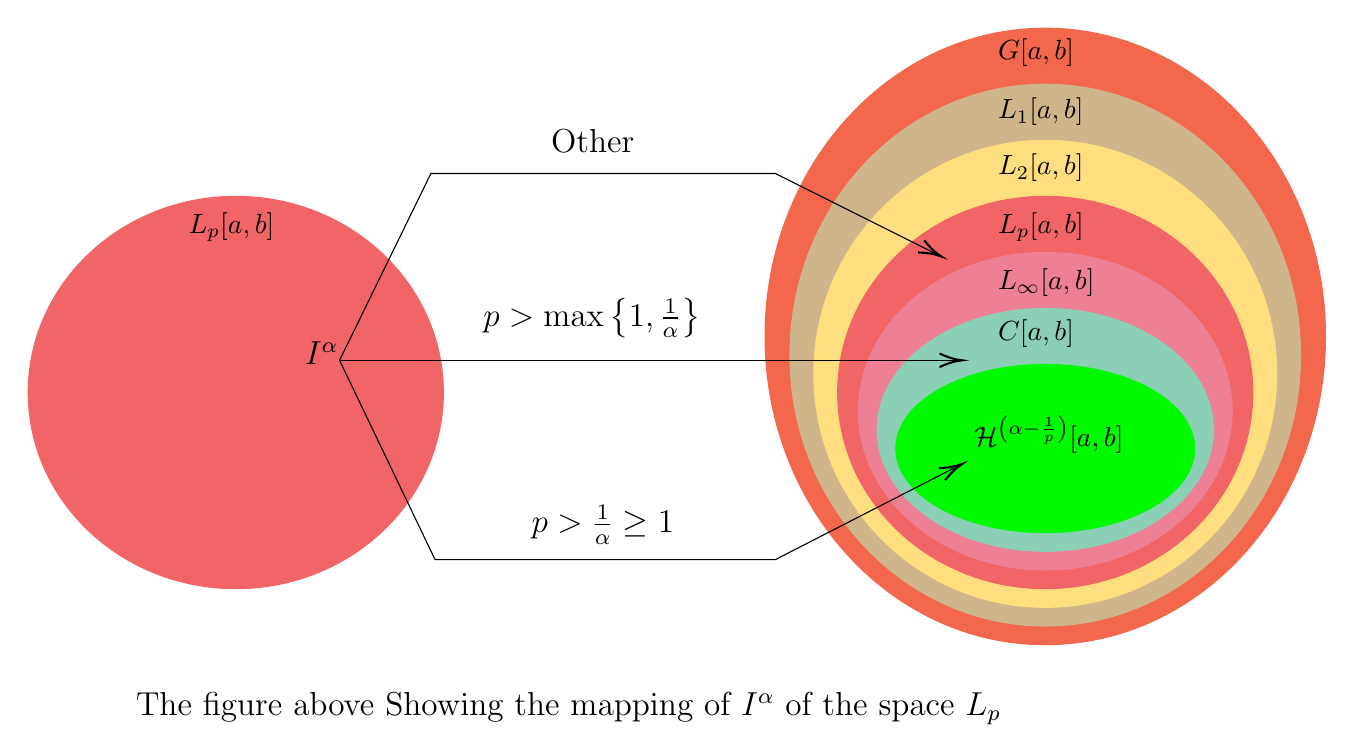
\begin{tikzpicture}[x=0.75pt,y=0.75pt,yscale=-1,xscale=1]
%uncomment if require: \path (0,757); %set diagram left start at 0, and has height of 757

%Shape: Ellipse [id:dp6907968999100429] 
\draw  [color={rgb, 255:red, 243; green, 103; blue, 77 }  ,draw opacity=1 ][fill={rgb, 255:red, 243; green, 103; blue, 77 }  ,fill opacity=1 ] (373.67,179.83) .. controls (373.67,97.82) and (434.11,31.33) .. (508.67,31.33) .. controls (583.23,31.33) and (643.67,97.82) .. (643.67,179.83) .. controls (643.67,261.85) and (583.23,328.33) .. (508.67,328.33) .. controls (434.11,328.33) and (373.67,261.85) .. (373.67,179.83) -- cycle ;
%Shape: Ellipse [id:dp455515408646161] 
\draw  [color={rgb, 255:red, 206; green, 182; blue, 138 }  ,draw opacity=1 ][fill={rgb, 255:red, 206; green, 182; blue, 138 }  ,fill opacity=1 ] (385.67,188.83) .. controls (385.67,116.76) and (440.74,58.33) .. (508.67,58.33) .. controls (576.6,58.33) and (631.67,116.76) .. (631.67,188.83) .. controls (631.67,260.91) and (576.6,319.33) .. (508.67,319.33) .. controls (440.74,319.33) and (385.67,260.91) .. (385.67,188.83) -- cycle ;
%Shape: Ellipse [id:dp45153781390969505] 
\draw  [color={rgb, 255:red, 255; green, 222; blue, 128 }  ,draw opacity=1 ][fill={rgb, 255:red, 255; green, 222; blue, 128 }  ,fill opacity=1 ] (397.17,197.83) .. controls (397.17,135.7) and (447.09,85.33) .. (508.67,85.33) .. controls (570.25,85.33) and (620.17,135.7) .. (620.17,197.83) .. controls (620.17,259.97) and (570.25,310.33) .. (508.67,310.33) .. controls (447.09,310.33) and (397.17,259.97) .. (397.17,197.83) -- cycle ;
%Shape: Ellipse [id:dp8046475401901105] 
\draw  [color={rgb, 255:red, 241; green, 101; blue, 103 }  ,draw opacity=1 ][fill={rgb, 255:red, 241; green, 101; blue, 103 }  ,fill opacity=1 ] (408.67,206.83) .. controls (408.67,154.64) and (453.44,112.33) .. (508.67,112.33) .. controls (563.9,112.33) and (608.67,154.64) .. (608.67,206.83) .. controls (608.67,259.02) and (563.9,301.33) .. (508.67,301.33) .. controls (453.44,301.33) and (408.67,259.02) .. (408.67,206.83) -- cycle ;
%Shape: Ellipse [id:dp6747974245031674] 
\draw  [color={rgb, 255:red, 238; green, 128; blue, 149 }  ,draw opacity=1 ][fill={rgb, 255:red, 238; green, 128; blue, 149 }  ,fill opacity=1 ] (418.67,215.83) .. controls (418.67,173.58) and (458.96,139.33) .. (508.67,139.33) .. controls (558.37,139.33) and (598.67,173.58) .. (598.67,215.83) .. controls (598.67,258.08) and (558.37,292.33) .. (508.67,292.33) .. controls (458.96,292.33) and (418.67,258.08) .. (418.67,215.83) -- cycle ;
%Shape: Ellipse [id:dp688684203224146] 
\draw  [color={rgb, 255:red, 139; green, 207; blue, 182 }  ,draw opacity=1 ][fill={rgb, 255:red, 139; green, 207; blue, 182 }  ,fill opacity=1 ] (427.67,224.83) .. controls (427.67,192.52) and (463.93,166.33) .. (508.67,166.33) .. controls (553.4,166.33) and (589.67,192.52) .. (589.67,224.83) .. controls (589.67,257.14) and (553.4,283.33) .. (508.67,283.33) .. controls (463.93,283.33) and (427.67,257.14) .. (427.67,224.83) -- cycle ;
%Shape: Ellipse [id:dp729097086157769] 
\draw  [color={rgb, 255:red, 0; green, 250; blue, 0 }  ,draw opacity=1 ][fill={rgb, 255:red, 0; green, 250; blue, 0 }  ,fill opacity=1 ] (436.67,233.83) .. controls (436.67,211.47) and (468.9,193.33) .. (508.67,193.33) .. controls (548.43,193.33) and (580.67,211.47) .. (580.67,233.83) .. controls (580.67,256.2) and (548.43,274.33) .. (508.67,274.33) .. controls (468.9,274.33) and (436.67,256.2) .. (436.67,233.83) -- cycle ;

%Shape: Ellipse [id:dp014732081794362362] 
\draw  [color={rgb, 255:red, 241; green, 101; blue, 103 }  ,draw opacity=1 ][fill={rgb, 255:red, 241; green, 101; blue, 103 }  ,fill opacity=1 ] (18.67,206.83) .. controls (18.67,154.64) and (63.44,112.33) .. (118.67,112.33) .. controls (173.9,112.33) and (218.67,154.64) .. (218.67,206.83) .. controls (218.67,259.02) and (173.9,301.33) .. (118.67,301.33) .. controls (63.44,301.33) and (18.67,259.02) .. (18.67,206.83) -- cycle ;
%Straight Lines [id:da35032145832073125] 
\draw    (168.67,191.33) -- (212.67,101.33) -- (378.67,101.33) -- (456.88,140.44) ;
\draw [shift={(458.67,141.33)}, rotate = 206.57] [color={rgb, 255:red, 0; green, 0; blue, 0 }  ][line width=0.75]    (10.93,-3.29) .. controls (6.95,-1.4) and (3.31,-0.3) .. (0,0) .. controls (3.31,0.3) and (6.95,1.4) .. (10.93,3.29)   ;
%Straight Lines [id:da6570360584697525] 
\draw    (168.67,191.33) -- (466.67,191.33) ;
\draw [shift={(468.67,191.33)}, rotate = 180] [color={rgb, 255:red, 0; green, 0; blue, 0 }  ][line width=0.75]    (10.93,-3.29) .. controls (6.95,-1.4) and (3.31,-0.3) .. (0,0) .. controls (3.31,0.3) and (6.95,1.4) .. (10.93,3.29)   ;
%Straight Lines [id:da6760674585190951] 
\draw    (168.67,191.33) -- (214.67,287.33) -- (378.67,287.33) -- (466.89,242.13) ;
\draw [shift={(468.67,241.22)}, rotate = 152.87] [color={rgb, 255:red, 0; green, 0; blue, 0 }  ][line width=0.75]    (10.93,-3.29) .. controls (6.95,-1.4) and (3.31,-0.3) .. (0,0) .. controls (3.31,0.3) and (6.95,1.4) .. (10.93,3.29)   ;

% Text Node
\draw (94.67,118.73) node [anchor=north west][inner sep=0.75pt]    {$L_{p}[ a,b]$};
% Text Node
\draw (484.67,35.23) node [anchor=north west][inner sep=0.75pt]    {$G[ a,b]$};
% Text Node
\draw (484.67,63.73) node [anchor=north west][inner sep=0.75pt]    {$L_{1}[ a,b]$};
% Text Node
\draw (484.67,90.73) node [anchor=north west][inner sep=0.75pt]    {$L_{2}[ a,b]$};
% Text Node
\draw (484.67,145.73) node [anchor=north west][inner sep=0.75pt]    {$L_{\infty }[ a,b]$};
% Text Node
\draw (484.67,118.73) node [anchor=north west][inner sep=0.75pt]    {$L_{p}[ a,b]$};
% Text Node
\draw (484.67,170.73) node [anchor=north west][inner sep=0.75pt]    {$C[ a,b]$};
% Text Node
\draw (473.17,216.73) node [anchor=north west][inner sep=0.75pt]    {$\mathcal{H}^{\left( \alpha -\frac{1}{p}\right)}[ a,b]$};
% Text Node
\draw (236.67,160) node [anchor=north west][font=\large,inner sep=0.75pt]    {$p >\max\left\{1,\frac{1}{\alpha }\right\}$};
% Text Node
\draw (260,260) node [anchor=north west][font=\large,inner sep=0.75pt]    {$p >\frac{1}{\alpha} \geq 1$};
% Text Node
\draw (150.67,180.96) node [anchor=north west][font=\large,inner sep=0.75pt]    {$I^{\alpha }$};
% Text Node
\draw (269.33,79) node [anchor=north west][font=\large,inner sep=0.75pt]   [align=left] {Other};
\draw (69.33,350) node [anchor=north west][font=\large,inner sep=0.75pt]   [align=left] {The figure above Showing the mapping of $I^{\alpha}$ of the space $L_p$};
\end{tikzpicture}
% }
\end{center}
% Where
% \begin{itemize}
%     \item $G(a,b)$ the space of all bounded functions on $[a,b]$
%     \item $L_1[a,b]$ the space of absolutely integrable functions on $[a,b]$
%     \[
%         \int_{a}^{b} f(t) dt < \infty \implies f(t) \in L_1[a,b]
%     \]
%     \item $L_2[a,b]$ also known as Hilbert space, the space of square-integrable functions on $[a,b]$
%     \[
%         \left( \int_{a}^{b} \left( f(t) \right)^2 dt \right)^{\frac{1}{2}} < \infty \implies f(t) \in L_2[a,b]
%     \]
%     \item $L_p[a,b]$ the space of p-integrable functions on $[a,b]$
%     \[
%         \left( \int_{a}^{b} \left( f(t) \right)^p dt \right)^{\frac{1}{p}} < \infty \implies f(t) \in L_p[a,b]
%     \]
%     \item $L_\infty[a,b]$ the space of essentially bounded measurable functions on $[a,b]$
%     \item $C[a,b]$ the space of continuous functions on $[a,b]$
%     \item $\mathcal{H}^{\lambda}[a,b]$ the space of Holderian functions of order $\lambda$ on $[a,b]$
% \end{itemize}

% \[
%     G(a,b) \supset  L_1[a,b] \supset L_2[a,b] \supset L_p[a,b]  \supset L_\infty[a,b] \supset C[a,b] \supset \mathcal{H}^{\lambda}[a,b]
% \]             % Integration Part 
\section{Fractional Differentiation}

One might assume that fractional differentiation can be 
accomplished by assuming that $\displaystyle \dv[n]{}{x} = I^{-n} $
but this doesn't work because the gamma doesn't 
actually extend to ALL the real numbers. 
\\
Gamma is actually undefined for non-positive integer inputs, 
so we wouldn't be able to plug in $n = -1$ into gamma to compute 
a derivative using the Fractional Integral formula (2.3).
\\
But even for fractional negative orders like $\displaystyle \alpha = -\frac{1}{2}$,
it turns out the integral expression becomes 
divergent, since an integral of the form $\displaystyle t^{(\alpha-1)}$ is divergent 
near $t = 0$ for non-positive values of $\alpha$

\subsection{Riemann-Liouville Fractional Derivative}
We know that from classical calculus integer order derivatives 
and integrals they're supposed to be inverses of each other, 
and should cancel each other out.

i.e $\forall n > 0 , n \in \mathbb{Z}^+$ the $ n^{\text{th}} $ derivative of the $ n^{\text{th}} $ integral 
is the function itself (The First Fundamental Theorem of Calculus)
\[
    \dv[n]{}{t} I^{n} f(t) = f(t)    
\]

So we can use this formula indirectly to compute a half-derivative 
by say first compute a half-integral and then taking the 
ordinary whole derivative of that 

Basically using the fractional integral to get us some kind 
of fractional order then using ordinary derivatives to sort 
of "lower" that order to where we actually want it. 

This technique is called the Riemann-Liouville fractional derivative
\vspace*{.2cm}
\begin{definition}[Riemann-Liouville Fractional Derivative]
    Let $\alpha>0$ for a positive integer $m$ such that $\alpha \in [m-1,m]$ we define the Riemann-Liouville 
    fractional derivative of order $\alpha$ by 
    \begin{equation}
        D^{\alpha} f(t) = \dv[m]{}{t} I^{m-\alpha} f(t)
    \end{equation}
    And by using the Riemann-Liouville fractional integration formula (2.3) we can 
    rewrite a formula for the fractional derivative as follows 
    \begin{equation}
        D^{\alpha} f(t) =  \frac{1}{\Gamma(m-\alpha)} \dv[m]{}{t}\int_{0}^{t} (t-s)^{m - \alpha -1} \hquad f(s) \hquad ds
    \end{equation}
    When $\alpha$ is equal to 0.5 we call this a semi-derivative 
\end{definition}
\begin{example}
    Evaluate $D^{\alpha}(f(t))$ where $f(t) = t^n$ , $n>-1$

    \textit{ \textbf{Sol.} }
    \begin{align*}
        D^{\alpha} (t^n) &=  \dv[m]{}{t}\left( I^{m-\alpha} (t^n) \right)
        \intertext{And we know that}
        I^{m-\alpha} (t^n) &=  \left[t^{n+\alpha}\frac{\Gamma{(n+1)} } {\Gamma{(n+\alpha+1)} }\right]_{\alpha = m-\alpha}
        \\
        \therefore \dv[m]{}{t}\left( t^{n+m-\alpha}\frac{\Gamma{(n+1)} } {\Gamma{(n+1+m-\alpha)} } \right) &=  \frac{\Gamma{(n+1)} } {\Gamma{(n+1+m-\alpha)} }  \dv[m]{}{t}t^{n+m-\alpha}
        \\
        &=  \frac{\Gamma{(n+1)} } {\Gamma{(n+1+m-\alpha)} }  \frac{\Gamma{(n+1+m-\alpha)} }{\Gamma{(n+1+m-\alpha-m)} }  t^{n-\alpha}
        \\
        &= t^{n-\alpha}\frac{\Gamma{(n+1)} } {\Gamma{(n-\alpha+1)} }
    \end{align*}
\end{example}
\begin{example}
    Evaluate $D^{\alpha}(t^n)$ when $n=\alpha$ and when $n=\alpha-k$ for $k=1,2,3,\dots$

    \textit{ \textbf{Sol.} }
    \[
        D^{\alpha} (t^n) =  t^{n-\alpha}\frac{\Gamma{(n+1)} } {\Gamma{(n-\alpha+1)} }    
    \]
    At $n=\alpha$
    \[
        D^{\alpha} (t^\alpha) =  t^{\alpha-\alpha}\frac{\Gamma(\alpha+1) } {\Gamma{(\alpha-\alpha+1)} } = \Gamma(\alpha+1)
    \]
    At $n=\alpha-k$
    \[
        D^{\alpha} (t^{\alpha-k}) =  t^{\alpha-k-\alpha}\frac{\Gamma(\alpha-k+1) } {\Gamma{(\alpha-k-\alpha+1)} } = \frac{\Gamma(\alpha-k+1) } {t^k\Gamma{(1-k)}}
    \]
    We know that $\Gamma(x)$ maps non-positive integer numbers to $\{\infty,-\infty\}$ 
    
    Thus for $k=1,2,3,\dots,m-1$
    \begin{equation}
        D^{\alpha} (t^{\alpha-k}) = 0
    \end{equation}
    That for $k<m$ to make sure that $\Gamma(\alpha-k+1)$ is not $\{\infty,-\infty\}$ 
\end{example}
\subsection{Caputo Fractional Derivative}
\begin{figure*}[b]
    \begin{minipage}[h]{\textwidth}
        \begin{enrichment}{Michele Caputo}{Chars/Caputo.jpg}{2.4}{.8}{.17}
            Professor Michele Caputo is a distinguished mathematician known for his contributions to the field of 
            fractional calculus, particularly his creation of the Caputo derivative$.$ 
            His work has significantly advanced 
            our understanding of fractional calculus and its applications$.$
            With a career marked by innovation and scholarly excellence, 
            Caputo has established himself as a leading authority in the mathematical community
        \end{enrichment} 
    \end{minipage}
\end{figure*}
Someone might say instead of taking the fractional integral of order $m-\alpha$ for a function then differentiate it $m-times$
we can differentiate it $m-times$ first then taking the fractional integral of order $m-\alpha$ for it 
\\
This what Prof$.$ Michele Caputo did in 1967 when he introduced
the Caputo fractional derivative definition
but this alternative definition doesn't always give the same results as the original
\vspace*{.2cm}
\begin{definition}[Caputo Fractional Derivative]
    Let $\alpha>0 \quad,\quad m-1<\alpha<m$ , $m \in \mathbb{N}^+ $ Caputo Fractional Derivative is defined by    
    \begin{equation}
        \leftindex[I]^C{D^\alpha} f(t) = I^{m-\alpha} \dv[m]{}{t} f(t) =  \frac{1}{\Gamma(m-\alpha)} \int_{0}^{t} (t-s)^{m - \alpha -1}\dv[m]{f(s)}{s} \hquad ds
    \end{equation}
\end{definition}
\begin{example}
    Evaluate $D^{\alpha}(f(t))$ where $f(t) = t^n$ and $n>m-1 \quad,\quad n \in \mathbb{R}$
    
    \textit{ \textbf{Sol.} }
    \begin{align*}
        \leftindex[I]^C {D^{\alpha}} (t^n) &=  I^{m-\alpha}\left[\dv[m]{}{t} t^n \right] =  I^{m-\alpha} \left[ t^{n-m}\frac{\Gamma{(n+1)} } {\Gamma{(n-m+1)} } \right]
        \\
        &=  \frac{\Gamma{(n+1)} } {\Gamma{(n-m+1)} } \left[ \frac{\Gamma{(n-m+1)}}{\Gamma{(n+1-m+m-\alpha)} } t^{n-m+m-\alpha} \right]
        \\
        &=  \frac{\Gamma{(n+1)} }{\Gamma{(n+1-\alpha)} } t^{n-\alpha}
    \end{align*}
    If $n<m-1 \quad,\quad n \in \mathbb{N}$
    \begin{equation}
        \leftindex[I]^C {D^{\alpha}} (t^n) =  I^{m-\alpha}\left[\dv[m]{}{t} t^n \right]=  I^{m-\alpha}\left[0\right]=0    
    \end{equation}
\end{example}
\subsection{The Differences And Properties Of Riemann-Liouville And Caputo Derivative}
\textcolor{theme}{1.}\textbf{ Restrictions On The Order}

\textcolor{blue}{In Riemann-Liouville} For $\alpha \in [m-1,m]$ , $m$ can be any positive natural number we are not restricted to make it small as possible
\[
    D^{\frac{1}{2}} f(t) = \dv{}{t} I^{\frac{1}{2}} f(t) = \dv[5]{}{t} I^{4.5} f(t) =  D^{4.5} f(t) = D^{8.5} f(t) = \dots
\]
That's due to the (semi-group) property of the fractional integral
\[
            \dv[5]{}{t} I^{4.5} f(t)= \dv[5]{}{t} I^{4}I^{\frac{1}{2}} f(t)= \dv{}{t} I^{\frac{1}{2}} f(t) = D^{\frac{1}{2}} f(t) 
\]
\textcolor{orange}{In Caputo} This is not true with Caputo 
\[
    \leftindex[I]^C {D^{\frac{1}{2}}} f(t) =  I^{\frac{1}{2}} \dv{}{t} f(t) \neq I^{4.5} \dv[5]{}{t} f(t) \neq I^{8.5} \dv[9]{}{t} f(t)
\]
To show that let $f(t) = t^2$
\[
    \leftindex[I]^C {D^{\frac{1}{2}}} t^2 = I^{\frac{1}{2}} \dv{}{t} t^2 = I^{\frac{1}{2}} 2t
\]
\[
    \leftindex[I]^C {D^{\frac{1}{2}}} t^2 = I^{\frac{5}{2}} \dv[3]{}{t} t^2 = I^{\frac{5}{2}} 0 = 0
\]

\textcolor{theme}{2.}\textbf{ Restrictions On The Function}

\textcolor{blue}{In Riemann-Liouville} $f \in L_1[0,b]$ ((may exist even for some discontinuous functions))

\textcolor{orange}{In Caputo} $f$ is differentiable and $f' \in L_1[0,b]$ ((at least $f \in AC[0,b]$))
\begin{enrichment*}{Absolute Continuous Functions}
    A function $f$ is said to be Absolute Continuous i.e $f \in AC^{n}[0,b]$ if it's defined on $[0,b]$ and have continuous derivatives up to order $(n-1)$ on $[0, b]$
    and $f^{(n-1)}$ is absolutely continuous on $[0,b]$
\end{enrichment*}



\textcolor{theme}{3.}\textbf{ Linearity}

\textcolor{blue}{In Riemann-Liouville} Let $a,b$ be constants
\[
    D^{\alpha} [a \hquad f(t) + b \hquad g(t)] =  a \hquad D^{\alpha}f(t) + b \hquad D^{\alpha}g(t)
\]
\textcolor{orange}{In Caputo} Let $a,b$ be constants
\[
    \leftindex[I]^C {D^{\alpha}} [a \hquad f(t) + b \hquad g(t)] =  a \hquad \leftindex[I]^C {D^{\alpha}} f(t) + b \hquad\leftindex[I]^C {D^{\alpha}} g(t)
\]
\textcolor{theme}{4.}\textbf{ Effect On Constant}

\textcolor{blue}{In Riemann-Liouville}
    \[
        D^{\alpha} c = \frac{t^{-\alpha}}{\Gamma{(1-\alpha)} }
    \]
\textcolor{orange}{In Caputo} 
    \[
            \leftindex[I]^C {D^{\alpha}} c = I^{m-\alpha}\left[\dv[m]{}{t} c \right] = I^{m-\alpha}\left[0\right] = 0
    \]
    Which is most important difference between RL and Caputo and it consider an advantage for Caputo over RL and show us that 
    \[
        \leftindex[I]^C {D^{\alpha}} f(t) \neq D^{\alpha} f(t)
    \]
\newpage
\textcolor{theme}{5.}\textbf{ Continuity With Respect To The Order Of Derivation}

We naturally expect that $D_a^{\alpha} f(t)$ and $\leftindex[I]^C {D_a^{\alpha}} f(t)$ to be a continuous functions. It is clear that complications 
may occur only at points which represent the integer-order derivatives. 

Let $m-1 < \alpha < m$ and $f(t)$ has a sufficient number of continuous derivatives.

\textcolor{blue}{In Riemann-Liouville}
\begin{align*}
    \lim_{\alpha \to m }D_a^{\alpha} f(t) &=  \lim_{\alpha \to m } \left\{\frac{1}{\Gamma(m-\alpha)} \dv[m]{}{t}\int_{a}^{t} (t-s)^{m - \alpha -1} \hquad f(s) \hquad ds    \right\}
    \\
    \intertext{Integrate by part $(m+1)-times$}
    &=  \lim_{\alpha \to m } \dv[m]{}{t} \left[ \sum_{k=0}^{m}  \frac{(t-a)^{m+k-\alpha}f^{(k)}(a)}{\Gamma(m+k+1-\alpha)}
    + \int_{a}^{t} \frac{(t-s)^{2m - \alpha}}{\Gamma(2m-\alpha+1)} \hquad f^{(m+1)}(s) \hquad ds\right]
    \\
    &=  \lim_{\alpha \to m } \left[ \sum_{k=0}^{m} \frac{(t-a)^{k-\alpha}f^{(k)}(a)}{\Gamma(k+1-\alpha)} 
    + \int_{a}^{t} \frac{(t-s)^{m - \alpha}}{\Gamma(m-\alpha+1)} \hquad f^{(m+1)}(s) \hquad ds\right]
    \intertext{All the summation terms except the last one will be zero due to the Gamma in the denominator which will be $\{-\infty,\infty\}$ when $\alpha$ is replaced by $m$}
    &= f^{(m)}(a) + \int_{a}^{t} f^{(m+1)}(s) \hquad ds
    \\
    &= f^{(m)}(a) + f^{(m)}(t) - f^{(m)}(a) = f^{(m)}(t)
\end{align*}
This does not hold for points of the discontinuity of some derivative involved.

\textcolor{orange}{In Caputo} 

The calculation of the left limit is similar and even more easier
\begin{align*}
    \lim_{\alpha \to m^- } \leftindex[I]^C {D_a^{\alpha}} f(t) &=  \lim_{\alpha \to m^- } \left\{\frac{1}{\Gamma(m-\alpha)} \int_{a}^{t} (t-s)^{m - \alpha -1} \hquad f^{(m)}(s) \hquad ds    \right\}
    \\
    \intertext{Integrate by part}
    &=  \lim_{\alpha \to m^- } \left[ \frac{(t-a)^{m-\alpha}f^{(m)}(a)}{\Gamma(m+1-\alpha)} 
    + \int_{a}^{t} \frac{(t-s)^{m - \alpha}}{\Gamma(m-\alpha+1)} \hquad f^{(m+1)}(s) \hquad ds\right]
    \\
    &= f^{(m)}(a) + \int_{a}^{t} f^{(m+1)}(s) \hquad ds = f^{(m)}(t)
\end{align*}
The right limit for the Caputo derivative is as follows
\[
    \lim_{\alpha \to (m-1)^+ } \leftindex[I]^C {D_a^{\alpha}} f(t) =  \int_{a}^{t} f^{(m)}(s) \hquad ds = f^{(m-1)}(t) - f^{(m-1)}(a)
\]
This result destroys our hope in the continuity of the Caputo derivative with respect to $\alpha$. 
The function $f(t)$ would have to fulfill $f^{(m-1)}(a) = 0$ and it seems like a very strong restriction.
\\
But, most functions used in fractional calculus satisfy this condition so it is not such
a big complication.
\\
In addition we could expect this result because it coincides with one of the requirement
for the Caputo derivative the zero value of all derivatives of a constant function.
\newpage
\textcolor{theme}{6.}\textbf{ Equivalence Of The Approaches}

We impose $f(t)$ to be $(m-1)-times$ continuously differentiable and the $m^{\text{th}}$ derivative of $f(t)$ to be integrable. 
\\
We suppose as usual $\alpha > 0$, but $\alpha \neq m-1$
\begin{align*}
    D_a^\alpha f(t) &= \frac{1}{\Gamma(m-\alpha)} \dv[m]{}{t}\int_{a}^{t} (t-s)^{m - \alpha -1} \hquad f(s) \hquad ds
    \intertext{Integrate by part $m-times$}
    &= \dv[m]{}{t} \left[ \sum_{k=0}^{m-1}  \frac{(t-a)^{m+k-\alpha}f^{(k)}(a)}{\Gamma(m+k+1-\alpha)} 
    + \int_{a}^{t} \frac{(t-s)^{2m - \alpha-1}}{\Gamma(2m-\alpha)} \hquad f^{(m)}(s) \hquad ds\right]
    \\
    &= \sum_{k=0}^{m-1}  \frac{(t-a)^{k-\alpha}f^{(k)}(a)}{\Gamma(k+1-\alpha)} 
    + \int_{a}^{t} \frac{(t-s)^{m - \alpha-1}}{\Gamma(m-\alpha)} \hquad f^{(m)}(s) \hquad ds
    \\
    &= \sum_{k=0}^{m-1}  \frac{(t-a)^{k-\alpha}f^{(k)}(a)}{\Gamma(k+1-\alpha)} 
    + \leftindex[I]^C {D_{a}^{\alpha}} f(t)
\end{align*}
A more interesting situation occurs when $a \to -\infty$ because due to $k - \alpha < 0$ for all
$k$, the power functions are zero for all values $\alpha$ and we obtain
\[
    D_{-\infty}^\alpha f(t) = \leftindex[I]^C {D_{-\infty}^{\alpha}} f(t)
\]
\textcolor{theme}{7.}\textbf{ Equivalence Of Functions Derivatives}

\textcolor{blue}{In Riemann-Liouville}
    \[
        D^{\alpha} f(t) =  D^{\alpha} g(t) \Longleftrightarrow f(t) = g(t) + \sum_{k=1}^{m} C_k t^{\alpha-k}
    \]
\begin{proof}[Proof]
    Let 
    \begin{align*}
        f(t) &= g(t) + \sum_{k=1}^{m} C_k t^{\alpha-k}    
        \intertext{Take $D^{\alpha}$ for both sides}
        D^{\alpha} f(t) &= D^{\alpha} g(t) + D^{\alpha} \sum_{k=1}^{m} C_k t^{\alpha-k}    
        \\
        &= D^{\alpha} g(t) + \sum_{k=1}^{m} C_k D^{\alpha} t^{\alpha-k}    
        \intertext{From equation (3.3) we got that $D^{\alpha} t^{\alpha-k} = 0$ Thus }
        D^{\alpha} f(t) &=  D^{\alpha} g(t)
    \end{align*}
    Conversely let 
    \begin{align*}
        D^{\alpha} f(t) &=  D^{\alpha} g(t)
        \intertext{Take $I^{\alpha}$ for both sides}
        f(t) &=  g(t) + H(t)
        \\
        f(t) &=  g(t) + \sum_{k=1}^{m} C_k t^{\alpha-k}    
    \end{align*}
\end{proof}
\textcolor{orange}{In Caputo}
    \[
        \leftindex[I]^C {D^{\alpha}} f(t) =  \leftindex[I]^C {D^{\alpha}} g(t) \Longleftrightarrow f(t) = g(t) + \sum_{k=1}^{m} C_k t^{m-k}
    \]
\begin{proof}[Proof]
    Let 
    \begin{align*}
        f(t) &= g(t) + \sum_{k=1}^{m} C_k t^{m-k}    
        \intertext{Take $\leftindex[I]^C {D^{\alpha}}$ for both sides}
        \leftindex[I]^C {D^{\alpha}} f(t) &= \leftindex[I]^C {D^{\alpha}} g(t) + \leftindex[I]^C {D^{\alpha}} \sum_{k=1}^{m} C_k t^{\alpha-k}    
        \\
        &= \leftindex[I]^C {D^{\alpha}} g(t) + \sum_{k=1}^{m} C_k \leftindex[I]^C {D^{\alpha}} t^{m-k}    
        \intertext{From equation (3.5) we got that $\leftindex[I]^C {D^{\alpha}} t^{m-k} = 0$ Thus }
        \leftindex[I]^C {D^{\alpha}} f(t) &=  \leftindex[I]^C {D^{\alpha}} g(t)
    \end{align*}
    Conversely let 
    \begin{align*}
        \leftindex[I]^C {D^{\alpha}} f(t) &=  \leftindex[I]^C {D^{\alpha}} g(t)
        \intertext{Take $I^{\alpha}$ for both sides}
        f(t) &=  g(t) + H(t)
        \\
        f(t) &=  g(t) + \sum_{k=1}^{m} C_k t^{m-k}    
    \end{align*}
\end{proof}
\textcolor{theme}{8.}\textbf{ Effect Of Integer Derivative}

For $k = 0,1,2,\dots$

\textcolor{blue}{In Riemann-Liouville}
\begin{align*}
    \dv[k]{}{t} D^{\alpha} f(t) &=  \dv[k]{}{t} \dv[m]{}{t} I^{m-\alpha} f(t) 
    \\
    &= \dv[m+k]{}{t} I^{m-\alpha} f(t) 
    \\
    &= \dv[m+k]{}{t} I^{m+k-k-\alpha} f(t) = \dv[m+k]{}{t} I^{(m+k)-(\alpha+k)} f(t) 
    \\
    &= D^{\alpha+k} f(t)
\end{align*}
\textcolor{orange}{In Caputo} 
\begin{align*}
    \leftindex[I]^C {D^{\alpha}} \dv[k]{}{t}f(t) &= I^{m-\alpha}\dv[m]{}{t}\dv[k]{}{t} f(t) 
    \\
    &= I^{m-\alpha}\dv[m+k]{}{t} f(t) 
    \\
    &= I^{m+k-k-\alpha}\dv[m+k]{}{t} f(t) = I^{(m+k)-(\alpha+k)}\dv[m+k]{}{t} f(t) 
    \\
    &= \leftindex[I]^C {D^{\alpha+k}} f(t)
\end{align*}
\newpage

\textcolor{theme}{9.}\textbf{ The Integral Of Derivative}

\textcolor{orange}{In Caputo} 
\begin{align}
    \notag
    I^{\alpha}\leftindex[I]^C {D^{\alpha}}f(t) & = I^{\alpha}\left[\frac{1}{\Gamma(m-\alpha)}\int_{0}^{t}(t-s)^{m-\alpha-1}\dv[m]{}{s}f(s) \hquad ds\right]
    \\\notag
                             & = \frac{1}{\Gamma(\alpha)\Gamma(m-\alpha)} \int_{0}^{t}(t-s)^{\alpha-1} \int_{0}^{s}(s-\theta)^{m-\alpha-1} \dv[m]{}{\theta} f(\theta) \hquad d\theta \hquad ds
    \\
                             & = \frac{1}{\Gamma(\alpha)\Gamma(m-\alpha)} \int_{0}^{t}\underbrace{\int_{\theta}^{t}(t-s)^{\alpha-1}(s-\theta)^{m-\alpha-1} ds}_J  \dv[m]{}{\theta} f(\theta) \hquad d\theta
\end{align}
Let's handle the inner integral first
\begin{align*}
    J & = \int_{\theta}^{t}(t-s)^{\alpha-1}(s-\theta)^{m-\alpha-1} \hquad ds
    \intertext{
        Substitute
    \(
    \begin{cases}
        \displaystyle s-\theta = \eta
        \\\\
        \displaystyle ds = d\eta
        \\\\
        \displaystyle 0 \to t-\theta
    \end{cases}
    \)
    }
      & = \int_{0}^{t-\theta}(t-\theta-\eta)^{\alpha-1}(\eta)^{m-\alpha-1} \hquad d\eta
    \\
      & = (t-\theta)^{\alpha-1} \int_{0}^{t-\theta}(1-\frac{\eta}{t-\theta})^{\alpha-1}(\eta)^{m-\alpha-1} \hquad d\eta
    \intertext{
        Substitute
    \(
    \begin{cases}
        \displaystyle \eta = (t-\theta)\xi
        \\\\
        \displaystyle d\eta = (t-\theta) \hquad d\xi
        \\\\
        \displaystyle 0 \to 1
    \end{cases}
    \)
    }
      & = (t-\theta)^{\alpha-1} \int_{0}^{1}(1-\xi)^{\alpha-1} (t-\theta)^{m-\alpha-1} \hquad \xi^{m-\alpha-1} \hquad (t-\theta)  \hquad  d\xi
    \\
      & = (t-\theta)^{\alpha+m-\alpha-1} \int_{0}^{1}(1-\xi)^{\alpha-1} \hquad \xi^{m-\alpha-1} \hquad d\xi 
    \\
      & = (t-\theta)^{m-1} \beta(\alpha,m-\alpha)
\end{align*}
Substitute in (3.6) we get that
\begin{align*}
    I^{\alpha}\leftindex[I]^C {D^{\alpha}} f(t) &= \frac{\beta(\alpha,m-\alpha)}{\Gamma(\alpha)\Gamma(m-\alpha)}\int_{0}^{t} (t-\theta)^{m-1} \dv[m]{}{\theta} f(\theta) \hquad d\theta
    \\
    &= \frac{1}{\Gamma(m)}\int_{0}^{t} (t-\theta)^{m-1} \dv[m]{}{\theta} f(\theta) \hquad d\theta
    \intertext{Integrate by part $(m-1)-times$}
    &= f(t) - \sum_{k=0}^{m-1}  \frac{t^{m-k-1}f^{(m-k-1)}(0)}{\Gamma(m-k)} 
    \intertext{If we put $k = m-k-1$ the summation value will not change only it's order}
    &= f(t) - \sum_{k=0}^{m-1}  \frac{t^{k}f^{(k)}(0)}{\Gamma(k+1)}  = f(t) - \sum_{k=0}^{m-1}  \frac{t^{k}}{k!}f^{(k)}(0)
\end{align*}

\textcolor{blue}{In Riemann-Liouville} 
\\
Using the Equivalence Of The Approaches relation
\begin{align*}
    I^{\alpha}D^{\alpha} f(t) &= I^{\alpha} \left[ \sum_{k=0}^{m-1}  \frac{t^{k-\alpha}f^{(k)}(0)}{\Gamma(k+1-\alpha)} + \leftindex[I]^C {D^{\alpha}} f(t) \right]
    \\
    &= \sum_{k=0}^{m-1}  \frac{f^{(k)}(0)}{\Gamma(k+1-\alpha)}I^{\alpha}t^{k-\alpha} + I^{\alpha}\leftindex[I]^C {D^{\alpha}} f(t)
    \\
    &= \sum_{k=0}^{m-1}  \frac{f^{(k)}(0)}{\Gamma(k+1-\alpha)}t^k \frac{\Gamma(k+1-\alpha)}{\Gamma(k+1)} + f(t) - \sum_{k=0}^{m-1}  \frac{t^{k}}{k!}f^{(k)}(0)
    \\
    &= \sum_{k=0}^{m-1}  \frac{t^{k}}{k!}f^{(k)}(0) + f(t) - \sum_{k=0}^{m-1}  \frac{t^{k}}{k!}f^{(k)}(0) = f(t)
\end{align*}

\textcolor{theme}{10.}\textbf{ The Interchange Of The Differentiation Operators}

\textcolor{blue}{In Riemann-Liouville}
\[
    D_a^{k}\left(D_a^{\alpha} f(t)\right) = D_a^{\alpha} \left(D_a^{k} f(t)\right) = D_a^{\alpha+k} f(t)
\]
Is allowed under the conditions
\[
    f^{(i)}(a)=0 \quad,\quad i=0,1,2,\dots,k \quad,\quad k=0,1,2,\dots \quad,\quad m-1<\alpha<m
\]
\textcolor{orange}{In Caputo} 
\[
    \leftindex[I]^C {D_a^{k}} \left(\leftindex[I]^C {D_a^{\alpha}} f(t)\right) = 
    \leftindex[I]^C {D_a^{\alpha}} \left(\leftindex[I]^C {D_a^{k}} f(t)\right) =
    \leftindex[I]^C {D_a^{\alpha+k}} f(t)
\]
Is allowed under the conditions
\[
    f^{(i)}(a)=0 \quad,\quad i=m,m+1,\dots,k \quad,\quad k=0,1,2,\dots \quad,\quad m-1<\alpha<m
\]
Contrary to the RL approach in the case of the Caputo derivative there are no restrictions on the values 
$f^{(i)}(a)$ for $i=0,1,2,\dots,m-1$

\newpage
\textcolor{theme}{11.}\textbf{ Non-Locality}

Normally when we take first or second 
derivatives the output of the derivative only depends on the 
input we give it this is called locality i.e. $f^{(n)}(t)$
only depends on $t$. now if we go back to the definition of a fractional derivative we 
have constant $a$ at the bottom of the integral 
\[
    D_{a}^{\alpha} f(t) = \frac{1}{\Gamma(m-\alpha)} \dv[m]{}{t}\int_{\textcolor{red}{\fbox{\textcolor{black}{$a$}}}}^{t} (t-s)^{m - \alpha -1} \hquad f(s) \hquad ds
\]
Thus the fractional derivative has Non-locality which means 
that it's value at a point depends on the function values over an interval, 
not just at that point.
\\
The next two examples will show the effect of this property
\vspace*{-.4cm}
\begin{example}
    Evaluate $\displaystyle D_{0}^{\alpha} (E_{a,b}(\lambda t))$

    \textit{ \textbf{Sol.} }
    \begin{equation}
        D_{0}^{\alpha} (E_{a,b}(\lambda t)) = D_{0}^{\alpha} \left(\sum_{k=0}^{\infty}\frac{{(\lambda t)}^k}{\Gamma(a k + b )}\right)
    \end{equation}
    Because the series in (3.7) is uniformly convergent we can interchange $D_{0}^{\alpha}$ with the summation
    \[
        D_{0}^{\alpha} (E_{a,b}(\lambda t)) = \sum_{k=0}^{\infty}\frac{D_{0}^{\alpha} ((\lambda t)^k)}{\Gamma(a k + b )} = \sum_{k=0}^{\infty}\frac{\lambda^k D_{0}^{\alpha} (t^k)}{\Gamma(a k + b )}
    \]
    And we know that 
    \[
        D_{0}^{\alpha} (t^n) = t^{n-\alpha}\frac{\Gamma{(n+1)} } {\Gamma{(n-\alpha+1)} }    
    \]
    Thus 
    \[
        D_{0}^{\alpha} (E_{a,b}(\lambda t)) = \sum_{k=0}^{\infty}\frac{\Gamma{(k+1)} } {\Gamma{(k-\alpha+1)} } \frac{(\lambda^k t^{k-\alpha})}{\Gamma(a k + b )} = t^{-\alpha} \sum_{k=0}^{\infty}\frac{\Gamma{(k+1)} } {\Gamma{(k-\alpha+1)} } \frac{({\lambda t})^k}{\Gamma(a k + b )}
    \]
    At $a,b = 1$ 
    \begin{align*}
        D_{0}^{\alpha} (E_{1,1}(\lambda t)) = D_{0}^{\alpha} (e^{\lambda t}) &= t^{-\alpha} \sum_{k=0}^{\infty}\frac{\Gamma{(k+1)} } {\Gamma{(k-\alpha+1)} } \frac{(\lambda t)^{k}}{\Gamma(k + 1 )}
        \\
        & = t^{-\alpha} \sum_{k=0}^{\infty} \frac{((\lambda t)^{k})}{\Gamma(k+1-\alpha)} = t^{-\alpha} (E_{1,1-\alpha}(\lambda t))
    \end{align*}
\end{example}
\vspace*{-.6cm}
\begin{example}
    Evaluate $\displaystyle D_{-\infty}^{\alpha} (e^{\lambda t})$
    
    \textit{ \textbf{Sol.} }
    \begin{align*}
        D_{-\infty}^{\alpha} (e^{\lambda t}) &=  \frac{1}{\Gamma(m-\alpha)} \dv[m]{}{t}\int_{-\infty}^{t} (t-s)^{m - \alpha -1}(e^{\lambda s}) \hquad ds    
        \intertext{
            Substitute
    \(
    \begin{cases}
        \displaystyle \frac{\xi}{\lambda} = (t-s)
        \\
        \displaystyle d\xi = -\lambda \hquad ds
        \\
        \displaystyle \infty \to 0
    \end{cases}
    \)
        }
        &=  \frac{1}{\Gamma(m-\alpha)} \dv[m]{}{t}\int_{\infty}^{0} \left(\frac{\xi}{\lambda}\right)^{m - \alpha -1}(e^{\lambda t - \xi}) \left(-\frac{1}{\lambda}\right) \hquad d\xi    
        \\
        &=\frac{1}{\Gamma(m-\alpha)} \dv[m]{}{t} \left(\frac{1}{\lambda}\right)^{m - \alpha} e^{\lambda t} \int_{0}^{\infty} \xi^{m - \alpha -1}(e^{- \xi}) \hquad d\xi    
        \\
        &=\frac{\lambda^{\alpha-m}}{\Gamma(m-\alpha)} \dv[m]{}{t} e^{\lambda t} \hquad \Gamma(m-\alpha)
        \\
        &=\lambda^{\alpha-m} \lambda^{m} e^{\lambda t} = \lambda^{\alpha} e^{\lambda t}
    \end{align*}
\end{example}

Advantages Of Nonlocality:
\begin{enumerate}
    \item Modeling Complex Phenomena : Fractional derivatives are useful Analyzing functions that not only depend on time for example some phenomenon in the real world have something called a memory effect which means that the current state not only depends on time but also in previous States Many physical systems exhibit such behaviors, including viscoelastic materials, anomalous diffusion, and certain types of signal processing. traditional differential equations have a hard time modeling phenomenon like this but fractional derivatives can make the task easier 
    \item Anomalous Diffusion : They are also useful for describing anomalous diffusion phenomena, where the mean squared displacement of particles does not follow a linear relationship with time. Such phenomena are prevalent in complex systems like porous media, biological tissues, and turbulent flows.
\end{enumerate}

Disadvantages Of Nonlocality:
\begin{enumerate}
    \item Computational Challenges : Numerical approximation and computation of fractional derivatives can be computationally intensive and require specialized algorithms. This can pose challenges, especially when dealing with large-scale systems or real-time applications.
    \item Interpretation Difficulty : Non-locality introduced by fractional derivatives can sometimes make it difficult to interpret the physical meaning of the derived equations. Understanding the behavior of systems described by fractional calculus may require a deeper conceptual grasp compared to classical systems.
\end{enumerate}

This raises the question of how exactly we can interpret fractional derivatives. 
since they're non-local and are influenced by the function's behavior far away 
from a given input point, they must represent something different 
than the slope of a tangent line, which is all about measuring a 
function's local behavior near a point.

Despite ordinary derivatives and integrals having pretty 
straightforward geometric and physical meanings, it seems no one 
has come up with a truly satisfying, general interpretation of 
the fractional operators, or at least not one that's widely 
accepted.

Trying too hard to interpret fractional calculus in 
terms of ordinary calculus is probably like insisting on 
interpreting the equation $\displaystyle e^{i\pi} = -1$ in terms 
of repeated multiplication. $\underbrace{ee \dots ee}_{i\pi \hquad  times} = -1$

Note that some familiar properties \textcolor{red}{Don't Work Anymore}

\textcolor{red}{12.}\textbf{ The Chain Rule}
\[
    D f(g(t)) = f'(g(t))g'(t)
\]
\begin{proof}[Proof]
    counter-example let $g(t) = t^2$ and $f(g)=g^2$ 
    \\
    If we use the chain rule
    \[
        D^\alpha f(g(t)) = D^\alpha g(t)^2 = g(t)^{2-\alpha}\frac{\Gamma{(3)} } {\Gamma{(3-\alpha)} }    D^\alpha g(t)
    \]  
    \[
        D^\alpha g(t) = D^\alpha t^2 = t^{2-\alpha}\frac{\Gamma{(3)} } {\Gamma{(3-\alpha)} }   
    \]
    Thus
    \[
        D^\alpha f(g(t)) = t^{2(2-\alpha)}\frac{\Gamma{(3)} } {\Gamma{(3-\alpha)} }    t^{2-\alpha}\frac{\Gamma{(3)} } {\Gamma{(3-\alpha)} }  = t^{3(2-\alpha)}\left(\frac{\Gamma{(3)} } {\Gamma{(3-\alpha)} } \right)^2
    \]
    On the other hand if we apply the fractional derivative on the equivalent function $f(g(t)) = t^4$
    \[
        D^\alpha t^4 = t^{4-\alpha}\frac{\Gamma{(5)} } {\Gamma{(5-\alpha)} }   
    \]  
\end{proof}

\newpage

\textcolor{red}{13.}\textbf{ The Product Rule }
\[
    Df(t)g(t) = f'(t)g(t)+g'(t)f(t)
\]
\begin{proof}[Proof]
    Counter example let $f(t)=t^2$ and $g(t) = t^2$ 
    \\
    If we use the Product rule
    \[
        D^\alpha f(t) = D^\alpha t^2 = t^{2-\alpha}\frac{\Gamma{(3)} } {\Gamma{(3-\alpha)} }   
    \]  
    \[
        D^\alpha g(t) = D^\alpha t^2 = t^{2-\alpha}\frac{\Gamma{(3)} } {\Gamma{(3-\alpha)} }   
    \]
    Thus
    \[
        D^\alpha f(t)g(t) = t^{2-\alpha}\frac{\Gamma{(3)} } {\Gamma{(3-\alpha)} }  t^2 +  t^2 t^{2-\alpha}\frac{\Gamma{(3)} } {\Gamma{(3-\alpha)} } 
        = 2 t^{4-\alpha}\frac{\Gamma{(3)} } {\Gamma{(3-\alpha)} }
    \]
    On the other hand if we apply the fractional derivative on the equivalent function $f(t)g(t) = t^4$
    \[
        D^\alpha t^4 = t^{4-\alpha}\frac{\Gamma{(5)} } {\Gamma{(5-\alpha)} }   
    \]  
\end{proof}
\textcolor{red}{14.}\textbf{ Semi-Group Property}
\[
    D^m D^n f(t) = D^n D^m f(t) =  D^{m+n} f(t)
\]
\begin{proof}[Proof]
    Counter example let $f(t)=t^\alpha$ and $m=\alpha$ , $n=\alpha+1$
    \begin{align*}
        D^{\alpha}D^{\alpha+1} f(t) &= D^{\alpha}D^{\alpha+1} t^\alpha 
        \\
        &= D^{\alpha} D^{\alpha+1} t^{(\alpha+1)-1} 
        \\
        &= D^{\alpha} 0 = 0
    \end{align*}
    Now if we change it's sequence
    \begin{align*}
        D^{\alpha+1}D^{\alpha} f(t) &= D^{\alpha+1}D^{\alpha} t^{\alpha} 
        \\
        &= D^{\alpha+1} \Gamma(1+\alpha) 
        \\
        &= \Gamma(1+\alpha) D^{\alpha+1} t^0 
        \\
        &= \Gamma(1+\alpha) t^{-\alpha-1}\frac{\Gamma{(1)} } {\Gamma{(-\alpha)} }
        \\
        &= t^{-\alpha-1}\frac{\Gamma(1+\alpha)} {\Gamma{(-\alpha)} }
    \end{align*}
    And if we apply $D^{\alpha+\alpha+1} = D^{2\alpha+1}$
    \begin{align*}
        D^{2\alpha+1} f(t) &= D^{2\alpha+1} t^{\alpha} 
        \\
        &= t^{-1-\alpha}\frac{\Gamma{(1+\alpha)}}{\Gamma{(1+\alpha-2\alpha-1)}} = t^{-1-\alpha}\frac{\Gamma{(1+\alpha)}}{\Gamma{(-\alpha)}}
    \end{align*}
\end{proof}
\newpage
\subsection{The Motivation For Caputo Derivative}
The fractional differentiation of the Riemann Liouville type played an 
important role in the development of the theory of fractional derivatives 
and integrals and for it's applications in pure mathematics (solution of integer-order differential equations,
definitions of new function classes, summation of series, $\dots$)

However, the demands of modern technology require a certain revision of the 
well-established pure mathematical approach. There have appeared a number of works, 
especially in the theory of viscoelasticity and in hereditary solid mechanics, 
where fractional derivatives are used for a better description of material properties. 
mathematical modeling based on enhanced rheological models naturally leads to differential equations
of fractional order and to the necessity of the formulation of initial conditions to such equations.

Applied problems require definitions of fractional derivatives allowing
the utilization of physically interpret-able initial conditions, which contain
$f(a), f'(a),\dots$

Unfortunately. the Riemann-Liouville approach leads to initial conditions 
containing the limit values of the Riemann-Liouville fractional
derivatives at the lower terminal $t=a$, for example
\begin{align*}
    \lim_{t \to a } D^{\alpha-1} f(t) &= \beta_1
    \\
    \lim_{t \to a } D^{\alpha-2} f(t) &= \beta_2
    \\
    \vdots
    \\
    \lim_{t \to a } D^{\alpha-m} f(t) &= \beta_m
\end{align*}
Where $\beta_k$ for $k = 1,2,\dots,m$ are given constants.
In spite of the fact that initial value problems with such initial conditions 
can be successfully solved mathematically their solutions are practically
useless, because there is no known physical interpretation for such types
of initial conditions.

Here we observe a conflict between the well-established and polished
mathematical theory and practical needs.
A certain solution to this conflict was proposed by M. Caputo first
in his paper and two years later in his book , and recently (in
Banach spaces) by \textcolor{theme}{A.M.A.El-Sayed}.

The main advantage of Caputo's approach is that the initial conditions for 
fractional differential equations with Caputo derivatives take on the same 
form as for differential equations
\[
    f^{(k)}(a) = \beta_k \quad,\quad k=0,1,2,\dots,m-1 
\]
Thus the Caputo derivative allows utilization of initial values 
of classical integer-order derivatives with known physical
interpretations (position,velocity,acceleration,$\dots$)

It is very important to understand which type of definition of fractional derivative 
(in other words, which type of initial conditions) must be used.

%%%%%%%%%%%%%%%%%%%%%%%%%%%%%%%%%%%%%%%%%%%%%%%%%%%%%%%%%%%%
%%%%%%%%%%%%%%%%%%%%%%%%%%%%%%%%%%%%%%%%%%%%%%%%%%%%%%%%%%%%
%%%%%%%%%%%%%%%%%%%%%%%%%%%%%%%%%%%%%%%%%%%%%%%%%%%%%%%%%%%%
%%%%%%%%%%%%%%%%%%%%%%%%%%%%%%%%%%%%%%%%%%%%%%%%%%%%%%%%%%%%
%%%%%%%%%%%%%%%%%%%%%%%%%%%%%%%%%%%%%%%%%%%%%%%%%%%%%%%%%%%%
%%%%%%%%%%%%%%%%%%%%%%%%%%%%%%%%%%%%%%%%%%%%%%%%%%%%%%%%%%%%
%%%%%%%%%%%%%%%%%%%%%%%%%%%%%%%%%%%%%%%%%%%%%%%%%%%%%%%%%%%%
%%%%%%%%%%%%%%%%%%%%%%%%%%%%%%%%%%%%%%%%%%%%%%%%%%%%%%%%%%%%
%%%%%%%%%%%%%%%%%%%%%%%%%%%%%%%%%%%%%%%%%%%%%%%%%%%%%%%%%%%%
%%%%%%%%%%%%%%%%%%%%%%%%%%%%%%%%%%%%%%%%%%%%%%%%%%%%%%%%%%%%
%%%%%%%%%%%%%%%%%%%%%%%%%%%%%%%%%%%%%%%%%%%%%%%%%%%%%%%%%%%%
%%%%%%%%%%%%%%%%%%%%%%%%%%%%%%%%%%%%%%%%%%%%%%%%%%%%%%%%%%%%
%%%%%%%%%%%%%%%%%%%%%%%%%%%%%%%%%%%%%%%%%%%%%%%%%%%%%%%%%%%%
%%%%%%%%%%%%%%%%%%%%%%%%%%%%%%%%%%%%%%%%%%%%%%%%%%%%%%%%%%%%
%%%%%%%%%%%%%%%%%%%%%%%%%%%%%%%%%%%%%%%%%%%%%%%%%%%%%%%%%%%%

% الفكرة هنا انه في ريمان الدالة بيكون متاثر عليها بتكامل درجته كسر ف مقدرش اطلع منها معلومات 
% انما في كابوتو الدالة بتكون تحت تاثير تفاضل عادي ف اقدر اقول
% التفاضل الاول الي هو السرعة بكذا عند البداية 
% التفاضل الثاني الي هو التسارع بكذا عند البداية 
% و هكذا 
%%%%%%%%%%%%%%%%%%%%%%%%%%%%%%%%%%%%%%%%%%%%%%%%%%%%%%%%%%%%
%%%%%%%%%%%%%%%%%%%%%%%%%%%%%%%%%%%%%%%%%%%%%%%%%%%%%%%%%%%%
%%%%%%%%%%%%%%%%%%%%%%%%%%%%%%%%%%%%%%%%%%%%%%%%%%%%%%%%%%%%
%%%%%%%%%%%%%%%%%%%%%%%%%%%%%%%%%%%%%%%%%%%%%%%%%%%%%%%%%%%%
%%%%%%%%%%%%%%%%%%%%%%%%%%%%%%%%%%%%%%%%%%%%%%%%%%%%%%%%%%%%
%%%%%%%%%%%%%%%%%%%%%%%%%%%%%%%%%%%%%%%%%%%%%%%%%%%%%%%%%%%%
%%%%%%%%%%%%%%%%%%%%%%%%%%%%%%%%%%%%%%%%%%%%%%%%%%%%%%%%%%%%
%%%%%%%%%%%%%%%%%%%%%%%%%%%%%%%%%%%%%%%%%%%%%%%%%%%%%%%%%%%%
%%%%%%%%%%%%%%%%%%%%%%%%%%%%%%%%%%%%%%%%%%%%%%%%%%%%%%%%%%%%
%%%%%%%%%%%%%%%%%%%%%%%%%%%%%%%%%%%%%%%%%%%%%%%%%%%%%%%%%%%%
%%%%%%%%%%%%%%%%%%%%%%%%%%%%%%%%%%%%%%%%%%%%%%%%%%%%%%%%%%%%
%%%%%%%%%%%%%%%%%%%%%%%%%%%%%%%%%%%%%%%%%%%%%%%%%%%%%%%%%%%%
%%%%%%%%%%%%%%%%%%%%%%%%%%%%%%%%%%%%%%%%%%%%%%%%%%%%%%%%%%%%
%%%%%%%%%%%%%%%%%%%%%%%%%%%%%%%%%%%%%%%%%%%%%%%%%%%%%%%%%%%%
%%%%%%%%%%%%%%%%%%%%%%%%%%%%%%%%%%%%%%%%%%%%%%%%%%%%%%%%%%%%

% \begin{figure*}[b]
%     \begin{minipage}[h]{\textwidth}
%         \begin{enrichment}{Ahmed M. A. El-Sayed}{Chars/AMA.jpg}{2.4}{.8}{.17}
%             Professor Ahmed El-Sayed well known for his contributions to the field of 
%             fractional calculus, particularly solving differential equation and 
%             integral equations of fractional order in Banach space
%         \end{enrichment} 
%     \end{minipage}
% \end{figure*}



\newpage
\begin{example}
    Evaluate $\displaystyle D_{-\infty}^{\alpha} (sin(at))$

    \textit{ \textbf{Sol.} }
    \begin{align*}
        D_{-\infty}^{\alpha} (sin(at)) &=  D_{-\infty}^{\alpha} \left(\frac{e^{iat}-e^{-iat}}{2i}\right)
        \\
        &= \frac{D_{-\infty}^{\alpha}(e^{iat})-D_{-\infty}^{\alpha}(e^{-iat})}{2i}
        \\
        &= \frac{(ia)^\alpha e^{iat} - (-ia)^\alpha e^{-iat}}{2i}
        \\
        &= a^\alpha \frac{e^{i\left(at+\frac{\alpha \pi}{2}\right)} - e^{-i\left(at+\frac{\alpha \pi}{2}\right)}}{2i} = a^\alpha sin\left(at+\frac{\alpha \pi}{2}\right)
    \end{align*}
    In the same manner 
    \[
        D_{-\infty}^{\alpha} (cos(at))  = a^\alpha cos\left(at+\frac{\alpha \pi}{2}\right)
    \]
\end{example}
% \section{The space $I^\alpha\left(L_p[0,b]\right)$}

% \leftindex[I]^C {D^{\alpha}}
\begin{example}
    Evaluate $\displaystyle \leftindex[I]^C {D^{\alpha}} (E_{a,b}(\lambda t))$

    \textit{ \textbf{Sol.} }
    \[
        \leftindex[I]^C {D^{\alpha}} (E_{a,b}(\lambda t)) = \leftindex[I]^C {D^{\alpha}} \left(\sum_{k=0}^{\infty}\frac{{(\lambda t)}^k}{\Gamma(a k + b )}\right)
    \]
    Now because the series is uniformly convergent we can interchange the D operator with the summation
    \[
        \leftindex[I]^C {D^{\alpha}} (E_{a,b}(\lambda t)) = \sum_{k=0}^{\infty}\frac{\leftindex[I]^C {D^{\alpha}} ((\lambda t)^k)}{\Gamma(a k + b )} = \sum_{k=0}^{\infty}\frac{\lambda^k \leftindex[I]^C {D^{\alpha}} (t^k)}{\Gamma(a k + b )}
    \]
    And we know that
    \[
        \leftindex[I]^C {D^{\alpha}} (t^n)
        \begin{cases}
            \displaystyle 0 & k<m
            \\
            \displaystyle t^{n-\alpha}\frac{\Gamma{(n+1)} } {\Gamma{(n-\alpha+1)} }   & k \geq m
        \end{cases}
    \]
    Thus 
    \begin{align*}
        \leftindex[I]^C {D^{\alpha}} (E_{a,b}(\lambda t)) &= \sum_{k=m}^{\infty}\frac{\Gamma{(k+1)} } {\Gamma{(k-\alpha+1)} } \frac{(\lambda^k t^{k-\alpha})}{\Gamma(a k + b )} 
        \intertext{Substitute $k=m+k$}
        &= \sum_{k=0}^{\infty}\frac{\Gamma{(m+k+1)} } {\Gamma{(m+k-\alpha+1)} } \frac{(\lambda^{m+k} t^{m+k-\alpha})}{\Gamma(a (m+k) + b )} 
        \\
        &= \lambda^{m}t^{m-\alpha} \sum_{k=0}^{\infty}\frac{\Gamma{(m+k+1)} } {\Gamma{(m+k-\alpha+1)} }  \frac{(\lambda t)^k}{\Gamma(a (m+k) + b )} 
    \end{align*}
    When $a,b = 1$ 
    \begin{align*}
        \leftindex[I]^C {D^{\alpha}} (E_{1,1}(\lambda t)) = \leftindex[I]^C {D^{\alpha}} (e^{\lambda t}) &= \lambda^{m}t^{m-\alpha} \sum_{k=0}^{\infty}\frac{\Gamma{(m+k+1)} } {\Gamma{(m+k-\alpha+1)} }  \frac{(\lambda t)^k}{\Gamma(m+k + 1 )} 
        \\
        & = \lambda^{m}t^{m-\alpha} \sum_{k=0}^{\infty}\frac{(\lambda t)^k} {\Gamma{(m+k-\alpha+1)} }  = \lambda^{m}t^{m-\alpha} (E_{1,1-\alpha+m}(\lambda t))
    \end{align*}
\end{example}


%%%%%%%%%%%%%%%%%%%%%%%%%%%%%%%%%%%%%%%%%%%%%%%%%%%%%%%%%%%%
%%%%%%%%%%%%%%%%%%%%%%%%%%%%%%%%%%%%%%%%%%%%%%%%%%%%%%%%%%%%
%%%%%%%%%%%%%%%%%%%%%%%%%%%%%%%%%%%%%%%%%%%%%%%%%%%%%%%%%%%%
%%%%%%%%%%%%%%%%%%%%%%%%%%%%%%%%%%%%%%%%%%%%%%%%%%%%%%%%%%%%
%%%%%%%%%%%%%%%%%%%%%%%%%%%%%%%%%%%%%%%%%%%%%%%%%%%%%%%%%%%%
%%%%%%%%%%%%%%%%%%%%%%%%%%%%%%%%%%%%%%%%%%%%%%%%%%%%%%%%%%%%
%%%%%%%%%%%%%%%%%%%%%%%%%%%%%%%%%%%%%%%%%%%%%%%%%%%%%%%%%%%%
%%%%%%%%%%%%%%%%%%%%%%%%%%%%%%%%%%%%%%%%%%%%%%%%%%%%%%%%%%%%
%%%%%%%%%%%%%%%%%%%%%%%%%%%%%%%%%%%%%%%%%%%%%%%%%%%%%%%%%%%%
%%%%%%%%%%%%%%%%%%%%%%%%%%%%%%%%%%%%%%%%%%%%%%%%%%%%%%%%%%%%
%%%%%%%%%%%%%%%%%%%%%%%%%%%%%%%%%%%%%%%%%%%%%%%%%%%%%%%%%%%%
%%%%%%%%%%%%%%%%%%%%%%%%%%%%%%%%%%%%%%%%%%%%%%%%%%%%%%%%%%%%
%%%%%%%%%%%%%%%%%%%%%%%%%%%%%%%%%%%%%%%%%%%%%%%%%%%%%%%%%%%%
%%%%%%%%%%%%%%%%%%%%%%%%%%%%%%%%%%%%%%%%%%%%%%%%%%%%%%%%%%%%
%%%%%%%%%%%%%%%%%%%%%%%%%%%%%%%%%%%%%%%%%%%%%%%%%%%%%%%%%%%%
% \newpage 
% \vspace*{\fill}
%     \begin{center}
%         {\fontsize{50pt}{30pt}\selectfont
%         \textcolor{red}{The Space  \[I^\alpha\left(L_p[0,b]\right)\]}
%         }
%     \end{center}
% \vspace*{\fill}
% \newpage 
%%%%%%%%%%%%%%%%%%%%%%%%%%%%%%%%%%%%%%%%%%%%%%%%%%%%%%%%%%%%
%%%%%%%%%%%%%%%%%%%%%%%%%%%%%%%%%%%%%%%%%%%%%%%%%%%%%%%%%%%%
%%%%%%%%%%%%%%%%%%%%%%%%%%%%%%%%%%%%%%%%%%%%%%%%%%%%%%%%%%%%
%%%%%%%%%%%%%%%%%%%%%%%%%%%%%%%%%%%%%%%%%%%%%%%%%%%%%%%%%%%%
%%%%%%%%%%%%%%%%%%%%%%%%%%%%%%%%%%%%%%%%%%%%%%%%%%%%%%%%%%%%
%%%%%%%%%%%%%%%%%%%%%%%%%%%%%%%%%%%%%%%%%%%%%%%%%%%%%%%%%%%%
%%%%%%%%%%%%%%%%%%%%%%%%%%%%%%%%%%%%%%%%%%%%%%%%%%%%%%%%%%%%
%%%%%%%%%%%%%%%%%%%%%%%%%%%%%%%%%%%%%%%%%%%%%%%%%%%%%%%%%%%%
%%%%%%%%%%%%%%%%%%%%%%%%%%%%%%%%%%%%%%%%%%%%%%%%%%%%%%%%%%%%
%%%%%%%%%%%%%%%%%%%%%%%%%%%%%%%%%%%%%%%%%%%%%%%%%%%%%%%%%%%%
%%%%%%%%%%%%%%%%%%%%%%%%%%%%%%%%%%%%%%%%%%%%%%%%%%%%%%%%%%%%
%%%%%%%%%%%%%%%%%%%%%%%%%%%%%%%%%%%%%%%%%%%%%%%%%%%%%%%%%%%%
%%%%%%%%%%%%%%%%%%%%%%%%%%%%%%%%%%%%%%%%%%%%%%%%%%%%%%%%%%%%
%%%%%%%%%%%%%%%%%%%%%%%%%%%%%%%%%%%%%%%%%%%%%%%%%%%%%%%%%%%%
%%%%%%%%%%%%%%%%%%%%%%%%%%%%%%%%%%%%%%%%%%%%%%%%%%%%%%%%%%%%              % Derivative Part 
\section{Integral Transformations}
\begin{figure*}[b]
    \begin{minipage}[h]{\textwidth}
        \begin{enrichment}{Pierre Simon Laplace}{Chars/Laplace.jpg}{2.4}{.8}{.17}
            Laplace (1749-1827) a prominent figure in mathematics and physics, made significant contributions to a wide range of fields during the 18th and 19th centuries. 
            Laplace's mark on fractional calculus was significant, though not all-encompassing.  He provided a crucial stepping stone in 1812 by defining a fractional derivative through an integral equation. This definition, along with subsequent work by mathematicians like Riemann and Liouville, paved the way for fractional calculus to become a robust field studying derivatives and integrals with "in-between" orders.
        \end{enrichment} 
    \end{minipage}
\end{figure*}
Integral transformations are mathematical operations that map functions from one space to another, 
typically defined on the real line or in higher dimensions. They represent a fundamental tool for solving problems and simplifying complex mathematical operations
we will take a look at Laplace,Fourier, Mellin transformations for fractional integral and fractional derivatives that are 
essential to solve a lot of differential equation 
\subsection{Laplace Transform}
The Laplace Transform of the function $f(t)$ defined by 
\begin{equation}
    \mathcal{L}\left[ f(t) \right] = \int_{0}^{\infty} e^{-st} f(t) dt = F(s)
\end{equation}
The function $F(s)$ is of complex variable $s$ for the existence of 
this integral $f(t)$ must be exponential of order $\alpha$ this means 
that $\exists M,T \in \mathbb{R}^+$ Such that
\[
e^{-\alpha t} f(t) \leq M \quad,\quad \forall t > T
\]
i.e $f(t)$ must not grow faster than a certain exponential function when $t \to \infty$

And to restore the original function $f(t)$ from $F(s)$ we use the inverse Laplace Transform
\[
f(t) = \mathcal{L}^{-1}\left[ F(s) \right] = \int_{\gamma-i\infty}^{\gamma+i\infty} e^{st} F(s) \hquad ds 
\]
Where the integration is done along the vertical line $ Re(s)=\gamma$ in the complex plane such that 
$\gamma$ is greater than the real part of all singularities of $F(s)$ and $F(s)$ is bounded on the line

For example if the contour path is in the region of convergence. If all singularities are in the left half-plane, or 
$F(s)$ is an entire function, then $\gamma$ can be set to zero.

Now some of the useful properties of the Laplace Transform that we will use later 
\setcounter{property}{0}
\begin{property}
    The Laplace Transform Of The Convolution 
    \[
    f(t)*g(t) = \int_{0}^{t} f(t-s)g(t) \hquad dt = \int_{0}^{t} f(t)g(t-s) \hquad dt
    \]
    \begin{equation}
        \mathcal{L}\left[ f(t)*g(t) \right] = \mathcal{L}\left[ f(t) \right]\mathcal{L}\left[ g(t) \right] = F(s)G(s)
    \end{equation}
\end{property}
\begin{property}
The Laplace Transform Of The Derivative Of An Integer Order $n$
\begin{equation}
    \mathcal{L}\left[ f^{(n)}(t) \right] = s^n F(s) - \sum_{k=0}^{n-1} s^{n-k-1} f^{(k)}(0)
\end{equation}
OR
\begin{equation}
    \mathcal{L}\left[ f^{(n)}(t) \right] = s^n F(s) - \sum_{k=0}^{n-1} s^k f^{(n-k-1)}(0)
\end{equation}
Which can be obtained from (4.1) by integrating by parts 
\end{property}
\subsubsection{Laplace Transform Of Riemann-Liouville Fractional Integral}
We will start with Laplace Transform of Riemann-Liouville fractional Integral
\[
    I^\alpha f(t) = \frac{1}{\Gamma(\alpha)}\int_{0}^{t} (t-s)^{\alpha-1}f(s) \hquad ds
\]
We know that we can rewrite it as a convolution
\[
    I^\alpha f(t) = \frac{1}{\Gamma(\alpha)} g(t)*f(t)
\]
Where $\displaystyle g(t) = t^{\alpha-1}$

Now take the Laplace Transform for both sides
\[
    \mathcal{L}\left[ I^\alpha f(t) \right] = \mathcal{L}\left[ \frac{1}{\Gamma(\alpha)} g(t)*f(t) \right] = \frac{1}{\Gamma(\alpha)} \mathcal{L}\left[ g(t) \right]\mathcal{L}\left[ f(t) \right]
\]
And we know that 
\[
    \mathcal{L}\left[ t^{\alpha-1} \right] = \Gamma(\alpha)s^{-\alpha}
\]
Therefore we obtain Laplace Transform of Riemann-Liouville fractional Integral
\begin{equation}
    \mathcal{L}\left[ I^\alpha f(t) \right] = \frac{1}{\Gamma(\alpha)} \Gamma(\alpha)s^{-\alpha}F(s) = s^{-\alpha}F(s)
\end{equation}
\subsubsection{Laplace Transform Of Riemann-Liouville Fractional Derivative}
Now let us try to get Laplace Transform for Riemann-Liouville fractional derivative
\[
    D^{\alpha} f(t) = \dv[m]{}{t} I^{m-\alpha} f(t)
\]
Now take the Laplace Transform of it 
\[
    \mathcal{L}\left[ D^{\alpha} f(t) \right]  = \mathcal{L}\left[ \dv[m]{}{t} I^{m-\alpha} f(t) \right] = \mathcal{L}\left[ \dv[m]{}{t} g(t) \right]
\]
Using the formula for The Laplace Transform of the derivative of an integer order (4.4)
\[
    \mathcal{L}\left[ \dv[m]{}{t} g(t) \right] = s^m \mathcal{L}\left[ g(t) \right] - \sum_{k=0}^{m-1} s^k \left[\dv[m-k-1]{}{t}g(t)\right]_{t=0}
\]
Now Substitute for $g(t) = I^{m-\alpha} f(t)$ we get
\begin{align*}
    \mathcal{L}\left[ D^{\alpha} f(t) \right] &= s^m s^{\alpha-m} F(s) - \sum_{k=0}^{m-1} s^k \left[\dv[m-k-1]{}{t}I^{m-\alpha} f(t)\right]_{t=0}
    \\
    &=s^{\alpha} F(s) - \sum_{k=0}^{m-1} s^k \left[\dv[m-k-1]{}{t}I^{m-k-1-\alpha+k+1} f(t)\right]_{t=0}
    \\
    &=s^{\alpha} F(s) - \sum_{k=0}^{m-1} s^k \left[D^{\alpha-k-1} f(t)\right]_{t=0}
    % &=s^{\alpha} F(s) - s^{m-1} \left[I^{m-\alpha}f(t)\right]_{t=0} - \sum_{k=0}^{m-2} s^k \left[D^{\alpha-k-1} f(t)\right]_{t=0} \tag{4.6}
    \setcounter{equation}{6}
\end{align*}
This is the Laplace transform of the Riemann Liouville fractional derivative
However, it's practical applicability is limited by the absence 
of the physical interpretation of the limit values of fractional derivatives 
at the lower terminal $t = 0$. such an interpretation is not known.
\subsubsection{Laplace Transform Of Caputo Derivative}
The Caputo derivative is defined by
\[
    \leftindex[I]^C{D^\alpha} f(t) = I^{m-\alpha} \dv[m]{}{t} f(t)
\]
Now take the Laplace Transform of both sides
\[
    \mathcal{L}\left[ \leftindex[I]^C{D^\alpha} f(t) \right] = \mathcal{L}\left[ I^{m-\alpha} \dv[m]{}{t} f(t) \right] = s^{\alpha-m} \mathcal{L}\left[ \dv[m]{}{t} f(t) \right]
\]
Using the formula for The Laplace Transform of the derivative of an integer order {\footnotesize(4.3)}
\begin{align*}
    \mathcal{L}\left[ \leftindex[I]^C{D^\alpha} f(t) \right] =s^{\alpha-m}\left[s^m F(s) - \sum_{k=0}^{m-1} s^{m-k-1} f^{(k)}(0) \right]
    = s^{\alpha}F(s) - \sum_{k=0}^{m-1} s^{\alpha-k-1} f^{(k)}(0)
\end{align*}
Since this formula for the Laplace transform of the Caputo derivative
involves the values of the function $f(t)$ and it's derivatives at the lower
terminal $t=0$ for which a certain physical interpretation exists 
(for example, $f(0)$ is the initial position, $f^{(1)}(0)$ is the initial velocity, $f^{(2)}(0)$ is
the initial acceleration), we can expect that it can be useful for solving
applied problems leading to linear fractional differential equations with
constant coefficients with accompanying initial conditions in traditional
form.
\newpage
\subsection{Fourier Transform}
\begin{figure*}[b]
    \begin{minipage}[h]{\textwidth}
        \begin{enrichment}{Jean-Baptiste Joseph Fourier}{Chars/Fourier.jpg}{2.4}{.8}{.17}
            Joseph Fourier (1768–1830) was a brilliant French mathematician and physicist
            although he laid the groundwork for many areas of mathematics, he didn't directly contribute to fractional calculus, 
            a field that emerged later. However, the concept of Fourier transforms  plays a role in modern fractional calculus. 
            Fractional Fourier transforms are mathematical tools used to analyze and solve equations involving non-integer order 
            derivatives.
        \end{enrichment} 
    \end{minipage}
\end{figure*}
The Fourier Transform of a continuous function $f(t)$ absolutely integrable 
on $(-\infty,\infty)$ is defined by
\[
    \mathcal{F}\left[ f(t) \right] = \int_{-\infty}^{\infty} e^{-i\omega t} f(t) \hquad dt = F(\omega)
\]
And the original $f(t)$ can be restored from it's Fourier Transform $F(\omega)$
by the inverse Fourier transform
\[
    \mathcal{F}^{-1}\left[ F(\omega) \right] = \frac{1}{2\pi} \int_{-\infty}^{\infty} e^{i\omega t} F(\omega) \hquad d\omega = f(t)
\]

Fourier Transform have the following properties
\setcounter{property}{0}
\begin{property}
    The Fourier Transform Of The Convolution 

    Let $f(t)$ and $g(t)$ be two functions defined on $(-\infty,\infty)$,
\[
    f(t)*g(t) = \int_{-\infty}^{\infty} f(t-s)g(t) \hquad dt = \int_{-\infty}^{\infty} f(t)g(t-s) \hquad dt    
\]
The Fourier Transform of their convolution is equal to the product of their Fourier transforms
\begin{equation}
    \mathcal{F}\left[ f(t)*g(t) \right] = \mathcal{F}\left[ f(t) \right] \mathcal{F}\left[ g(t) \right] = F(\omega)G(\omega)
\end{equation}
\end{property}
\begin{property}
The Fourier Transform Of Derivatives

Let $f(t)$ and it's derivatives vanish for $t\to \pm\infty$ then 
the Fourier transform of the $ n^{\text{th}} $ derivative of $f(t)$ is
\begin{equation}
    \mathcal{F} \left[ \dv[n]{}{t}f(t) \right] = (-i\omega)^n F(\omega)
\end{equation}
\end{property}
\subsubsection{Fourier Transform Of Riemann-Liouville Integral}
As we did in Laplace Transform here as well 
we will evaluate the Fourier transform of the Riemann-Liouville fractional integral 
but first let's change it's form with lower terminal $-\infty$ and assume that $0<\alpha<1$ we get
\[
    I_{-\infty}^\alpha f(t) = \frac{1}{\Gamma(\alpha)}\int_{-\infty}^{t} (t-s)^{\alpha-1}f(s) \hquad ds
\]
Let us define 
\(
g(t) \begin{cases}
    \displaystyle \frac{t^{\alpha-1}}{\Gamma(\alpha)} \quad &,\quad t>0
    \\
    \displaystyle 0 \quad &,\quad   t \leq 0
\end{cases}
\)

Now to get it's Fourier Transform
\[
    G(\omega) = \mathcal{F}\left[ g(t) \right] = \frac{1}{\Gamma(\alpha)} \int_{0}^{\infty} t^{\alpha-1} e^{-i \omega t} \hquad dt= (-i\omega)^{-\alpha}
\]
Now we can find the Fourier transform of the Riemann-Liouville fractional integral , 
which can be written as a convolution of the functions $g(t)$ and $f(t)$
\[
    \mathcal{F}\left[ I_{-\infty}^\alpha f(t) \right] = \left[ g(t)*f(t) \right] = G(\omega)F(\omega) = (-i\omega)^{-\alpha} F(\omega)
\]
\subsubsection{Fourier Transform Of Riemann-Liouville Derivative}
Now for the Fourier Transform of Riemann-Liouville fractional derivative
\[
    D_{-\infty}^{\alpha} f(t) = \dv[m]{}{t} I_{-\infty}^{m-\alpha} f(t)
\]
Now take the Fourier Transform of it 
\[
    \mathcal{F}\left[ D_{-\infty}^{\alpha} f(t) \right]  = \mathcal{F}\left[ \dv[m]{}{t} I_{-\infty}^{m-\alpha} f(t) \right] = \mathcal{F}\left[ \dv[m]{}{t} g(t) \right]
\]
Using the formula for The Fourier Transform of derivatives (4.8)
\[
    \mathcal{F}\left[ \dv[m]{}{t} g(t) \right] = (-i\omega)^{m} \mathcal{F}\left[ g(t) \right]
\]
Now Substitute for $g(t) = I_{-\infty}^{m-\alpha} f(t)$ we get
\[
\mathcal{F}\left[ D_{-\infty}^{\alpha} f(t) \right] = (-i\omega)^{m} (-i\omega)^{\alpha-m} F(\omega) = (-i\omega)^{\alpha} F(\omega)
\]
\subsubsection{Fourier Transform Of Caputo Derivative}
The Caputo derivative is defined as follows
\[
    \leftindex[I]^C{D_{-\infty}^\alpha} f(t) = I_{-\infty}^{m-\alpha} \dv[m]{}{t} f(t)
\]
Now take the Fourier Transform of it 
\[
    \mathcal{F}\left[ \leftindex[I]^C{D_{-\infty}^\alpha} f(t) \right] = \mathcal{F}\left[ I_{-\infty}^{m-\alpha} \dv[m]{}{t} f(t) \right] = (-i\omega)^{\alpha-m} \mathcal{F}\left[ \dv[m]{}{t} f(t) \right]
\]
Using the formula for The Fourier Transform of derivatives (4.8)
\begin{align*}
    \mathcal{F}\left[ \leftindex[I]^C{D_{-\infty}^\alpha} f(t) \right] &= (-i\omega)^{\alpha-m} \mathcal{F}\left[ \dv[m]{}{t} f(t) \right]
    \\
    &= (-i\omega)^{\alpha-m}(-i\omega)^{m}F(\omega) = (-i\omega)^{\alpha}F(\omega)
\end{align*}
Which is the same as Riemann-Liouville fractional derivative Since both start from $-\infty$
\newpage
\subsection{Mellin Transforms}
The Mellin integral Transform $F(s)$ of a function $f(t)$.
which is defined in the interval $(0,\infty)$ is
\begin{equation}
    F(s) = \mathcal{M}\left[ f(t) \right] = \int_{0}^{\infty} f(t) t^{s-1} \hquad dt
\end{equation}
Where $s$ is complex variable , such as 
\[
\gamma_1 < Re(s) < \gamma_2    
\]
The Mellin transform exists if the function $f(t)$ is piecewise
continuous in every closed interval $[a, b] \subset (0, \infty)$ and
\[
    \int_{0}^{1} |f(t)| t^{\gamma_1-1} \hquad dt < \infty \quad,\quad \int_{1}^{\infty} |f(t)| t^{\gamma_2-1} \hquad dt < \infty
\]
If the function $f(t)$ also satisfies the Dirichlet conditions in every
closed interval $[a, b] \subset (0, \infty)$, then the function $f(t)$ can be restored
using the inverse Mellin transform formula
\[
f(t) = \frac{1}{2\pi i} \int_{\gamma-i\infty}^{\gamma+i\infty} F(s)t^{-s} \hquad ds \quad,\quad (0<t<\infty)
\]

Properties of Mellin transform 
\setcounter{property}{0}
\begin{property}
    Shift Property 
    \\
    It follows from the definition (4.9) that
    \begin{equation}
        \mathcal{M}\left[ t^\alpha f(t) \right] =\mathcal{M}\left[ f(t) \right]_{(s=s+\alpha)}= F(s+\alpha)
    \end{equation}
\end{property}
\begin{property}
The Mellin Transform Of The Mellin Convolution
\[
f(t)*g(t) = \int_{0}^{\infty} f(ts)g(s) \hquad ds
\]
Is given by the formula
\begin{equation}
    \mathcal{M}\left[ \int_{0}^{\infty} f(ts)g(s) \hquad ds \right] = F(s)G(1-s)
\end{equation}
\end{property}
\begin{property}
The Shift Of Convolution
\begin{align*}
    \mathcal{M}\left[ t^\lambda \int_{0}^{\infty} f(ts)g(s) \hquad ds \right] &= \left[ \mathcal{M}\left[\int_{0}^{\infty} f(ts)g(s) \hquad ds \right]\right]_{(s=s+\lambda)}
    \\
    &= F(s)\left[ G(1-s) \right]_{(s=s+\lambda)}
    \\
    &= F(s+\lambda)G(1-s-\lambda)
\end{align*}
\end{property}

\begin{figure*}[b]
    \begin{minipage}[h]{\textwidth}
        \begin{enrichment}{Robert Hjalmar Mellin}{Chars/Mellin.jpg}{2.4}{.8}{.17}
            Hjalmar Mellin (1854 - 1933) was a Finnish mathematician
            His work in the early 1900s laid the foundation for applying fractional derivatives and integrals to real-world problems. 
            Mellin's contributions involved defining the Mellin transform This transformation allowed mathematicians to express 
            fractional-order derivatives and integrals in terms of more familiar operations. 
            Mellin's work opened doors for further development of fractional calculus, 
            making it a valuable tool in various scientific fields.
        \end{enrichment} 
    \end{minipage}
\end{figure*}

\begin{property}
The Mellin Transform Of An Integer Order Derivative
\begin{align*}
    \mathcal{M}\left[ f^{(n)}(t) \right] &= \int_{0}^{\infty} f^{(n)}(t) t^{s-1} dt
    \intertext{Using integration by parts}
    & = \left[ f^{(n-1)}(t) t^{s-1} \right]_0^\infty - (s-1) \int_{0}^{\infty} f^{(n-1)}(t) t^{s-2} dt
    \\
    & = \left[ f^{(n-1)}(t) t^{s-1} \right]_0^\infty - (s-1) \mathcal{M}\left[ f^{(n-1)}(t) \right]_{(s=s-1)}
    \\
    \vdots
    \\
    & = \sum_{k=0}^{n-1}(-1)^k\frac{\Gamma(s)}{\Gamma(s-k)} \left[ f^{(n-k-1)}(t) t^{s-k-1} \right]_0^\infty 
    + (-1)^n \frac{\Gamma(s)}{\Gamma(s-n)} F(s-n)
\end{align*}
But we know that 
\begin{align*}
    \Gamma(x)\Gamma(1-x) &= \frac{\pi}{sin(\pi x)}    
    \intertext{Put $x=s-k$}
    \Gamma(s-k)\Gamma(1-s+k) &= \frac{\pi}{sin(\pi (s-k))}
    \\
    &= \frac{\pi}{sin(\pi s)cos(\pi k)-cos(\pi s)sin(\pi k)}
    \intertext{
        $sin(\pi k) = 0 \quad,\quad cos(\pi k) = (-1)^k$
    }
    &= \frac{\pi}{sin(\pi s)}(-1)^k = \Gamma(s)\Gamma(1-s)(-1)^k
    \intertext{Thus }
    \frac{\Gamma(1-s+k)}{\Gamma(1-s)} &= (-1)^k\frac{\Gamma(s)}{\Gamma(s-k)}
\end{align*}
Therefore 
\begin{equation}
    \mathcal{M}\left[ f^{(n)}(t) \right] =  \sum_{k=0}^{n-1} \frac{\Gamma(1-s+k)}{\Gamma(1-s)} \left[ f^{(n-k-1)}(t) t^{s-k-1} \right]_0^\infty 
    + \frac{\Gamma(1-s+n)}{\Gamma(1-s)} F(s-n)
\end{equation}
If $f(t)$ and $Re(s)$ are such that all substitutions of the limits $t=0$
and $t=\infty$ give zero, then the formula takes it's simplest form
\begin{equation}
    \mathcal{M}\left[ f^{(n)}(t) \right] = \frac{\Gamma(1-s+n)}{\Gamma(1-s)} F(s-n)
\end{equation}
\end{property}
% \newpage
\subsubsection{Mellin Transforms Of Riemann-Liouville Integral}
Let us evaluate the mellin transform of the Riemann Liouville fractional integral.
\begin{align*}
    I^\alpha f(t) &= \frac{1}{\Gamma(\alpha)}\int_{0}^{t} (t-s)^{\alpha-1}f(s) \hquad ds
\intertext{
    Substitute
\(
\begin{cases}
    \displaystyle s = t\theta
    \\
    \displaystyle ds = t \hquad d\theta
    \\
    \displaystyle 0 \to 1
\end{cases}
\)
}
   &= \frac{t^\alpha}{\Gamma(\alpha)}\int_{0}^{1} (1-\theta)^{\alpha-1} f(t\theta) \hquad d\theta
    \intertext{
        Let us define 
\(
g(t) \begin{cases}
    \displaystyle (1-\theta)^{\alpha-1} \quad &,\quad 0 \leq t < 1
    \\
    \displaystyle 0 \quad &,\quad   t \geq 1
\end{cases}
\)
    }
    &= \frac{t^\alpha}{\Gamma(\alpha)}\int_{0}^{\infty} g(\theta) f(t\theta) \hquad d\theta
\end{align*}
Take the Mellin transform for it and using the Shift of Convolution property (3)
\[
    \mathcal{M}\left[ I^\alpha f(t) \right] = \frac{1}{\Gamma(\alpha)} F(s+\alpha)G(1-s-\alpha)
\]
The Mellin transform of the function $g(t)$ gives simply the beta function.
\[
    \mathcal{M}\left[ g(t) \right] = G(s) = \beta(\alpha,s) = \frac{\Gamma(\alpha)\Gamma(s)}{\Gamma(\alpha+s)}
\]
Thus
\[
    \mathcal{M}\left[ I^\alpha f(t) \right] = \frac{1}{\Gamma(\alpha)} F(s+\alpha)\beta(\alpha,1-s-\alpha) = \frac{\Gamma(1-s-\alpha)}{\Gamma(1-s)} F(s+\alpha)
\]
\subsubsection{Mellin Transforms Of Riemann-Liouville Derivative}
Now let us get the Mellin transform of the RL fractional derivative 
\[
    D^{\alpha} f(t) = \dv[m]{}{t} I^{m-\alpha} f(t)
\]
Take the Mellin transform of it 
\begin{align*}
    \mathcal{M}\left[ D^{\alpha} f(t) \right] &= \mathcal{M}\left[ \dv[m]{}{t} I^{m-\alpha} f(t) \right] = \mathcal{M}\left[ \dv[m]{}{t} g(t) \right]
    \intertext{Using The Mellin transform of an integer order derivative property}
    &= \sum_{k=0}^{m-1} \frac{\Gamma(1-s+k)}{\Gamma(1-s)} \left[ \dv[m-k-1]{}{t} g(t) t^{s-k-1} \right]_0^\infty 
    + \frac{\Gamma(1-s+m)}{\Gamma(1-s)} G(s-m)
    \intertext{Now Substitute for $g(t)$}
    &= \sum_{k=0}^{m-1} \frac{\Gamma(1-s+k)}{\Gamma(1-s)} \left[ \dv[m-k-1]{}{t} I^{m-\alpha} f(t) t^{s-k-1} \right]_0^\infty 
    + \frac{\Gamma(1-s+m)}{\Gamma(1-s)}\mathcal{M}\left[ I^{m-\alpha} f(t) \right]_{s=s-m}
    \\
    &= \sum_{k=0}^{m-1} \frac{\Gamma(1-s+k)}{\Gamma(1-s)} \left[ D^{\alpha-k-1} f(t) t^{s-k-1} \right]_0^\infty 
    \\
    &+ \frac{\Gamma(1-s+m)}{\Gamma(1-s)}\left[ \frac{\Gamma(1-s-(m-\alpha))}{\Gamma(1-s)} F(s+(m-\alpha)) \right]_{s=s-m}
    \\
    &= \sum_{k=0}^{m-1} \frac{\Gamma(1-s+k)}{\Gamma(1-s)} \left[ D^{\alpha-k-1} f(t) t^{s-k-1} \right]_0^\infty 
    \\
    &+ \frac{\Gamma(1-s+m)}{\Gamma(1-s)}\frac{\Gamma(1-(s-m)-(m-\alpha))}{\Gamma(1-(s-m))} F((s-m)+(m-\alpha))
    \\
    &= \sum_{k=0}^{m-1} \frac{\Gamma(1-s+k)}{\Gamma(1-s)} \left[ D^{\alpha-k-1} f(t) t^{s-k-1} \right]_0^\infty 
    + \frac{\Gamma(1-s+\alpha)}{\Gamma(1-s)} F(s-\alpha)
    \tag{4.14}
    \setcounter{equation}{14}
\end{align*}
If $0<\alpha<1$ then 
\begin{equation}
    \mathcal{M}\left[ D^{\alpha} f(t) \right] = \left[ I^{1-\alpha} f(t) t^{s-1} \right]_0^\infty + \frac{\Gamma(1-s+\alpha)}{\Gamma(1-s)} F(s-\alpha)
\end{equation}
If $f(t)$ and $Re(s)$ are such that all substitutions of the limits $t=0$
and $t=\infty$ give zero, then the formula takes it's simplest form
\begin{equation}
    \mathcal{M}\left[ D^{\alpha} f(t) \right] = \frac{\Gamma(1-s+\alpha)}{\Gamma(1-s)} F(s-\alpha)
\end{equation}
\subsubsection{Mellin Transforms Of Caputo Derivative}
Let $m-1\leq \alpha < m$ and we know that 
\[
    \leftindex[I]^C{D^\alpha} f(t) = I^{m-\alpha} \dv[m]{}{t} f(t)
\]
Now take the Mellin Transform of it 
\begin{align*}
    \mathcal{M}\left[ \leftindex[I]^C{D^\alpha} f(t) \right] &= \mathcal{M}\left[ I^{m-\alpha} \dv[m]{}{t} f(t) \right] =  \frac{\Gamma(1-s-m+\alpha)}{\Gamma(1-s)} \mathcal{M}\left[ \dv[m]{}{t} f(t) \right]_{s=s+m-\alpha}
    \intertext{
        Using the formula for The Mellin Transform of derivatives (4.13)
    }
    &= \frac{\Gamma(1-s-m+\alpha)}{\Gamma(1-s)} \mathcal{M}\left[ \dv[m]{}{t} f(t) \right]_{s=s+m-\alpha}
    \\
    &= 
    \frac{\Gamma(1-s-m+\alpha)}{\Gamma(1-s)} 
    \left\{ \sum_{k=0}^{m-1} \frac{\Gamma(1-s+k)}{\Gamma(1-s)} \left[ f^{(m-k-1)}(t) t^{s-k-1} \right]_0^\infty 
    \right.
    \\ 
    &\left.+ \frac{\Gamma(1-s+m)}{\Gamma(1-s)} F(s-m)
    \right\}_{s=s+m-\alpha}
    \\
    &= 
    \frac{\Gamma(1-s-m+\alpha)}{\Gamma(1-s)} 
    \left\{ \sum_{k=0}^{m-1} \frac{\Gamma(1-(s+m-\alpha)+k)}{\Gamma(1-(s+m-\alpha))} \left[ f^{(m-k-1)}(t) t^{(s+m-\alpha)-k-1} \right]_0^\infty 
    \right.
    \\ 
    &\left.+ \frac{\Gamma(1-(s+m-\alpha)+m)}{\Gamma(1-(s+m-\alpha))} F((s+m-\alpha)-m)
    \right\}
    \\
    &= \sum_{k=0}^{m-1} \frac{\Gamma(1-(s+m-\alpha)+k)}{\Gamma(1-s)} \left[ f^{(m-k-1)}(t) t^{(s+m-\alpha)-k-1} \right]_0^\infty 
    \\ 
    &+ \frac{\Gamma(1-s+\alpha)}{\Gamma(1-s)} F(s-\alpha)
    \intertext{If we put $k = m-k-1$ the summation value will not change only it's order}
    &= \sum_{k=0}^{m-1} \frac{\Gamma(\alpha-s-k)}{\Gamma(1-s)} \left[ f^{(k)}(t) t^{s+k-\alpha} \right]_0^\infty 
    + \frac{\Gamma(1-s+\alpha)}{\Gamma(1-s)} F(s-\alpha)
    \tag{4.17}
    \setcounter{equation}{17}
\end{align*}
If $0<\alpha<1$ then 
\begin{equation}
    \mathcal{M}\left[ \leftindex[I]^C{D^\alpha} f(t) \right] = \frac{\Gamma(\alpha-s)}{\Gamma(1-s)} \left[ f(t) t^{s-\alpha} \right]_0^\infty + \frac{\Gamma(1-s+\alpha)}{\Gamma(1-s)} F(s-\alpha)    
\end{equation}
If $f(t)$ and $Re(s)$ are such that all substitutions of the limits $t=0$
and $t=\infty$ give zero, then the formula takes it's simplest form
\begin{equation}
    \mathcal{M}\{D^{\alpha} f(t)\} = \frac{\Gamma(1-s+\alpha)}{\Gamma(1-s)} F(s-\alpha)
\end{equation}
      % Integral Transform Part
\section{Other Fractional Integral And Derivative Definitions}
In the previous sections we only talked about RL and Caputo Definition of Fractional Integral And Derivative
but there is a lot of other Definitions That we will show some of them now 

\subsection{Riemann Liouville Integral Definitions}
Until now, we considered the fractional integral and derivatives with fixed
lower terminal $a$ and moving upper terminal $t$. 
Moreover we supposed that $a < t$. However, it is also possible to consider fractional integral and derivatives
with moving lower terminal $t$ and fixed upper terminal $b$.
Let us suppose that the function $f(t)$ is defined in the interval $[a, b]$
\begin{enumerate}
        \item The Left Riemann Liouville Fractional Integral
        \begin{equation}
            I_{a+}^{\alpha} f(t) = \frac{1}{\Gamma(\alpha)}\int_{a}^{t} (t-s)^{\alpha-1}f(s) \hquad ds
        \end{equation}
        \item The Right Riemann Liouville Fractional Integral
        \begin{equation}
            I_{b-}^{\alpha} f(t) = \frac{1}{\Gamma(\alpha)}\int_{t}^{b} (s-t)^{\alpha-1}f(s) \hquad ds
        \end{equation}
        \item The Liouville Fractional Integral
        We define the fractional integral according to Liouville by setting $a = -\infty$ , $b = +\infty$
        \begin{equation}
            \leftindex[I]^L {I_{+}^{\alpha}} f(t) = \frac{1}{\Gamma(\alpha)}\int_{-\infty}^{t} (t-s)^{\alpha-1}f(s) \hquad ds
        \end{equation}
        \begin{equation}
            \leftindex[I]^L {I_{-}^{\alpha}} f(t) = \frac{1}{\Gamma(\alpha)}\int_{t}^{+\infty} (s-t)^{\alpha-1}f(s) \hquad ds
        \end{equation}
        \item The Riemann Fractional Integral
        We define the fractional integral according to Riemann by setting $a,b = 0$
        \begin{equation}
            \leftindex[I]^R {I_{+}^{\alpha}} f(t) = \frac{1}{\Gamma(\alpha)}\int_{0}^{t} (t-s)^{\alpha-1}f(s) \hquad ds
        \end{equation}
        \begin{equation}
            \leftindex[I]^R {I_{-}^{\alpha}} = \frac{1}{\Gamma(\alpha)}\int_{t}^{0} (s-t)^{\alpha-1}f(s) \hquad ds
        \end{equation}
\end{enumerate}
This some examples to show the difference Between The Liouville sense and Riemann sense
\begin{align*}
    \leftindex[I]^L {I_{+}^{\alpha}} (e^{kt}) &= k^{-\alpha}e^{kt} && k,t>0
    \\
    \leftindex[I]^L {I_{-}^{\alpha}} (e^{kt}) &= (-k)^{-\alpha}e^{kt} && k<0
    \\
    \leftindex[I]^R {I_{+}^{\alpha}} (e^{kt}) &= (k)^{-\alpha}e^{kt} \left( 1- \frac{\gamma(\alpha,kt)}{\Gamma(\alpha)} \right) && t>0
    \\
    \leftindex[I]^R {I_{-}^{\alpha}} (e^{kt}) &= (-k)^{-\alpha}e^{kt} \left( 1- \frac{\gamma(\alpha,kt)}{\Gamma(\alpha)} \right) && t<0
\end{align*}
Where $\gamma(\alpha,kt)$ is the incomplete gamma function
\begin{enrichment*}{Incomplete Gamma Function}
    The upper and lower incomplete gamma functions are special functions defined by
    
    The upper incomplete gamma function
    \[
    \Gamma(s,x) = \int_{x}^{\infty} t^{s-1} e^{-t} dt
    \]
    The lower incomplete gamma function
    \[
    \gamma(s,x) = \int_{0}^{x} t^{s-1} e^{-t} dt
    \]
\end{enrichment*}
The notions of left and right fractional derivatives can be considered
from the physical and the mathematical viewpoints.
Sometimes the following physical interpretation of the left and right
derivative can be helpful.
Let us suppose that $t$ is time and the function $f(t)$ describes a certain
dynamical process developing in time. If we take $s < t$, where $t$ is the 
present moment, then the state $f(s)$ of the process $f$ belongs to the past
of this process and if we take $s > t$, then $f(s)$ belongs to the future of the process $f$.

\subsection{Riemann Liouville Derivative Definitions}
For the simple case $0 < \alpha < 1$ we obtain
\begin{enumerate}
        \item The Liouville Fractional Derivatives
        \begin{equation}
            \leftindex[I]^L {D_{+}^{\alpha}} f(t) = \dv{}{t} \leftindex[I]^L {I_{+}^{1-\alpha}} f(t) = \frac{1}{\Gamma(1-\alpha)} \dv{}{t} \int_{-\infty}^{t} (t-s)^{-\alpha}f(s) \hquad ds
        \end{equation}
        \begin{equation}
            \leftindex[I]^L {D_{-}^{\alpha}} f(t) = \dv{}{t} \leftindex[I]^L {I_{-}^{1-\alpha}} f(t) = \frac{1}{\Gamma(1-\alpha)} \dv{}{t} \int_{t}^{+\infty} (s-t)^{-\alpha}f(s) \hquad ds
        \end{equation}
        \item The Riemann Fractional Derivatives
        \begin{equation}
            \leftindex[I]^R {D_{+}^{\alpha}} f(t) = \dv{}{t} \leftindex[I]^R {I_{+}^{1-\alpha}} f(t) = \frac{1}{\Gamma(1-\alpha)} \dv{}{t} \int_{0}^{t} (t-s)^{-\alpha}f(s) \hquad ds
        \end{equation}
        \begin{equation}
            \leftindex[I]^R {D_{-}^{\alpha}} f(t) = \dv{}{t} \leftindex[I]^R {I_{-}^{1-\alpha}} f(t) = \frac{1}{\Gamma(1-\alpha)} \dv{}{t} \int_{t}^{0} (s-t)^{-\alpha}f(s) \hquad ds
        \end{equation}
        \item The Liouville-Caputo Fractional Derivatives
        \begin{equation}
            \leftindex[I]^{LC} {D_{+}^{\alpha}} f(t) = \leftindex[I]^L {I_{+}^{1-\alpha}} \dv{}{t} f(t) = \frac{1}{\Gamma(1-\alpha)}  \int_{-\infty}^{t} (t-s)^{-\alpha} \dv{f(s)}{s}  \hquad ds
        \end{equation}
        \begin{equation}
            \leftindex[I]^{LC} {D_{-}^{\alpha}} f(t) = \leftindex[I]^L {I_{-}^{1-\alpha}} \dv{}{t} f(t) = \frac{1}{\Gamma(1-\alpha)} \int_{t}^{+\infty} (s-t)^{-\alpha} \dv{f(s)}{s} \hquad ds
        \end{equation}
        \item The Riemann-Caputo Fractional Derivative (The Caputo Fractional Derivative)
        \begin{equation}
            \leftindex[I]^{C} {D_{+}^{\alpha}} f(t) = \leftindex[I]^R {I_{+}^{1-\alpha}} \dv{}{t} f(t) = \frac{1}{\Gamma(1-\alpha)}  \int_{0}^{t} (t-s)^{-\alpha} \dv{f(s)}{s}  \hquad ds
        \end{equation}
        \begin{equation}
            \leftindex[I]^{C} {D_{-}^{\alpha}} f(t) = \leftindex[I]^R {I_{-}^{1-\alpha}} \dv{}{t} f(t) = \frac{1}{\Gamma(1-\alpha)} \int_{t}^{0} (s-t)^{-\alpha} \dv{f(s)}{s} \hquad ds
        \end{equation}
\end{enumerate}
\subsection{Differ-Integral Operator}
If we combine fractional differentiation and fractional 
integration we get a unified derivative-integral operator 
that works basically as a piecewise combination of the two where 
plugging in a positive order uses the fractional derivative 
formula, and plugging in a negative order uses the fractional 
integral formula. This combined operator is known as a 
"Differ-Integral" and it's defined by
\[
    \prescript{RL}{a}{D_{t}^{\alpha}} f(t) = 
    \begin{cases}
        \displaystyle D^{\alpha} f(t) = \frac{1}{\Gamma(m-\alpha)} \dv[m]{}{t}\int_{a}^{t} (t-s)^{m - \alpha -1}f(s) \hquad ds \qquad &\text{if } \alpha > 0
        \\
        \displaystyle f(t)  &\text{if } \alpha = 0
        \\
        \displaystyle I^{\alpha} f(t) = \frac{1}{\Gamma(\alpha)}\int_{a}^{t} (t-s)^{\alpha -1}f(s) \hquad ds &\text{if } \alpha < 0
    \end{cases}
\]
\subsection{Fractional Derivative According To Fourier}
The Fractional Derivative represented using Fourier series is 
\[
    f(x) = a_0 + \sum_{k=1}^{\infty} a_k cos(kx) + b_k sin(kx)
\]
\[
    \leftindex[I]^{\mathcal{F}} {D^{\alpha}} f(x) = \sum_{k=1}^{\infty} a_k k^\alpha cos(kx + \frac{\pi}{2} \alpha) + b_k k^\alpha sin(kx + \frac{\pi}{2} \alpha)
\]
\newpage
\subsection{The Grünwald-Letnikov Fractional Derivative}
Another definition of a fractional derivative in terms of a limit of finite differences.
Starting with the definition of the first derivative as
\[
\dv{}{t} f(t) = \lim_{h \to 0} \frac{\Delta f(x)}{h} = \lim_{h \to 0} \frac{f(x)-f(x-h)}{h}
\]
And for higher derivatives
\begin{align*}
    \dv[2]{}{t} f(t) &= \lim_{h \to 0} \frac{\Delta^2 f(x)}{h^2} = \lim_{h \to 0} \frac{\Delta (f(x)-f(x-h))}{h^2}
    \\
    &=\lim_{h \to 0} \frac{f(x)-2f(x-h)+f(x-2h)}{h^2}
    \\
    \dv[3]{}{t} f(t) &= \lim_{h \to 0} \frac{\Delta^3 f(x)}{h^3} = \lim_{h \to 0} \frac{\Delta^2 (f(x)-f(x-h))}{h^3}
    \\
    &=\lim_{h \to 0} \frac{\Delta(f(x)-2f(x-h)+f(x-2h))}{h^3}
    \\
    &=\lim_{h \to 0} \frac{f(x)-3f(x-h)+3f(x-2h)-f(x-3h)}{h^3}
\end{align*}
And so on we can deduce the formula for the $n^{\text{th}}$ derivative
\[
    \dv[n]{}{t} f(t) = \lim_{h \to 0} \frac{\Delta^n f(x)}{h^n} 
    = \lim_{h \to 0} \left[  \frac{1}{h^{n}} \sum_{k=0}^{n} (-1)^{k} {n \choose k} f(t-kh) \right]
\]
Where $\displaystyle {n \choose k} = \frac{n!}{k!(n-k)!}$ if we change the factorial to the gamma function 
we reach The Grünwald-Letnikov Fractional Derivative
\begin{align*}
    \leftindex[I]^{GL} {D^{\alpha}} f(t) 
    &= \lim_{h \to 0} \frac{\Delta^\alpha f(x)}{h^\alpha} 
    \\
    &= \lim_{h \to 0} \left[  \frac{1}{h^{\alpha}} \sum_{k=0}^{\infty} (-1)^{k} {\alpha \choose k} f(t-kh) \right]
    \\
    &= \lim_{h \to 0} \left[  \frac{1}{h^{\alpha}} \sum_{k=0}^{\infty} (-1)^{k} \frac{\Gamma(\alpha)}{k!\Gamma(\alpha-k)} f(t-kh) \right]
\end{align*}
\subsection{The Canavati Fractional Derivative}
There is another definition of fractional derivatives that is useful in deriving
inequalities. This is the Canavati fractional derivative. It is "between" the
Riemann-Liouville derivative and the Caputo derivative. 

Let $m-1 < \alpha < m$. Then,
the Canavati derivative of order $\alpha$ is defined as
\[
    \prescript{Can}{a}{D_{t}^{\alpha}} f(t) = \frac{1}{\Gamma(m-\alpha)}\dv{}{t}\int_{a}^{t} (t-s)^{n-\alpha-1} \dv[n-1]{}{s}f(s)ds
\]
For $f(t) \in C^\alpha[a,b]$
\[
    C^\alpha[a,b] := \left\{ f \in C^{m-1}[a,b] \quad | \quad \leftindex[I]_a {I_{t}^{n-1}} f(t) \in C^{1}[a,b] \right\}
\]
%%%%%%%%%%%%%%%%%%%%%%%%%%%%%%%%%%%%%%%%%%%%%%%%%%%%%%%%%%%%
%%%%%%%%%%%%%%%%%%%%%%%%%%%%%%%%%%%%%%%%%%%%%%%%%%%%%%%%%%%%
%%%%%%%%%%%%%%%%%%%%%%%%%%%%%%%%%%%%%%%%%%%%%%%%%%%%%%%%%%%%
%%%%%%%%%%%%%%%%%%%%%%%%%%%%%%%%%%%%%%%%%%%%%%%%%%%%%%%%%%%%
%%%%%%%%%%%%%%%%%%%%%%%%%%%%%%%%%%%%%%%%%%%%%%%%%%%%%%%%%%%%
%%%%%%%%%%%%%%%%%%%%%%%%%%%%%%%%%%%%%%%%%%%%%%%%%%%%%%%%%%%%
%%%%%%%%%%%%%%%%%%%%%%%%%%%%%%%%%%%%%%%%%%%%%%%%%%%%%%%%%%%%
%%%%%%%%%%%%%%%%%%%%%%%%%%%%%%%%%%%%%%%%%%%%%%%%%%%%%%%%%%%%
% محتاج اعرف الهولدر سبيس عشان هستعمله في التعريف الجي
%%%%%%%%%%%%%%%%%%%%%%%%%%%%%%%%%%%%%%%%%%%%%%%%%%%%%%%%%%%%
%%%%%%%%%%%%%%%%%%%%%%%%%%%%%%%%%%%%%%%%%%%%%%%%%%%%%%%%%%%%
%%%%%%%%%%%%%%%%%%%%%%%%%%%%%%%%%%%%%%%%%%%%%%%%%%%%%%%%%%%%
%%%%%%%%%%%%%%%%%%%%%%%%%%%%%%%%%%%%%%%%%%%%%%%%%%%%%%%%%%%%
%%%%%%%%%%%%%%%%%%%%%%%%%%%%%%%%%%%%%%%%%%%%%%%%%%%%%%%%%%%%
%%%%%%%%%%%%%%%%%%%%%%%%%%%%%%%%%%%%%%%%%%%%%%%%%%%%%%%%%%%%
%%%%%%%%%%%%%%%%%%%%%%%%%%%%%%%%%%%%%%%%%%%%%%%%%%%%%%%%%%%%
%%%%%%%%%%%%%%%%%%%%%%%%%%%%%%%%%%%%%%%%%%%%%%%%%%%%%%%%%%%%
%%%%%%%%%%%%%%%%%%%%%%%%%%%%%%%%%%%%%%%%%%%%%%%%%%%%%%%%%%%%
\subsection{The Marchaud Fractional Derivative}
The Left Marchaud fractional derivative of the order $0 < \alpha < 1$ for $f(t) \in \mathcal{H}^\lambda[a,b] $ , 
$\lambda>\alpha$ defined by
\[
    \prescript{M}{a}{D_{t}^{\alpha}} f(t) = \frac{f(t)}{\Gamma(1-\alpha)(t-a)^\alpha} 
    + \frac{\alpha}{\Gamma(1-\alpha)} \int_{a}^{t} \frac{f(t) - f(s)}{(t-s)^{1+\alpha}} \hquad ds
\]
The Right Marchaud fractional derivative is defined as
\[
    \prescript{M}{t}{D_{b}^{\alpha}} f(t) = \frac{f(t)}{\Gamma(1-\alpha)(b-t)^\alpha} 
    + \frac{\alpha}{\Gamma(1-\alpha)} \int_{t}^{b} \frac{f(t) - f(s)}{(s-t)^{1+\alpha}} \hquad ds
\]
\newpage
\subsection{The Riesz Fractional Integral And Derivative}
The most prominent approach is the Riesz fractional integral and fractional derivative

It is a linear combination of both left and right fractional Liouville integrals (5.3) and (5.4)
\begin{align*}
    \leftindex[I]^{RZ} {I^{\alpha}} f(t) &= \frac{\leftindex[I]^L {I_{+}^{\alpha}} + \leftindex[I]^L {I_{-}^{\alpha}}}{2 \cos(\frac{\pi}{2}\alpha)} f(t)
    \\
    & = \frac{1}{2 \Gamma(\alpha) \cos(\frac{\pi}{2}\alpha)}\int_{-\infty}^{+\infty} |t-s|^{\alpha-1}f(s) \hquad ds
\end{align*}
This is fractional Riesz integral

In order to derive the explicit form of the Riesz fractional derivative
we first present the left and right Liouville derivative (5.7) and (5.8) in an alternative form
\begin{align*}
    \leftindex[I]^L {D_{+}^{\alpha}} f(t) &= \frac{\alpha}{ \Gamma(1-\alpha)} \int_{0}^{\infty} \frac{f(t)-f(t-s)}{s^{\alpha+1}} ds
    \\
    \leftindex[I]^L {D_{-}^{\alpha}} f(t) &= \frac{\alpha}{ \Gamma(1-\alpha)} \int_{0}^{\infty} \frac{f(t)-f(t+s)}{s^{\alpha+1}} ds
\end{align*}
Which follows from (5.7)
\begin{align*}
    \leftindex[I]^L {D_{+}^{\alpha}} f(t) &= \dv{}{t} \leftindex[I]^L {I_{+}^{1-\alpha}} f(t) 
    \\
    &= \frac{1}{\Gamma(1-\alpha)} \dv{}{t} \int_{-\infty}^{t} (t-s)^{-\alpha}f(s) \hquad ds
    \intertext{
            Substitute
    \(
    \begin{cases}
        \displaystyle (t-s) = \xi
        \\
        \displaystyle d\xi = -ds
        \\
        \displaystyle \infty \to 0
    \end{cases}
    \)
        }
        &= \frac{1}{\Gamma(1-\alpha)} \dv{}{t} \int_{\infty}^{0} \xi^{-\alpha}f(t-\xi) \hquad (-d\xi)
        \\
        &= \frac{1}{\Gamma(1-\alpha)} \int_{0}^{\infty} \xi^{-\alpha}\pdv{}{t}f(t-\xi) \hquad d\xi
        \\
        &= \frac{1}{\Gamma(1-\alpha)} \int_{0}^{\infty} \xi^{-\alpha}\left(-\pdv{}{\xi}f(t-\xi)\right) \hquad d\xi
        \\
        &= \frac{\alpha}{\Gamma(1-\alpha)} \left(\int_{0}^{\infty} \frac{f(t)}{\xi^{\alpha+1}} \hquad d\xi - \int_{0}^{\infty} \frac{f(t-\xi)}{\xi^{\alpha+1}} \hquad d\xi \right)
        \\
        &= \frac{\alpha}{\Gamma(1-\alpha)} \int_{0}^{\infty} \frac{f(t) - f(t-\xi)}{\xi^{\alpha+1}} \hquad d\xi 
\end{align*}
And similarly for (5.8)

Now applying the formula
\[
    \Gamma(\alpha)\Gamma(1-\alpha) = \frac{\pi}{\sin(\pi \alpha)}
\]
We get 
\[
    \frac{\alpha}{\Gamma(1-\alpha)} = \Gamma(1+\alpha) \frac{\sin(\pi \alpha)}{\pi}
\]
With the definition of the fractional derivative according to Riesz
\[
\leftindex[I]^{RZ} {D^{\alpha}} f(t) = - \frac{\leftindex[I]^L {D_{-}^{\alpha}} + \leftindex[I]^L {D_{+}^{\alpha}}}{2 \cos(\frac{\pi}{2}\alpha)} f(t)
\]
We explicitly obtain
\begin{align*}
    \leftindex[I]^{RZ} {D^{\alpha}} f(t) &= \Gamma(1+\alpha) \frac{\sin(\pi \alpha)}{2\pi \cos(\frac{\pi}{2}\alpha)} \int_{0}^{\infty} \frac{f(t+s) -2f(t) + f(t-s)}{s^{\alpha+1}} \hquad ds
    \\
    &= \Gamma(1+\alpha) \frac{\sin(\frac{\pi}{2}\alpha)}{\pi} \int_{0}^{\infty} \frac{f(t+s) -2f(t) + f(t-s)}{s^{\alpha+1}} \hquad ds
\end{align*}


\subsection{The Feller Fractional Integral And Derivative}
A possible generalization for the Riesz fractional derivative was proposed
by Feller (1952). He suggested a general superposition of both
fractional Liouville integrals (5.3) and (5.4)
\[
    \leftindex[I]^{F} {I_{\theta}^{\alpha}} = c_-(\theta,\alpha) \leftindex[I]^L {I_{+}^{\alpha}} + c_+(\theta,\alpha) \leftindex[I]^L {I_{-}^{\alpha}}
\]
Introducing a free parameter 0 < $\theta$ < 1 which is a measure for the influence of both components
\begin{align*}
    c_-(\theta,\alpha) = \frac{\sin(\frac{\pi}{2}(\alpha-\theta))}{\sin(\pi \theta)}
    \\
    c_+(\theta,\alpha) = \frac{\sin(\frac{\pi}{2}(\alpha+\theta))}{\sin(\pi \theta)}
\end{align*}
The fractional Feller derivative is then given as
\[
    \prescript{F}{}{D_{\theta}^{\alpha}} = - \left[c_+(\theta,\alpha) \prescript{}{L}{D_{+}^{\alpha}} + c_+(\theta,\alpha) \prescript{}{L}{D_{-}^{\alpha}}\right]
\]
For the special case $\theta$ = 0 we obtain
\[
    c_+(0,\alpha) = c_-(0,\alpha) = \frac{1}{2 \cos(\alpha \frac{\pi}{2})}
\]
Which exactly corresponds to the definition of the Riesz derivative.
\subsection{Hadamard Fractional Integral And Derivative}
The Hadamard fractional Integral of order $\alpha$ of a function $f(t) \in L_p[a,b]$ and $a \neq 0$ is defined by 
\[
    \leftindex[I]^H {I_a^{\alpha}} f(t) = \frac{1}{\Gamma(\alpha)} \int_{a}^{t} \left(\ln \frac{t}{s}\right)^{\alpha-1} \frac{f(s)}{s} \hquad ds
\]
Let $m-1 < \alpha < m$ the Hadamard fractional derivative of order $\alpha$
of a function $f(t) \in AC^m[a,b]$ is defined by 
\[
    \leftindex[I]^H {D_a^{\alpha}} f(t) = \frac{1}{\Gamma(m-\alpha)} \dv[m]{}{t} \int_{a}^{t} \left(\ln \frac{t}{s}\right)^{n-\alpha-1} \frac{f(s)}{s} \hquad ds
\]
And the Hadamard-Caputo fractional derivative of order $\alpha$ is defined by 
\[
    \leftindex[I]^{HC} {D_a^{\alpha}} f(t) = \frac{1}{\Gamma(m-\alpha)} \int_{a}^{t} \left(\ln \frac{t}{s}\right)^{n-\alpha-1} \frac{f^{(m)}(s)}{s} \hquad ds
\]
\newpage
\subsection{Generalized Fractional Integration And Differentiation}

When we used the repeated integration formula we used 
Riemann definition of the integration but if we use Riemann-Stieltjes Integral
\[
    \mathcal{J} f(t) = \int_{0}^{t} f(s) \hquad dg(s)
\]
We get 
\begin{align*}
    \mathcal{J} f(t) &= \int_{0}^{t} f(s) \hquad dg(s)
    \\
    \mathcal{J}^2 f(t) &= \int_{0}^{t}\int_{0}^{s} f(\theta) \hquad dg(\theta) \hquad dg(s)
    \intertext{We can interchanging the order of integration using Fubini’s theorem}
    &= \int_{0}^{t}\int_{\theta}^{t} \hquad dg(s) \hquad f(\theta) \hquad dg(\theta)
    \\
    &= \int_{0}^{t}(g(t)-g(\theta)) f(\theta) \hquad dg(\theta) = \int_{0}^{t}(g(t)-g(s)) f(s) \hquad dg(s)
    \\
    \mathcal{J}^3 f(t) &= \int_{0}^{t} \int_{0}^{s} (g(s)-g(\theta)) f(\theta) \hquad dg(\theta) \hquad dg(s)
    \\
    &= \int_{0}^{t} \int_{\theta}^{s} (g(s)-g(\theta)) \hquad dg(s) \hquad f(\theta) \hquad dg(\theta)
    \\
    &= \int_{0}^{t} \frac{(g(t)-g(\theta))^2}{2} f(\theta) \hquad dg(\theta)
    \intertext{And so on we get that}
    \mathcal{J}^n f(t) &=\int_{0}^{t} \frac{(g(t)-g(s))^{n-1}}{(n-1)!} f(s) \hquad dg(s)
\end{align*}
Now change the factorial to the Gamma function and the order $n$ to an arbitrary order $\alpha$ we get the Generalized Fractional integral
\[
    \mathcal{J}^\alpha f(t) =\frac{1}{\Gamma(\alpha)} \int_{0}^{t} (g(t)-g(s))^{\alpha-1} f(s) \hquad dg(s)
\]
Or
\[
    \mathcal{J}^\alpha f(t) =\frac{1}{\Gamma(\alpha)} \int_{0}^{t} (g(t)-g(s))^{\alpha-1}g'(s) f(s) \hquad ds
\] 
In case of RL Fractional integral $g(t)$ is chosen to be $t$ and in hadamard is chosen to be $ln(t)$
% g is increasing and 
%   - f continuous 
%   - f monotonic + g continuous
and using this definition we can deduce the Generalized Fractional Derivative of Riemann sense
\[
    \mathfrak{D}^\alpha f(t) =\dv[m]{}{t}\mathcal{J}^{m-\alpha} f(t) 
    = \frac{1}{\Gamma(m-\alpha)} \dv[m]{}{t}\int_{0}^{t} (g(t)-g(s))^{m-\alpha-1} f(s) \hquad dg(s)
\] 
And Caputo sense
\[
    \leftindex[I]^C \mathfrak{D}^\alpha f(t) =\mathcal{J}^{m-\alpha} \dv[m]{}{t}f(t) 
    = \frac{1}{\Gamma(m-\alpha)} \int_{0}^{t} (g(t)-g(s))^{m-\alpha-1} \dv[m]{f(s)}{s} \hquad dg(s)
\] 
\newpage
\subsection{Kolwankar And Gangal (1994)}
Local fractional calculus is a new branch of mathematics (is also called Fractal calculus) 
was first introduced by Kolwankar and Gangal. It deals with derivatives and integrals of the functions defined on fractal sets. 
And it is explain the behavior of continuous but nowhere differentiable function.

They proposed the following definition for the local fractional derivative of a function defined on fractal sets
\[
    \prescript{KG}{x_0}{D_x^{\alpha}} f(x) = \lim_{x \to x_0}  \dv[\alpha]{(f(x)-f(y))}{(x-y)} \quad,\quad 0<\alpha<1
\]
And the local fractional integrals of a function defined on fractal sets is defined as   
\[
    \prescript{KG}{a}{I_b^{\alpha}} f(x) = \lim_{N \to \infty} \sum_{i=0}^{N-1} f(x_i^*) \frac{d^{-\alpha} 1_{dx_i(x)}}{d(x_{i+1}-x_i)}
\]
Where $1_{dx_i(x)}$ is the unit function defined upon $[x_{i},x_{i+1}]$ and $x_i^*$ is a point in the interval $[x_{i},x_{i+1}]$
and the intervals $[x_{i},x_{i+1}]$ , $i=0,1,2,\dots,N-1$ are partitions of the interval $[a,b]$

\subsection{The Gohar Fractional Integral And Derivative}
And last but not least The Gohar definition a new local fractional derivative
introduced by Abdelrahman Gohar ,Mayada Younes and Salah B.Doma in 2023
which generalizes the classical limit definition of the derivative.

Given a function $f : [0,\infty) \to \mathbb{R}$, the GFD of $f$ of order $\alpha$, denoted by $G_\alpha$ is defined by
\[
    G_\alpha f(t) = \lim_{h \to 0} \frac{1}{h}\left[  f\left( t \left\{ 1+ \ln\left( 1+ \frac{h\Gamma(\eta)}{\Gamma(\eta-\alpha+1)} t^{-\alpha} \right)\right\}\right) -f(t) \right]
\]
For $t>0$ , $\alpha \in (0,1)$ , $\eta \in \mathbb{R}^+$

And for $t \geq 0$ if $f$ is a function defined on $(0, t]$, then the GFI of $f$, of order $\alpha$,
is defined by
\[
    \mathfrak{T}^\alpha f(t) = \frac{\Gamma(\eta-\alpha+1)}{\Gamma(\eta)} \int_{0}^{t} \frac{f(s)}{s^{1-\alpha}} ds
\]

And there is a lot of others different formulations for fractional derivatives like
\begin{itemize}
    \item Chen Derivative
    \item Cossar Derivative
    \item Davidson-Essex Derivative
    \item Hilfer Derivative
    \item Jumarie Derivative
    \item Osler Derivative
    \item Weyl Derivative
    \item Yang Derivative
\end{itemize}
And there's no definitive version because each one of them was trying to preserve some of the ordinary derivative 
properties but there is no such Definition for the fractional derivative that preserve all the ordinary derivative 
properties               % Other Def Part
\section{Fractional Differential Equations (FDEs)}
Differential equations involving fractional differential operators
have recently proved to be valuable tools in the modeling of many
physical phenomena.

We will focus our analysis in this section on FDEs of the Caputo type of the form
\begin{equation}
    \leftindex[I]^C {D^{\alpha}} y(t) = f(t,y(t))
\end{equation}
And some parts will deal with a slightly more general class of problems
then we will look into some of the methods to solve linear and nonlinear FDEs

The reason why we will use the Caputo derivative that RL fractional derivative $D^\alpha$ 
in order to obtain a particular solution to the straightforward form of a FDE
\[
    D^\alpha y(t) = f(t,y(t))
\]
We need to specify $m$ initial conditions corresponding to it and it must be of the form
\[
    \left[D^{\alpha-k} y(t)\right]_{t=0} = \beta_k \quad,\quad k = 1,2,\dots,m
\]
With given values $\beta_k$. Thus we are forced to specify some fractional derivatives
of the function $y$. In practical applications, these values are frequently
not available, and it may not even be clear what their physical meaning is

Therefore Caputo has suggested that one should incorporate the classical derivatives 
(of integer order) of the function $y$, as they are commonly used in initial value problems 
with integer order equations, into the fractional order equation, using the relation between RL and Caputo derivatives
\[
    \leftindex[I]^C {D^{\alpha}} y(t) = D^\alpha (y-T_{m-1}[y])
\]
Where $T_{m-1}[y]$ is the Taylor polynomial of order $m-1$ for $y$, centered at
$0$. Then, one can specify the initial conditions in the classical form
\[
    y^{(k)}(0) = \beta_k \quad,\quad k=0,1,2,\dots,m-1 
\]

In the classical theory of integer order ordinary differential equations, it is well
known that unique solutions can only be expected if the differential equation is accompanied by certain additional conditions. 
The same observation is true in the fractional case. The question is then where on the $t-axis$ such condition(s) should be imposed.

By choosing the differential operator starting point, that is, the point $0$ we have answered this question. 
Interpreting the free variable $t$ as a time variable,
this amounts to providing information at the beginning of the process that the
differential equation describes and to seeking the process behavior for times that are
in the future of this instant.

\subsection{Initial Value Problems For Single Term Equations}
We will study IVPs in the form (6.1)
Since exactly one differential operator occurs in this equation, this type of
equations is known as a single term FDE.

Thus the IVP will be in the form 
\begin{equation}
    \begin{cases}
        \leftindex[I]^C {D^{\alpha}} y(t) = f(t,y(t))
        \\
        I.C \Longrightarrow y^{(k)}(0) = \beta_k \quad,\quad k=0,1,2,\dots,m-1 
    \end{cases}
\end{equation}
We can Consider the classical theory as a special case. 
Many (but not all) classical results (and their proofs) can be generalized to this fractional setting

% Almost all results are formulated for $d$-dimensional systems of equations 
% with arbitrary $d \in \mathbb{N}$, that is, we assume the function $y(t)$ is vector valid function map an
% interval $[0, T]$ to $\mathbb{R}^d$. Consequently, the initial values $\beta_k$ are vectors in $\mathbb{R}^d$, and the
% function $f$ is assumed to map a subset of $[0, T]\times\mathbb{R}^d$ to $\mathbb{R}^d$.

\subsubsection{Existence And Uniqueness Of Solutions}
The most important results in the classical theory, Peano's existence theorem and the
Picard-Lindelöf uniqueness theorem, remain valid in the fractional setting too but with some more conditions. Their
proofs are based on an equivalence between the IVP and a Volterra integral equation. 

Consider the IVP (6.2) let $f$ be a Continuous function if we apply $I^\alpha$ for both sides we get 
\begin{align*}
    \leftindex[I]^C {D^{\alpha}} y(t) &= f(t,y(t))
    \\
    y(t) - \sum_{k=0}^{m-1} \frac{t^k}{k!} y^{(k)}(0) &= I^\alpha f(t,y(t))
\end{align*}
Now we will state and proof the Theorem that makes function $y(t) \in C[0, T]$ a solution of
this nonlinear Volterra integral equation of the second kind
\begin{equation}
    y(t) = \sum_{k=0}^{m-1} \frac{t^k}{k!} y^{(k)}(0) + \frac{1}{\Gamma(\alpha)} \int_{0}^{t} (t-s)^{\alpha-1}f(s,y(s)) \hquad ds
\end{equation}
And then we will state the conditions that makes the equation (6.3) equivalent to the IVP (6.2)

BUT first let's build some definitions that we will use in our proof 
\vmasafa
\begin{definition}[Complete Space]
    The metric space $X$ is said to be Complete if every Cauchy sequence in $X$ 
    converges to a limit point in $X$
\end{definition}
\vmasafa
\begin{definition}[Banach Space]
    A Banach Space is a complete normed space 
    \\
    Examples : $\mathbb{R}^n , \mathbb{C}^n , C[a,b]$ are Banach
\end{definition}

\begin{lemma}
    A closed subspace of a Banach space is a Banach space
\end{lemma}
\begin{proof}[Proof]
    Let $X$ be a Banach Space then it is Complete 
    
    \begin{adjustwidth}{1cm}{2cm}
        $\therefore$ Every Cauchy sequence in $X$ converges to a limit point in $X$ 
    
        $\therefore$ $X$ is Closed and bounded
    
        Now let $E$ be Closed subspace of $X$ 
    
        $\therefore$ It is bounded with the same boundaries of $X$
    
        $\therefore$ $E$ is closed and bounded $\implies$ it contains all it's limit point 
    
        $\therefore$ Every Cauchy sequence in $E$ converges to a limit point in $E$ then $E$ is Complete normed space then it is Banach
    \end{adjustwidth}
\end{proof}
\vmasafa
\begin{definition}[Continuous Operator]
    An operator $T$ is said to be continuous at a point $x_0$ if 
    \[
        \forall \epsilon>0 , \exists \delta>0 \text{ such that } ||x-x_0|| \implies ||Tx-Tx_0|| < \epsilon
    \]
    $T$ is continuous on $X$ if $T$ is continuous at every point, $x \in X$

    Let $T : X \to Y$ be a linear operator then 
    \begin{enumerate}
        \item $T$ is continuous if and only if , $T$ is bounded
        \item If $T$ is continuous at a point then it's continuous
    \end{enumerate}
\end{definition}
% \vmasafa
% \begin{definition}[Compact Metric Space]
%     A metric space $X$ is said to be compact if every sequance in $X$ has a convergent subsequance in $X$
% \end{definition}

\newpage
\begin{definition}[Convex Set]
    A subset $A$ of $X$ is said to be Convex if for $x,y \in A$ we have 
    \[
        M := \left\{ z \in X : z = \alpha x + (1-\alpha)y \quad,\quad 0 \leq \alpha \leq 1 \right\} \subset A
    \]
    $M$ is called a closed segment with boundary points $x,y$
    \begin{center}
    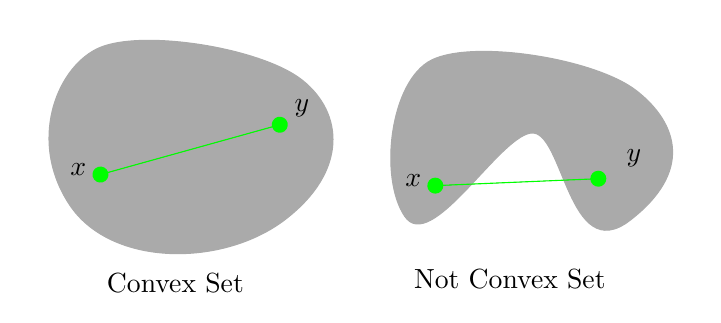
\begin{tikzpicture}[x=0.75pt,y=0.75pt,yscale=-1,xscale=1]
        %uncomment if require: \path (0,300); %set diagram left start at 0, and has height of 300
        
        %Shape: Polygon Curved [id:ds2968865898515556] 
        \draw  [color={rgb, 255:red, 170; green, 170; blue, 170 }  ,draw opacity=1 ][fill={rgb, 255:red, 170; green, 170; blue, 170 }  ,fill opacity=1 ] (153,42.83) .. controls (173,32.83) and (232,42) .. (252,57.83) .. controls (272,73.67) and (274,101.67) .. (244,124.83) .. controls (214,148) and (160,148) .. (140,118) .. controls (120,88) and (133,52.83) .. (153,42.83) -- cycle ;
        %Straight Lines [id:da27627405204315614] 
        \draw [color={rgb, 255:red, 0; green, 255; blue, 0 }  ,draw opacity=1 ][fill={rgb, 255:red, 0; green, 0; blue, 0 }  ,fill opacity=1 ]   (154.8,103.33) -- (241.2,79.33) ;
        \draw [shift={(241.2,79.33)}, rotate = 344.48] [color={rgb, 255:red, 0; green, 255; blue, 0 }  ,draw opacity=1 ][fill={rgb, 255:red, 0; green, 255; blue, 0 }  ,fill opacity=1 ][line width=0.75]      (0, 0) circle [x radius= 3.35, y radius= 3.35]   ;
        \draw [shift={(154.8,103.33)}, rotate = 344.48] [color={rgb, 255:red, 0; green, 255; blue, 0 }  ,draw opacity=1 ][fill={rgb, 255:red, 0; green, 255; blue, 0 }  ,fill opacity=1 ][line width=0.75]      (0, 0) circle [x radius= 3.35, y radius= 3.35]   ;
        %Shape: Polygon Curved [id:ds906687188537532] 
        \draw  [color={rgb, 255:red, 170; green, 170; blue, 170 }  ,draw opacity=1 ][fill={rgb, 255:red, 170; green, 170; blue, 170 }  ,fill opacity=1 ] (314.33,48.17) .. controls (334.33,38.17) and (393.33,47.33) .. (413.33,63.17) .. controls (433.33,79) and (440,102.17) .. (410,125.33) .. controls (380,148.5) and (377.84,80.69) .. (362,83.33) .. controls (346.16,85.97) and (313.8,142.03) .. (301.33,123.33) .. controls (288.87,104.64) and (294.33,58.17) .. (314.33,48.17) -- cycle ;
        %Straight Lines [id:da8771843126448762] 
        \draw [color={rgb, 255:red, 0; green, 255; blue, 0 }  ,draw opacity=1 ][fill={rgb, 255:red, 0; green, 0; blue, 0 }  ,fill opacity=1 ]   (316.13,108.67) -- (394.67,105.33) ;
        \draw [shift={(394.67,105.33)}, rotate = 357.57] [color={rgb, 255:red, 0; green, 255; blue, 0 }  ,draw opacity=1 ][fill={rgb, 255:red, 0; green, 255; blue, 0 }  ,fill opacity=1 ][line width=0.75]      (0, 0) circle [x radius= 3.35, y radius= 3.35]   ;
        \draw [shift={(316.13,108.67)}, rotate = 357.57] [color={rgb, 255:red, 0; green, 255; blue, 0 }  ,draw opacity=1 ][fill={rgb, 255:red, 0; green, 255; blue, 0 }  ,fill opacity=1 ][line width=0.75]      (0, 0) circle [x radius= 3.35, y radius= 3.35]   ;
        
        % Text Node
        \draw (139.07,96.73) node [anchor=north west][inner sep=0.75pt]    {$x$};
        % Text Node
        \draw (247.07,66.13) node [anchor=north west][inner sep=0.75pt]  [color={rgb, 255:red, 0; green, 0; blue, 0 }  ,opacity=1 ]  {$y$};
        % Text Node
        \draw (300.4,102.07) node [anchor=north west][inner sep=0.75pt]    {$x$};
        % Text Node
        \draw (407.07,90.13) node [anchor=north west][inner sep=0.75pt]  [color={rgb, 255:red, 0; green, 0; blue, 0 }  ,opacity=1 ]  {$y$};
        % Text Node
        \draw (156.67,150) node [anchor=north west][inner sep=0.75pt]   [align=left] {Convex Set};
        % Text Node
        \draw (304.67,148) node [anchor=north west][inner sep=0.75pt]   [align=left] {Not Convex Set};
        \end{tikzpicture}
    \end{center}
\end{definition}
\begin{lemma}[]
    A ball in a normed Space is Convex
\end{lemma}
\begin{proof}[Proof]
    Let $x,y$ be two points in a ball $B(a,r) \implies ||x-a|| \leq r , ||y-a||<r$
    \\
    Now let 
    \begin{align*}
        z &= \alpha x + (1-\alpha)y \quad,\quad 0 \leq \alpha \leq 1
        \\
        z-a &= \alpha x + (1-\alpha)y-a
        \\
        &= \alpha x -\alpha a  + (1-\alpha)y-a + \alpha a 
        \\
        &= \alpha (x-a) + (1-\alpha)y-(1-\alpha)a
        \\
        &= \alpha (x-a) + (1-\alpha)(y-a)
        \\
        &\leq \alpha r + (1-\alpha)r
        \\
        &\leq r
    \end{align*}
    Thus $z \in B(a,r)$
    \[
        \therefore \left\{ z \in X : z = \alpha x + (1-\alpha)y \quad,\quad 0 \leq \alpha \leq 1 \right\} \subset B(a,r) \implies \text{$B(a,r)$ is Convex}
    \]
\end{proof}
\begin{definition}[Fixed Point]
    The fixed point of a mapping of a set $X$ into itself $T:X \to X$
    is an element $x \in X$, which is mapped by $T$ onto itself, that is $Tx=x$.
    
    Examples let $ T:\mathbb{R} \to \mathbb{R}$
    \begin{itemize}
        \item Consider the mapping $Tx = x^2$ it's fixed points are $\left\{ 0,1 \right\}$
        \item Consider the mapping $Tx = x$ it's fixed points are the whole $\mathbb{R}$ 
        \item Consider the mapping $Tx = x+1$ it has no fixed point
    \end{itemize}
\end{definition}
\begin{theorem}[Schauder Fixed Point Theorem]
    $ $ \newline
    Let $Q$ be a Convex and Closed subset of a Banach space then a continuous
    and Compact Operator
    \[
        T:Q \to Q
    \]
    Has at least one fixed point 
\end{theorem}

Now we have all the properties and definitions that we need now consider the following existence Theorem
\newpage
\begin{theorem}[Peano's Existence Theorem]
    $ $ \newline
    Let $0 \leq m-1 < \alpha < m $ and let $y(0),y^{(1)}(0),\dots,y^{(m-1)}(0) \in \mathbb{R}^d $ , $\eta>0,K>0$ 
    \\
    Consider the domain $\displaystyle D := \left\{ (t,y) : t \in [0, \eta] \quad,\quad \left|\left| y-\sum_{k=0}^{m-1} \frac{t^k}{k!} y^{(k)}(0) \right|\right| \leq K  \right\} $
    \\
    And that $f := D \to \mathbb{R}^d$ is continuous and bounded, with $M := \sup\limits_{(t,y)\in D} |f(t,y)|$. Moreover , let
    \begin{equation}
        \Omega := \begin{cases}
            \eta     & \text{\textit{if M=0}}
            \\
            \displaystyle \min\left\{\eta , \left(\frac{K\Gamma(\alpha+1)}{M}\right)^{\frac{1}{\alpha}} \right\} &\text{else}
        \end{cases}
    \end{equation}
    Then there exists a function $y(t) \in C[0, \Omega]$ solves the nonlinear Volterra integral equation (6.3).
\end{theorem}
\begin{proof}[Proof]
    Let 
    \begin{align}
        \notag y(t) &= \sum_{k=0}^{m-1} \frac{t^k}{k!} y^{(k)}(0) + \frac{1}{\Gamma(\alpha)}\int_{0}^{t} (t-s)^{\alpha-1}f(s,y(s)) \hquad ds
        \\
        &= g(t) + I^\alpha f(t,y(t))
    \end{align}
    And let the set 
    \[
        U := \left\{ y \in C[0, \eta] \quad,\quad ||y-g|| \leq K \right\}
    \]
    $U$ is a closed since the less than or "equal" condition and convex since it is a ball centered at $g$ subset of the Banach space of all continuous functions on $[0, \eta]$ Hence, $U$ is a Banach space too
    Since the polynomial $g(t)$ is an element of $U$, we also see that $U$ is not empty. 
    
    On this set $U$ we define the operator $T$ by
    \[
        Ty = g(t) + I^\alpha f(t,y(t))
    \]
    Using this operator, the equation (6.5) whose solvability we need to prove can be rewritten as
    \[
        Ty = y
    \]
    And thus, in order to prove our desired existence result, we have to show that $T$ has
    a fixed point. 
    
    We therefore proceed by investigating the properties of the operator $T$ more closely.
    
    Our first goal in this context is to show that $Ty \in U$ for $y \in U$. 
    \\
    It's clear that $Ty$ is Continuous
    \begin{align*}
        Ty &= g(t) + I^\alpha f(t,y(t)) 
        \\
        &= polynomial + I^\alpha (Continuous) 
        \\
        &= polynomial + Continuous = Continuous
    \end{align*}
    And for $Ty$ to be element in $U$ 
    \begin{align*}
        |Ty - g| &= \frac{1}{\Gamma(\alpha)} \left|\int_{0}^{t} (t-s)^{\alpha-1}f(s,y(s)) \hquad ds\right|
        \\
        &\leq \frac{1}{\Gamma(\alpha)} \int_{0}^{t} \left|(t-s)^{\alpha-1}\right|\left|f(s,y(s))\right| \hquad ds
        \\
        &\leq \frac{M}{\Gamma(\alpha)} \int_{0}^{t} (t-s)^{\alpha-1}\hquad ds
        \\
        &\leq \frac{M}{\Gamma(\alpha)} \frac{t^\alpha}{\alpha} = \frac{M t^\alpha}{\Gamma(\alpha+1)}
    \end{align*}
    We want this to be less than $K$ therefore 
    \begin{align*}
        \frac{M t^\alpha}{\Gamma(\alpha+1)} &\leq K
        \\
        t &\leq \left(\frac{K\Gamma(\alpha+1)}{M}\right)^{\frac{1}{\alpha}}
    \end{align*}
    Therefore $t$ must not grow more than $\displaystyle \left(\frac{K\Gamma(\alpha+1)}{M}\right)^{\frac{1}{\alpha}}$ and in the same time 
    $t$ is limited by $\eta$ therefore we can put the condition
    \[
        t \in [0 , \Omega] \quad,\quad \Omega = \min\left\{\eta , \left(\frac{K\Gamma(\alpha+1)}{M}\right)^{\frac{1}{\alpha}} \right\}
    \]
    Thus, we have shown that $Ty \in U$ if $y \in U[0,\Omega]$ i.e $T$ maps the set $U$ to itself.

    Since we want to apply Schauder's Fixed Point Theorem, all that
    remains now is to show that $T(U) := \{Ty : y \in U\}$ is a relatively compact set. This
    can be done by means of the Arzela Ascoli Theorem . For $y \in U$ we find that, for all $t \in [0,\Omega]$
    \begin{align*}
        |Ty| &= \left|g(t) + \frac{1}{\Gamma(\alpha)}\int_{0}^{t} (t-s)^{\alpha-1}f(s,y(s)) \hquad ds\right|
        \\
        &\leq ||g(t)||_{\infty} + \frac{1}{\Gamma(\alpha)}\int_{0}^{t} (t-s)^{\alpha-1}|f(s,y(s))| \hquad ds
        \\
        &\leq ||g(t)||_{\infty} + \frac{M}{\Gamma(\alpha)}\frac{t^\alpha}{\alpha}
        \\
        &\leq ||g(t)||_{\infty} + \frac{M\Omega^\alpha}{\Gamma(\alpha+1)}
        \\
        &\leq ||g(t)||_{\infty} + K
    \end{align*}
    \begin{enrichment*}{Chebyshev Norm}
        the supremum norm, the Chebyshev norm, the infinity norm on a set S is defined as
        \[
            ||f(t)||_{\infty} = \sup\limits_{t\in S} |f(t)|
        \]
    \end{enrichment*}
    Which is the required boundedness property. 
    
    Moreover, the equicontinuity property let $0 \leq t_1 \leq t_2 \leq \Omega$
    \begin{align*}
        |Ty(t_2)-Ty(t_1)| &= |g(t_2)-g(t_1) + I^\alpha f(t_2,y(t_2))-I^\alpha f(t_1,y(t_1))|
        \\
        &\leq |g(t_2)-g(t_1)| + I^\alpha \left| f(t_2,y(t_2))-f(t_1,y(t_1)) \right|
        \intertext{Thus if $|t_2-t_1| < \delta $}
        &\leq \epsilon_1 + I^\alpha \epsilon_2
        \\
        &\leq \epsilon_1 + \epsilon_2 \frac{t^\alpha}{\Gamma(\alpha+1)}
        \\
        &\leq \epsilon_1 + \epsilon_2 \frac{\Omega^\alpha}{\Gamma(\alpha+1)}
        \\
        &\leq \epsilon_1 + \epsilon_2 \frac{K}{M} < \epsilon
    \end{align*}
    Therefore the set $T(U)$ is equicontinuous. 
    \\
    Thus Arzela Ascoli Theorem yields that $T(U)$ is relatively compact, and hence Schauder's Fixed Point Theorem asserts that $T$ has a fixed point.
    % If $M = 0$ then $f(t,y) = 0$ for all $(t,y) \in [0,\eta]\times U$. 
    % \\
    % In this case it is evident that the function $y:[0,\eta] \to \mathbb{R}$ with 
    % \[
    %     y(t) = g(t) = \sum_{k=0}^{m-1} \frac{t^k}{k!} y^{(k)}(0)
    % \]
    % Is a solution of the initial value problem.
\end{proof}
We reached to that there exists a Continuous solution $y(t)$ that solves the Volterra integral equation (6.3)
to make it solve the IVP (6.2) we must prove the equivalence between them 
\[
    y(t) = g(t) + I^{\alpha}f(t,y(t))
\]
Applying Caputo Derivative for both sides we get 
\begin{align*}
    \leftindex[I]^C {D^{\alpha}} y(t) &= \leftindex[I]^C {D^{\alpha}} g(t) + \leftindex[I]^C {D^{\alpha}} I^{\alpha}f(t,y(t))
    \\
    &= \leftindex[I]^C {D^{\alpha}} I^{\alpha}f(t,y(t))
    \\
    &= I^{m-\alpha} \dv[m]{}{t} I^{\alpha}f(t,y(t))
    \\
    &= I^{m-\alpha} \dv[m]{}{t} I^{\alpha+m-m}f(t,y(t))
    \\
    &= I^{m-\alpha} D^{m-\alpha}f(t,y(t)) = f(t,y(t))
\end{align*}
A condition must be taking into account that the right hand side must be Caputo differentiable thus 
we must put the condition that $I^{\alpha}f(t,y(t)) \in AC^{m}[0,\Omega]$ and this yields that 
\begin{align*}
    y(t) = g(t) + I^{\alpha}f(t,y(t)) = polynomial + AC^{m} \in AC^{m}
\end{align*}
This condition remove the counter Example that have been used in [10] that is by taking 
\[
    f(t,y(t)) = D^\alpha \mathcal{W}(t)
\]
Where $\mathcal{W}(t)$ is Weierstrass function because $D^\alpha \mathcal{W}(t)$ is continuous
we can say that 
\begin{align*}
    y(t) &= g(t) + I^{\alpha}f(t,y(t))
    \\
    &= g(t) + I^{\alpha} D^\alpha \mathcal{W}(t)
    \\
    &= g(t) + \mathcal{W}(t)
\end{align*}
If we apply Caputo Derivative the Derivative of $\mathcal{W}(t)$ the expression will be "meaningless"

Thus $f(t,y(t))$ being continuous is not enough to get the equivalence of the IVP and Volterra IE%and other condition must be taken into account that is $I^{\alpha}f(t,y(t)) \in AC^{m}[0,\Omega]$


Schauder fixed point Theorem only guarantee the existence to get the uniqueness consider the following

The classical Picard-Lindelöf theorem can be generalized to the fractional setting
in the same way: If the given function $f$ is continuous and bounded and satisfies 
a Lipschitz condition with respect to the second variable, then uniqueness of the 
continuous solution to the integral equation (6.3) can be guaranteed.

\begin{theorem}[Picard-Lindelöf Uniqueness Theorem]
    Assume the hypotheses of Theorem (6.4). Moreover, let $f$ fulfill a Lipschitz condition with respect to the second variable,
    that is,
    \[
        \left|\left| f(t,y_1)-f(t,y_2) \right|\right| \leq L \left|\left| y_1-y_2 \right|\right|
    \]
    Where $L$ is Lipschitz constant Then there exists a uniquely defined function $y(t) \in C[0, \Omega]$ solves the integral equation (6.3)
\end{theorem}
To Proof the uniqueness we are going to use the successive approximation method
\[
        y_n(t) = g(t) + \frac{1}{\Gamma(\alpha)} \int_{0}^{t} (t-s)^{\alpha-1}f(s,y_{n-1}(s)) \hquad ds
\]
In the case $n = 0$ it is obvious.
\[
    y_0(t) = g(t)
\]
If $n = 1$, then we have:
\begin{align*}
    |y_1(t)-y_0(t)| &= \left| \frac{1}{\Gamma(\alpha)} \int_{0}^{t} (t-s)^{\alpha-1}f(s,y_{0}(s)) \hquad ds \right|
    \\
    &\leq \frac{1}{\Gamma(\alpha)} \int_{0}^{t} \left|(t-s)^{\alpha-1}\right|\left|f(s,y_{0}(s))\right| \hquad ds 
    \\
    &\leq \frac{M}{\Gamma(\alpha)} \int_{0}^{t} (t-s)^{\alpha-1} \hquad ds 
    \\
    &\leq \frac{M}{\Gamma(\alpha)}\frac{t^\alpha}{\alpha} \leq \frac{M\Omega^\alpha}{\Gamma(\alpha+1)} < K
    \\
    |y_2(t)-y_1(t)| &= \left| \frac{1}{\Gamma(\alpha)} \int_{0}^{t} (t-s)^{\alpha-1}\left[f(s,y_{1}(s))-f(s,y_{0}(s))\right] \hquad ds \right|
    \\
    &\leq \frac{L}{\Gamma(\alpha)} \int_{0}^{t} (t-s)^{\alpha-1} \left|y_1-y_0\right| \hquad ds 
    \\
    &\leq \frac{LK}{\Gamma(\alpha)} \int_{0}^{t} (t-s)^{\alpha-1} \hquad ds 
    \\
    &<  \frac{LK^2}{M}
    \\
    |y_3(t)-y_2(t)| &= \left| \frac{1}{\Gamma(\alpha)} \int_{0}^{t} (t-s)^{\alpha-1}\left[f(s,y_{2}(s))-f(s,y_{1}(s))\right] \hquad ds \right|
    \\
    &\leq \frac{L}{\Gamma(\alpha)} \int_{0}^{t} (t-s)^{\alpha-1} \left|y_2-y_1\right| \hquad ds 
    \\
    &\leq \frac{L^2K^2}{M\Gamma(\alpha)} \int_{0}^{t} (t-s)^{\alpha-1} \hquad ds 
    \\
    &< \frac{L^2K^3}{M^2}
\end{align*}
And so on we get 
\[
    |y_{n+1}(t)-y_{n}(t)| \leq K \left(\frac{LK}{M}\right)^{n}
\]
Now summing over $n$ to get the solutions
\[
    y_{0}(t) + \sum_{k=0}^{n} y_{k+1}(t)-y_{k}(t) = y_{0}(t) + y_{n+1}(t)-y_{n}(t)+y_{n}(t)-\dots-y_{0}(t) = y_{n+1}(t)
\]
Take the limit as $n \to \infty$ we get 
\begin{align*}
    \lim_{n \to \infty} y_{n+1}(t) &= y_{0}(t) + \lim_{n \to \infty} \sum_{k=0}^{n} y_{k+1}(t)-y_{k}(t)
    \\
    y(t) &= y_{0}(t) + \sum_{k=0}^{\infty} y_{k+1}(t)-y_{k}(t)
\end{align*}
Using Weierstrass Test 
\[
    \sum_{k=0}^{\infty} |y_{k+1}(t)-y_{k}(t)| \leq \eta \sum_{k=0}^{\infty} \left(\frac{LK}{M}\right)^{k}
\]
The series is convergent if $\displaystyle \frac{LK}{M} < 1$

Thus the sequence $\{y_n(t)\}$ is uniform convergent to a function $y(t)$ for $t \in [0, \Omega]$.
\begin{enrichment*}{The Weierstrass Test}
    Suppose that $\{f_n(t)\}$ is a sequence of real functions defined on a set $A$, 
    and there is a sequence of positive numbers $\{R_n\}$ satisfying:
    \[
        \forall n > 0 , \forall t \in A \quad,\quad |f_n(t)|<R_n \quad,\quad \sum_{n=0}^{\infty} R_n < \infty
    \]
    Then the series
    \[
        \sum_{n=0}^{\infty} f_n(t)
    \]
    Is convergent
\end{enrichment*}
\begin{proof}[Proof Theorem (6.5)]
    Let there is two solutions $y_1 , y_2$ satisfy the equation
    \[
        y(t) = g(t) + I^{\alpha}f(t,y(t))
    \]
    Therefore
    \begin{align*}
        y_1(t) - y_2(t) &= g(t) - g(t) + I^{\alpha}f(t,y_1(t)) - I^{\alpha}f(t,y_2(t))
        \\
        ||y_1(t) - y_2(t)|| &\leq I^{\alpha}||f(t,y_1(t)) - f(t,y_2(t))||
        \\
        &\leq L I^{\alpha}||y_1(t) - y_2(t)||
        \\
        &\leq ||y_1(t) - y_2(t)|| L \frac{t^\alpha}{\Gamma(\alpha+1)}
        \\
        &\leq ||y_1(t) - y_2(t)|| \frac{LK}{M}
        \\
        ||y_1(t) - y_2(t)|| (1-\frac{LK}{M}) &\leq 0
        \intertext{Because $\displaystyle \frac{LK}{M} < 1$}
        ||y_1(t) - y_2(t)|| &\leq 0
        \\
        ||y_1(t) - y_2(t)|| &= 0
        \\
        y_1(t) &= y_2(t) 
    \end{align*}
\end{proof}
\newpage
\subsubsection{Stability}
In many important situations, the solutions to the differential equation exist on
the unbounded interval $[0,\infty)$. In such a case, it is often required to investigate the behavior of
solutions as $t \to \infty$

The Solutions of a problem are called Stable if they depends on the given data in a continuous way

In integer differential equation the given data was only referring to the initial conditions 

Consider
\[
    \frac{dy(t)}{dt} = f(t,y(t)) \dquad t>0
\]
Let $y(t),y^*(t)$ be solutions to the equation with different initial values $y(0)=a , y^*(0)=b$

We say that the solutions of equation are \textbf{stable} if and only if
\[
    \forall \epsilon >0 \  , \ \exists \delta >0 \text{  s.t  } |a-b| < \delta \implies |y(t) - y^*(t)| \leq \epsilon
\]
Moreover we say that the solutions of equation are \textbf{asymptotically stable} if and only if they
satisfies the previous Conditions and $\displaystyle \lim_{t \to \infty} (y(t) - y^*(t)) = 0$

Furthermore we say that the solutions of equation are \textbf{unstable}
if there exists a unique initial value such that the solution of the differential 
equation subject to that initial condition is bounded and the solutions to the 
differential equation subject to other initial values are unbounded


One important difference between the fractional and the classical setting is the meaning of the expression “the given data”.

In the classical theory, we usually assumes that the initial values and the function $f$ to be given
and then the behavior of the solution under perturbations of these expressions is discussed. 

In the fractional setting, however, it is additionally possible to perturb the order $\alpha$ of 
the differential equation, and so this new feature must be taken into account as well. 

\subsubsection*{Well-Posedness}
A problem is called well-posed if it has the following three properties:
\begin{enumerate}
    \item A solution exists
    \item The solution is unique
    \item The solution depends on the given data in a continuous way (stable)
\end{enumerate}

\subsubsection{Separation Of Solutions}
Another result from the theory of first order differential equations states that
the graphs of two solutions of the same differential equation that satisfy different initial
conditions can never meet or cross each other if the given function $f$ satisfies a Lipschitz
condition. This statement is indeed valid only for first-order problems, that is,
for problems with exactly one initial condition. Thus a similar result for FDE can only be shown 
for IVPs with exactly one initial condition, that is, for problems with an order $\alpha \in (0, 1)$

It can be explained by the visualization indicated in Figure 1.
\begin{figure*}[h]
    \begin{minipage}[l]{.5\textwidth}
      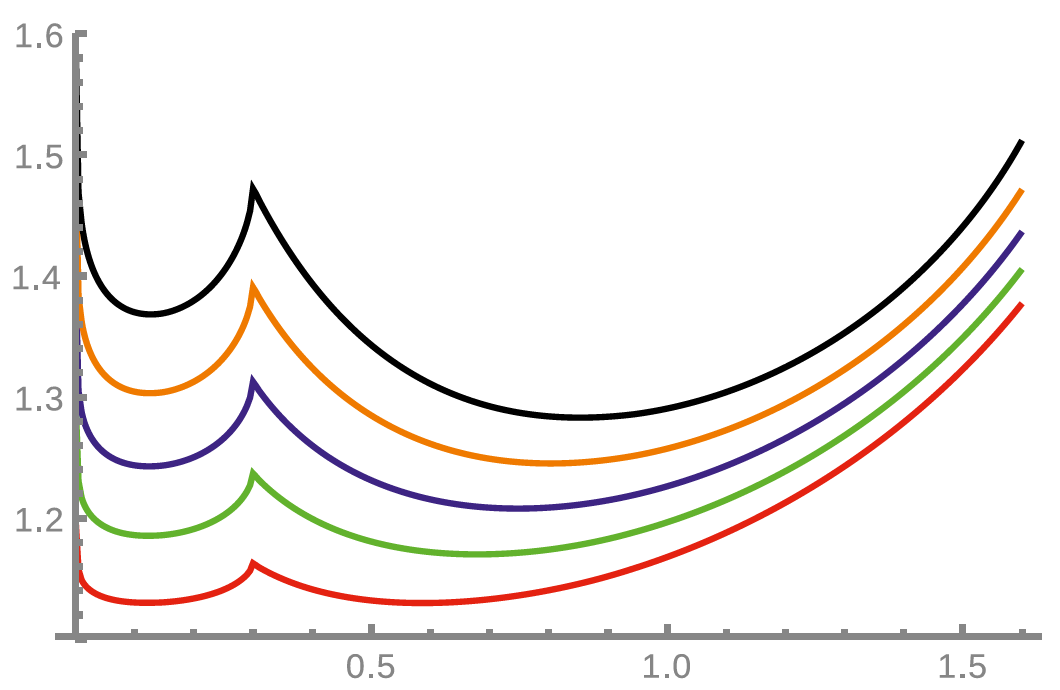
\includegraphics[scale = .25]{plot/3.png}
    \end{minipage}  
    \begin{minipage}[r]{.5\textwidth}
      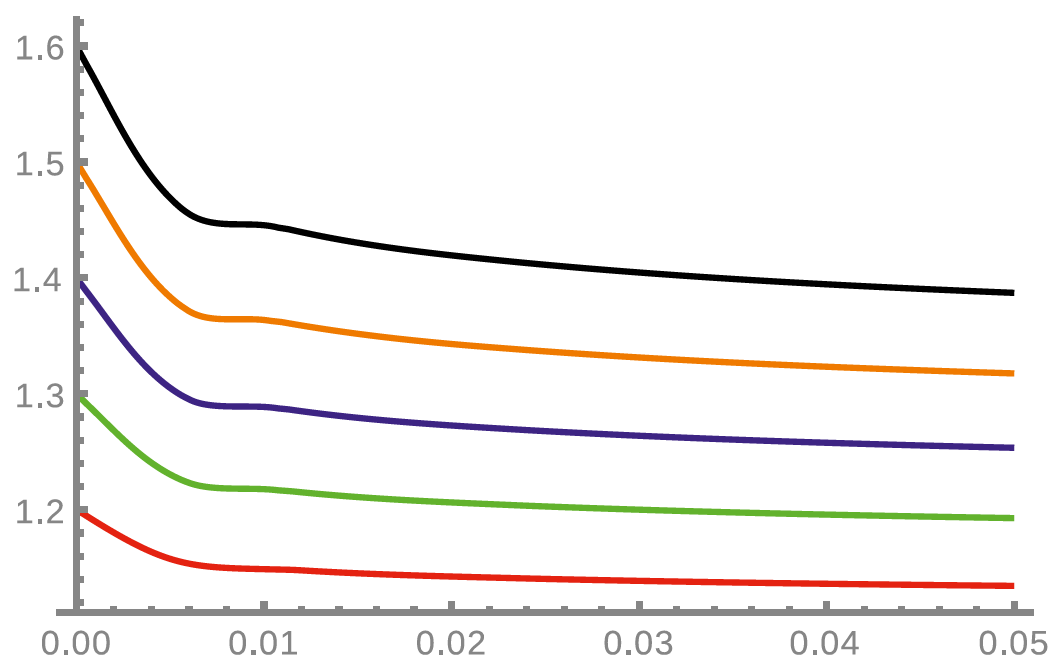
\includegraphics[scale = .25]{plot/4.png}
    \end{minipage} 
    \caption{
        Graphs of solutions to the differential equation $\leftindex[I]^C {D^{0.28}}y(t) = \sqrt{|0.3-t|} \sin(3y(t))+ 0.3t^3$
        with initial conditions $y(0) = 1.2$ (red), $y(0) = 1.3$ (green), $y(0) = 1.4$ (blue), $y(0) = 1.5$ (orange)
        and $y(0) = 1.6$ (black), plotted over the interval $[0, 1.6]$ (left) and zoom of this picture to the interval
        $[0, 0.05]$ (right). It can be observed that the graphs never meet or cross each other.
    } 
\end{figure*}

\newpage
\subsection{Linear Fractional Differential Equations (LFDE)}
A linear FDE is an equation of form
\[
    \left(\leftindex[I]^C {D^{\alpha_m}} + a_{m-1}(t)\leftindex[I]^C {D^{\alpha_{m-1}}} + \dots + a_{1}(t)\leftindex[I]^C {D^{\alpha_{1}}} + a_{1}(t) \right) y(t) = f(t)
\]
With the conditions:
\[
    y^{(k)}(0) = \beta_k \quad,\quad k = 0,1,2,\dots,m-1
\]
\begin{theorem}[Existence And Uniqueness Of LFDE]
    If $f(t)$ is bounded on $(0, T)$ and $a_{k}(t)$ , $k = {0, 1, \dots , m-1}$ 
    are continuous functions on $[0, T]$, the equation has a unique solution.
\end{theorem}
In the particular case where the given differential equation is linear, it is often possible
to write up the solutions in closed form.
\begin{example}
    Show that 
    \[
        y(t) = \frac{1}{\Gamma(\alpha)}\int_{0}^{t} (t-s)^{\alpha-1}f(s) \hquad ds
    \]
    Solves the IVP 
    \[
        \begin{cases}
            \leftindex[I]^C {D^{\alpha}} y(t) = f(t)    \quad&,\quad m-1<\alpha<m
            \\
            I.C \Longrightarrow y^{(k)}(0) = 0 \quad&,\quad k = 0,1,2,\dots,m-1
        \end{cases}
    \]
    \textit{ \textbf{Sol.} } We apply the Laplace transform
        \begin{align*}
            \mathcal{L}\left[\leftindex[I]^C {D^{\alpha}} y(t)\right] &= \mathcal{L}[f(t)]
            \\
            s^{\alpha} Y(s) &= F(s)
            \\
            Y(s) &= s^{-\alpha}F(s)
            \\
            \mathcal{L}[y(t)] &= \mathcal{L}\left[I^{\alpha}f(t)\right]
            \\
            y(t) &= I^{\alpha}f(t) = \frac{1}{\Gamma(\alpha)}\int_{0}^{t} (t-s)^{\alpha-1}f(s) \hquad ds
        \end{align*}
\end{example}
\begin{enrichment*}{Laplace of Mittag Leffler Function }
    \[
        \mathcal{L}\left[t^{\beta-1} E_{\alpha,\beta}(\lambda t^\alpha)\right] = \frac{s^{\alpha - \beta}}{s^{\alpha}-\lambda}
    \]
\end{enrichment*}
\begin{example}
    Show that 
    \[
        y(t) = \sum_{k=0}^{m-1} \beta_k t^{k} E_{\alpha,k+1}(\lambda t^\alpha)
    \]
    Solves the IVP 
    \[
        \begin{cases}
            \leftindex[I]^C {D^{\alpha}} y(t) = \lambda y(t)    \quad&,\quad m-1<\alpha<m
            \\
            I.C \Longrightarrow y^{(k)}(0) = \beta_k \quad&,\quad k = 0,1,2,\dots,m-1
        \end{cases}
    \]
    \textit{ \textbf{Sol.} } We apply the Laplace transform
        \begin{align*}
            \mathcal{L}\left[\leftindex[I]^C {D^{\alpha}} y(t)\right] &= \lambda \mathcal{L}[y(t)]
            \\
            s^{\alpha} Y(s) - \sum_{k=0}^{m-1} s^{\alpha-k-1} y^{(k)}(0) &= \lambda Y(s)
            \\
            Y(s) &= \sum_{k=0}^{m-1} \frac{s^{\alpha-k-1}}{s^{\alpha}-\lambda} \beta_k
            \\
            \mathcal{L}[y(t)] &= \sum_{k=0}^{m-1} \mathcal{L}\left[\beta_k t^{k} E_{\alpha,k+1}(\lambda t^\alpha)\right]
            \\
            \mathcal{L}[y(t)] &= \mathcal{L}\left[\sum_{k=0}^{m-1} \beta_k t^{k} E_{\alpha,k+1}(\lambda t^\alpha)\right]
            \\
            y(t) &= \sum_{k=0}^{m-1} \beta_k t^{k} E_{\alpha,k+1}(\lambda t^\alpha)
        \end{align*}
\end{example}
In example (6.1.4) if we take special case when $m-1 = 0$ and for $\lambda = -1$. 
\[
    y(t) = \beta_0 E_{\alpha,1}(-t^\alpha)
\]
The cases $\alpha = 1$ and $\alpha = 2$
reduce to the well known statements that are the exponential function $E_{1,1}(-t) = e^{-t}$ and
the cosine $E_{2,1}(-t^2) = cos(t)$ solve the given first and second order IVPs.

This observation indicates that the solutions to the general problem of order $\alpha$ 
decay in a monotonic way for $\alpha = 1$ and exhibit persistent oscillations for $\alpha = 2$ if $\lambda$ is
a negative real number. 
And the behavior of the solution in the cases $1 < \alpha < 2$ and $0 < \alpha < 1$. 
The associated results are illustrated in Figure 2
\begin{figure*}[h]
    \begin{minipage}[l]{.5\textwidth}
      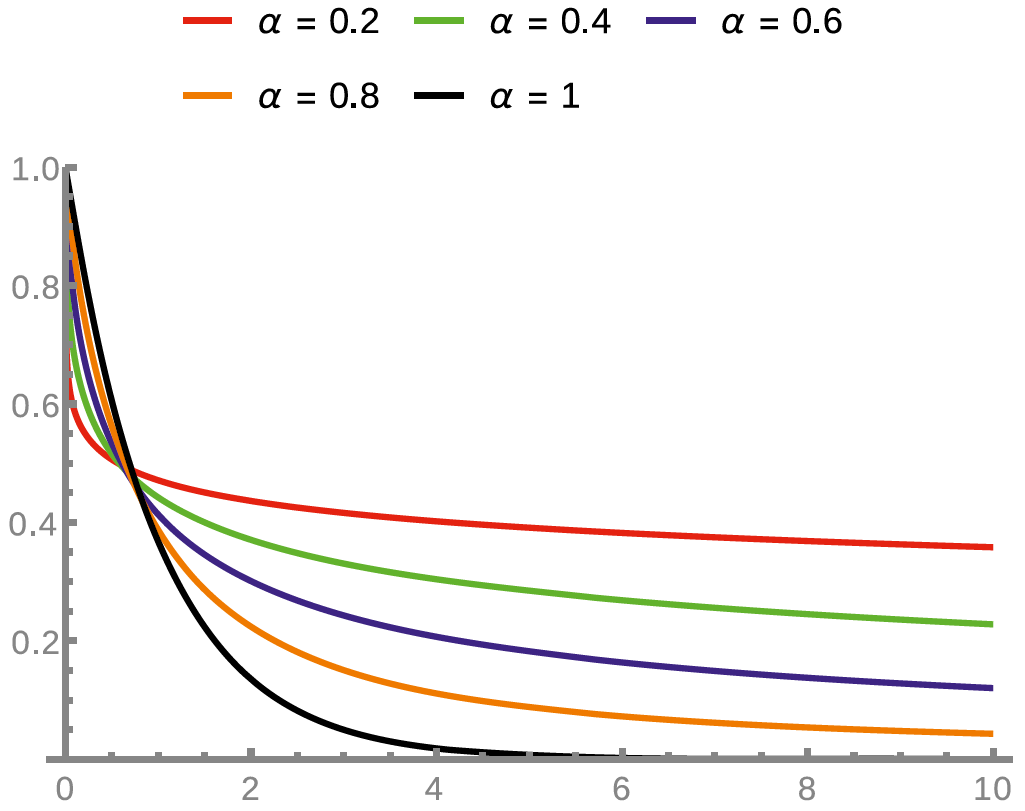
\includegraphics[scale = .25]{plot/1.png}
    \end{minipage}  
    \begin{minipage}[r]{.5\textwidth}
      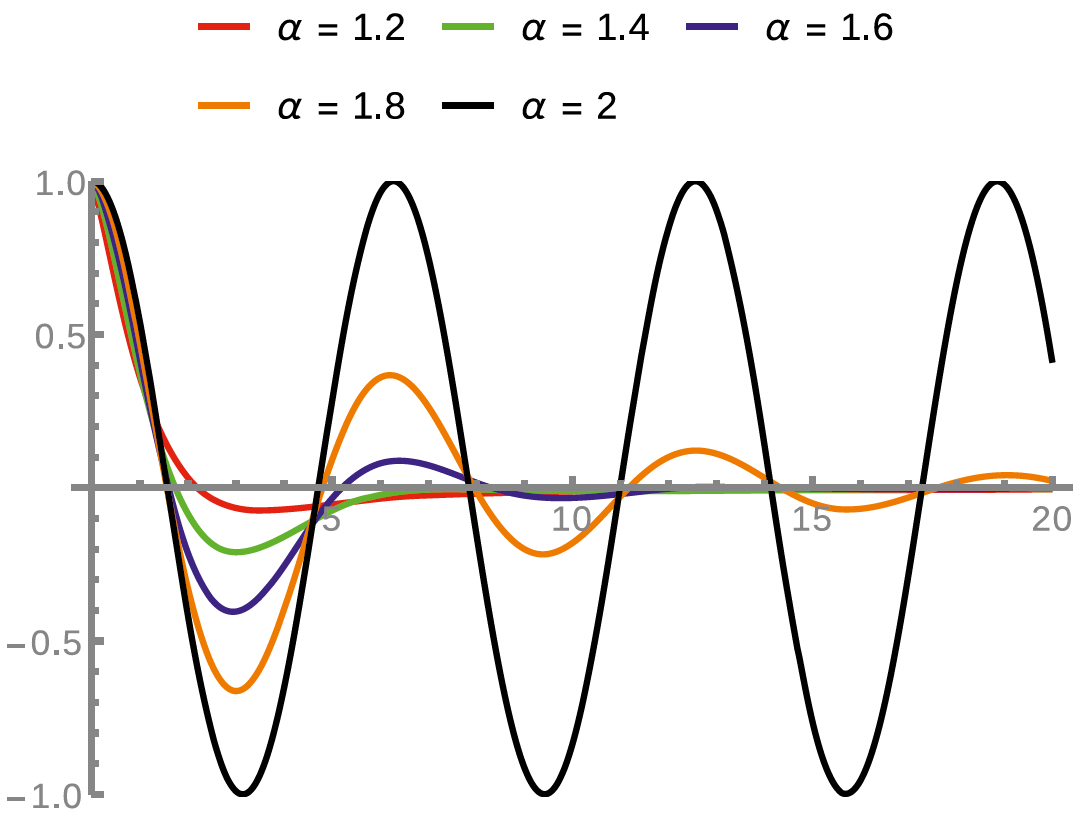
\includegraphics[scale = .25]{plot/2.png}
    \end{minipage} 
    \caption{Plots of $y(t) = E_{\alpha}(-t^\alpha)$ for various $\alpha \in (0, 1]$ (left) and $\alpha \in (1, 2]$ (right).} 
\end{figure*}

\begin{example}
    Show that 
    \[
        y(t) = \beta + t^{\alpha} \sum_{n=0}^{\infty} \frac{f^{(n)}(0)}{\Gamma(n+\alpha+1)}t^n
    \]
    Solves the IVP 
    \[
        \begin{cases}
            \leftindex[I]^C {D^{\alpha}} y(t) = f(t)    \quad,\quad 0<\alpha<1
            \\
            I.C \Longrightarrow y(0) = \beta
        \end{cases}
    \]
    \textit{ \textbf{Sol.} } We expand $f(t)$ using Taylor expansion and apply the Laplace transform
        \begin{align*}
            \mathcal{L}[\leftindex[I]^C {D^{\alpha}} y(t)] &= \mathcal{L}[f(t)]
            \\
            s^{\alpha} Y(s) - \beta s^{\alpha-1} &= \mathcal{L}\left[\sum_{n=0}^{\infty} \frac{f^{(n)}(0)}{\Gamma(n+1)}t^n\right]
            \\
            Y(s) &= \frac{\beta}{s} + \sum_{n=0}^{\infty} \frac{f^{(n)}(0)}{\Gamma(n+1)}\frac{1}{s^{\alpha}}\mathcal{L}[t^n]
            \\
            \mathcal{L}[y(t)] &= \mathcal{L}[\beta] + \sum_{n=0}^{\infty} \frac{f^{(n)}(0)}{\Gamma(n+1)}\frac{1}{s^{\alpha}}\frac{\Gamma(n+1)}{s^{n+1}}
            \\
            \mathcal{L}[y(t)] &= \mathcal{L}[\beta] + \sum_{n=0}^{\infty} f^{(n)}(0) \frac{1}{s^{n+\alpha+1}}
            \\
            \mathcal{L}[y(t)] &= \mathcal{L}[\beta] + \sum_{n=0}^{\infty} f^{(n)}(0) \mathcal{L}\left[\frac{t^{n+\alpha}}{\Gamma(n+\alpha+1)}\right]
            \\
            y(t) &= \beta + t^{\alpha} \sum_{n=0}^{\infty} \frac{f^{(n)}(0)}{\Gamma(n+\alpha+1)}t^n
        \end{align*}
\end{example}
% \newpage
\begin{example}
    Solve the in-homogeneous IVP 
    \[
        \begin{cases}
            \leftindex[I]^C {D^{\alpha}} y(t) = \lambda y(t) + Q(t)   \quad&,\quad m-1<\alpha<m
            \\
            I.C \Longrightarrow y^{(k)}(0) = \beta_k \quad&,\quad k = 0,1,2,\dots,m-1
        \end{cases}
    \]
    Where $Q \in C[0, h]$ is a given function 

    \textit{ \textbf{Sol.} } As we did previously we expand $Q(t)$ using Taylor expansion and apply the Laplace transform
    \begin{align*}
        \mathcal{L}\left[\leftindex[I]^C {D^{\alpha}} y(t)\right] &= \lambda \mathcal{L}[y(t)] + \mathcal{L}\left[\sum_{n=0}^{\infty} \frac{Q^{(n)}(0)}{\Gamma(n+1)}t^n\right]
        \\
        s^{\alpha} Y(s) - \sum_{k=0}^{m-1} s^{\alpha-k-1} y^{(k)}(0) &= \lambda Y(s) + \sum_{n=0}^{\infty} Q^{(n)}(0) s^{-n-1} 
        \\
        Y(s) &= \sum_{k=0}^{m-1} \frac{s^{\alpha-k-1}}{s^{\alpha}-\lambda} \beta_k + \sum_{n=0}^{\infty} Q^{(n)}(0) \frac{s^{-n-1} }{s^{\alpha}-\lambda}
        \\
        \mathcal{L}[y(t)] &= \sum_{k=0}^{m-1} \mathcal{L}\left[\beta_k t^{k} E_{\alpha,k+1}(\lambda t^\alpha)\right] + \sum_{n=0}^{\infty} Q^{(n)}(0) \frac{s^{\alpha-\alpha-n-1} }{s^{\alpha}-\lambda}
        \\
        \mathcal{L}[y(t)] &= \mathcal{L}\left[\sum_{k=0}^{m-1} \beta_k t^{k} E_{\alpha,k+1}(\lambda t^\alpha)\right] + \sum_{n=0}^{\infty} \mathcal{L}\left[Q^{(n)}(0) t^{\alpha+n} E_{\alpha,\alpha+n+1}(\lambda t^\alpha)\right]
        \\
        \mathcal{L}[y(t)] &= \mathcal{L}\left[\sum_{k=0}^{m-1} \beta_k t^{k} E_{\alpha,k+1}(\lambda t^\alpha)\right] + \mathcal{L}\left[\sum_{n=0}^{\infty} Q^{(n)}(0) t^{\alpha+n} E_{\alpha,\alpha+n+1}(\lambda t^\alpha)\right]
        \\
        \tag{6.7} y(t) &= \sum_{k=0}^{m-1} \beta_k t^{k} E_{\alpha,k+1}(\lambda t^\alpha) + \sum_{n=0}^{\infty} Q^{(n)}(0) t^{\alpha+n} E_{\alpha,\alpha+n+1}(\lambda t^\alpha)
        \intertext{Using Mittag Leffler function recursion relation $\displaystyle E_{\alpha,\alpha+\beta}(z) = \frac{1}{z}\left[E_{\alpha,\beta}(z) - \frac{1}{\Gamma(\beta)}\right]$}
        &= \sum_{k=0}^{m-1} \beta_k t^{k} E_{\alpha,k+1}(\lambda t^\alpha) + \sum_{n=0}^{\infty} Q^{(n)}(0) t^{\alpha+n} \frac{1}{\lambda t^\alpha}\left[E_{\alpha,n+1}(z) - \frac{1}{\Gamma(n+1)}\right]
        \\
        &= \sum_{k=0}^{m-1} \beta_k t^{k} E_{\alpha,k+1}(\lambda t^\alpha) + \frac{1}{\lambda}\sum_{n=0}^{\infty} Q^{(n)}(0) t^{n}E_{\alpha,n+1}(z) - \frac{Q(t)}{\lambda}
        \setcounter{equation}{7}
    \end{align*}
Another way using the superposition principle
\begin{enrichment*}{The Superposition Principle}
    The solution of the in-homogeneous equation can be written as the 
    sum of the solution of the homogeneous equation, and a particular 
    solution of the in-homogeneous equation.
\end{enrichment*}
We can break the problem into the following two problems
\[
    \begin{cases}
        \leftindex[I]^C {D^{\alpha}} y_h(t) = \lambda y_h(t)  \quad&,\quad m-1<\alpha<m
        \\
        I.C \Longrightarrow y_h^{(k)}(0) = \beta_k \quad&,\quad k = 0,1,2,\dots,m-1
    \end{cases}
\]
\[
    \begin{cases}
        \leftindex[I]^C {D^{\alpha}} y_p(t) = \lambda y_p(t) + Q(t)   \quad&,\quad m-1<\alpha<m
        \\
        I.C \Longrightarrow y_p^{(k)}(0) = 0 \quad&,\quad k = 0,1,2,\dots,m-1
    \end{cases}
\]
Where $y = y_h + y_p$ solves the original problem.
From example (6.3.2) we got that
\[
    y_h(t) = \sum_{k=0}^{m-1} \beta_k t^{k} E_{\alpha,k+1}(\lambda t^\alpha)
\]
Now for the second problem take Laplace Transform for it 
\begin{align*}
    \mathcal{L}\left[\leftindex[I]^C {D^{\alpha}} y_p(t)\right] &= \lambda \mathcal{L}[y_p(t)] + \mathcal{L}\left[\sum_{n=0}^{\infty} \frac{Q^{(n)}(0)}{\Gamma(n+1)}t^n\right]
    \\
    s^{\alpha} Y_p(s) &= \lambda Y_p(s) + \sum_{n=0}^{\infty} Q^{(n)}(0) s^{-n-1} 
    \\
    Y_p(s) &= \sum_{n=0}^{\infty} Q^{(n)}(0) \frac{s^{-n-1} }{s^{\alpha}-\lambda} = \sum_{n=0}^{\infty} Q^{(n)}(0) \frac{s^{\alpha-\alpha-n-1} }{s^{\alpha}-\lambda}
    \\
    \mathcal{L}[y_p(t)] &= \sum_{n=0}^{\infty} \mathcal{L}\left[Q^{(n)}(0) t^{\alpha+n} E_{\alpha,\alpha+n+1}(\lambda t^\alpha)\right]
    \\
    \mathcal{L}[y_p(t)] &= \mathcal{L}\left[\sum_{n=0}^{\infty} Q^{(n)}(0) t^{\alpha+n} E_{\alpha,\alpha+n+1}(\lambda t^\alpha)\right]
    \\
    y_p(t) &= \sum_{n=0}^{\infty} Q^{(n)}(0) t^{\alpha+n} E_{\alpha,\alpha+n+1}(\lambda t^\alpha)
\end{align*}
Adding $y_h + y_p$ we get the result (6.7)
\end{example}
\begin{enrichment*}{Duhamel's Principle}
    If one can solve an IVP for a homogeneous linear differential equation then an in-homogeneous linear differential equation can be solved as well.
\end{enrichment*} 
\newpage
\subsection{Nonlinear Equations}
Now we will discuss One of the methods to solve Nonlinear FDE which is The Adomian Decomposition Method

The Adomian method applied to the ordinary and partial differential equations of integer order was extended 
also to the case of FDE.
\subsubsection{The Adomian Decomposition Method (ADM)}
Before we talk about how to solve FDE using ADM let us first see how it work 

Consider the problem
\begin{equation}
    \begin{cases}
        \displaystyle \pdv{u(x,t)}{t} + L(u(x,t)) + N(u(x,y)) = g(x,t)
        \\
        I.C \Longrightarrow \displaystyle u(x,0) = \phi(x)
    \end{cases}
\end{equation}
This is nonlinear partial differential equation of integer order where $L(u(x,t))$ is the linear part and $N(u(x,t))$ is the non-linear part
We will discuss it's solution by ADM
\\
Now, Integrate (6.8) from $0 \to t$
\begin{equation}
    u(x,t) = \phi(x) - \int_{0}^{t} L(u(x,s)) \hquad ds  - \int_{0}^{t} N(u(x,s)) \hquad ds  + \int_{0}^{t} g(x,s) \hquad ds
\end{equation}
Set
\begin{equation}
    u(x,t) = \sum_{n=0}^{\infty} u_n(x,y)
\end{equation}
\begin{equation}
    N(u(x,t)) = \sum_{n=0}^{\infty} A_n(x,y)
\end{equation}
Where $A_0,A_1,A_2,\dots$ are \textbf{Adomian Polynomials} defined as:
\[
    A_n(x,y) = \frac{1}{n!} \dv[n]{}{\lambda} \left( N \left( \sum_{j=0}^{n}\lambda^j u_j \right) \right)
\]
Substitute equations (6.10),(6.11) into (6.9) we get
\begin{equation*}
    u(x,y) = \sum_{n=0}^{\infty}u_n(x,t) = \phi(x) + \int_0^t g(x,s) \hquad ds - \int_0^t L \left(\sum_{n=0}^{\infty}u_n(z,t)\right)  - \int_0^t \sum_{n=0}^{\infty}A_n(x,s) \hquad ds
\end{equation*}
Now,
\begin{align*}
    u_0 & = \phi(x) + \int_0^t g(x,s) \hquad ds                 \\
    u_1 & = -\int_0^t L(u_0) \hquad ds - \int_0^t A_0 \hquad ds         \\
    u_2 & = -\int_0^t L(u_1) \hquad ds - \int_0^t A_1 \hquad ds         \\
    \vdots                                               \\
    u_n & = -\int_0^t L(u_{n-1}) \hquad ds - \int_0^t A_{n-1} \hquad ds
\end{align*}
\[
    \therefore u(x,t) = \sum_{n=0}^{\infty} u_n(x,y) = u_0 + u_1 + u_2 + \dots
\]
This will get the solution for the problem (6.8)
\newpage
Note that The Adomian Decomposition Method (ADM)
is a numerical technique used to approximate solutions
of differential equations.
Whether ADM converges or diverges depends on the
specific problem and how it is applied.
The convergence and divergence of ADM can be
influenced by several factors, including the
complexity of the problem, the choice of the
decomposition functions, and the behavior of
the nonlinear terms in the differential equation.

\begin{example}
    Solve the nonlinear differential equation using ADM
    \begin{equation}
        \begin{cases}
            \displaystyle \frac{\partial u(x,t)}{\partial t} = x^2 - \frac{1}{4}\left( \frac{\partial u(x,t)}{\partial x} \right)^2
            \\
            I.C \Longrightarrow \displaystyle u(x,0) = 0
        \end{cases}
    \end{equation}
    \textit{ \textbf{Sol.} } Set
    \begin{align*}
        u(x,t) & = \sum_{n=0}^{\infty} u_n(x,t)
        \\
        N(u)   & = \sum_{n=0}^{\infty} A_n(x,t)
    \end{align*}
    Where $N(u)$ represents the nonlinear form of $u$ 
    
    In our case in equation (6.12) $\displaystyle N(u) = \left(\frac{\partial u}{\partial x}\right)^2$
    \begin{align*}
        A_n(x,t) & = \left[\frac{1}{n!} \frac{d^n}{d \lambda^n} N\left(\sum_{i=0}^{n}  \lambda^i u_i(x,t)\right)\right]_{\lambda = 0}
        \\
        A_n(x,t) & = \left[\frac{1}{n!} \frac{d^n}{d \lambda^n} \left(\sum_{i=0}^{n}  \lambda^i \frac{\partial u_i(x,t)}{\partial x}\right)^2\right]_{\lambda = 0}
    \end{align*}
    Integrating equation (6.12) from $0 \to t$
    \[
        u(x,t) = \sum_{n=0}^{\infty} u_n(x,t)  = x^2t - \frac{1}{4} \int_{0}^{t}\sum_{n=0}^{\infty} A_n(x,\theta) \hquad d\theta
    \]
    Now we get $A_0$,$A_1$,$A_2,\dots$
    \begin{align*}
        A_0(x,\theta) & = \left[\sum_{i=0}^{0}  \lambda^i \frac{\partial u_i(x,\theta)}{\partial x}^2\right]_{\lambda = 0} = \left(\frac{\partial u_0(x,\theta)}{\partial x}\right)^2
        \\
        A_1(x,\theta) & = \left[\frac{d}{d \lambda} \left(\sum_{i=0}^{1}  \lambda^i \frac{\partial u_i(x,\theta)}{\partial x}\right)^2\right]_{\lambda = 0}
        \\
                      & = \left[\frac{d}{d \lambda} \left(\frac{\partial u_0(x,\theta)}{\partial x} + \lambda \frac{\partial u_1(x,\theta)}{\partial x}\right)^2\right]_{\lambda = 0}
        \\
                      & =2\left[\left(\frac{\partial u_0(x,\theta)}{\partial x} + \lambda \frac{\partial u_1(x,\theta)}{\partial x}\right)\frac{\partial u_1(x,\theta)}{\partial x}\right]_{\lambda = 0} = 2\frac{\partial u_0(x,\theta)}{\partial x} \frac{\partial u_1(x,\theta)}{\partial x}
        \\
        A_2(x,\theta) & =\left[\frac{1}{2!} \frac{d^2}{d \lambda^2} \left(\sum_{i=0}^{2}  \lambda^i \frac{\partial u_i(x,\theta)}{\partial x}\right)^2\right]_{\lambda = 0}
        \\
                      & = \left[\frac{1}{2} \frac{d^2}{d \lambda^2} \left(\frac{\partial u_0(x,\theta)}{\partial x} + \lambda \frac{\partial u_1(x,\theta)}{\partial x} + \lambda^2 \frac{\partial u_2(x,\theta)}{\partial x}\right)^2\right]_{\lambda = 0}
        \\
                      & = \left(\frac{\partial u_1(x,\theta)}{\partial x}\right)^2 + 2 \left(\frac{\partial u_0(x,\theta)}{\partial x}\frac{\partial u_2(x,\theta)}{\partial x}\right)
        \\
        A_3(x,\theta) & = 2\frac{\partial u_1(x,\theta)}{\partial x}\frac{\partial u_2(x,\theta)}{\partial x} + 2\frac{\partial u_0(x,\theta)}{\partial x} \frac{\partial u_3(x,\theta)}{\partial x}
    \end{align*}
    Now because
    \[
        u_0 + u_1 + u_2 + \dots = u(x,t) = x^2t - \frac{1}{4}\int_{0}^{t}[A_0+A_1+A_2+\dots] \hquad d\theta
    \]
    Then
    \begin{align*}
        u_0 & = x^2t
        \\
        u_1 & = -\frac{1}{4}\int_{0}^{t}A_0d\theta = -\frac{1}{4}\int_{0}^{t}\left(\frac{\partial u_0(x,\theta)}{\partial x}\right)^2 = -\int_{0}^{t} x^2 \theta^2 d\theta = \frac{-1}{3}x^2t^3
        \\
        u_2 & = \frac{2}{15} x^2t^5
        \\
        u_3 &= \frac{-17}{315} x^2t^7 
        \\
        \vdots
    \end{align*}
    \[
        u(x,t) = x^2 \left[t-\frac{1}{3}t^3 + \frac{2}{15} t^5 - \frac{17}{315} t^7 \dots\right] = x^2 \tanh(t)
    \]
\end{example}
\begin{figure}[b]
    \begin{enrichment}{George Adomian}{Chars/adom.jpg}{2.4}{.8}{.17}
        George Adomian (March 21, 1922 – June 17, 1996)
        was an American mathematician of Armenian descent
        who developed the Adomian decomposition method (ADM)
        for solving nonlinear differential equations,
        both ordinary and partial.
        The method is explained among other places
        in his book \textit{\textbf{"Solving Frontier Problems in Physics:
                The Decomposition Method"}}.
        He was a faculty member at the University of Georgia
        (UGA) from 1966 through 1989. While at UGA,
        he started the Center for Applied Mathematics.
        Adomian was also an aerospace engineer.
    \end{enrichment}
\end{figure}
\newpage
\subsubsection{Decomposition Of Nonlinear FDE}
We consider the following nonlinear FDE 
\begin{equation}
    \begin{cases}
        \displaystyle \leftindex[I]^C {D^{\alpha}} y(t) + L(y(t)) + N(y(t)) = f(t)
        \\
        I.C \Longrightarrow \displaystyle y^{(k)}(0) = \beta_k \quad,\quad k=0,1,2,\dots,m-1 
    \end{cases}
\end{equation}
We apply the Laplace Transform to the equation
\[
    \mathcal{L}[\leftindex[I]^C {D^{\alpha}} y(t)] = s^{\alpha} Y(s) - \sum_{k=0}^{m-1} s^{\alpha-k-1} y^{(k)}(0)
\]
We use the following decomposition of $y(t)$
\[
    y(t) = \sum_{n=0}^{\infty} y_n(t)
\]
And 
\[
    N(y(t)) = \sum_{n=0}^{\infty} A_n
\]
Where $A_n$ are Adomian polynomials

The equation (6.13) become 
\[
    \mathcal{L}\left[\sum_{n=0}^{\infty} y_n(t)\right] = \sum_{k=0}^{m-1} \frac{\beta_k}{s^{k+1}} - \frac{1}{s^{\alpha}} \mathcal{L}\left[L\left(\sum_{n=0}^{\infty} y_n(t)\right)\right] - \frac{1}{s^{\alpha}}\mathcal{L}\left[\sum_{n=0}^{\infty} A_n\right] + \frac{1}{s^{\alpha}}\mathcal{L}\left[f(t)\right]
\]
Now we can get 
\begin{align*}
    Y_0 &= \mathcal{L}\left[y_0\right] = \sum_{k=0}^{m-1} \frac{\beta_k}{s^{k+1}} + \frac{1}{s^{\alpha}}\mathcal{L}\left[f(t)\right]
    \\
    Y_1 &= \mathcal{L}\left[y_1\right] = - \frac{1}{s^{\alpha}} \mathcal{L}\left[L\left(y_0(t)\right)\right] - \frac{1}{s^{\alpha}}\mathcal{L}\left[ A_0\right]
    \\
    Y_2 &= \mathcal{L}\left[y_2\right] = - \frac{1}{s^{\alpha}} \mathcal{L}\left[L\left(y_1(t)\right)\right] - \frac{1}{s^{\alpha}}\mathcal{L}\left[ A_1\right]
    \\
    \vdots
    \\
    Y_n &= \mathcal{L}\left[y_n\right] = - \frac{1}{s^{\alpha}} \mathcal{L}\left[L\left(y_{n-1}(t)\right)\right] - \frac{1}{s^{\alpha}}\mathcal{L}\left[ A_{n-1}\right]
\end{align*}
\begin{example}
    Solve the nonlinear FDE using the Adomian decomposition method
    \[
        \begin{cases}
            \displaystyle \leftindex[I]^C {D^{\alpha}} y(t) = t + y^2 \quad,\quad 1<\alpha \leq 2
            \\
            I.C \Longrightarrow \displaystyle y(0) = 0 \quad,\quad y^{(1)}(0) = 1
        \end{cases}
    \]
    \textit{ \textbf{Sol.} } In order to solve the equation we apply the Laplace transform
    \begin{align*}
        \mathcal{L}\left[\leftindex[I]^C {D^{\alpha}} y(t)\right] &= \mathcal{L}\left[t + y^2\right]
        \\
        s^{\alpha} Y(s) - s^{\alpha-1}y(0) - s^{\alpha-2} y^{(1)}(0) &= \mathcal{L}\left[t + y^2\right]
        \\
        s^{\alpha} Y(s) - s^{\alpha-2} &= \mathcal{L}\left[t + y^2\right]
    \end{align*}
    So that, for the decomposition
    \[
        y(t) = \sum_{n=0}^{\infty} y_n(t)
    \]
    We obtain
    \[
        Y(s) = \sum_{n=0}^{\infty} Y_n(s) \quad , \quad t+y^2 = \sum_{n=0}^{\infty} A_n
    \]
    The Adomian polynomials $A_n$ are 
    \[
        A_0 = t + y_0^2 \quad,\quad A_1 = 2y_0y_1 \quad,\quad A_2 = y_1^2 + 2y_0y_2 \quad,\quad A_2 = 2y_1y_2 + 2y_0y_3 \quad,\dots
    \]
    \[
        Y_0 = \frac{1}{s^2} \quad\Longrightarrow\quad y_0 = t \quad\Longrightarrow\quad A_0 = t+t^2
    \]
    \[
        Y_1 = \frac{1}{s^\alpha}\mathcal{L}\left[A_0\right] \quad\Longrightarrow\quad y_1 = \frac{t^{\alpha+1}}{\Gamma(\alpha+2)} + 2\frac{t^{\alpha+2}}{\Gamma(\alpha+3)} \quad\Longrightarrow\quad A_1 = 2y_0y_1
    \]
    And so on 
    \[
        y(t) = y_0 + y_1 + y_2 + \dots
    \]
\end{example}


\subsection{Fractional Systems of Differential Equations}
Solving System of FDE is not very different from solving single FDE 
there are Linear Systems which can be solved using Laplace Transform 
and we will show example of them and there are Nonlinear Systems
which can be solved by Method of Successive Approximations and
The Adomian Decomposition Method

\begin{example}
    Solve the system of FDE
    \[
        \begin{cases}
            \displaystyle \leftindex[I]^C {D^{\alpha}} x(t) = \leftindex[I]^C {D^{\beta}} y(t) + 1  \quad,\quad 0<\alpha<1
            \\
            \displaystyle \leftindex[I]^C {D^{\beta}} y(t) = 2\leftindex[I]^C {D^{\alpha}} x(t) - 1 \quad,\quad 0<\beta<1
            \\
            I.C \Longrightarrow x(0) = 1 \quad,\quad y(0) = 1
        \end{cases}
    \]
    \textit{ \textbf{Sol.} } We apply the Laplace Transform method
    \[
        \begin{cases}
            \displaystyle \mathcal{L}\left[\leftindex[I]^C {D^{\alpha}} x(t) \right]= \mathcal{L}\left[\leftindex[I]^C {D^{\beta}} y(t)\right] + \mathcal{L}\left[1\right]
            \\
            \displaystyle \mathcal{L}\left[\leftindex[I]^C {D^{\beta}} y(t) \right]= 2\mathcal{L}\left[\leftindex[I]^C {D^{\alpha}} x(t)\right] - \mathcal{L}\left[1\right]
        \end{cases}
    \]
    We obtain the system
    \[
        \begin{cases}
            \displaystyle s^\alpha X(s) - s^{\alpha-1} = s^\beta Y(s) - s^{\beta-1} + \frac{1}{s}
            \\
            \displaystyle s^\beta Y(s) - s^{\beta-1} = 2s^\alpha X(s) - 2s^{\alpha-1} - \frac{1}{s}
        \end{cases}
    \]
    With the solution:
    \[
        \begin{cases}
            \displaystyle X(s) = \frac{1}{s}
            \\\\
            \displaystyle Y(s) = \frac{1}{s} - \frac{1}{s^{\beta+1}}
        \end{cases}
    \]
    Take the Laplace inverse we get the solution for the original system
    \[
        \begin{cases}
            \displaystyle x(t) = 1 
            \\\\
            \displaystyle y(t) = 1 - \frac{t^{\beta}}{\Gamma(\beta+1)}
        \end{cases}
    \]
\end{example}                % Fractional Differential Equations Part edited
% \section{Fractional Differential Equations (FDEs)}
Differential equations involving fractional differential operators
have recently proved to be valuable tools in the modeling of many
physical phenomena.

We will focus our analysis in this section on FDEs of the Caputo type of the form
\begin{equation}
    \leftindex[I]^C {D^{\alpha}} y(t) = f(t,y(t))
\end{equation}
And some parts will deal with a slightly more general class of problems
then we will look into some of the methods to solve linear and nonlinear FDEs

The reason why we will use the Caputo derivative that RL fractional derivative $D^\alpha$ 
in order to obtain a particular solution to the straightforward form of a FDE
\[
    D^\alpha y(t) = f(t,y(t))
\]
We need to specify $m$ initial conditions corresponding to it and it must be of the form
\[
    \left[D^{\alpha-k} y(t)\right]_{t=0} = \beta_k \quad,\quad k = 1,2,\dots,m
\]
With given values $\beta_k$. Thus we are forced to specify some fractional derivatives
of the function $y$. In practical applications, these values are frequently
not available, and it may not even be clear what their physical meaning is

Therefore Caputo has suggested that one should incorporate the classical derivatives 
(of integer order) of the function $y$, as they are commonly used in initial value problems 
with integer order equations, into the fractional order equation, using the relation between RL and Caputo derivatives
\[
    \leftindex[I]^C {D^{\alpha}} y(t) = D^\alpha (y-T_{m-1}[y])
\]
Where $T_{m-1}[y]$ is the Taylor polynomial of order $m-1$ for $y$, centered at
$0$. Then, one can specify the initial conditions in the classical form
\[
    y^{(k)}(0) = \beta_k \quad,\quad k=0,1,2,\dots,m-1 
\]

In the classical theory of integer order ordinary differential equations, it is well
known that unique solutions can only be expected if the differential equation is accompanied by certain additional conditions. 
The same observation is true in the fractional case. The question is then where on the $t-axis$ such condition(s) should be imposed.

By choosing the differential operator starting point, that is, the point $0$ we have answered this question. 
Interpreting the free variable $t$ as a time variable,
this amounts to providing information at the beginning of the process that the
differential equation describes and to seeking the process behavior for times that are
in the future of this instant.

\subsection{Initial Value Problems For Single Term Equations}
We will study IVPs in the form (6.1)
Since exactly one differential operator occurs in this equation, this type of
equations is known as a single term FDE.

Thus the IVP will be in the form 
\begin{equation}
    \begin{cases}
        \leftindex[I]^C {D^{\alpha}} y(t) = f(t,y(t))
        \\
        I.C \Longrightarrow y^{(k)}(0) = \beta_k \quad,\quad k=0,1,2,\dots,m-1 
    \end{cases}
\end{equation}
We can Consider the classical theory as a special case. 
Many (but not all) classical results (and their proofs) can be generalized to this fractional setting

Almost all results are formulated for $d$-dimensional systems of equations 
with arbitrary $d \in \mathbb{N}$, that is, we assume the function $y(t)$ is vector valid function map an
interval $[0, T]$ to $\mathbb{R}^d$. Consequently, the initial values $\beta_k$ are vectors in $\mathbb{R}^d$, and the
function $f$ is assumed to map a subset of $[0, T]\times\mathbb{R}^d$ to $\mathbb{R}^d$.

\subsubsection{Existence And Uniqueness Of Solutions}
The most important results in the classical theory, Peano's existence theorem and the
Picard-Lindelöf uniqueness theorem, remain valid in the fractional setting too. Their
proofs are based on an equivalence between the IVP and a Volterra
integral equation. 

\begin{lemma}
Consider the IVP (6.2) and assume that the function $f := [0, T]\times\mathbb{R}^d \to \mathbb{R}^d$
with some $T > 0$ is continuous. Then the function $y(t) \in C[0, T]$ is a solution of
this IVP if and only if it is a solution of the nonlinear Volterra integral equation of the second kind
\[
    y(t) = \sum_{k=0}^{m-1} \frac{t^k}{k!} y^{(k)}(0) + \frac{1}{\Gamma(\alpha)} \int_{0}^{t} (t-s)^{\alpha-1}f(s,y(s)) \hquad ds
\]
\end{lemma}
\begin{proof}[Proof]
    let $\mathcal{L}[y(t)] = Y(s)$ be the Laplace transform of $y(t)$ then by taking Laplace transform for the equation in (6.2)
    we get 
    \begin{align*}
        s^{\alpha}Y(s) - \sum_{k=0}^{m-1} s^{\alpha-k-1} y^{(k)}(0) &= \mathcal{L}[f(t,y(t))]
        \\
        s^{\alpha}Y(s) - \sum_{k=0}^{m-1} s^{\alpha-k-1} \beta_k &= \mathcal{L}[f(t,y(t))]
        \\
        Y(s) &= \sum_{k=0}^{m-1} \frac{\beta_k}{s^{k+1}} + \frac{1}{s^{\alpha}}\mathcal{L}[f(t,y(t))]
        \\
        Y(s) &= \sum_{k=0}^{m-1} \frac{\beta_k}{s^{k+1}} + \mathcal{L}[I^{\alpha}f(t,y(t))]
        \intertext{Take Laplace inverse for both sides}
        y(t) &= \sum_{k=0}^{m-1} \frac{t^k}{k!} \beta_k + \frac{1}{\Gamma(\alpha)}\int_{0}^{t} (t-s)^{\alpha-1}f(s,y(s)) \hquad ds
    \end{align*}
\end{proof}
Based on this result, it is possible to prove using Schauder's fixedpoint
theorem the fractional analogue of Peano's existence theorem: Continuity and
boundedness of the given function $f$ on the right hand side suffice to assert the existence 
of a continuous solution to the IVP (6.2).
\begin{theorem}[Peano's Existence Theorem]
    $ $ \newline
    Let $0 \leq m-1 < \alpha < m $ and let $y(0),y^{(1)}(0),\dots,y^{(m-1)}(0) \in \mathbb{R}^d $ , $\eta>0,K>0$ 
    \\
    Consider the domain
    \\(a) $D := [0, \eta]\times\mathbb{R}^d$
    \\(b) $\displaystyle D := \left\{ (t,y) : t \in [0, \eta] \quad,\quad \left|\left| y-\sum_{k=0}^{m-1} \frac{t^k}{k!} y^{(k)}(0) \right|\right| \leq K \quad i.e \quad y \in \mathcal{N}_K(Initial \hquad points) \right\} $
    \\
    And that $f := D \to \mathbb{R}^d$ is continuous and bounded, with $M := \sup\limits_{(t,y)\in D} |f(t,y)|$. Moreover , let
    \begin{equation}
        \delta := \begin{cases}
            \eta     & \text{\textit{if M=0 or D = $[0, \eta]\times\mathbb{R}^d$}}
            \\
            \displaystyle \min\left\{\eta , \left(\frac{K\Gamma(\alpha+1)}{M}\right)^{\frac{1}{\alpha}} \right\} &\text{else}
        \end{cases}
    \end{equation}
    Then there exists a function $y(t) \in C[0, \delta]$ solves the IVP (6.2).
\end{theorem}

Note that the set $D$ is compact in case (b). Hence, in this case the boundedness of
$f$ on $D$ is an immediate consequence of it's continuity and does not need to be shown
explicitly.
Theorem (6.2) only guarantee the existence to get the uniqueness consider the following

The classical Picard-Lindelöf theorem can be generalized to the fractional setting
in the same way: If the given function $f$ is continuous and bounded and satisfies 
a Lipschitz condition with respect to the second variable, then uniqueness of the 
continuous solution to the IVP (6.2) can be guaranteed.

\begin{theorem}[Picard-Lindelöf Uniqueness Theorem]
    Assume the hypotheses of Theorem (6.2). Moreover, let $f$ fulfill a Lipschitz condition with respect to the second variable,
    that is,
    \[
        \left|\left| f(t,y_1)-f(t,y_2) \right|\right| \leq L \left|\left| y_1-y_2 \right|\right|
    \]
    Where $L$ is Lipschitz constant Then there exists a uniquely defined function $y(t) \in C[0, \delta]$ solves the IVP (6.2) where
    $\delta$ is given according to (6.3)
\end{theorem}
\begin{proof}[Proof (6.2)(6.3)]
    We consider the Voltera integral from Lemma (6.1)
    \[
        y(t) = \sum_{k=0}^{m-1} \frac{t^k}{k!} y^{(k)}(0) + \frac{1}{\Gamma(\alpha)} \int_{0}^{t} (t-s)^{\alpha-1}f(s,y(s)) \hquad ds
    \]
    Using the method of successive approximations we will prove the existence and the uniqueness of the solution of Caputo FDE.
    \[
        y_n(t) = \sum_{k=0}^{m-1} \frac{t^k}{k!} y^{(k)}(0) + \frac{1}{\Gamma(\alpha)} \int_{0}^{t} (t-s)^{\alpha-1}f(s,y_{n-1}(s)) \hquad ds
    \]
    For the sequence $\{y_n(t)\}$, we need to prove that:
    \begin{enumerate}[label=\roman*.]
        \item The sequence $\{y_n(t)\}$ is well defined
        \item The sequence is uniformly convergent
        \item And it's limit $y(t)$ is unique
    \end{enumerate}
    \begin{proof}[Proof (i)]
        We will use the induction method. 
        
        In the case $n = 0$ it is obvious.
        \[
            y_0(t) = \sum_{k=0}^{m-1} \frac{t^k}{k!} \beta_k
        \]
        If $n = 1$, then we have:
        \begin{align*}
            |y_1(t)-y_0(t)| &= \left| \frac{1}{\Gamma(\alpha)} \int_{0}^{t} (t-s)^{\alpha-1}f(s,y_{0}(s)) \hquad ds \right|
            \\
            &\leq \frac{1}{\Gamma(\alpha)} \int_{0}^{t} \left|(t-s)^{\alpha-1}\right|\left|f(s,y_{0}(s))\right| \hquad ds 
            \intertext{Because $M := \sup\limits_{(t,y)\in D} |f(t,y)|$}
            &\leq \frac{M}{\Gamma(\alpha)} \int_{0}^{t} (t-s)^{\alpha-1} \hquad ds 
            \\
            &\leq \frac{M}{\Gamma(\alpha)}\frac{t^\alpha}{\alpha}
            \intertext{Also because $t \in [0,\delta]$}
            &\leq \frac{M\delta^\alpha}{\Gamma(\alpha+1)} < \eta 
        \end{align*}
        If we assume 
        \[
            |y_{n-1}(t)-y_0(t)| < \eta 
        \]
        Then it follows that
        \begin{align*}
            |y_n(t)-y_0(t)| &= \left| \frac{1}{\Gamma(\alpha)} \int_{0}^{t} (t-s)^{\alpha-1}f(s,y_{n-1}(s)) \hquad ds \right|
            \\
            &\leq \frac{M}{\Gamma(\alpha)} \int_{0}^{t} (t-s)^{\alpha-1} \hquad ds 
            \\
            &\leq \frac{M}{\Gamma(\alpha)}\frac{t^\alpha}{\alpha}
            \\
            &\tag{$\circledast$} \leq \frac{M\delta^\alpha}{\Gamma(\alpha+1)} < \eta 
        \end{align*}
    \end{proof}
    \begin{proof}[Proof (ii)]
        From $(\circledast)$ we can deduce the relation 
        \[
            \frac{\delta^\alpha}{\Gamma(\alpha+1)} \leq \frac{\eta}{M}
        \]
        Now 
        \begin{align*}
            |y_2(t)-y_1(t)| &= \left| \frac{1}{\Gamma(\alpha)} \int_{0}^{t} (t-s)^{\alpha-1}\left[f(s,y_{1}(s))-f(s,y_{0}(s))\right] \hquad ds \right|
            \\
            &\leq \frac{L}{\Gamma(\alpha)} \int_{0}^{t} (t-s)^{\alpha-1} \left|y_1-y_0\right| \hquad ds 
            \\
            &\leq \frac{L\eta}{\Gamma(\alpha)} \int_{0}^{t} (t-s)^{\alpha-1} \hquad ds 
            \\
            &\leq \frac{L\eta}{\Gamma(\alpha)} \frac{t^\alpha}{\alpha}
            \\
            &\leq \frac{L\eta\delta^\alpha}{\Gamma(\alpha+1)} <  \frac{L\eta^2}{M}
        \end{align*}
        \begin{align*}
            |y_3(t)-y_2(t)| &= \left| \frac{1}{\Gamma(\alpha)} \int_{0}^{t} (t-s)^{\alpha-1}\left[f(s,y_{2}(s))-f(s,y_{1}(s))\right] \hquad ds \right|
            \\
            &\leq \frac{L}{\Gamma(\alpha)} \int_{0}^{t} (t-s)^{\alpha-1} \left|y_2-y_1\right| \hquad ds 
            \\
            &\leq \frac{L^2\eta^2}{M\Gamma(\alpha)} \int_{0}^{t} (t-s)^{\alpha-1} \hquad ds 
            \\
            &\leq \frac{L^2\eta^2}{M\Gamma(\alpha)} \frac{t^\alpha}{\alpha}
            \\
            &\leq \frac{L^2\eta^2\delta^\alpha}{M\Gamma(\alpha+1)} < \frac{L^2\eta^3}{M^2}
        \end{align*}
        And so on we get 
        \[
            |y_{n+1}(t)-y_{n}(t)| \leq \eta \left(\frac{L\eta}{M}\right)^{n}
        \]
        Now summing over $n$ to get the solutions
        \[
            y_{0}(t) + \sum_{k=0}^{n} y_{k+1}(t)-y_{k}(t) = y_{0}(t) + y_{n+1}(t)-y_{n}(t)+y_{n}(t)-\dots-y_{0}(t) = y_{n+1}(t)
        \]
        Take the limit as $n \to \infty$ we get 
        \begin{align*}
            \lim_{n \to \infty} y_{n+1}(t) &= y_{0}(t) + \lim_{n \to \infty} \sum_{k=0}^{n} y_{k+1}(t)-y_{k}(t)
            \\
            y(t) &= y_{0}(t) + \sum_{k=0}^{\infty} y_{k+1}(t)-y_{k}(t)
        \end{align*}
        Using Weierstrass Test 
        \[
            \sum_{k=0}^{\infty} |y_{k+1}(t)-y_{k}(t)| \leq \eta \sum_{k=0}^{\infty} \left(\frac{L\eta}{M}\right)^{k}
        \]
        Thus The series are convergent if $\displaystyle \eta < \frac{M}{L}$

        Thus the sequence $\{y_n(t)\}$ is uniform convergent on the compact $[0, \eta]$.
        Hence, $y_n(t)$ is convergent to a function $y(t)$ for $t \in [0, \eta]$.
        \[
            \forall \eta >0 , \exists N>0 \text{ such that } \forall n>N \Longrightarrow |y_n(t) - y(t)| < \eta
        \]
    \end{proof}
    \begin{enrichment*}{The Weierstrass Test}
        Suppose that $\{f_n(t)\}$ is a sequence of real functions defined on a set $A$, 
        and there is a sequence of positive numbers $\{R_n\}$ satisfying:
        \[
            \forall n > 0 , \forall t \in A \quad,\quad |f_n(t)|<R_n \quad,\quad \sum_{n=0}^{\infty} R_n < \infty
        \]
        Then the series
        \[
            \sum_{n=0}^{\infty} f_n(t)
        \]
        Is convergent
    \end{enrichment*}
    \begin{proof}[Proof (iii)]
        $ $\newline 
        Let $x(t)$ be another limit for $\{y_n(t)\}$, then:
        \[
            |x(t)-y(t)| = |x(t)-y_n(t)+y_n(t)-y(t)| \leq |x(t)-y_n(t)|+|y_n(t)-y(t)| \leq \frac{\eta}{2}+\frac{\eta}{2} = \eta
        \]
    \end{proof}
\end{proof}
\newpage
\begin{example}
    Test the existence and uniqueness and find the possible values for $\alpha$ such that the equation has a unique solution
    \[
        \begin{cases}
            \leftindex[I]^C {D^{\alpha}} y(t) = t^2 + y^2 \quad,\quad 0< \alpha \leq 1 \quad,\quad (t,y) \in [-1,1]\times[-1,1]
            \\
            I.C \Longrightarrow y(0) = 0
        \end{cases}
    \]
    \textit{ \textbf{Sol.} } First
    \[
    M := \sup\limits_{(t,y)\in D} |f(t,y)| = f(1,1) = 2
    \]
    Now for the Lipschitz constant $L$
    \begin{align*}
        ||f(t,y_1)-f(t,y_2)|| &= ||t^2+y_1^2-t^2-y_2^2||
        \\
        &= ||y_1^2-y_2^2||
        \\
        &= ||(y_1+y_2)(y_1-y_2)||
        \\
        &\leq ||(1+1)(y_1-y_2)|| = 2||(y_1-y_2)||
    \end{align*}
    And 
    \begin{align*}
        \eta &= \min\left\{\eta , \left(\frac{K\Gamma(\alpha+1)}{M}\right)^{\frac{1}{\alpha}} \right\}
        \\
        &= \min\left\{1 , \left(\frac{1\times \Gamma(\alpha+1)}{2}\right)^{\frac{1}{\alpha}} \right\}
    \end{align*}
    We want 
    \[
        \eta < \frac{M}{L} = \frac{2}{2} = 1
    \]
    Thus the following must be true
    \begin{align*}
        \left(\frac{\Gamma(\alpha+1)}{2}\right)^{\frac{1}{\alpha}} &< 1
        \\
        \Gamma(\alpha+1) &< 2
    \end{align*}
    Because $0< \alpha \leq 1$ Thus it holds for any value of $\alpha$

    Thus equation has a unique solution

    And for $0< \alpha < 2$ this statement is true
    % \\
    % now to find it's solution
    % \[
    %     y_n(t) = \frac{1}{\Gamma(\alpha)}\int_{0}^{t} (t-s)^{\alpha-1}\left[s^2 + y_{n-1}^2\right]ds
    % \]
    % \begin{align*}
    %     y_0 &= 0
    %     \\
    %     y_1 &= \frac{1}{\Gamma(\alpha)}\int_{0}^{t} (t-s)^{\alpha-1}s^2ds
    %     \intertext{The Laplace transform of this convolution is}
    %     Y_1 &= \frac{1}{\Gamma(\alpha)} \frac{\Gamma(\alpha)}{s^{\alpha}}\frac{\Gamma(3)}{s^{3}} = \frac{2}{s^{\alpha+3}}
    %     \intertext{using inverse Laplace transform}
    %     y_1 &= \frac{2 t^{\alpha+2}}{\Gamma(\alpha+3)}
    %     \intertext{Similarly, we obtain also:}
    %     y_2 &= \frac{1}{\Gamma(\alpha)} \int_{0}^{t} (t-s)^{\alpha-1}\left[s^2 + \frac{4 t^{2\alpha+4}}{\Gamma^2(\alpha+3)}\right]ds
    %     \\
    %     Y_2 &= \frac{2}{s^{\alpha+3}} + \frac{4}{\Gamma^2(\alpha+3)} + \frac{\Gamma(2\alpha+5)}{s^{3\alpha +5}}
    %     \\
    %     y_2 &= \frac{2 t^{\alpha+2}}{\Gamma(\alpha+3)} + \frac{4 t^{3\alpha +4 }}{\Gamma^2(\alpha+3)} \frac{\Gamma(2\alpha+5)}{\Gamma(3\alpha+5)}
    %     \intertext{and so on}
    %     y_3 &= \frac{2 t^{\alpha+2}}{\Gamma(\alpha+3)} 
    %         + \frac{4 t^{3\alpha +4 }}{\Gamma^2(\alpha+3)} \frac{\Gamma(2\alpha+5)}{\Gamma(3\alpha+5)}
    %         + \frac{16 t^{7\alpha +8 }\Gamma^2(2\alpha+5)}{\Gamma^4(\alpha+3)\Gamma^2(3\alpha+5)} \frac{\Gamma(6\alpha+9)}{\Gamma(7\alpha+9)}
    % \end{align*}
\end{example}
\begin{example}
    Consider the following IVP
    \begin{equation}
        \begin{cases}
            \leftindex[I]^C {D^{\alpha}} y(t) = (y(t))^\mu
            \\
            I.C \Longrightarrow y(0) = 0
        \end{cases}
    \end{equation}
    With arbitrary $ 0< \alpha \leq 1$ and $ 0<\mu<1$ does not satisfy the Lipschitz condition mentioned
    in Theorem (6.3). Since it has the solutions
    \[
        y(t) = 0 \quad \text{and} \quad y(t) = \left( \frac{\Gamma\left(\frac{\alpha}{1-\mu}+1-\alpha\right)}{\Gamma\left(\frac{\alpha}{1-\mu}\right)}  \right)^{\frac{1}{1-\mu}} t^{\frac{\alpha}{1-\mu}}
    \]
\end{example}
It shows that the Lipschitz condition is a necessary condition for the uniqueness.
However, it is possible to recover the uniqueness if the Lipschitz condition is replaced
by a different suitable condition. For a one dimensional problem, a possible
choice in the case $0 < \alpha < 1$ that is also known from the classical theory is Nagumo's condition.
\begin{theorem}[Nagumo's Uniqueness Theorem]
    Let $\alpha \in (0, 1), T > 0$ and $y(0) \in \mathbb{R}$. If the function 
    $f := [0, T] \times \mathbb{R} \to \mathbb{R}$ is continuous at $(0, y(0))$ and satisfies the inequality
    \[
        t^\alpha |f(t,y_1)-f(t,y_2)| \leq \Gamma(\alpha+1)|y_1-y_2| \quad,\quad \forall t \in [0,T] \text{ and } \forall y_1,y_2 \in \mathbb{R}
    \]
    Then the IVP (6.2) has at most one continuous solution $y$ on $[0, T]$ satisfying $ \leftindex[I]^C {D^{\alpha}} y(t) \in C[0, T]$.
\end{theorem}
Theorem (6.4) is a pure uniqueness statement it does not claim the existence of a solution.
This limitation is caused by the fact that the hypotheses require the function $f$ to be continuous 
only at the single point $(0, y(0))$ but not as in Theorem (6.2) throughout its entire domain of definition.

\subsubsection{Stability}
In many important situations, the solutions to the IVP (6.2) exist on
the unbounded interval $[0,\infty)$. In such a case, it is often required to investigate the behavior of
$y(t)$ as $t \to \infty$. Usually, the following questions are then particularly important:
\begin{enumerate}
    \item Does $y(t)$ remain bounded as $t \to \infty$?
    \item Does $y(t)$ converge to $0$ as $t \to \infty$?
    \item If $y(t)$ converges to $0$ as $t \to \infty$, what is the rate of convergence?
\end{enumerate}
In the investigation of such questions we consider $d$-dimensional systems of linear equations.
\begin{theorem}[]
    Let $0<\alpha<1$ and $f := [0,\infty) \to \mathbb{C}^d$ be a continuous function with the
    property $\displaystyle \lim_{t\to\infty} ||f(t)|| = 0$. Given an arbitrary constant $(d\times d)$-matrix $\Lambda$, consider the
    $d$-dimensional fractional differential equation system
    \[
        \leftindex[I]^C {D^{\alpha}} y(t) = \Lambda y(t) + f(t)    
    \]
    $\forall \beta \in \mathbb{C}^d$, there exists a continuous solution $y : [0,\infty) \to \mathbb{C}^d$ 
        to this differential equation that satisfies the initial condition $y(0) = \beta$.
    \begin{enumerate}[label=(\alph*)]
        \item If all solutions $y$ of the system satisfy $\displaystyle \lim_{t\to\infty} y(t) = 0$ we say that the system is asymptotically stable
        \\
        \item If all solutions $y$ of the system remain bounded on $[0,\infty)$ then we say that the system is stable
        \\
        \item If there exists a unique initial value $\beta^* \in \mathbb{C}^d$ such that the solution $y$ of the differential 
        equation subject to the initial condition $y(0) = \beta^*$ is bounded on $[0,\infty)$. 
        And The solutions to the differential equation subject to all other initial values are unbounded then this system is 
        known as an unstable system
    \end{enumerate}
\end{theorem}

Regarding the rate of convergence in the case of asymptotic stability, we restrict
the attention to homogeneous linear equations with constant coefficients. It is well
known that an exponential rate can be found in the classical case $\alpha$ = 1. However,
as already indicated in the plots in Figure 2, the convergence takes place at a much
slower speed if $\alpha$ is not an integer.

\newpage

\subsubsection{Well-Posedness}
A problem is called well-posed if it has the following three properties:
\begin{enumerate}
    \item A solution exists
    \item The solution is unique
    \item The solution depends on the given data in a continuous way
\end{enumerate}

We already discussed The first two , now for the third one.
\\
One important difference between the fractional and the classical setting is the meaning of the expression “the given data”.
\\
In the classical theory, we usually assumes that the initial values and the function $f$ to be given
and then the behavior of the solution under perturbations of these expressions is discussed. 

In the fractional setting, however, it is additionally possible to perturb the order $\alpha$ of 
the differential equation, and so this new feature must be taken into account as well. 

This is particularly relevant in connection with tasks such as, for example, the mathematical 
modeling of viscoelastic materials where $\alpha$ can be interpreted as a material constant that 
is known only up to a limited accuracy.

We thus have to compare the solution to the IVP (6.2) with the solution to its perturbed form
\begin{equation}
    \begin{cases}
        \leftindex[I]^C {D^{\tilde{\alpha}}} \tilde{y}(t) = \tilde{f}(t,\tilde{y}(t))
        \\
        I.C \Longrightarrow \tilde{y}^{(k)}(0) = \tilde{\beta}_k \quad,\quad k=0,1,2,\dots,\tilde{m}-1 
    \end{cases}
\end{equation}
In this comparison, we must take care because the number of initial conditions imposed
in (6.2) may differ from the number of conditions in (6.5) in fact, this happens when
the values $m$ and $\tilde{m}$ are not identical. If such a situation occurs, we shall without
loss of generality assume that $\tilde{\alpha} > \alpha$.

Fortunately, the usual conditions, that is, the conditions that we have already encountered
in the fractional version of the Picard-Lindelöf uniqueness Theorem (6.3), 
suffice to assert the desired well-posedness properties

% \begin{lemma}
%     Consider the IVPs (6.2) and (6.5), and assume that both problems
%     satisfy the assumptions of Theorem (6.3). Then there exists an interval $[0, T^*]$ where
%     both problems have continuous solutions $y$ and $\tilde{y}$ respectively and 
%     \begin{align*}
%         \sup\limits_{t \in [0, T^*]} || y(t) - \tilde{y} || \leq& O\left( \sup\limits_{(t,z) \in D} || f(t,z) - \tilde{f}(t,z) || \right)
%         + O(|\alpha-\tilde{\alpha}|) 
%         \\
%         &+ O\left( \sum_{k=0}^{m-1} \left|\left| \beta_k - \tilde{\beta}_k \right|\right| \right)
%         + O\left(\max\limits_{m \leq k < \tilde{m}} ||\tilde{\beta}_k||\right)
%     \end{align*}
% \end{lemma}
% In the inequality in Lemma (6.5), the last summation on the right hand side contains
% the additional initial conditions that are present in the IVP (6.5) but not in (6.2)
% it must be interpreted as $0$ if $m = \tilde{m}$, that is, if both IVPs
% have the same number of initial conditions.
% \newpage

\subsubsection{Separation Of Solutions}
Another result from the theory of first-order differential equations states that
the graphs of two solutions of the same differential equation that satisfy different initial
conditions can never meet or cross each other if the given function $f$ satisfies a Lipschitz
condition. This statement is indeed valid only for first-order problems, that is,
for problems with exactly one initial condition, and not for higher order initial value
problems with two or more initial conditions. Thus a similar result for FDE can only be shown 
for IVPs with exactly one initial condition, that is, for problems with an order $\alpha \in (0, 1)$

\begin{minipage}{\textwidth}
    \begin{theorem}
        Consider the equation of the IVP (6.2) for some $\alpha \in (0, 1)$ and assume that the function
        $f$ satisfies the conditions of the Picard-Lindelöf Theorem (6.3). Then, for any two
        different initial values $y_1(0), y_2(0) \in \mathbb{R}$, there exists a common nonempty interval $[0, T^*]$ on
        which the two IVPs have a solution. The graphs of these solutions do not meet on $[0, T^*]$. 
        More precisely, denoting the solutions to the two initial value problems by $y_1$ and $y_2$, respectively,
        \[
            | y_1(t) - y_2(t)| \geq |y_1(0)-y_2(0)| E_{\alpha}(-Lt^\alpha)
        \]
        holds $\forall t \in [0, T^*]$, where $L$ is the Lipschitz constant for the given function $f$ with
        respect to its second variable.
    \end{theorem}
\end{minipage}

It can be explained by the visualization indicated in Figure 1.
\begin{figure*}[h]
    \begin{minipage}[l]{.5\textwidth}
      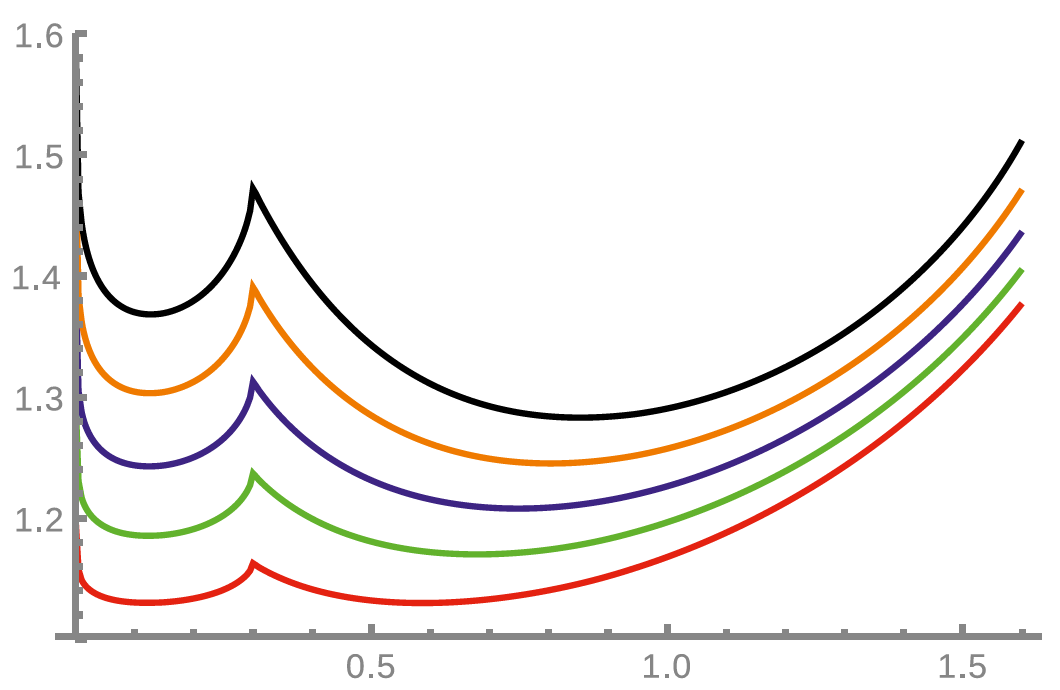
\includegraphics[scale = .25]{plot/3.png}
    \end{minipage}  
    \begin{minipage}[r]{.5\textwidth}
      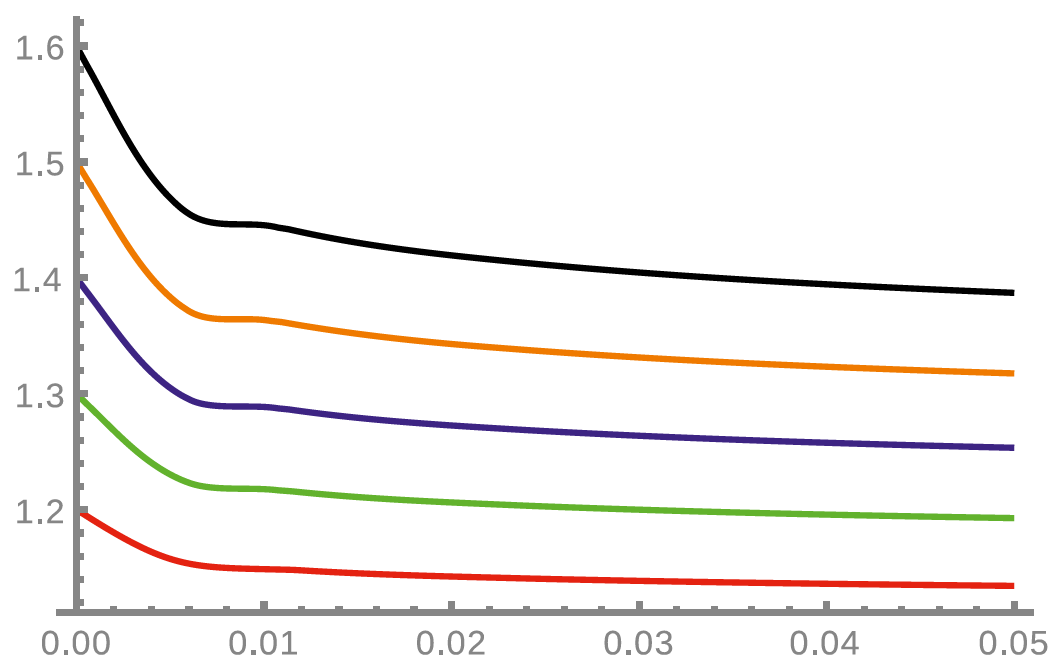
\includegraphics[scale = .25]{plot/4.png}
    \end{minipage} 
    \caption{
        Graphs of solutions to the differential equation $\leftindex[I]^C {D^{0.28}}y(t) = \sqrt{|0.3-t|} \sin(3y(t))+ 0.3t^3$
        with initial conditions $y(0) = 1.2$ (red), $y(0) = 1.3$ (green), $y(0) = 1.4$ (blue), $y(0) = 1.5$ (orange)
        and $y(0) = 1.6$ (black), plotted over the interval $[0, 1.6]$ (left) and zoom of this picture to the interval
        $[0, 0.05]$ (right). It can be observed that the graphs never meet or cross each other.
    } 
\end{figure*}
% \subsection{Terminal Value Problems For Single-Term Equations}
% A different type of problems has also received some attention recently
% Observing the state of the system at the point $t^*$ on the interval $[0, t^*]$, 
% Since the point $t^*$ at which the information is given is the end point of this interval, 
% a problem of this type is commonly referred to as a "terminal value problem".
% and it's the condition that accompany the equation is in the form of 
% \[
%     y(t^*) = \beta^*
% \]
% For the sake of simplicity, we restrict our attention to the case where one condition is imposed 
% which means we consider only differential equations of order $\alpha \in (0, 1)$, 
% now we need to see when such a terminal value problem have a unique solution. 

% If one can manage to find the solution on $[0, t^*]$ then the system's state at
% $t = 0$ is known and can be used to define a standard initial condition that then replaces
% the terminal condition, so that the new IVP can be solved on an interval
% $[0, T]$ with some $T > t^*$ 

% In the context of terminal value problems it suffices to work on the interval $[0, t^*]$. In
% this context, it is of interest to derive an analog of the integral equation formulation
% of the IVP that Lemma (6.1) provided. This result looks as follows.

% \begin{lemma}
%     Let $t^* > 0$ and $0 < \alpha < 1$, and assume $f := [0, t^*]\times \mathbb{R} \to \mathbb{R}$ to be continuous and
%     satisfies Lipschitz condition with respect to the second variable. Then the TVP
%     \begin{equation}
%         \begin{cases}
%             \leftindex[I]^C {D^{\alpha}} y(t) = f(t,y(t))
%             \\
%             T.C \Longrightarrow y(t^*) = \beta^*
%         \end{cases}
%     \end{equation}
%     Is equivalent to the weakly singular integral equation
%     \[
%         y(t) = \beta^* + \frac{1}{\Gamma(\alpha)}\int_{0}^{t^*} G(t,s)f(s,y(s)) \hquad ds
%     \]
%     Where 
%     \[
%         G(t,s)=
%         \begin{cases}
%             -(t^* - s)^{\alpha-1} & \text{ for } s>t
%             \\
%             (t-s)^{\alpha-1} - (t^* - s)^{\alpha-1} & \text{ for } s \leq t
%         \end{cases} 
%     \]
% \end{lemma}
% The substantial difference between the integral equation of Lemma (6.8) and the integral
% equation derived in Lemma (6.1) is that we now have a Fredholm integral equation of 
% Hammerstein type whereas the IVP gave rise to a Volterra equation. 

% Thus, in analogy with the corresponding results for integer order equations, 
% it would be natural to interpret the terminal condition as a boundary condition
% and not an initial condition. Hence, in contrast to the situation observed for
% first order differential equations, the TVP (6.6) is much more closely related to a boundary value problem than it is to an
% IVP.

% In spite of this difference, it is possible to provide an existence and uniqueness
% theorem for TVPs that formally coincides with the corresponding
% result for IVPs.
% \begin{theorem}
%     Under the assumptions of Lemma (6.8), the TVP (6.6) has exactly one continuous solution on $[0, t^*]$.
% \end{theorem}
% This result holds for the case of a scalar problem only, but not necessarily when
% the functions are assumed to be vector valued.

\newpage 

\subsection{Linear Fractional Differential Equations (LFDE)}
A linear FDE is an equation of form
\[
    \left(\leftindex[I]^C {D^{\alpha_m}} + a_{m-1}(t)\leftindex[I]^C {D^{\alpha_{m-1}}} + \dots + a_{1}(t)\leftindex[I]^C {D^{\alpha_{1}}} + a_{1}(t) \right) y(t) = f(t)
\]
With the conditions:
\[
    y^{(k)}(0) = \beta_k \quad,\quad k = 0,1,2,\dots,m-1
\]
\begin{theorem}[Existence And Uniqueness Of LFDE]
    If $f(t)$ is bounded on $(0, T)$ and $a_{k}(t)$ , $k = {0, 1, \dots , m-1}$ 
    are continuous functions on $[0, T]$, the equation has a unique solution.
\end{theorem}
In the particular case where the given differential equation is linear, it is often possible
to write up the solutions in closed form.
\begin{example}
    Show that 
    \[
        y(t) = \frac{1}{\Gamma(\alpha)}\int_{0}^{t} (t-s)^{\alpha-1}f(s) \hquad ds
    \]
    Solves the IVP 
    \[
        \begin{cases}
            \leftindex[I]^C {D^{\alpha}} y(t) = f(t)    \quad&,\quad m-1<\alpha<m
            \\
            I.C \Longrightarrow y^{(k)}(0) = 0 \quad&,\quad k = 0,1,2,\dots,m-1
        \end{cases}
    \]
    \textit{ \textbf{Sol.} } We apply the Laplace transform
        \begin{align*}
            \mathcal{L}\left[\leftindex[I]^C {D^{\alpha}} y(t)\right] &= \mathcal{L}[f(t)]
            \\
            s^{\alpha} Y(s) &= F(s)
            \\
            Y(s) &= s^{-\alpha}F(s)
            \\
            \mathcal{L}[y(t)] &= \mathcal{L}\left[I^{\alpha}f(t)\right]
            \\
            y(t) &= I^{\alpha}f(t) = \frac{1}{\Gamma(\alpha)}\int_{0}^{t} (t-s)^{\alpha-1}f(s) \hquad ds
        \end{align*}
\end{example}
\begin{enrichment*}{Laplace of Mittag Leffler Function }
    \[
        \mathcal{L}\left[t^{\beta-1} E_{\alpha,\beta}(\lambda t^\alpha)\right] = \frac{s^{\alpha - \beta}}{s^{\alpha}-\lambda}
    \]
\end{enrichment*}
\begin{example}
    Show that 
    \[
        y(t) = \sum_{k=0}^{m-1} \beta_k t^{k} E_{\alpha,k+1}(\lambda t^\alpha)
    \]
    Solves the IVP 
    \[
        \begin{cases}
            \leftindex[I]^C {D^{\alpha}} y(t) = \lambda y(t)    \quad&,\quad m-1<\alpha<m
            \\
            I.C \Longrightarrow y^{(k)}(0) = \beta_k \quad&,\quad k = 0,1,2,\dots,m-1
        \end{cases}
    \]
    \textit{ \textbf{Sol.} } We apply the Laplace transform
        \begin{align*}
            \mathcal{L}\left[\leftindex[I]^C {D^{\alpha}} y(t)\right] &= \lambda \mathcal{L}[y(t)]
            \\
            s^{\alpha} Y(s) - \sum_{k=0}^{m-1} s^{\alpha-k-1} y^{(k)}(0) &= \lambda Y(s)
            \\
            Y(s) &= \sum_{k=0}^{m-1} \frac{s^{\alpha-k-1}}{s^{\alpha}-\lambda} \beta_k
            \\
            \mathcal{L}[y(t)] &= \sum_{k=0}^{m-1} \mathcal{L}\left[\beta_k t^{k} E_{\alpha,k+1}(\lambda t^\alpha)\right]
            \\
            \mathcal{L}[y(t)] &= \mathcal{L}\left[\sum_{k=0}^{m-1} \beta_k t^{k} E_{\alpha,k+1}(\lambda t^\alpha)\right]
            \\
            y(t) &= \sum_{k=0}^{m-1} \beta_k t^{k} E_{\alpha,k+1}(\lambda t^\alpha)
        \end{align*}
\end{example}
In example (6.1.4) if we take special case when $m-1 = 0$ and for $\lambda = -1$. 
\[
    y(t) = \beta_0 E_{\alpha,1}(-t^\alpha)
\]
The cases $\alpha = 1$ and $\alpha = 2$
reduce to the well known statements that are the exponential function $E_{1,1}(-t) = e^{-t}$ and
the cosine $E_{2,1}(-t^2) = cos(t)$ solve the given first and second order IVPs.

This observation indicates that the solutions to the general problem of order $\alpha$ 
decay in a monotonic way for $\alpha = 1$ and exhibit persistent oscillations for $\alpha = 2$ if $\lambda$ is
a negative real number. 
And the behavior of the solution in the cases $1 < \alpha < 2$ and $0 < \alpha < 1$. 
The associated results are illustrated in Figure 2
\begin{figure*}[h]
    \begin{minipage}[l]{.5\textwidth}
      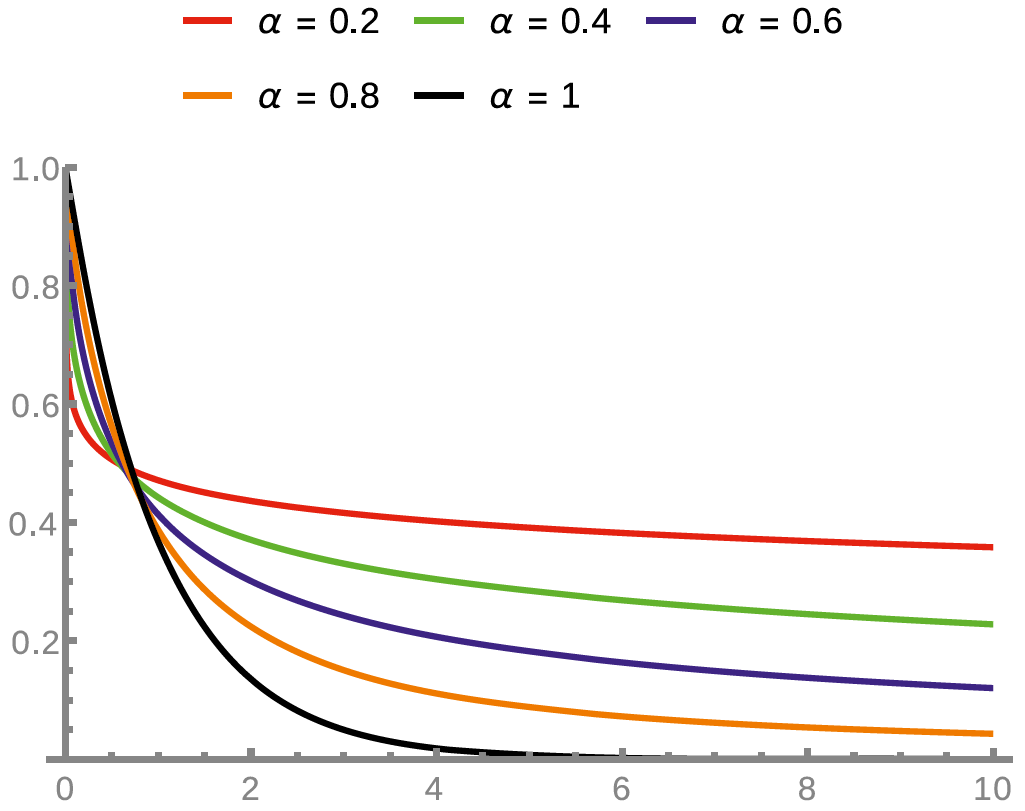
\includegraphics[scale = .25]{plot/1.png}
    \end{minipage}  
    \begin{minipage}[r]{.5\textwidth}
      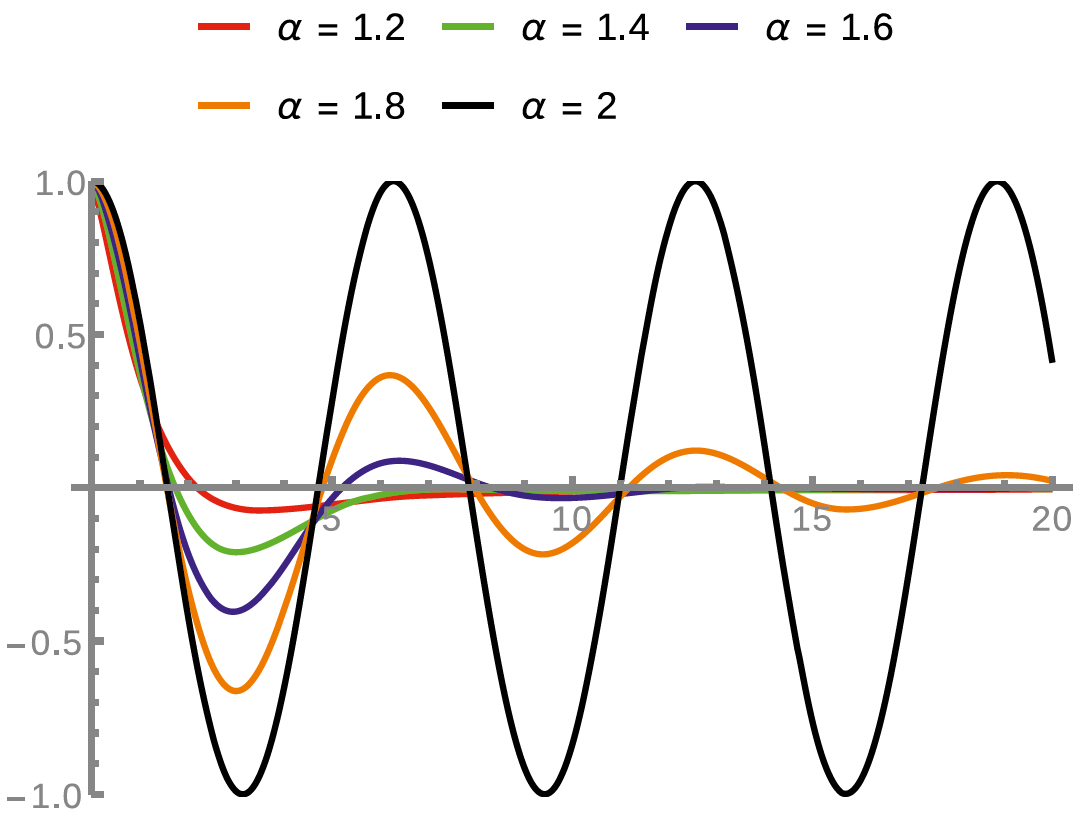
\includegraphics[scale = .25]{plot/2.png}
    \end{minipage} 
    \caption{Plots of $y(t) = E_{\alpha}(-t^\alpha)$ for various $\alpha \in (0, 1]$ (left) and $\alpha \in (1, 2]$ (right).} 
\end{figure*}

\begin{example}
    Show that 
    \[
        y(t) = \beta + t^{\alpha} \sum_{n=0}^{\infty} \frac{f^{(n)}(0)}{\Gamma(n+\alpha+1)}t^n
    \]
    Solves the IVP 
    \[
        \begin{cases}
            \leftindex[I]^C {D^{\alpha}} y(t) = f(t)    \quad,\quad 0<\alpha<1
            \\
            I.C \Longrightarrow y(0) = \beta
        \end{cases}
    \]
    \textit{ \textbf{Sol.} } We expand $f(t)$ using Taylor expansion and apply the Laplace transform
        \begin{align*}
            \mathcal{L}[\leftindex[I]^C {D^{\alpha}} y(t)] &= \mathcal{L}[f(t)]
            \\
            s^{\alpha} Y(s) - \beta s^{\alpha-1} &= \mathcal{L}\left[\sum_{n=0}^{\infty} \frac{f^{(n)}(0)}{\Gamma(n+1)}t^n\right]
            \\
            Y(s) &= \frac{\beta}{s} + \sum_{n=0}^{\infty} \frac{f^{(n)}(0)}{\Gamma(n+1)}\frac{1}{s^{\alpha}}\mathcal{L}[t^n]
            \\
            \mathcal{L}[y(t)] &= \mathcal{L}[\beta] + \sum_{n=0}^{\infty} \frac{f^{(n)}(0)}{\Gamma(n+1)}\frac{1}{s^{\alpha}}\frac{\Gamma(n+1)}{s^{n+1}}
            \\
            \mathcal{L}[y(t)] &= \mathcal{L}[\beta] + \sum_{n=0}^{\infty} f^{(n)}(0) \frac{1}{s^{n+\alpha+1}}
            \\
            \mathcal{L}[y(t)] &= \mathcal{L}[\beta] + \sum_{n=0}^{\infty} f^{(n)}(0) \mathcal{L}\left[\frac{t^{n+\alpha}}{\Gamma(n+\alpha+1)}\right]
            \\
            y(t) &= \beta + t^{\alpha} \sum_{n=0}^{\infty} \frac{f^{(n)}(0)}{\Gamma(n+\alpha+1)}t^n
        \end{align*}
\end{example}
% \newpage
\begin{example}
    Solve the in-homogeneous IVP 
    \[
        \begin{cases}
            \leftindex[I]^C {D^{\alpha}} y(t) = \lambda y(t) + Q(t)   \quad&,\quad m-1<\alpha<m
            \\
            I.C \Longrightarrow y^{(k)}(0) = \beta_k \quad&,\quad k = 0,1,2,\dots,m-1
        \end{cases}
    \]
    Where $Q \in C[0, h]$ is a given function 

    \textit{ \textbf{Sol.} } As we did previously we expand $Q(t)$ using Taylor expansion and apply the Laplace transform
    \begin{align*}
        \mathcal{L}\left[\leftindex[I]^C {D^{\alpha}} y(t)\right] &= \lambda \mathcal{L}[y(t)] + \mathcal{L}\left[\sum_{n=0}^{\infty} \frac{Q^{(n)}(0)}{\Gamma(n+1)}t^n\right]
        \\
        s^{\alpha} Y(s) - \sum_{k=0}^{m-1} s^{\alpha-k-1} y^{(k)}(0) &= \lambda Y(s) + \sum_{n=0}^{\infty} Q^{(n)}(0) s^{-n-1} 
        \\
        Y(s) &= \sum_{k=0}^{m-1} \frac{s^{\alpha-k-1}}{s^{\alpha}-\lambda} \beta_k + \sum_{n=0}^{\infty} Q^{(n)}(0) \frac{s^{-n-1} }{s^{\alpha}-\lambda}
        \\
        \mathcal{L}[y(t)] &= \sum_{k=0}^{m-1} \mathcal{L}\left[\beta_k t^{k} E_{\alpha,k+1}(\lambda t^\alpha)\right] + \sum_{n=0}^{\infty} Q^{(n)}(0) \frac{s^{\alpha-\alpha-n-1} }{s^{\alpha}-\lambda}
        \\
        \mathcal{L}[y(t)] &= \mathcal{L}\left[\sum_{k=0}^{m-1} \beta_k t^{k} E_{\alpha,k+1}(\lambda t^\alpha)\right] + \sum_{n=0}^{\infty} \mathcal{L}\left[Q^{(n)}(0) t^{\alpha+n} E_{\alpha,\alpha+n+1}(\lambda t^\alpha)\right]
        \\
        \mathcal{L}[y(t)] &= \mathcal{L}\left[\sum_{k=0}^{m-1} \beta_k t^{k} E_{\alpha,k+1}(\lambda t^\alpha)\right] + \mathcal{L}\left[\sum_{n=0}^{\infty} Q^{(n)}(0) t^{\alpha+n} E_{\alpha,\alpha+n+1}(\lambda t^\alpha)\right]
        \\
        \tag{6.7} y(t) &= \sum_{k=0}^{m-1} \beta_k t^{k} E_{\alpha,k+1}(\lambda t^\alpha) + \sum_{n=0}^{\infty} Q^{(n)}(0) t^{\alpha+n} E_{\alpha,\alpha+n+1}(\lambda t^\alpha)
        \intertext{Using Mittag Leffler function recursion relation $\displaystyle E_{\alpha,\alpha+\beta}(z) = \frac{1}{z}\left[E_{\alpha,\beta}(z) - \frac{1}{\Gamma(\beta)}\right]$}
        &= \sum_{k=0}^{m-1} \beta_k t^{k} E_{\alpha,k+1}(\lambda t^\alpha) + \sum_{n=0}^{\infty} Q^{(n)}(0) t^{\alpha+n} \frac{1}{\lambda t^\alpha}\left[E_{\alpha,n+1}(z) - \frac{1}{\Gamma(n+1)}\right]
        \\
        &= \sum_{k=0}^{m-1} \beta_k t^{k} E_{\alpha,k+1}(\lambda t^\alpha) + \frac{1}{\lambda}\sum_{n=0}^{\infty} Q^{(n)}(0) t^{n}E_{\alpha,n+1}(z) - \frac{Q(t)}{\lambda}
        \setcounter{equation}{7}
    \end{align*}
Another way using the superposition principle
\begin{enrichment*}{The Superposition Principle}
    The solution of the in-homogeneous equation can be written as the 
    sum of the solution of the homogeneous equation, and a particular 
    solution of the in-homogeneous equation.
\end{enrichment*}
We can break the problem into the following two problems
\[
    \begin{cases}
        \leftindex[I]^C {D^{\alpha}} y_h(t) = \lambda y_h(t)  \quad&,\quad m-1<\alpha<m
        \\
        I.C \Longrightarrow y_h^{(k)}(0) = \beta_k \quad&,\quad k = 0,1,2,\dots,m-1
    \end{cases}
\]
\[
    \begin{cases}
        \leftindex[I]^C {D^{\alpha}} y_p(t) = \lambda y_p(t) + Q(t)   \quad&,\quad m-1<\alpha<m
        \\
        I.C \Longrightarrow y_p^{(k)}(0) = 0 \quad&,\quad k = 0,1,2,\dots,m-1
    \end{cases}
\]
Where $y = y_h + y_p$ solves the original problem.
From example (6.3.2) we got that
\[
    y_h(t) = \sum_{k=0}^{m-1} \beta_k t^{k} E_{\alpha,k+1}(\lambda t^\alpha)
\]
Now for the second problem take Laplace Transform for it 
\begin{align*}
    \mathcal{L}\left[\leftindex[I]^C {D^{\alpha}} y_p(t)\right] &= \lambda \mathcal{L}[y_p(t)] + \mathcal{L}\left[\sum_{n=0}^{\infty} \frac{Q^{(n)}(0)}{\Gamma(n+1)}t^n\right]
    \\
    s^{\alpha} Y_p(s) &= \lambda Y_p(s) + \sum_{n=0}^{\infty} Q^{(n)}(0) s^{-n-1} 
    \\
    Y_p(s) &= \sum_{n=0}^{\infty} Q^{(n)}(0) \frac{s^{-n-1} }{s^{\alpha}-\lambda} = \sum_{n=0}^{\infty} Q^{(n)}(0) \frac{s^{\alpha-\alpha-n-1} }{s^{\alpha}-\lambda}
    \\
    \mathcal{L}[y_p(t)] &= \sum_{n=0}^{\infty} \mathcal{L}\left[Q^{(n)}(0) t^{\alpha+n} E_{\alpha,\alpha+n+1}(\lambda t^\alpha)\right]
    \\
    \mathcal{L}[y_p(t)] &= \mathcal{L}\left[\sum_{n=0}^{\infty} Q^{(n)}(0) t^{\alpha+n} E_{\alpha,\alpha+n+1}(\lambda t^\alpha)\right]
    \\
    y_p(t) &= \sum_{n=0}^{\infty} Q^{(n)}(0) t^{\alpha+n} E_{\alpha,\alpha+n+1}(\lambda t^\alpha)
\end{align*}
Adding $y_h + y_p$ we get the result (6.7)
\end{example}
\begin{enrichment*}{Duhamel's Principle}
    If one can solve an IVP for a homogeneous linear differential equation then an in-homogeneous linear differential equation can be solved as well.
\end{enrichment*} 
\newpage
\subsection{Nonlinear Equations}
Now we will discuss One of the methods to solve Nonlinear FDE which is The Adomian Decomposition Method

The Adomian method applied to the ordinary and partial differential equations of integer order was extended 
also to the case of FDE.
\subsubsection{The Adomian Decomposition Method (ADM)}
Before we talk about how to solve FDE using ADM let us first see how it work 

Consider the problem
\begin{equation}
    \begin{cases}
        \displaystyle \pdv{u(x,t)}{t} + L(u(x,t)) + N(u(x,y)) = g(x,t)
        \\
        I.C \Longrightarrow \displaystyle u(x,0) = \phi(x)
    \end{cases}
\end{equation}
This is nonlinear partial differential equation of integer order where $L(u(x,t))$ is the linear part and $N(u(x,t))$ is the non-linear part
We will discuss it's solution by ADM
\\
Now, Integrate (6.8) from $0 \to t$
\begin{equation}
    u(x,t) = \phi(x) - \int_{0}^{t} L(u(x,s)) \hquad ds  - \int_{0}^{t} N(u(x,s)) \hquad ds  + \int_{0}^{t} g(x,s) \hquad ds
\end{equation}
Set
\begin{equation}
    u(x,t) = \sum_{n=0}^{\infty} u_n(x,y)
\end{equation}
\begin{equation}
    N(u(x,t)) = \sum_{n=0}^{\infty} A_n(x,y)
\end{equation}
Where $A_0,A_1,A_2,\dots$ are \textbf{Adomian Polynomials} defined as:
\[
    A_n(x,y) = \frac{1}{n!} \dv[n]{}{\lambda} \left( N \left( \sum_{j=0}^{n}\lambda^j u_j \right) \right)
\]
Substitute equations (6.10),(6.11) into (6.9) we get
\begin{equation*}
    u(x,y) = \sum_{n=0}^{\infty}u_n(x,t) = \phi(x) + \int_0^t g(x,s) \hquad ds - \int_0^t L \left(\sum_{n=0}^{\infty}u_n(z,t)\right)  - \int_0^t \sum_{n=0}^{\infty}A_n(x,s) \hquad ds
\end{equation*}
Now,
\begin{align*}
    u_0 & = \phi(x) + \int_0^t g(x,s) \hquad ds                 \\
    u_1 & = -\int_0^t L(u_0) \hquad ds - \int_0^t A_0 \hquad ds         \\
    u_2 & = -\int_0^t L(u_1) \hquad ds - \int_0^t A_1 \hquad ds         \\
    \vdots                                               \\
    u_n & = -\int_0^t L(u_{n-1}) \hquad ds - \int_0^t A_{n-1} \hquad ds
\end{align*}
\[
    \therefore u(x,t) = \sum_{n=0}^{\infty} u_n(x,y) = u_0 + u_1 + u_2 + \dots
\]
This will get the solution for the problem (6.8)
\newpage
Note that The Adomian Decomposition Method (ADM)
is a numerical technique used to approximate solutions
of differential equations.
Whether ADM converges or diverges depends on the
specific problem and how it is applied.
The convergence and divergence of ADM can be
influenced by several factors, including the
complexity of the problem, the choice of the
decomposition functions, and the behavior of
the nonlinear terms in the differential equation.

\begin{example}
    Solve the nonlinear differential equation using ADM
    \begin{equation}
        \begin{cases}
            \displaystyle \frac{\partial u(x,t)}{\partial t} = x^2 - \frac{1}{4}\left( \frac{\partial u(x,t)}{\partial x} \right)^2
            \\
            I.C \Longrightarrow \displaystyle u(x,0) = 0
        \end{cases}
    \end{equation}
    \textit{ \textbf{Sol.} } Set
    \begin{align*}
        u(x,t) & = \sum_{n=0}^{\infty} u_n(x,t)
        \\
        N(u)   & = \sum_{n=0}^{\infty} A_n(x,t)
    \end{align*}
    Where $N(u)$ represents the nonlinear form of $u$ 
    
    In our case in equation (6.12) $\displaystyle N(u) = \left(\frac{\partial u}{\partial x}\right)^2$
    \begin{align*}
        A_n(x,t) & = \left[\frac{1}{n!} \frac{d^n}{d \lambda^n} N\left(\sum_{i=0}^{n}  \lambda^i u_i(x,t)\right)\right]_{\lambda = 0}
        \\
        A_n(x,t) & = \left[\frac{1}{n!} \frac{d^n}{d \lambda^n} \left(\sum_{i=0}^{n}  \lambda^i \frac{\partial u_i(x,t)}{\partial x}\right)^2\right]_{\lambda = 0}
    \end{align*}
    Integrating equation (6.12) from $0 \to t$
    \[
        u(x,t) = \sum_{n=0}^{\infty} u_n(x,t)  = x^2t - \frac{1}{4} \int_{0}^{t}\sum_{n=0}^{\infty} A_n(x,\theta) \hquad d\theta
    \]
    Now we get $A_0$,$A_1$,$A_2,\dots$
    \begin{align*}
        A_0(x,\theta) & = \left[\sum_{i=0}^{0}  \lambda^i \frac{\partial u_i(x,\theta)}{\partial x}^2\right]_{\lambda = 0} = \left(\frac{\partial u_0(x,\theta)}{\partial x}\right)^2
        \\
        A_1(x,\theta) & = \left[\frac{d}{d \lambda} \left(\sum_{i=0}^{1}  \lambda^i \frac{\partial u_i(x,\theta)}{\partial x}\right)^2\right]_{\lambda = 0}
        \\
                      & = \left[\frac{d}{d \lambda} \left(\frac{\partial u_0(x,\theta)}{\partial x} + \lambda \frac{\partial u_1(x,\theta)}{\partial x}\right)^2\right]_{\lambda = 0}
        \\
                      & =2\left[\left(\frac{\partial u_0(x,\theta)}{\partial x} + \lambda \frac{\partial u_1(x,\theta)}{\partial x}\right)\frac{\partial u_1(x,\theta)}{\partial x}\right]_{\lambda = 0} = 2\frac{\partial u_0(x,\theta)}{\partial x} \frac{\partial u_1(x,\theta)}{\partial x}
        \\
        A_2(x,\theta) & =\left[\frac{1}{2!} \frac{d^2}{d \lambda^2} \left(\sum_{i=0}^{2}  \lambda^i \frac{\partial u_i(x,\theta)}{\partial x}\right)^2\right]_{\lambda = 0}
        \\
                      & = \left[\frac{1}{2} \frac{d^2}{d \lambda^2} \left(\frac{\partial u_0(x,\theta)}{\partial x} + \lambda \frac{\partial u_1(x,\theta)}{\partial x} + \lambda^2 \frac{\partial u_2(x,\theta)}{\partial x}\right)^2\right]_{\lambda = 0}
        \\
                      & = \left(\frac{\partial u_1(x,\theta)}{\partial x}\right)^2 + 2 \left(\frac{\partial u_0(x,\theta)}{\partial x}\frac{\partial u_2(x,\theta)}{\partial x}\right)
        \\
        A_3(x,\theta) & = 2\frac{\partial u_1(x,\theta)}{\partial x}\frac{\partial u_2(x,\theta)}{\partial x} + 2\frac{\partial u_0(x,\theta)}{\partial x} \frac{\partial u_3(x,\theta)}{\partial x}
    \end{align*}
    Now because
    \[
        u_0 + u_1 + u_2 + \dots = u(x,t) = x^2t - \frac{1}{4}\int_{0}^{t}[A_0+A_1+A_2+\dots] \hquad d\theta
    \]
    Then
    \begin{align*}
        u_0 & = x^2t
        \\
        u_1 & = -\frac{1}{4}\int_{0}^{t}A_0d\theta = -\frac{1}{4}\int_{0}^{t}\left(\frac{\partial u_0(x,\theta)}{\partial x}\right)^2 = -\int_{0}^{t} x^2 \theta^2 d\theta = \frac{-1}{3}x^2t^3
        \\
        u_2 & = \frac{2}{15} x^2t^5
        \\
        u_3 &= \frac{-17}{315} x^2t^7 
        \\
        \vdots
    \end{align*}
    \[
        u(x,t) = x^2 \left[t-\frac{1}{3}t^3 + \frac{2}{15} t^5 - \frac{17}{315} t^7 \dots\right] = x^2 \tanh(t)
    \]
\end{example}
\begin{figure}[b]
    \begin{enrichment}{George Adomian}{Chars/adom.jpg}{2.4}{.8}{.17}
        George Adomian (March 21, 1922 – June 17, 1996)
        was an American mathematician of Armenian descent
        who developed the Adomian decomposition method (ADM)
        for solving nonlinear differential equations,
        both ordinary and partial.
        The method is explained among other places
        in his book \textit{\textbf{"Solving Frontier Problems in Physics:
                The Decomposition Method"}}.
        He was a faculty member at the University of Georgia
        (UGA) from 1966 through 1989. While at UGA,
        he started the Center for Applied Mathematics.
        Adomian was also an aerospace engineer.
    \end{enrichment}
\end{figure}
\newpage
\subsubsection{Decomposition Of Nonlinear FDE}
We consider the following nonlinear FDE 
\begin{equation}
    \begin{cases}
        \displaystyle \leftindex[I]^C {D^{\alpha}} y(t) + L(y(t)) + N(y(t)) = f(t)
        \\
        I.C \Longrightarrow \displaystyle y^{(k)}(0) = \beta_k \quad,\quad k=0,1,2,\dots,m-1 
    \end{cases}
\end{equation}
We apply the Laplace Transform to the equation
\[
    \mathcal{L}[\leftindex[I]^C {D^{\alpha}} y(t)] = s^{\alpha} Y(s) - \sum_{k=0}^{m-1} s^{\alpha-k-1} y^{(k)}(0)
\]
We use the following decomposition of $y(t)$
\[
    y(t) = \sum_{n=0}^{\infty} y_n(t)
\]
And 
\[
    N(y(t)) = \sum_{n=0}^{\infty} A_n
\]
Where $A_n$ are Adomian polynomials

The equation (6.13) become 
\[
    \mathcal{L}\left[\sum_{n=0}^{\infty} y_n(t)\right] = \sum_{k=0}^{m-1} \frac{\beta_k}{s^{k+1}} - \frac{1}{s^{\alpha}} \mathcal{L}\left[L\left(\sum_{n=0}^{\infty} y_n(t)\right)\right] - \frac{1}{s^{\alpha}}\mathcal{L}\left[\sum_{n=0}^{\infty} A_n\right] + \frac{1}{s^{\alpha}}\mathcal{L}\left[f(t)\right]
\]
Now we can get 
\begin{align*}
    Y_0 &= \mathcal{L}\left[y_0\right] = \sum_{k=0}^{m-1} \frac{\beta_k}{s^{k+1}} + \frac{1}{s^{\alpha}}\mathcal{L}\left[f(t)\right]
    \\
    Y_1 &= \mathcal{L}\left[y_1\right] = - \frac{1}{s^{\alpha}} \mathcal{L}\left[L\left(y_0(t)\right)\right] - \frac{1}{s^{\alpha}}\mathcal{L}\left[ A_0\right]
    \\
    Y_2 &= \mathcal{L}\left[y_2\right] = - \frac{1}{s^{\alpha}} \mathcal{L}\left[L\left(y_1(t)\right)\right] - \frac{1}{s^{\alpha}}\mathcal{L}\left[ A_1\right]
    \\
    \vdots
    \\
    Y_n &= \mathcal{L}\left[y_n\right] = - \frac{1}{s^{\alpha}} \mathcal{L}\left[L\left(y_{n-1}(t)\right)\right] - \frac{1}{s^{\alpha}}\mathcal{L}\left[ A_{n-1}\right]
\end{align*}
\begin{example}
    Solve the nonlinear FDE using the Adomian decomposition method
    \[
        \begin{cases}
            \displaystyle \leftindex[I]^C {D^{\alpha}} y(t) = t + y^2 \quad,\quad 1<\alpha \leq 2
            \\
            I.C \Longrightarrow \displaystyle y(0) = 0 \quad,\quad y^{(1)}(0) = 1
        \end{cases}
    \]
    \textit{ \textbf{Sol.} } In order to solve the equation we apply the Laplace transform
    \begin{align*}
        \mathcal{L}\left[\leftindex[I]^C {D^{\alpha}} y(t)\right] &= \mathcal{L}\left[t + y^2\right]
        \\
        s^{\alpha} Y(s) - s^{\alpha-1}y(0) - s^{\alpha-2} y^{(1)}(0) &= \mathcal{L}\left[t + y^2\right]
        \\
        s^{\alpha} Y(s) - s^{\alpha-2} &= \mathcal{L}\left[t + y^2\right]
    \end{align*}
    So that, for the decomposition
    \[
        y(t) = \sum_{n=0}^{\infty} y_n(t)
    \]
    We obtain
    \[
        Y(s) = \sum_{n=0}^{\infty} Y_n(s) \quad , \quad t+y^2 = \sum_{n=0}^{\infty} A_n
    \]
    The Adomian polynomials $A_n$ are 
    \[
        A_0 = t + y_0^2 \quad,\quad A_1 = 2y_0y_1 \quad,\quad A_2 = y_1^2 + 2y_0y_2 \quad,\quad A_2 = 2y_1y_2 + 2y_0y_3 \quad,\dots
    \]
    \[
        Y_0 = \frac{1}{s^2} \quad\Longrightarrow\quad y_0 = t \quad\Longrightarrow\quad A_0 = t+t^2
    \]
    \[
        Y_1 = \frac{1}{s^\alpha}\mathcal{L}\left[A_0\right] \quad\Longrightarrow\quad y_1 = \frac{t^{\alpha+1}}{\Gamma(\alpha+2)} + 2\frac{t^{\alpha+2}}{\Gamma(\alpha+3)} \quad\Longrightarrow\quad A_1 = 2y_0y_1
    \]
    And so on 
    \[
        y(t) = y_0 + y_1 + y_2 + \dots
    \]
\end{example}


\subsection{Fractional Systems of Differential Equations}
Solving System of FDE is not very different from solving single FDE 
there are Linear Systems which can be solved using Laplace Transform 
and we will show example of them and there are Nonlinear Systems
which can be solved by Method of Successive Approximations and
The Adomian Decomposition Method

\begin{example}
    Solve the system of FDE
    \[
        \begin{cases}
            \displaystyle \leftindex[I]^C {D^{\alpha}} x(t) = \leftindex[I]^C {D^{\beta}} y(t) + 1  \quad,\quad 0<\alpha<1
            \\
            \displaystyle \leftindex[I]^C {D^{\beta}} y(t) = 2\leftindex[I]^C {D^{\alpha}} x(t) - 1 \quad,\quad 0<\beta<1
            \\
            I.C \Longrightarrow x(0) = 1 \quad,\quad y(0) = 1
        \end{cases}
    \]
    \textit{ \textbf{Sol.} } We apply the Laplace Transform method
    \[
        \begin{cases}
            \displaystyle \mathcal{L}\left[\leftindex[I]^C {D^{\alpha}} x(t) \right]= \mathcal{L}\left[\leftindex[I]^C {D^{\beta}} y(t)\right] + \mathcal{L}\left[1\right]
            \\
            \displaystyle \mathcal{L}\left[\leftindex[I]^C {D^{\beta}} y(t) \right]= 2\mathcal{L}\left[\leftindex[I]^C {D^{\alpha}} x(t)\right] - \mathcal{L}\left[1\right]
        \end{cases}
    \]
    We obtain the system
    \[
        \begin{cases}
            \displaystyle s^\alpha X(s) - s^{\alpha-1} = s^\beta Y(s) - s^{\beta-1} + \frac{1}{s}
            \\
            \displaystyle s^\beta Y(s) - s^{\beta-1} = 2s^\alpha X(s) - 2s^{\alpha-1} - \frac{1}{s}
        \end{cases}
    \]
    With the solution:
    \[
        \begin{cases}
            \displaystyle X(s) = \frac{1}{s}
            \\\\
            \displaystyle Y(s) = \frac{1}{s} - \frac{1}{s^{\beta+1}}
        \end{cases}
    \]
    Take the Laplace inverse we get the solution for the original system
    \[
        \begin{cases}
            \displaystyle x(t) = 1 
            \\\\
            \displaystyle y(t) = 1 - \frac{t^{\beta}}{\Gamma(\beta+1)}
        \end{cases}
    \]
\end{example}                     % Fractional Differential Equations Part
\section{Applications Of Fractional Calculus}
Fractional differential equations and integral equations appear in several physical systems
In this section we will review some of their applications.


\subsection{Abel's Fractional Integral Equation Of Tautochrone}
The Abel's problem is to find a curve where the time that takes a ball to reach the bottom of the curve is same irrespective 
of the position of release of ball in friction less system. 

\begin{figure*}[h]
    \hspace*{1cm}
    \begin{minipage}[l]{.5\textwidth}
        \begin{tikzpicture}
            \draw[->] (0,0) -- (0,3);
            \draw[->] (0,0) -- (pi+1,0);
            \draw[red,domain=pi:2*pi,samples=50] plot ({-(\x - sin(\x r))+2*pi},{-(1 - cos(\x r))+2});
            
            \filldraw [blue] (0,2) circle (2pt);
            \filldraw [green] (.5,1.07) circle (2pt);
            \filldraw [yellow] (1.3,.47) circle (2pt);
            \filldraw [red!50!blue] (2,.17) circle (2pt);
            \node at (2, 2) {$t = t_i$};
        \end{tikzpicture}
    \end{minipage}  
    \begin{minipage}[r]{.5\textwidth}
        \begin{tikzpicture}
            \draw[->] (0,0) -- (0,3);
            \draw[->] (0,0) -- (pi+1,0);
            \draw[red,domain=pi:2*pi,samples=50] plot ({-(\x - sin(\x r))+2*pi},{-(1 - cos(\x r))+2});
            
            \filldraw [blue] (pi,0) circle (2pt);
            \filldraw [green] (pi,0) circle (2pt);
            \filldraw [yellow] (pi,0) circle (2pt);
            \filldraw [red!50!blue] (pi,0) circle (2pt);
            \node at (2, 2) {$t = t_f$};
        \end{tikzpicture}
    \end{minipage} 
\end{figure*}

Let $S$ be the arc length measured along curve $C$ from point $O$ to an arbitrary point $Q$ on $C$
\begin{center}
    \begin{tikzpicture}
        \draw[->] (0,0) -- (0,3);
        \draw[->] (0,0) -- (pi+1,0);
        \draw[red,domain=pi:2*pi,samples=50] plot ({-(\x - sin(\x r))+2*pi},{-(1 - cos(\x r))+2});
        
        \draw[green,domain=pi:1.52*pi,samples=50] plot ({-(\x - sin(\x r))+2*pi},{-(1 - cos(\x r))+2});
        \filldraw [blue] (.5,1.07) circle (2pt);
        \node at (1.5, .8) {$S$};
        \node at (pi, -.2) {$O$};
        \node at (-.2, 2) {$P$};
        \node at (.5, .5) {$C$};
        \node at (.8,1.2) {$Q$};
    \end{tikzpicture}
\end{center}
The gain in Kinetic Energy while the ball descends is loss in the
potential energy and is given by
\begin{align*}
    \frac{1}{2}m \left(\dv{s}{t}\right)^2 &= mg(y-\eta)
    \\
    ds &= - \sqrt{2g (y-\eta)} \hquad dt
\end{align*}
The negative square root indicates that the distance (arc-length) decreases as the
time increases.
The equation thus to be solved is
\[
    dt = -\frac{1}{\sqrt{2g (y-\eta)}} \hquad ds
\]
The time of decent from $P$ to $O$ is $T$ , which is constant thus
\[
    T = -\frac{1}{\sqrt{2g}} \int_{P}^{O}\frac{1}{\sqrt{(y-\eta)}} \hquad ds
\]
Now taking, the arc length as a function $s = h(\eta)$ , where $h$ depends on the shape
of $C$. \\
We can write in differential form the curve as $\displaystyle ds = \dv{}{\eta}h(\eta) \hquad d\eta $ , so this substitution gives
\begin{align*}
    T &= -\frac{1}{\sqrt{2g}} \int_{y}^{0}\frac{1}{\sqrt{(y-\eta)}} \dv{}{\eta}h(\eta) \hquad d\eta
    \\
    \sqrt{2g} T &= \int_{0}^{y}(y-\eta)^{-\frac{1}{2}} \dv{}{\eta}h(\eta) \hquad d\eta
\end{align*}
Meaning that the integral of right hand side of above, when a constant will be solution to get
constant time of decent $(T)$. In the above expression rewriting the integral of right hand side as
\[
    \sqrt{2g} T = \int_{0}^{y}(y-t)^{-\frac{1}{2}} f(t) \hquad dt
\]
This is Abel's integral equation where $\displaystyle f(t) = \dv{}{t}h(t)$.
\\
Abel solved this problem using convolutions and Laplace transforms but using fractional calculus 
we can see a much quicker solution if we divide both sides by $\Gamma(\frac{1}{2})$ which is equal to $\sqrt{\pi}$
we get this 
\[
    \frac{\sqrt{2g}}{\sqrt{\pi}} T = \frac{1}{\Gamma(\frac{1}{2})} \int_{0}^{y}(y-t)^{-\frac{1}{2}} f(t) \hquad dt
\]
We notice that the integral in the right hand side is the semi integral of $f(t)$
\\
In terms of fractional order Integral, this equation can be written as
\[
    \sqrt{\frac{2g}{\pi}} T = I^{\frac{1}{2}}f(t)
\]
Now by taking half derivative of RL type for both sides we get 
\[
    D^{\frac{1}{2}} \sqrt{\frac{2g}{\pi}} T = f(t)
\]
Thus 
\[
    f(t) = \sqrt{\frac{2g}{\pi}} \frac{T}{\sqrt{t}}
\]
Doing algebraic manipulation the following is obtained.
\[
    f(y) = \dv{}{y} h(y) = \dv{s}{y} = \frac{\sqrt{dx^2 + dy^2}}{dy} = \sqrt{1+ \left(\dv{x}{y}\right)^2}
\]
Thus
\begin{align*}
    \dv{x}{y} &= \sqrt{f(y)^2-1}
    \\
    x &= \int_{0}^{y} \sqrt{\frac{2g T^2}{\pi^2 \eta} - 1} \hquad d\eta + C
\end{align*}
If we make the curve start from (0,0)

\begin{center}
    \begin{tikzpicture}
        \draw[->] (0,0) -- (0,3);
        \draw[->] (0,0) -- (3,0);
        \draw[red,domain=0:pi,samples=50] plot ({\x - sin(\x r)},{1 - cos(\x r)});
    \end{tikzpicture}
\end{center}

We can get that $C = 0$

Now Substitute \(
    \begin{cases}
        \displaystyle a = \frac{2g T^2}{\pi^2}
        \\
        \displaystyle \eta = 2a \hquad sin^2(\xi)
        \\
        \displaystyle d\eta = 4a \hquad sin(\xi) \hquad cos(\xi) \hquad d\xi
        \\
        \displaystyle 0 \to \beta
        \\
        \displaystyle \beta = sin^{-1}\left(\sqrt{\frac{y}{2a}}\right)
    \end{cases}
    \)
\\
We get 
\begin{align*}
    x &= 4a \int_{0}^{\beta} \sqrt{\csc^2(\xi) - 1} \hquad sin(\xi) \hquad cos(\xi) \hquad d\xi
    \\
    x &= 4a \int_{0}^{\beta} \cot(\xi) \hquad sin(\xi) \hquad cos(\xi) \hquad d\xi
    \\
    x &= 4a \int_{0}^{\beta} cos^2(\xi) \hquad d\xi
\end{align*}
Thus we obtain
\begin{align*}
    x &= 2a\left(\beta - \frac{1}{2}\sin(2\beta)\right)
    \\
    y &= 2a\sin^2(\beta)
\end{align*}
Put $\theta = 2\beta$ and we know that $\displaystyle a=\frac{gT^2}{\pi^2}$ we obtain
\begin{align*}
    x &= a\left(\theta - \sin(\theta)\right)
    \\
    y &= a(1-\cos(\theta))
\end{align*}
The parametric equation of the cycloid
\\
The cycloid is a curve you get when you roll a circle and focus on a point 
\begin{center}
    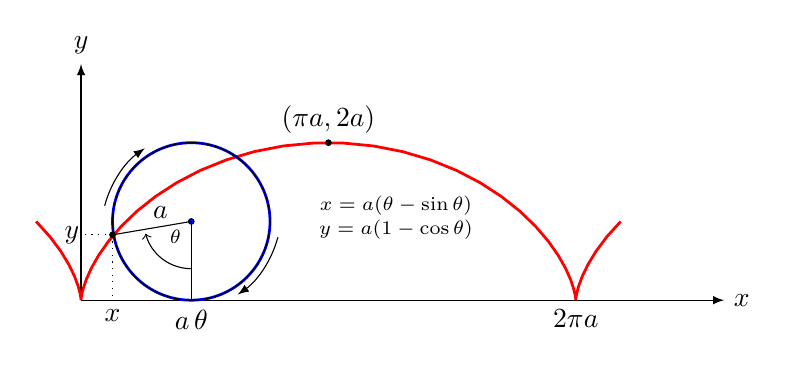
\begin{tikzpicture}
    \coordinate (O) at (0,0);
    \coordinate (A) at (0,3);
    \def\r{1} % radius
    \def\c{1.4} % center
    \coordinate (C) at (\c, \r);
  
  
    \draw[-latex] (O) -- (A) node[anchor=south] {$y$};
    \draw[-latex] (O) -- (2.6*pi,0) node[anchor=west] {$x$};
    \draw[red,domain=-0.5*pi:2.5*pi,samples=50, line width=1] 
         plot ({\x - sin(\x r)},{1 - cos(\x r)});
    \draw[blue, line width=1] (C) circle (\r);
    \draw[] (C) circle (\r);
  
    % coordinate x 
    \def\x{0.4} % coordinate x
    \def\y{0.83} % coordinate y
    \def\xa{0.3} % coordinate x for arc left
    \def\ya{1.2} % coordinate y for arc left
    \coordinate (X) at (\x, 0 );
    \coordinate (Y) at (0, \y );
    \coordinate (XY) at (\x, \y );
  
    \node[anchor=north] at (X) {$x$} ;
  
    % draw center of circle
    \draw[fill=blue] (C) circle (1pt);
  
    % draw radius of the circle
    \draw[] (C) -- node[anchor=south] {\; $a$} (XY);
  
    % bottom of circle, radius to the bottom
    \coordinate (B) at (\c, 0);
    \draw[] (C) -- (B) node[anchor=north] {$a \, \theta$};
  
    % projections of point XY
    \draw[dotted] (XY) -- (X);
    \draw[dotted] (XY) -- (Y) node[anchor=east, xshift=1mm] {$\quad y$};
  
    % arc theta
    % start arc
    \coordinate (S) at (\c, 0.4);
    \draw[->] (S) arc (-90:-165:0.6);
    \node[xshift=-2mm, yshift=-2mm] at (C) {\scriptsize $\theta$};
  
    % arc above
    \coordinate (AA) at (\xa, \ya);
    \draw[-latex, rotate=25] (AA) arc (-220:-260:1.3);
  
    % arc below
    \def\xb{2.5} % coordinate x for arc bottom
    \def\yb{0.8} % coordinate y for arc bottom
    \coordinate (AB) at (\xb, \yb);
    \draw[-latex, rotate=-10] (AB) arc (-5:-45:1.3);
  
  
  
    % XY dot
    \draw[fill=black] (XY) circle (1pt);
  
  
    % top label
    \coordinate (T) at (pi, 2);
    \node[anchor=south] at (T)  {$(\pi a, 2 a )$} ;
    \draw[fill=black] (T) circle (1pt);
  
    % equations
    \coordinate (E) at ( 4,1.2);
    \coordinate (F) at ( 4,0.9);
    \node[] at (E) {\scriptsize $x=a(\theta - \sin \theta)$};
    \node[] at (F) {\scriptsize $y=a(1 - \cos \theta)$};
  
    % label 2pi a
    \coordinate (TPA) at (2*pi, 0);
    \node[anchor=north] at (TPA) {$2 \pi a$};
  
  
    \end{tikzpicture}
  \end{center}
Cycloid is the tautochrone.
\\
A point be mentioned about the cycloid curve shape is that this is too a
curve for brachistochrone problem solved by Bernoulli. That is determination of
shape of the curve giving minimum time of descent. Therefore, the constant time
$T$ is also minimum time of descent in a cycloid.

\subsection{Viscoelasticity}
Viscoelasticity is a the field that interested in studying the property of materials that exhibit 
both viscous and elastic characteristics when undergoing deformation
and it seems to be the field of the most extensive applications
of fractional differential and integral operators.

There are two main quantities in viscoelasticity, a stress $\sigma(t)$ and a strain $\epsilon(t)$.
\\
The relationships between stress and strain for solids(Hooke’s law)
\[
\sigma(t) = E\epsilon(t)   
\]
And for Newtonian fluids
\[
\sigma(t) = \eta \dv{\epsilon(t)}{t}   
\]
Where $E$ and $\eta$ are constants. These functions satisfy the fractional
differential equations
\[
    D^\alpha \sigma(t) = \frac{\Gamma(1-\alpha) t^{-\alpha}}{\Gamma(1-2\alpha)} \sigma(t)
\]
\[
    D^\alpha \epsilon(t) = \Gamma(1+\alpha)t^{-\alpha} \epsilon(t)
\]
\newpage
\subsection{Fractional Damped Motion}
Consider a ball falling freely under gravity in viscous fluid having constituent equation as 
\[
    D^1 v(t) + D^{\alpha}v(t) + v(t) = 1
\]
With initial condition $v(0) = 0$ 
\\
Using Laplace Transformation
\begin{align*}
    sV(s) + s^{\alpha}V(s) + V(s) &= \frac{1}{s}
    \\
    (s + s^{\alpha} + 1)V(s) &= \frac{1}{s}
    \\
    V(s) &= \frac{1}{s(s + s^{\alpha} + 1)}
    \\
    &= \frac{\left[1-(-s^{-1}-s^{\alpha-1})\right]^{-1}}{s^2}
\end{align*}
Expanding numerator as binomial series, where $(s^{-1} + s^{\alpha-1}) < 1$ and $\alpha < 1$, for
large $s$ 
\\
The expansion is
\begin{align*}
    V(s) &= \sum_{n=0}^{\infty}(-1)^n \sum_{r=0}^{\infty} {n \choose r} \frac{1}{s^{n+2-r\alpha}}
    \intertext{Using Laplace Inverse}
    v(t) &= \sum_{n=0}^{\infty}(-1)^n \sum_{r=0}^{\infty} {n \choose r} \frac{t^{n+1-r\alpha}}{\Gamma(n+2-r\alpha)}
\end{align*}

Consider another fractional damping system where the inertia plays negligible role
given by
\[
    D^{\frac{1}{3}} x(t) + x(t) = f(t) \quad,\quad x(0)= 0
\]
And $f(t) = H(t)$ Heaviside's step function
\\
The Laplace transforms gives
\[
    X(s) = \frac{1}{s(1+s^{\frac{1}{3}})} = \frac{\left[1-(-s^{-\frac{1}{3}})\right]^{-1}}{s^{\frac{4}{3}}}
\]
With $|s|<< 1$ , the above is expanded as the following series
\[
    X(s) = \sum_{n=4}^{\infty} \frac{(-1)^n}{s^{\frac{n}{3}}}
\]
And Using Laplace Inverse the temporal expression for above fractional dynamics equation's solution is
\[
    x(t) = \sum_{n=4}^{\infty}(-1)^n \frac{t^{\frac{n}{3}-1}}{\Gamma(\frac{n}{3})}
\]


\subsection{Fractional Diffusion Equations}
Fractional differential equations are applied to models in relaxation and
diffusion problems. Fractional calculus is used to formulate and to solve
different physical models allowing a continuous transition from relaxation
to oscillation phenomena. An application to an anomalous diffusion process
demonstrates that the method used is also useful for more than one
independent variable

\newpage

\subsection{Fractional Order Multipoles In Electromagnetism}
It is well known that the axial multipole expansion of the
electrostatic potential of electric charge distribution in three
dimensions is
\[
    \Phi_n(r) = \frac{q}{4\pi \epsilon} \sum_{n=0}^{\infty} \frac{1}{r^{n+1}} P_n(\cos(\theta))
\]
Where 
\begin{itemize}
    \item $q$ is the called electric monopole moment
    \item $\epsilon$ is constant permittivity of the homogeneous isotropic medium
    \item $r = \sqrt{x^2 + y^2 + z^2}$
    \item $P_n(\cos(\theta))$ is the Legendre function of $n$ degree.     
\end{itemize}
The electrostatic potential functions for monopole $(2^0)$, dipole $(2^1)$, and 
quadrupole $(2^2)$ are respectively, given by
\begin{align}
    \notag \Phi_0(r) &= \frac{q}{4\pi \epsilon} \frac{1}{r}
    \\
    \Phi_1(r) &= \frac{q}{4\pi \epsilon} \frac{\cos(\theta)}{r^{2}} 
    \\
    \notag \Phi_2(r) &= \frac{q}{4\pi \epsilon} \frac{1}{r^{3}} P_n(\cos(\theta))
\end{align}
The scientist Nader Engheta generalized the idea of the integer order multipoles 
related to powers of 2 to the fractional order multipoles that are called $2^{\alpha}$-poles

He obtained the potential function for $2^{\alpha}$-poles $(0 < \alpha < 1)$ along
the $z-axis$, in terms of the Riemann-Liouville fractional derivatives in the form
\begin{equation}
    \Phi_{2^{\alpha}}(r) = \frac{q l^{\alpha}}{4\pi \epsilon} \leftindex[I]_{-\infty}{D_z^{\alpha}} \frac{1}{r}
\end{equation}
Where $l$ is a constant with dimension of length so that the usual
dimension of the resulting volume charge density is Coulomb/$m^3$

Evaluating the fractional derivative (7.2) yields the following result for the electrostatic potential
\begin{equation}
    \Phi_{2^{\alpha}}(r) = \frac{q l^{\alpha} \Gamma(\alpha+1)}{4\pi\epsilon r^{\frac{(\alpha+1)}{2}}}  P_{\alpha}\left(-\frac{z}{r}\right)
\end{equation}
Where $P_{\alpha}(x)$ is the Legendre function of the first kind and of fractional degree $\alpha$.
\\
When $\alpha = 0$, $\alpha = 1$ , and $\alpha = 2$, the potentials (7.3) reduce to those given by (7.1).




\vspace*{\fill}


\section*{\LARGE Conclusion}
It's pretty clear why there hasn't been any significant 
applications of fractional Calculus in the past 300 years 
computing these without a computer is pretty tedious and difficult 

Although fractional calculus doesn't have that many application it demo an extremely important lesson in mathematics and that's 
to try to break the rules and see what happens this is what led to the discovery of so many things like complex numbers 
when people tried to take the square root of negative numbers 

And although it's hard to see fractional derivatives geometrically it's quite a fascinating topic                    % Application Part
\newpage
\begin{thebibliography}{9}
    \bibitem{a} \textbf{Theory of Fractional Calculus and their Applications} 
    \\\textit{by Hussein A.H. Salem}
    \bibitem{h} \textbf{Fractional Differential Equations: An Introduction to Fractional Derivatives, Fractional Differential Equations, to Methods of Their Solution and Some of Their Applications }
    \\\textit{by Igor Podlubny}
    \bibitem{L} \textbf{The Analysis of Fractional Differential Equations: An Application-Oriented Exposition Using Differential Operators of Caputo Type}
    \\\textit{by Kai Diethelm}
    \bibitem{b} \textbf{Fractional Calculus An Introduction for Physicists 2nd Edition edition} 
    \\\textit{by Richard Herrmann}
    \bibitem{c} \textbf{Fractional Differential Equations and Their Applications}
    \\\textit{by Tomas Kisela}
    \bibitem{e} \textbf{Solved Problems in fractional calculus}
    \\\textit{by Edmundo Capelas de Oliveira}
    \bibitem{f} \textbf{Fractional Partial Differential Equations and Their Numerical Solutions }
    \\\textit{by Boling Guo , Xueke Pu , Fenghui Huang}
    \bibitem{m} \textbf{Introduction to Fractional Differential Equations (Nonlinear Systems and Complexity) }
    \\\textit{by Constantin Milici , Gheorghe Drăgănescu , J. Tenreiro Machado}
    \bibitem{g} \textbf{Theory and Applications of Fractional Differential Equations }
    \\\textit{by A.A. Kilbas, H. M. Srivastava, J.J. Trujillo}
    \bibitem{g} \textbf{On the lack of equivalence between differential and integral forms of the Caputo-type fractional problems}
    \\\textit{Mieczysław Cichon , Hussein A. H. Salem}
    
    % \vspace*{1cm}
    % \hrule
    % \vspace*{1cm}
    % \bibitem{d} \textbf{Applications of Fractional Differential Equations }
    % \\\textit{by Mehdi Rahimy}
    % \bibitem{i} \textbf{Functional Fractional Calculus 2nd Edition }
    % \\\textit{by Shantanu Das}
    % \bibitem{j} \textbf{an introduction to the fractional calculus and fractional Differential Equations }
    % \\\textit{by kenneth miller, bertram ross}
    % \bibitem{k} \textbf{Topics in Fractional Differential Equations}
    % \\\textit{by Saïd Abbas , Mouffak Benchohra , Gaston M. N'Guérékata}
\end{thebibliography}
\newpage                    % References Part 
%%%%%%%%%%%%%%%%%%%%%%%%%%%%%%%%%%%%%%%%%%%%%%%%%%%%%%%%%%%%%%%%%%%%%%%
%%%%%%%%%%%%%%%%%%%%%%                     %%%%%%%%%%%%%%%%%%%%%%%%%%%%
%%%%%%%%%%%%%%%%%%        End of the book       %%%%%%%%%%%%%%%%%%%%%%%
%%%%%%%%%%%%%%%%%%%%%%                     %%%%%%%%%%%%%%%%%%%%%%%%%%%%
%%%%%%%%%%%%%%%%%%%%%%%%%%%%%%%%%%%%%%%%%%%%%%%%%%%%%%%%%%%%%%%%%%%%%%%
% \begingroup
% \newpage
% \AddToShipoutPicture*{\put(0,0){
\includegraphics[width=\paperwidth,height=\paperheight]{back.jpg}}}
% \thispagestyle{empty}

% \begin{center}
%     {\fontsize{20pt}{30pt}\selectfont\color{white}
%         \vspace*{.25\textheight}    
%         \rule{.75\textwidth}{.03cm}
%         \\
%         \vspace*{.75cm}
%         [Fractional Derivatives] will lead to paradox,
%         from which one day useful consequences will be drawn
%         \\
%         \fontsize{10pt}{30pt}\selectfont
%         \textcolor{Golden}{Gottfried Leibniz}
%         \\
%         \vspace*{.75cm}
%         \rule{.75\textwidth}{.03cm}
%     }
% \end{center}
% \endgroup
%%%%%%%%%%%%%%%%%%%%%%%%%%%%%%%%%%%%%%%%%%%%%%%%%%%%%%%%%%%%%%%%%%%%%%%
%%%%%%%%%%%%%%%%%%%%%%                     %%%%%%%%%%%%%%%%%%%%%%%%%%%%
%%%%%%%%%%%%%%%%%%          Other one          %%%%%%%%%%%%%%%%%%%%%%%%
%%%%%%%%%%%%%%%%%%%%%%                     %%%%%%%%%%%%%%%%%%%%%%%%%%%%
%%%%%%%%%%%%%%%%%%%%%%%%%%%%%%%%%%%%%%%%%%%%%%%%%%%%%%%%%%%%%%%%%%%%%%%
\begingroup
\newpage
\AddToShipoutPicture*{\put(0,0){
\includegraphics[width=\paperwidth,height=\paperheight]{back.jpg}}}
\thispagestyle{empty}

\begin{figure*}
\vspace*{-2cm}
\hspace*{-1.5cm}
\begin{tikzpicture}[x=0.75pt,y=0.75pt,yscale=-1,xscale=1]
%Image [id:dp12610487456170083] 
\draw (655,140) node  {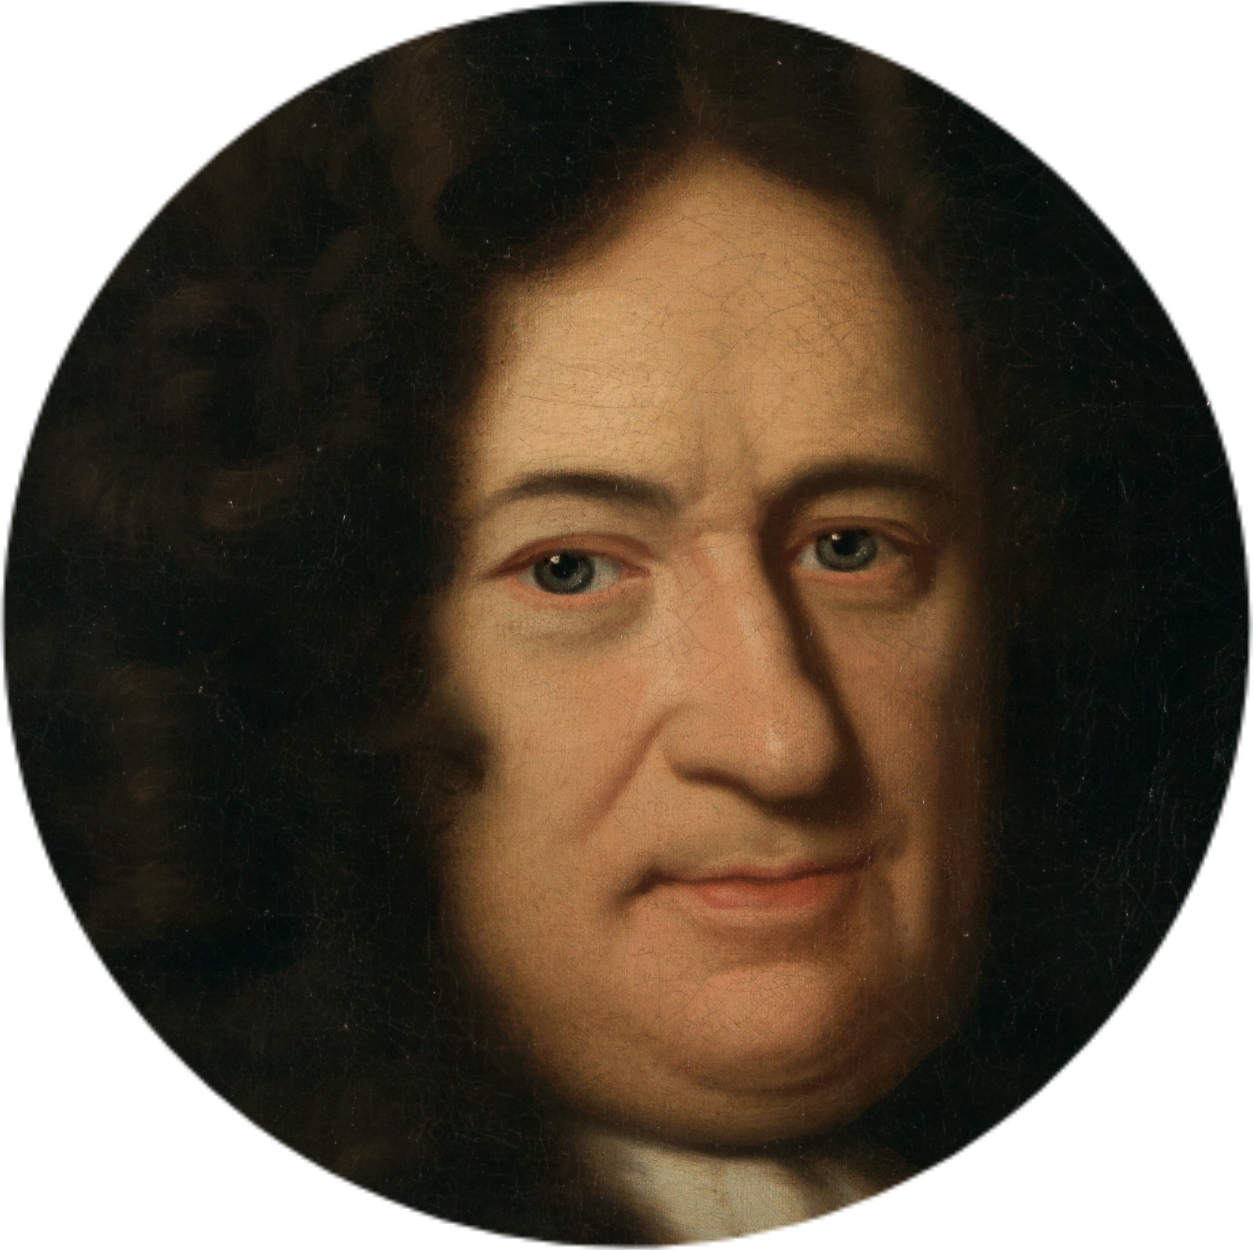
\includegraphics[width=50pt,height=50pt]{Chars/Leibniz.png}};
%Rounded Rect [id:dp5191686460798097] 
\draw  [color={rgb, 255:red, 0; green, 92; blue, 75 }  ,draw opacity=1 ][fill={rgb, 255:red, 0; green, 92; blue, 75 }  ,fill opacity=1 ] (220,156) .. controls (220,147.16) and (227.16,140) .. (236,140) -- (594,140) .. controls (602.84,140) and (610,147.16) .. (610,156) -- (610,204) .. controls (610,212.84) and (602.84,220) .. (594,220) -- (236,220) .. controls (227.16,220) and (220,212.84) .. (220,204) -- cycle ;
%Shape: Half Frame [id:dp24376031746043192] 
\draw  [color={rgb, 255:red, 0; green, 92; blue, 75 }  ,draw opacity=1 ][fill={rgb, 255:red, 0; green, 92; blue, 75 }  ,fill opacity=1 ] (550,140) -- (620,140) -- (599.33,161) -- (571,161) -- (571,189.78) -- (550,211.11) -- cycle ;
%Rounded Rect [id:dp8643336147561154] 
\draw  [color={rgb, 255:red, 54; green, 54; blue, 54 }  ,draw opacity=1 ][fill={rgb, 255:red, 54; green, 54; blue, 54 }  ,fill opacity=1 ] (310,254) .. controls (310,246.27) and (303.73,240) .. (296,240) -- (94,240) .. controls (86.27,240) and (80,246.27) .. (80,254) -- (80,296) .. controls (80,303.73) and (86.27,310) .. (94,310) -- (296,310) .. controls (303.73,310) and (310,303.73) .. (310,296) -- cycle ;
%Shape: Half Frame [id:dp877260980086666] 
\draw  [color={rgb, 255:red, 54; green, 54; blue, 54 }  ,draw opacity=1 ][fill={rgb, 255:red, 54; green, 54; blue, 54 }  ,fill opacity=1 ] (140,240) -- (70,240) -- (91,261) -- (119,261) -- (119,289) -- (140,310) -- cycle ;
%Rounded Rect [id:dp7164157181224868] 
\draw  [color={rgb, 255:red, 54; green, 54; blue, 54 }  ,draw opacity=1 ][fill={rgb, 255:red, 54; green, 54; blue, 54 }  ,fill opacity=1 ] (330,104) .. controls (330,101.79) and (328.21,100) .. (326,100) -- (294,100) .. controls (291.79,100) and (290,101.79) .. (290,104) -- (290,116) .. controls (290,118.21) and (291.79,120) .. (294,120) -- (326,120) .. controls (328.21,120) and (330,118.21) .. (330,116) -- cycle ;
%Rounded Rect [id:dp8914078756100403] 
\draw  [color={rgb, 255:red, 0; green, 92; blue, 75 }  ,draw opacity=1 ][fill={rgb, 255:red, 0; green, 92; blue, 75 }  ,fill opacity=1 ] (220,366) .. controls (220,357.16) and (227.16,350) .. (236,350) -- (594,350) .. controls (602.84,350) and (610,357.16) .. (610,366) -- (610,414) .. controls (610,422.84) and (602.84,430) .. (594,430) -- (236,430) .. controls (227.16,430) and (220,422.84) .. (220,414) -- cycle ;
%Shape: Half Frame [id:dp019193432268682198] 
\draw  [color={rgb, 255:red, 0; green, 92; blue, 75 }  ,draw opacity=1 ][fill={rgb, 255:red, 0; green, 92; blue, 75 }  ,fill opacity=1 ] (550,350) -- (620,350) -- (599.33,371) -- (571,371) -- (571,399.78) -- (550,421.11) -- cycle ;
%Rounded Rect [id:dp21634374173424842] 
\draw  [color={rgb, 255:red, 54; green, 54; blue, 54 }  ,draw opacity=1 ][fill={rgb, 255:red, 54; green, 54; blue, 54 }  ,fill opacity=1 ] (380,324) .. controls (380,321.79) and (378.21,320) .. (376,320) -- (234,320) .. controls (231.79,320) and (230,321.79) .. (230,324) -- (230,336) .. controls (230,338.21) and (231.79,340) .. (234,340) -- (376,340) .. controls (378.21,340) and (380,338.21) .. (380,336) -- cycle ;
%Image [id:dp8518693946864191] 
\draw (35,241.95) node  {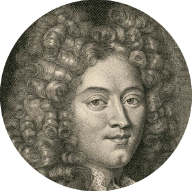
\includegraphics[width=50pt,height=50pt]{Chars/lHopital.png}};
%Image [id:dp7198452370903958] 
\draw (655,351.83) node  {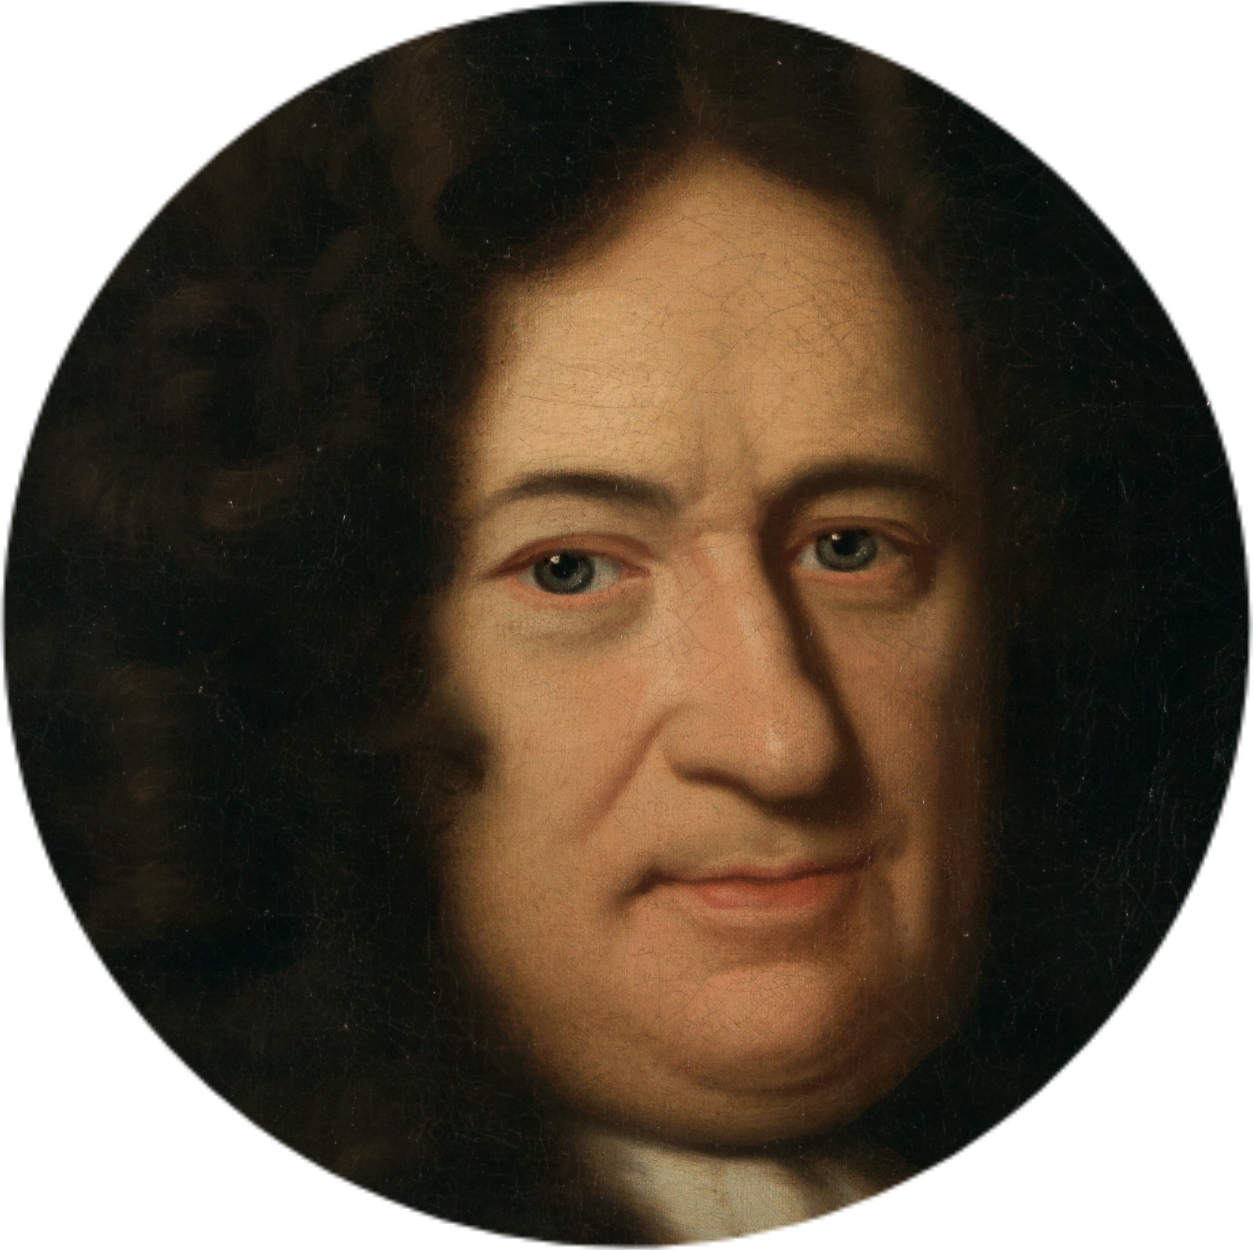
\includegraphics[width=50pt,height=50pt]{Chars/Leibniz.png}};
% Text Node
\draw (231,162.17) node [anchor=north west][inner sep=0.75pt]  [font=\large,color={rgb, 255:red, 252; green, 252; blue, 252 }  ,opacity=1 ] [align=left] {Can the meaning of derivative with integer order be \\generalized to derivative with non-integer order?!};
% Text Node
\draw (91,257.75) node [anchor=north west][inner sep=0.75pt]  [font=\large,color={rgb, 255:red, 252; green, 252; blue, 252 }  ,opacity=1 ] [align=left] {What if the order will be $\displaystyle \frac{1}{2}$?!};

% Text Node
\draw (552,143) node [anchor=north west][inner sep=0.75pt]  [color={rgb, 255:red, 255; green, 215; blue, 0 }  ,opacity=1 ] [align=left] {Leibniz};
% Text Node
\draw (94,244.83) node [anchor=north west][inner sep=0.75pt]  [color={rgb, 255:red, 255; green, 215; blue, 0 }  ,opacity=1 ] [align=left] {L'Hopital};
% Text Node
\draw (581,202) node [anchor=north west][inner sep=0.75pt]  [color={rgb, 255:red, 57; green, 159; blue, 185 }  ,opacity=1 ] [align=left] {$\surd$};
% Text Node
\draw (584,202) node [anchor=north west][inner sep=0.75pt]  [color={rgb, 255:red, 57; green, 159; blue, 185 }  ,opacity=1 ] [align=left] {$\surd$};
% Text Node
\draw (291,102) node [anchor=north west][inner sep=0.75pt]  [font=\large , color={rgb, 255:red, 254; green, 254; blue, 254 }  ,opacity=1 ] [align=left] {1695};
% Text Node
\draw (91,292) node [anchor=north west][inner sep=0.75pt]  [color={rgb, 255:red, 57; green, 159; blue, 185 }  ,opacity=1 ] [align=left] {$\surd$};
% Text Node
\draw (94,292) node [anchor=north west][inner sep=0.75pt]  [color={rgb, 255:red, 57; green, 159; blue, 185 }  ,opacity=1 ] [align=left] {$\surd$};
% Text Node
\draw (231,372.17) node [anchor=north west][inner sep=0.75pt]  [font=\large , color={rgb, 255:red, 252; green, 252; blue, 252 }  ,opacity=1 ] [align=left] {It will lead to a paradox, from which one day useful \\consequences will be drawn};
% Text Node
\draw (581,412) node [anchor=north west][inner sep=0.75pt]  [color={rgb, 255:red, 57; green, 159; blue, 185 }  ,opacity=1 ] [align=left] {$\surd$};
% Text Node
\draw (584,412) node [anchor=north west][inner sep=0.75pt]  [color={rgb, 255:red, 57; green, 159; blue, 185 }  ,opacity=1 ] [align=left] {$\surd$};
% Text Node
\draw (236,323) node [anchor=north west][inner sep=0.75pt]  [font=\large , color={rgb, 255:red, 254; green, 254; blue, 254 }  ,opacity=1 ] [align=left] {September 30, 1695};
% Text Node
\draw (551,352) node [anchor=north west][inner sep=0.75pt]  [color={rgb, 255:red, 255; green, 215; blue, 0 }  ,opacity=1 ] [align=left] {Leibniz};
\end{tikzpicture}
\end{figure*}
\endgroup











                 % The pages in the End
%%%%%%%%%%%%%%%%%%%%%%%%%%%%%%%%%%%%%%%%%%%%%%%%%%%%%%%%%%%%
%%%%%%%%%%%%%%%%%%%%%%%%%%%%%%%%%%%%%%%%%%%%%%%%%%%%%%%%%%%%
%%%%%%%%%%%%%%%%%%%%%%%%%%%%%%%%%%%%%%%%%%%%%%%%%%%%%%%%%%%%
%%%%%%%%%%%%%%%%%%%%%%%%%%%%%%%%%%%%%%%%%%%%%%%%%%%%%%%%%%%%
%%%%%%%%%%%%%%%%%%%%%%%%%%%%%%%%%%%%%%%%%%%%%%%%%%%%%%%%%%%%
%%%%%%%%%%%%%%%%%%%%%%%%%%%%%%%%%%%%%%%%%%%%%%%%%%%%%%%%%%%%
%%%%%%%%%%%%%%%%%%%%%%%%%%%%%%%%%%%%%%%%%%%%%%%%%%%%%%%%%%%%


% \newpage


\hspace*{1.5cm}
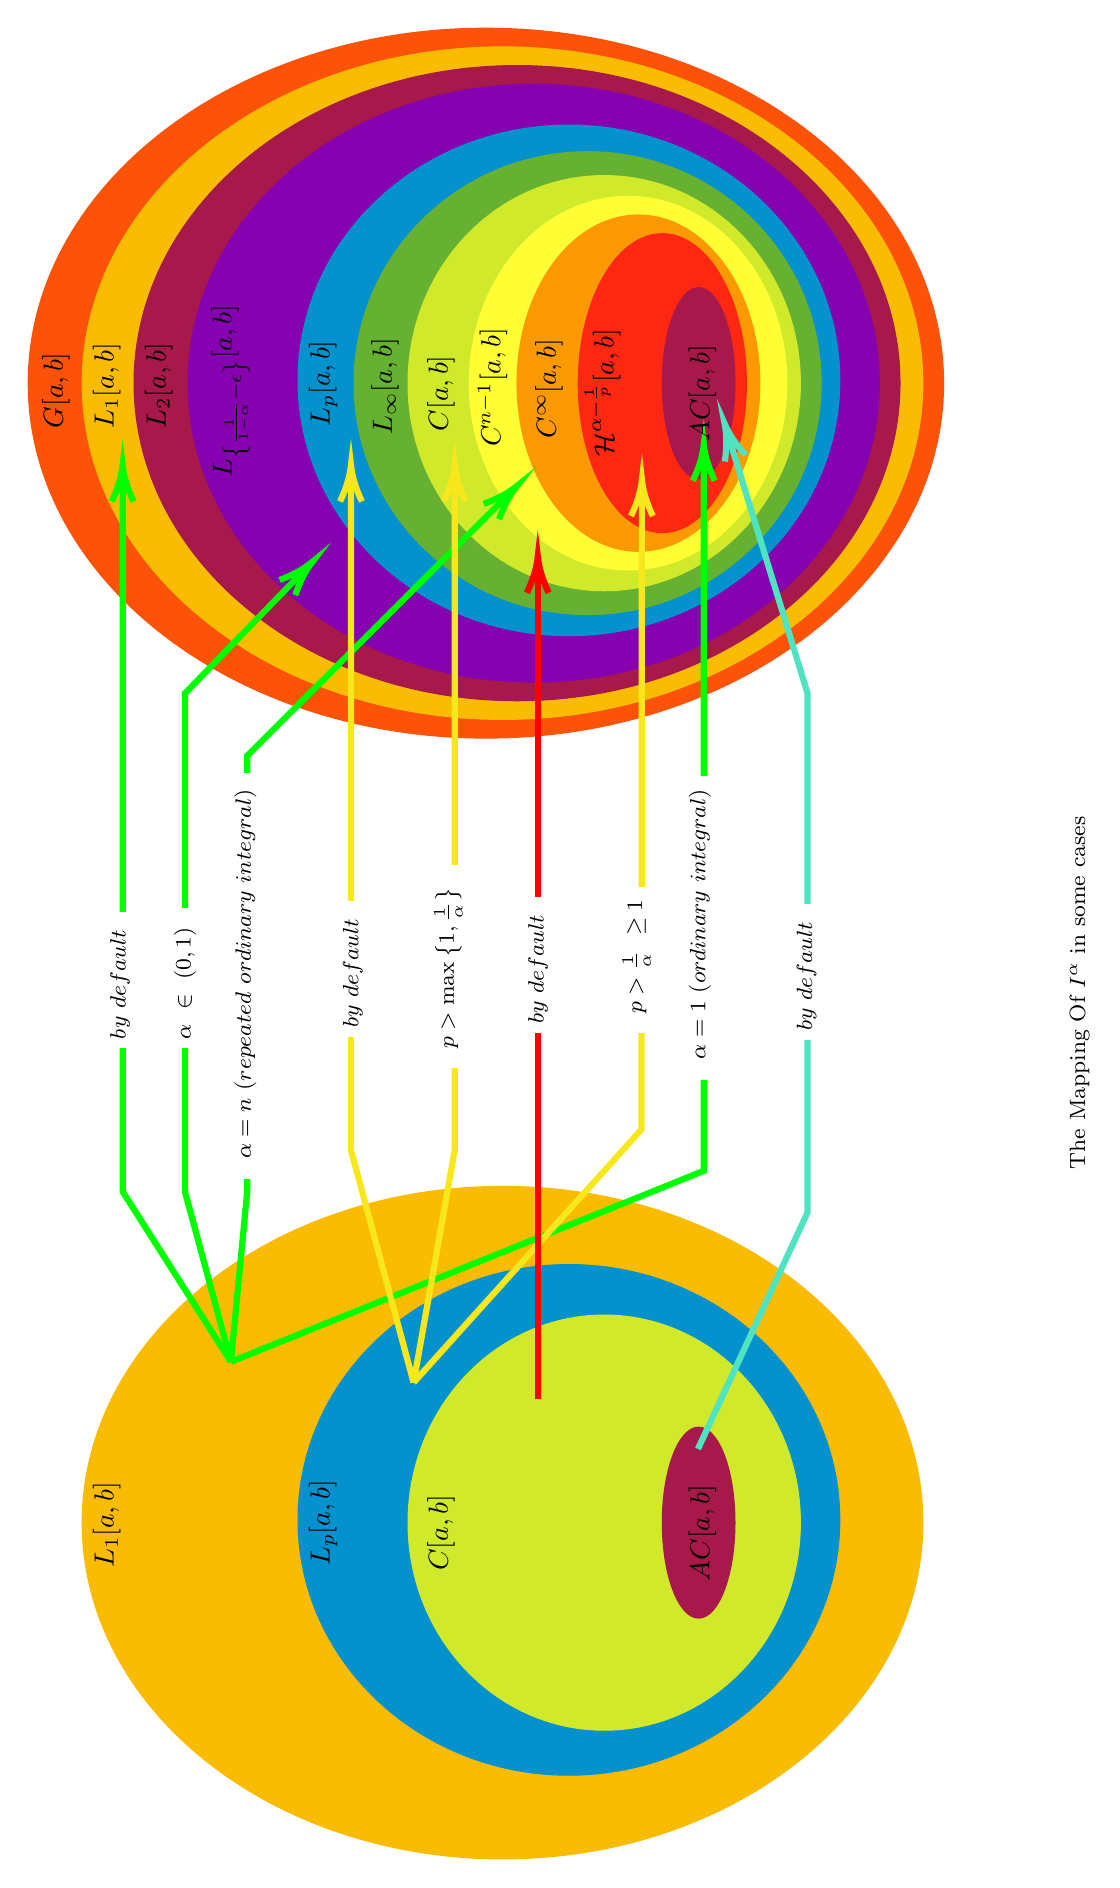
\begin{tikzpicture}[x=0.75pt,y=0.75pt,yscale=-1,xscale=1,scale=1]
%uncomment if require: \path (0,1171); %set diagram left start at 0, and has height of 1171

%Shape: Ellipse [id:dp36421966981860576] 
\draw  [color={rgb, 255:red, 253; green, 83; blue, 8 }  ,draw opacity=1 ][fill={rgb, 255:red, 253; green, 83; blue, 8 }  ,fill opacity=1 ] (320.5,376) .. controls (198.72,376) and (100,299.44) .. (100,205) .. controls (100,110.56) and (198.72,34) .. (320.5,34) .. controls (442.28,34) and (541,110.56) .. (541,205) .. controls (541,299.44) and (442.28,376) .. (320.5,376) -- cycle ;
%Shape: Ellipse [id:dp513596341046219] 
\draw  [color={rgb, 255:red, 249; green, 188; blue, 2 }  ,draw opacity=1 ][fill={rgb, 255:red, 249; green, 188; blue, 2 }  ,fill opacity=1 ] (328.5,367) .. controls (216.66,367) and (126,294.47) .. (126,205) .. controls (126,115.53) and (216.66,43) .. (328.5,43) .. controls (440.34,43) and (531,115.53) .. (531,205) .. controls (531,294.47) and (440.34,367) .. (328.5,367) -- cycle ;
%Shape: Ellipse [id:dp8342256600903095] 
\draw  [color={rgb, 255:red, 167; green, 25; blue, 75 }  ,draw opacity=1 ][fill={rgb, 255:red, 167; green, 25; blue, 75 }  ,fill opacity=1 ] (335.5,358) .. controls (233.6,358) and (151,289.5) .. (151,205) .. controls (151,120.5) and (233.6,52) .. (335.5,52) .. controls (437.4,52) and (520,120.5) .. (520,205) .. controls (520,289.5) and (437.4,358) .. (335.5,358) -- cycle ;
%Shape: Ellipse [id:dp7701966259035993] 
\draw  [color={rgb, 255:red, 134; green, 1; blue, 176 }  ,draw opacity=1 ][fill={rgb, 255:red, 134; green, 1; blue, 176 }  ,fill opacity=1 ] (343.5,349) .. controls (251.54,349) and (177,284.53) .. (177,205) .. controls (177,125.47) and (251.54,61) .. (343.5,61) .. controls (435.46,61) and (510,125.47) .. (510,205) .. controls (510,284.53) and (435.46,349) .. (343.5,349) -- cycle ;
%Shape: Ellipse [id:dp8718526137926743] 
\draw  [color={rgb, 255:red, 3; green, 146; blue, 206 }  ,draw opacity=1 ][fill={rgb, 255:red, 3; green, 146; blue, 206 }  ,fill opacity=1 ] (360.5,326.67) .. controls (288.43,326.67) and (230,271.6) .. (230,203.67) .. controls (230,135.74) and (288.43,80.67) .. (360.5,80.67) .. controls (432.57,80.67) and (491,135.74) .. (491,203.67) .. controls (491,271.6) and (432.57,326.67) .. (360.5,326.67) -- cycle ;
%Shape: Ellipse [id:dp07229888839358667] 
\draw  [color={rgb, 255:red, 102; green, 177; blue, 50 }  ,draw opacity=1 ][fill={rgb, 255:red, 102; green, 177; blue, 50 }  ,fill opacity=1 ] (369.5,316.5) .. controls (307.37,316.5) and (257,266.58) .. (257,205) .. controls (257,143.42) and (307.37,93.5) .. (369.5,93.5) .. controls (431.63,93.5) and (482,143.42) .. (482,205) .. controls (482,266.58) and (431.63,316.5) .. (369.5,316.5) -- cycle ;
%Shape: Ellipse [id:dp26102978707270297] 
\draw  [color={rgb, 255:red, 208; green, 233; blue, 43 }  ,draw opacity=1 ][fill={rgb, 255:red, 208; green, 233; blue, 43 }  ,fill opacity=1 ] (377.5,305) .. controls (325.31,305) and (283,260.23) .. (283,205) .. controls (283,149.77) and (325.31,105) .. (377.5,105) .. controls (429.69,105) and (472,149.77) .. (472,205) .. controls (472,260.23) and (429.69,305) .. (377.5,305) -- cycle ;
%Shape: Ellipse [id:dp3143329621107056] 
\draw  [color={rgb, 255:red, 255; green, 254; blue, 52 }  ,draw opacity=1 ][fill={rgb, 255:red, 255; green, 254; blue, 52 }  ,fill opacity=1 ] (389,295) .. controls (346.75,295) and (312.5,254.71) .. (312.5,205) .. controls (312.5,155.29) and (346.75,115) .. (389,115) .. controls (431.25,115) and (465.5,155.29) .. (465.5,205) .. controls (465.5,254.71) and (431.25,295) .. (389,295) -- cycle ;
%Shape: Ellipse [id:dp49451773436571855] 
\draw  [color={rgb, 255:red, 251; green, 153; blue, 2 }  ,draw opacity=1 ][fill={rgb, 255:red, 251; green, 153; blue, 2 }  ,fill opacity=1 ] (394,286) .. controls (361.69,286) and (335.5,249.74) .. (335.5,205) .. controls (335.5,160.26) and (361.69,124) .. (394,124) .. controls (426.31,124) and (452.5,160.26) .. (452.5,205) .. controls (452.5,249.74) and (426.31,286) .. (394,286) -- cycle ;
%Shape: Ellipse [id:dp7286874747001277] 
\draw  [color={rgb, 255:red, 254; green, 39; blue, 18 }  ,draw opacity=1 ][fill={rgb, 255:red, 254; green, 39; blue, 18 }  ,fill opacity=1 ] (405.5,277) .. controls (383.13,277) and (365,244.76) .. (365,205) .. controls (365,165.24) and (383.13,133) .. (405.5,133) .. controls (427.87,133) and (446,165.24) .. (446,205) .. controls (446,244.76) and (427.87,277) .. (405.5,277) -- cycle ;
%Shape: Ellipse [id:dp9160012222939253] 
\draw  [color={rgb, 255:red, 167; green, 25; blue, 75 }  ,draw opacity=1 ][fill={rgb, 255:red, 167; green, 25; blue, 75 }  ,fill opacity=1 ] (423,251) .. controls (413.34,251) and (405.5,230.41) .. (405.5,205) .. controls (405.5,179.59) and (413.34,159) .. (423,159) .. controls (432.66,159) and (440.5,179.59) .. (440.5,205) .. controls (440.5,230.41) and (432.66,251) .. (423,251) -- cycle ;

%Shape: Ellipse [id:dp7687741619822284] 
\draw  [color={rgb, 255:red, 249; green, 188; blue, 2 }  ,draw opacity=1 ][fill={rgb, 255:red, 249; green, 188; blue, 2 }  ,fill opacity=1 ] (328.5,916) .. controls (216.66,916) and (126,843.47) .. (126,754) .. controls (126,664.53) and (216.66,592) .. (328.5,592) .. controls (440.34,592) and (531,664.53) .. (531,754) .. controls (531,843.47) and (440.34,916) .. (328.5,916) -- cycle ;
%Shape: Ellipse [id:dp7863689832047069] 
\draw  [color={rgb, 255:red, 3; green, 146; blue, 206 }  ,draw opacity=1 ][fill={rgb, 255:red, 3; green, 146; blue, 206 }  ,fill opacity=1 ] (360.5,875.67) .. controls (288.43,875.67) and (230,820.6) .. (230,752.67) .. controls (230,684.74) and (288.43,629.67) .. (360.5,629.67) .. controls (432.57,629.67) and (491,684.74) .. (491,752.67) .. controls (491,820.6) and (432.57,875.67) .. (360.5,875.67) -- cycle ;
%Shape: Ellipse [id:dp36197594607695427] 
\draw  [color={rgb, 255:red, 208; green, 233; blue, 43 }  ,draw opacity=1 ][fill={rgb, 255:red, 208; green, 233; blue, 43 }  ,fill opacity=1 ] (377.5,854) .. controls (325.31,854) and (283,809.23) .. (283,754) .. controls (283,698.77) and (325.31,654) .. (377.5,654) .. controls (429.69,654) and (472,698.77) .. (472,754) .. controls (472,809.23) and (429.69,854) .. (377.5,854) -- cycle ;
%Shape: Ellipse [id:dp8626838071461165] 
\draw  [color={rgb, 255:red, 167; green, 25; blue, 75 }  ,draw opacity=1 ][fill={rgb, 255:red, 167; green, 25; blue, 75 }  ,fill opacity=1 ] (423,800) .. controls (413.34,800) and (405.5,779.41) .. (405.5,754) .. controls (405.5,728.59) and (413.34,708) .. (423,708) .. controls (432.66,708) and (440.5,728.59) .. (440.5,754) .. controls (440.5,779.41) and (432.66,800) .. (423,800) -- cycle ;


%Straight Lines [id:da29740484436841275] 
\draw [color={rgb, 255:red, 0; green, 255; blue, 0 }  ,draw opacity=1 ][line width=2.25]    (197.67,676.5) -- (145.5,594.5) -- (145.5,248.5) ;
\draw [shift={(145.5,244.5)}, rotate = 90] [color={rgb, 255:red, 0; green, 255; blue, 0 }  ,draw opacity=1 ][line width=2.25]    (17.49,-5.26) .. controls (11.12,-2.23) and (5.29,-0.48) .. (0,0) .. controls (5.29,0.48) and (11.12,2.23) .. (17.49,5.26)   ;
%Straight Lines [id:da747322555087151] 
\draw [color={rgb, 255:red, 0; green, 255; blue, 0 }  ,draw opacity=1 ][line width=2.25]    (197.67,676.5) -- (425.5,584.5) -- (425.5,238.5) ;
\draw [shift={(425.5,234.5)}, rotate = 90] [color={rgb, 255:red, 0; green, 255; blue, 0 }  ,draw opacity=1 ][line width=2.25]    (17.49,-5.26) .. controls (11.12,-2.23) and (5.29,-0.48) .. (0,0) .. controls (5.29,0.48) and (11.12,2.23) .. (17.49,5.26)   ;
%Straight Lines [id:da3355128348747227] 
\draw [color={rgb, 255:red, 0; green, 255; blue, 0 }  ,draw opacity=1 ][line width=2.25]    (197.67,676.5) -- (205.5,594.5) -- (205.5,384.5) -- (332.67,257.33) ;
\draw [shift={(335.5,254.5)}, rotate = 135] [color={rgb, 255:red, 0; green, 255; blue, 0 }  ,draw opacity=1 ][line width=2.25]    (17.49,-5.26) .. controls (11.12,-2.23) and (5.29,-0.48) .. (0,0) .. controls (5.29,0.48) and (11.12,2.23) .. (17.49,5.26)   ;
%Straight Lines [id:da5987549368234755] 
\draw [color={rgb, 255:red, 0; green, 255; blue, 0 }  ,draw opacity=1 ][line width=2.25]    (197.67,676.5) -- (175.5,594.5) -- (175.5,354.5) -- (234.27,293.82) ;
\draw [shift={(237.06,290.94)}, rotate = 134.08] [color={rgb, 255:red, 0; green, 255; blue, 0 }  ,draw opacity=1 ][line width=2.25]    (17.49,-5.26) .. controls (11.12,-2.23) and (5.29,-0.48) .. (0,0) .. controls (5.29,0.48) and (11.12,2.23) .. (17.49,5.26)   ;

%Straight Lines [id:da3971858139126001] 
\draw [color={rgb, 255:red, 248; green, 231; blue, 28 }  ,draw opacity=1 ][line width=2.25]    (285.67,686.5) -- (255.5,574.5) -- (255.5,248.5) ;
\draw [shift={(255.5,244.5)}, rotate = 90] [color={rgb, 255:red, 248; green, 231; blue, 28 }  ,draw opacity=1 ][line width=2.25]    (17.49,-5.26) .. controls (11.12,-2.23) and (5.29,-0.48) .. (0,0) .. controls (5.29,0.48) and (11.12,2.23) .. (17.49,5.26)   ;
%Straight Lines [id:da680452400138468] 
\draw [color={rgb, 255:red, 248; green, 231; blue, 28 }  ,draw opacity=1 ][line width=2.25]    (285.67,686.5) -- (305.5,574.5) -- (305.5,248.5) ;
\draw [shift={(305.5,244.5)}, rotate = 90] [color={rgb, 255:red, 248; green, 231; blue, 28 }  ,draw opacity=1 ][line width=2.25]    (17.49,-5.26) .. controls (11.12,-2.23) and (5.29,-0.48) .. (0,0) .. controls (5.29,0.48) and (11.12,2.23) .. (17.49,5.26)   ;
%Straight Lines [id:da03005347223035426] 
\draw [color={rgb, 255:red, 248; green, 231; blue, 28 }  ,draw opacity=1 ][line width=2.25]    (285.67,686.5) -- (395.5,564.5) -- (395.66,255.5) ;
\draw [shift={(395.67,251.5)}, rotate = 90.03] [color={rgb, 255:red, 248; green, 231; blue, 28 }  ,draw opacity=1 ][line width=2.25]    (17.49,-5.26) .. controls (11.12,-2.23) and (5.29,-0.48) .. (0,0) .. controls (5.29,0.48) and (11.12,2.23) .. (17.49,5.26)   ;

%Straight Lines [id:da15460774860319515] 
\draw [color={rgb, 255:red, 255; green, 0; blue, 0 }  ,draw opacity=1 ][line width=2.25]    (345.5,694.5) -- (345.5,292.5) ;
\draw [shift={(345.5,288.5)}, rotate = 90] [color={rgb, 255:red, 255; green, 0; blue, 0 }  ,draw opacity=1 ][line width=2.25]    (17.49,-5.26) .. controls (11.12,-2.23) and (5.29,-0.48) .. (0,0) .. controls (5.29,0.48) and (11.12,2.23) .. (17.49,5.26)   ;
%Straight Lines [id:da43732852110852893] 
\draw [color={rgb, 255:red, 80; green, 227; blue, 194 }  ,draw opacity=1 ][line width=2.25]    (422.67,718.5) -- (475.5,604.5) -- (475.5,354.5) -- (436.68,228.32) ;
\draw [shift={(435.5,224.5)}, rotate = 72.9] [color={rgb, 255:red, 80; green, 227; blue, 194 }  ,draw opacity=1 ][line width=2.25]    (17.49,-5.26) .. controls (11.12,-2.23) and (5.29,-0.48) .. (0,0) .. controls (5.29,0.48) and (11.12,2.23) .. (17.49,5.26)   ;


% Text Node
\draw (105.4,228) node [anchor=north west][inner sep=0.75pt]  [rotate=-270]  {$G[ a,b]$};
% Text Node
\draw (129.9,228) node [anchor=north west][inner sep=0.75pt]  [rotate=-270]  {$L_{1}[ a,b]$};
% Text Node
\draw (154.9,228) node [anchor=north west][inner sep=0.75pt]  [rotate=-270]  {$L_{2}[ a,b]$};
% Text Node
\draw (263.9,231) node [anchor=north west][inner sep=0.75pt]  [rotate=-270]  {$L_{\infty }[ a,b]$};
% Text Node
\draw (233.9,227) node [anchor=north west][inner sep=0.75pt]  [rotate=-270]  {$L_{p}[ a,b]$};
% Text Node
\draw (290.9,229.5) node [anchor=north west][inner sep=0.75pt]  [rotate=-270]  {$C[ a,b]$};
% Text Node
\draw (366.9,241.5) node [anchor=north west][inner sep=0.75pt]  [rotate=-270]  {$\mathcal{H}^{\alpha -\frac{1}{p}}[ a,b]$};
% Text Node
\draw (416.9,234.5) node [anchor=north west][inner sep=0.75pt]  [rotate=-270]  {$AC[ a,b]$};
% Text Node
\draw (342.9,233) node [anchor=north west][inner sep=0.75pt]  [rotate=-270]  {$C^{\infty }[ a,b]$};
% Text Node
\draw (315.4,237) node [anchor=north west][inner sep=0.75pt]  [rotate=-270]  {$C^{n-1}[ a,b]$};
% Text Node
\draw (186.9,251.5) node [anchor=north west][inner sep=0.75pt]  [rotate=-270]  {$L_{\left\{\frac{1}{1-\alpha } -\epsilon \right\}}[ a,b]$};
% Text Node
\draw (129.9,777) node [anchor=north west][inner sep=0.75pt]  [rotate=-270]  {$L_{1}[ a,b]$};
% Text Node
\draw (233.9,776) node [anchor=north west][inner sep=0.75pt]  [rotate=-270]  {$L_{p}[ a,b]$};
% Text Node
\draw (290.9,778.5) node [anchor=north west][inner sep=0.75pt]  [rotate=-270]  {$C[ a,b]$};
% Text Node
\draw (416.9,783.5) node [anchor=north west][inner sep=0.75pt]  [rotate=-270]  {$AC[ a,b]$};
% Text Node
\draw  [color={rgb, 255:red, 255; green, 255; blue, 255 }  ,draw opacity=1 ][fill={rgb, 255:red, 255; green, 255; blue, 255 }  ,fill opacity=1 ]  (279.94,437.61) -- (327.94,437.61) -- (327.94,534.61) -- (279.94,534.61) -- cycle  ;
\draw (294.34,527) node [anchor=north west][inner sep=0.75pt]  [font=\footnotesize,rotate=-270]  {$p >\max\left\{1,\frac{1}{\alpha }\right\}$};
% Text Node
\draw  [color={rgb, 255:red, 255; green, 255; blue, 255 }  ,draw opacity=1 ][fill={rgb, 255:red, 255; green, 255; blue, 255 }  ,fill opacity=1 ]  (335.28,452.94) -- (355.28,452.94) -- (355.28,517.94) -- (335.28,517.94) -- cycle  ;
\draw (339.68,514.94) node [anchor=north west][inner sep=0.75pt]  [font=\footnotesize,rotate=-270]  {$by\ default$};
% Text Node
\draw  [color={rgb, 255:red, 255; green, 255; blue, 255 }  ,draw opacity=1 ][fill={rgb, 255:red, 255; green, 255; blue, 255 }  ,fill opacity=1 ]  (464.61,456.28) -- (484.61,456.28) -- (484.61,521.28) -- (464.61,521.28) -- cycle  ;
\draw (469.01,518.28) node [anchor=north west][inner sep=0.75pt]  [font=\footnotesize,rotate=-270]  {$by\ default$};
% Text Node
\draw  [color={rgb, 255:red, 255; green, 255; blue, 255 }  ,draw opacity=1 ][fill={rgb, 255:red, 255; green, 255; blue, 255 }  ,fill opacity=1 ]  (245.94,454.94) -- (265.94,454.94) -- (265.94,519.94) -- (245.94,519.94) -- cycle  ;
\draw (250.34,516.94) node [anchor=north west][inner sep=0.75pt]  [font=\footnotesize,rotate=-270]  {$by\ default$};
% Text Node
\draw  [color={rgb, 255:red, 255; green, 255; blue, 255 }  ,draw opacity=1 ][fill={rgb, 255:red, 255; green, 255; blue, 255 }  ,fill opacity=1 ]  (133.85,460.28) -- (153.85,460.28) -- (153.85,525.28) -- (133.85,525.28) -- cycle  ;
\draw (138.25,522.28) node [anchor=north west][inner sep=0.75pt]  [font=\footnotesize,rotate=-270]  {$by\ default$};
% Text Node
\draw  [color={rgb, 255:red, 255; green, 255; blue, 255 }  ,draw opacity=1 ][fill={rgb, 255:red, 255; green, 255; blue, 255 }  ,fill opacity=1 ]  (164.52,458.28) -- (184.52,458.28) -- (184.52,525.28) -- (164.52,525.28) -- cycle  ;
\draw (168.92,522.28) node [anchor=north west][inner sep=0.75pt]  [font=\footnotesize,rotate=-270]  {$\alpha \ \in \ ( 0,1)$};
% Text Node
\draw  [color={rgb, 255:red, 255; green, 255; blue, 255 }  ,draw opacity=1 ][fill={rgb, 255:red, 255; green, 255; blue, 255 }  ,fill opacity=1 ]  (374.17,447.94) -- (411.17,447.94) -- (411.17,517.94) -- (374.17,517.94) -- cycle  ;
\draw (385,510) node [anchor=north west][inner sep=0.75pt]  [font=\footnotesize,rotate=-270]  {$p >\frac{1}{\alpha } \ \geq 1$};
% Text Node
\draw  [color={rgb, 255:red, 255; green, 255; blue, 255 }  ,draw opacity=1 ][fill={rgb, 255:red, 255; green, 255; blue, 255 }  ,fill opacity=1 ]  (415.28,394.61) -- (435.28,394.61) -- (435.28,540.61) -- (415.28,540.61) -- cycle  ;
\draw (417,532) node [anchor=north west][inner sep=0.75pt]  [font=\footnotesize,rotate=-270]  {$\alpha =1\ ( ordinary\ integral)$};
% Text Node
\draw  [color={rgb, 255:red, 255; green, 255; blue, 255 }  ,draw opacity=1 ][fill={rgb, 255:red, 255; green, 255; blue, 255 }  ,fill opacity=1 ]  (196.08,392.94) -- (216.08,392.94) -- (216.08,587.94) -- (196.08,587.94) -- cycle  ;
\draw (198,580) node [anchor=north west][inner sep=0.75pt]  [font=\footnotesize,rotate=-270]  {$\alpha =n\ ( repeated\ ordinary\ integral)$};
\draw (600.48,584.94) node [anchor=north west][inner sep=0.75pt]  [font=\footnotesize,rotate=-270]  {The Mapping Of $I^{\alpha}$ in some cases};

\end{tikzpicture}


\newpage


                % (working on) Part   














% \begin{equation*}
%         \label{eq:aaa} \tag{$\star$} \forall \epsilon
% \end{equation*}
% \begin{equation*}
%         \label{eq:aab} \tag{5.25} \exists \delta
% \end{equation*}
% this is ref to equation (\ref{eq:aab})
% \begin{example}
%         \label{ex:aaa} solve 
% \end{example}
% this is ref to example (\ref{ex:aaa})
% \begin{theorem}[convergent]
%         \label{thm:aaa} 
%         from (\ref{eq:aaa}) and (\ref{eq:aab}) then it's done
% \end{theorem}
% this is ref to theorem (\ref{thm:aaa})

% \begin{center}
%         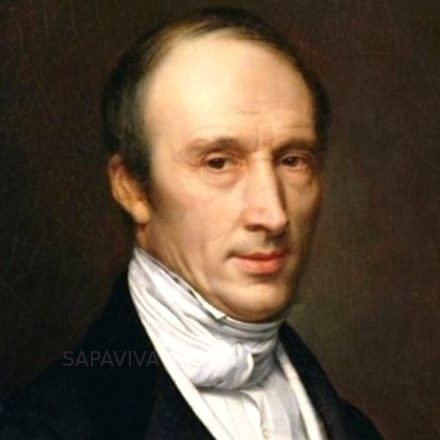
\includegraphics[width = 5cm]{Chars/Cauchy.jpg}
% \end{center}

\end{document}